Hệ thống được đặt tên \textbf{BKareer}.
BKareer được thiết kế và xây dựng dựa trên các công nghệ chính sau:
\begin{itemize}
    \item \textbf{Hệ cơ sở dữ liệu MongoDB Atlas:} Hệ thống sử dụng MongoDB Atlas làm cơ sở dữ liệu để lưu trữ và quản lý các thông tin về ngành nghề, các trường đại học, và dữ liệu người dùng khác. MongoDB Atlas được chọn vì tính linh hoạt, khả năng mở rộng và sự dễ dàng trong quản lý.
    \item \textbf{Hệ thống API và thuật toán trên framework Flask của Python:} Việc xây dựng các API và xử lý thuật toán được thực hiện trên framework Flask của Python. Flask cung cấp một cách tiếp cận linh hoạt và dễ dàng để phát triển các ứng dụng web, đồng thời hỗ trợ việc xây dựng các RESTful API để tương tác với dữ liệu từ hệ cơ sở dữ liệu.
    \item \textbf{Hệ thống xử lý yêu cầu người dùng} Được xây dựng trên Nodejs-Express. Cung cấp api và các tính năng liên quan tới người dùng cuối thông qua việc tương tác với server nhằm lưu trữ và truy vấn thông tin. 
    \item \textbf{Giao diện người dùng sử dụng ReactJS:} Giao diện người dùng của hệ thống được phát triển bằng ReactJS, một thư viện JavaScript phổ biến cho việc xây dựng các ứng dụng web.
\end{itemize}

Hệ thống được tổ chức theo cơ chế client-server sử dụng restful API để tương tác giữa các thành phần. Hệ thống được chia thành các thành phần chính sau:
\begin{figure}[H]
    \centering
    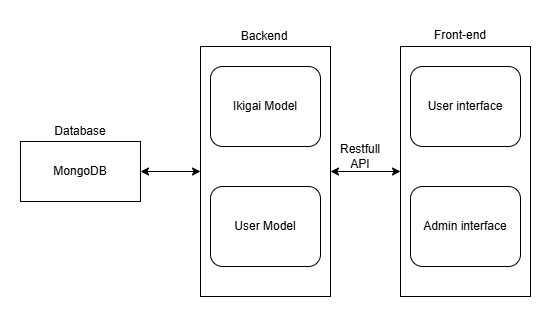
\includegraphics[width=0.7\linewidth]{images/sys.png}
    \vspace{0.5cm}
    \caption{Hệ thống}
\end{figure}

Sau khi hoàn thành và kiểm tra, nhóm đã triển khai hệ thống lên các nền tảng VPS và thuê Domain-name server để hướng tới người dùng cuối. Thông qua giao thức HTTP, các thành phần của giao diện người dùng được yêu cầu và truyền tải từ server đến trình duyệt của người dùng. Điều này đảm bảo rằng người dùng có thể truy cập và tương tác với hệ thống một cách nhanh chóng và ổn định. Cơ sở hạ tầng server được thiết kế để đáp ứng lưu lượng truy cập và đảm bảo tính khả dụng cao.

Server xử lý được triển khai trên nền tảng VPS - virtual private server với IP là 103.15.51.131.
Người dùng có thể truy cập hệ thống qua đường dẫn: \href{http://bkareer.online/}{\color{black}https://bkareer.online/}

%%%%%%%%%%%%%%%%%%%%%%%%%%%% Deploy %%%%%%%%%%%%%%%%%%%%%%%%%%%%
\section{Triển khai hệ thống}

\subsection{Môi trường triển khai}

\subsubsection{VPS}
VPS, hay máy chủ riêng ảo, là một hình thức lưu trữ đám mây đa người thuê, trong đó các tài nguyên máy chủ được ảo hóa và cung cấp cho người dùng qua internet thông qua nhà cung cấp đám mây hoặc lưu trữ. Mỗi VPS được cài đặt trên một máy vật lý, được vận hành bởi nhà cung cấp, và có khả năng chạy nhiều VPS trên cùng một máy. Mặc dù chia sẻ phần cứng cơ bản, mỗi VPS vẫn có hệ điều hành và tài nguyên riêng như bộ nhớ, tính toán, và không bị ảnh hưởng bởi các VPS khác trên cùng máy.

VPS là giải pháp cân bằng giữa lưu trữ chia sẻ thông thường và máy chủ chuyên dụng đơn người thuê, mang lại hiệu suất cao cùng với tính linh hoạt trong quản lý. Mặc dù đây là mô hình đa người thuê, nó được gọi là "riêng tư" vì mỗi người dùng được phân bổ tài nguyên cụ thể và không bị can thiệp bởi người dùng khác. 

\subsubsection{Đăng ký tên miền và chứng chỉ SSL}
Tên miền đóng vai trò là địa chỉ trực tuyến duy nhất, giúp khách hàng dễ dàng tìm thấy website. Việc sở hữu một tên miền không chỉ tăng uy tín mà còn khẳng định mức độ chuyên nghiệp của doanh nghiệp trên thị trường trực tuyến. Đây là cầu nối giữa doanh nghiệp và khách hàng, mở rộng cơ hội kinh doanh và khẳng định thương hiệu trong môi trường kỹ thuật số.

Chứng chỉ SSL (Secure Sockets Layer) là một công cụ quan trọng trong việc bảo mật website, cho phép mã hóa dữ liệu truyền giữa máy chủ và trình duyệt. Điều này không chỉ bảo vệ thông tin khách hàng mà còn tạo dựng niềm tin, đặc biệt trong các giao dịch trực tuyến.

\subsection{Các bước triển khai hệ thống}

\subsubsection{Bước 1: Đăng ký VPS}
Nhóm đã đăng ký VPS tại \textit{matbao.net}. Sau khi mua VPS, nhà cung cấp cung cấp địa chỉ IP và mật khẩu truy cập. Đây là bước đầu để thiết lập môi trường triển khai trên máy chủ riêng. Dưới đây là hình ảnh về server của nhóm.

\begin{figure}[H]
    \centering
    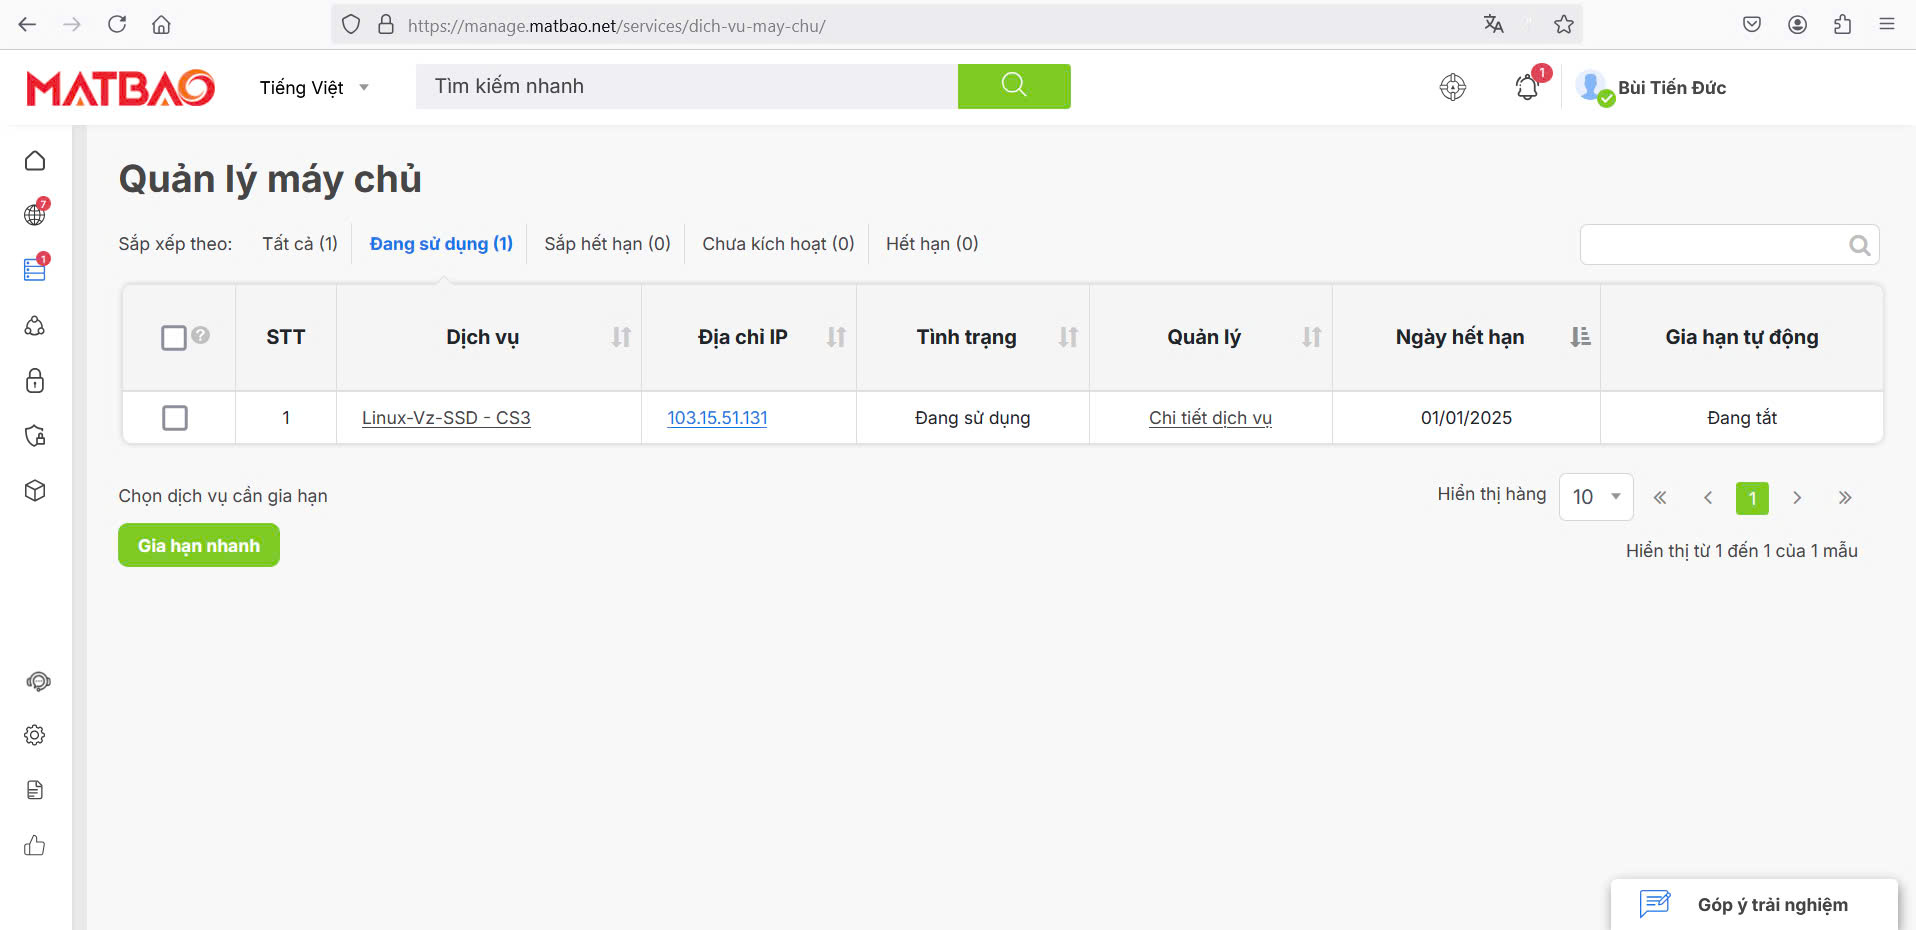
\includegraphics[width=0.8\linewidth]{images/vps1.jpg}
    \vspace{0.5cm}
    \caption{Thông tin VPS}
    % \caption{Hệ thống}
\end{figure}

\begin{figure}[H]
    \centering
    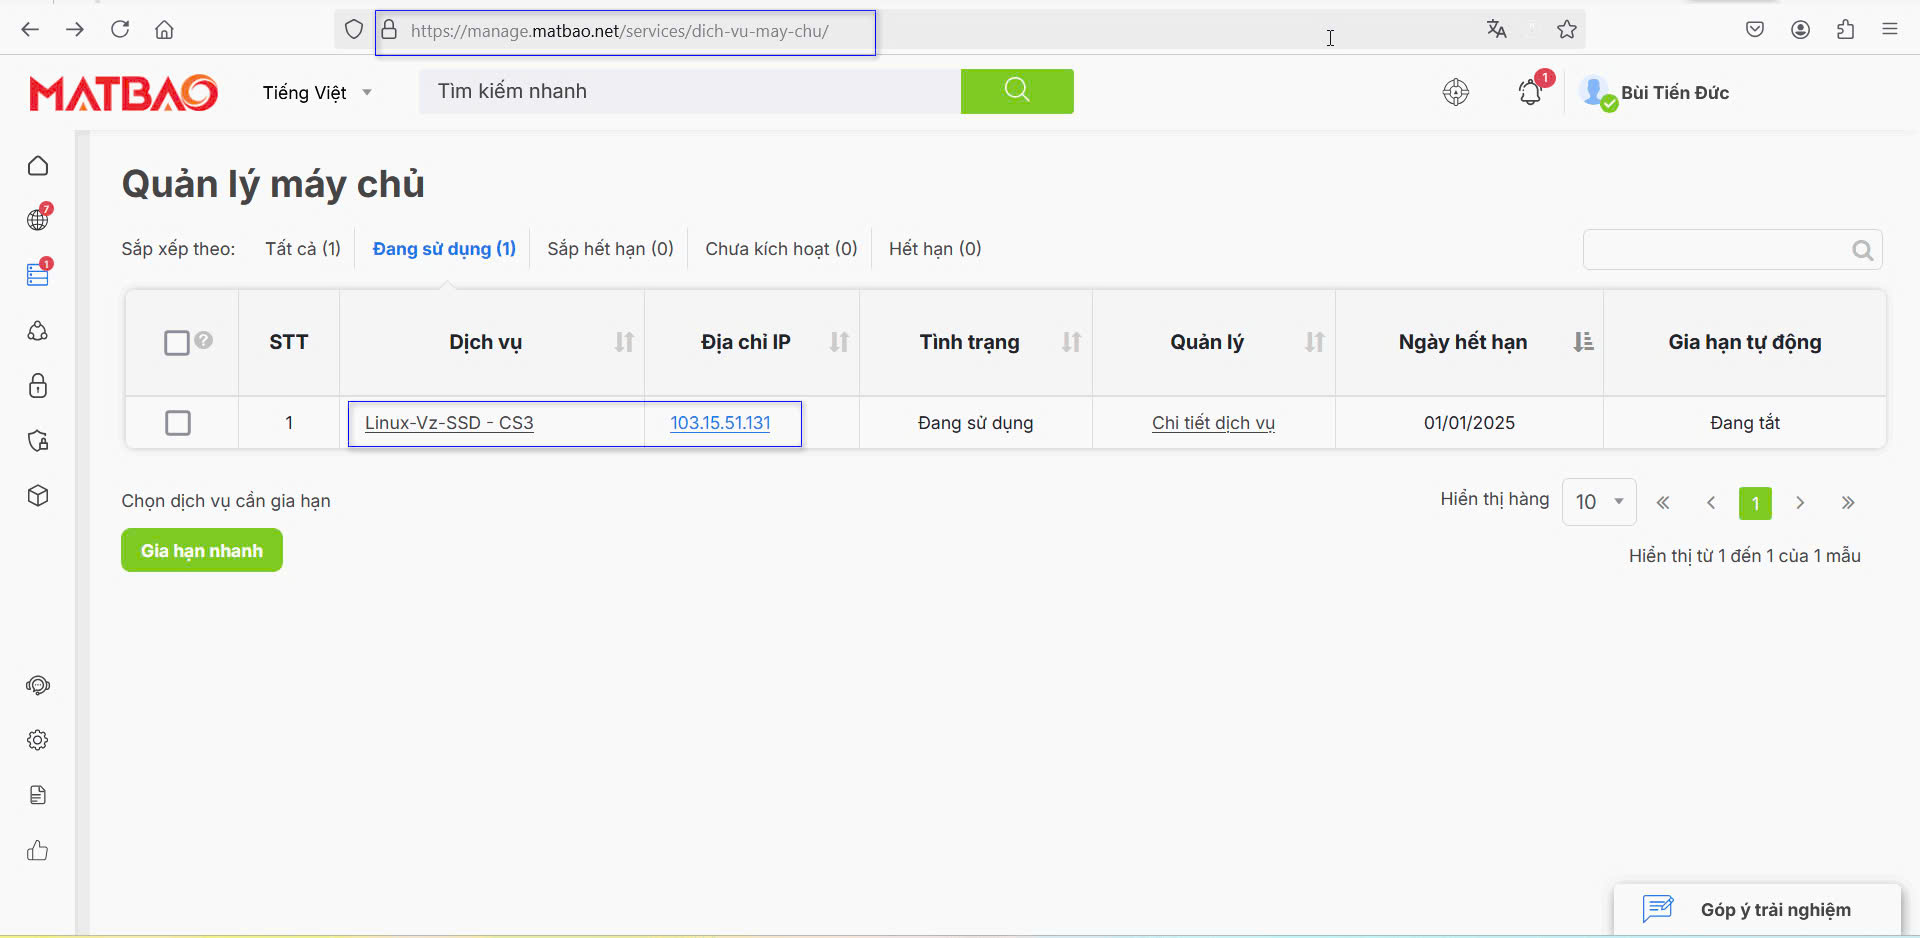
\includegraphics[width=0.8\linewidth]{images/vps4.jpg}
    \vspace{0.5cm}
    \caption{Giao diện thuê VPS}    
\end{figure}

\begin{figure}[H]
    \centering
    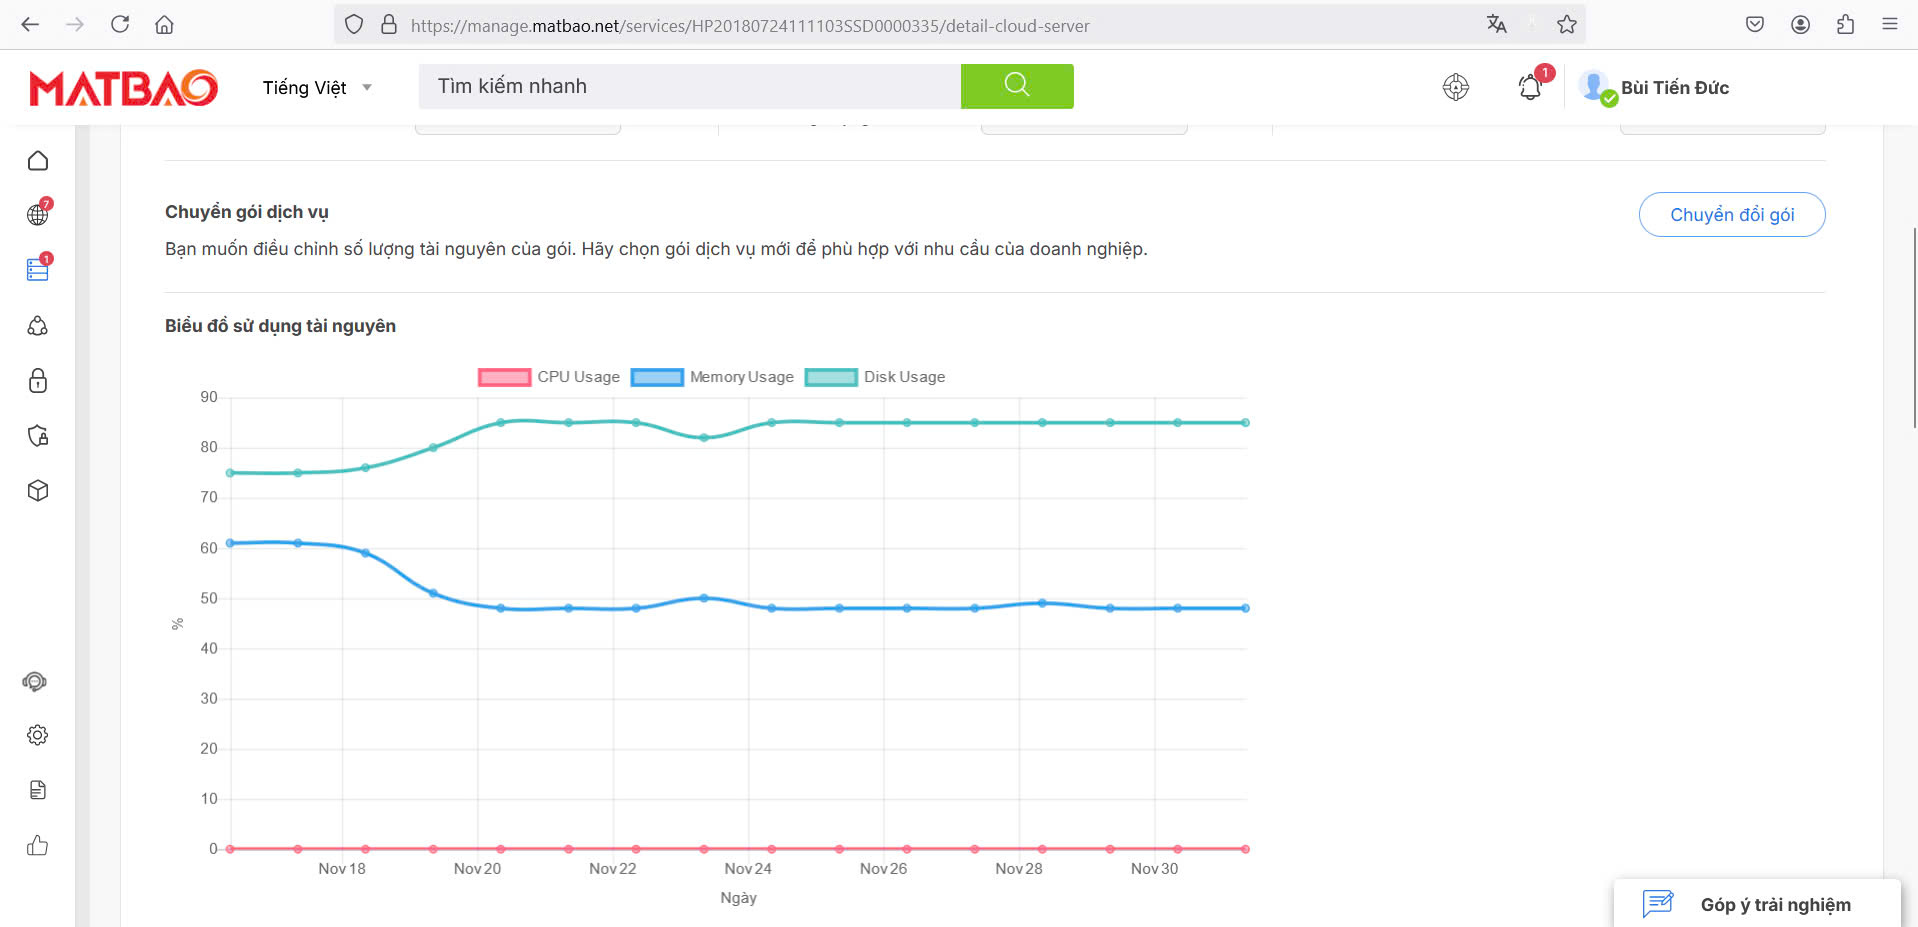
\includegraphics[width=0.8\linewidth]{images/vps2.jpg}
    \vspace{0.5cm} 
    \caption{Biểu đồ sử dụng tài nguyên}    
\end{figure}

\begin{figure}[H]
    \centering
    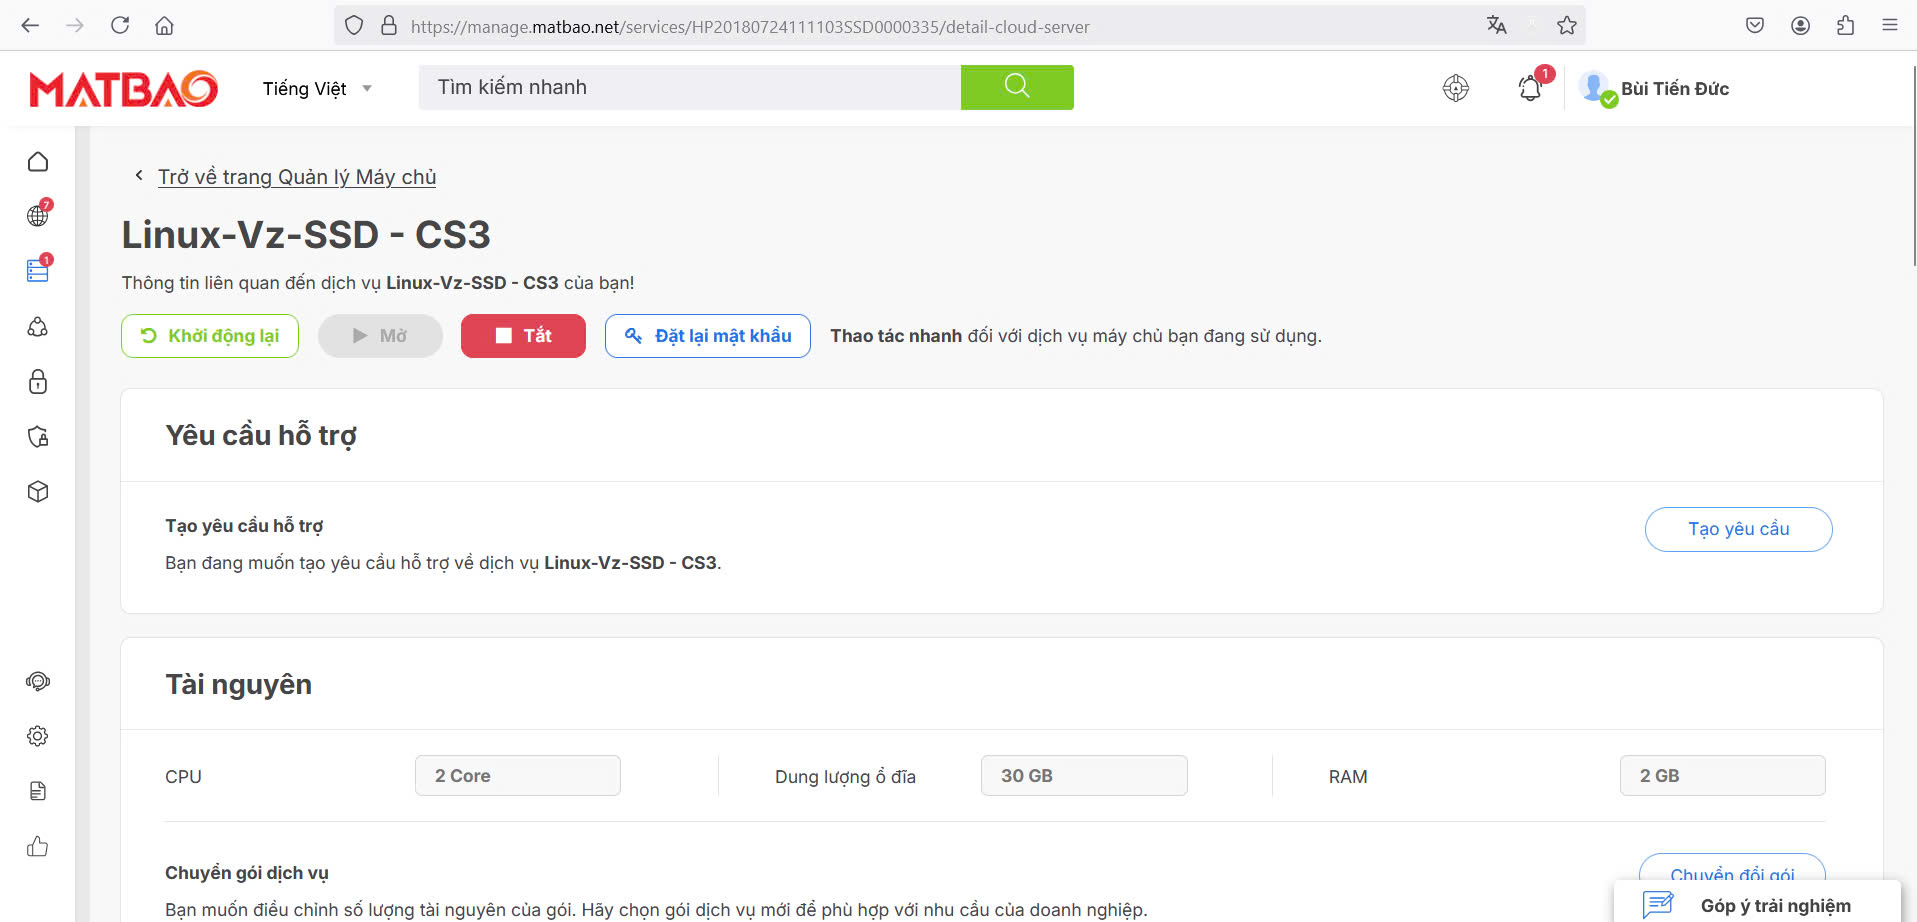
\includegraphics[width=0.8\linewidth]{images/vps3.jpg}
    \vspace{0.5cm} 
    \caption{Yêu cầu về tài nguyên}    
\end{figure}


\subsubsection{Bước 2: Truy cập VPS}
Nhóm sử dụng công cụ \textit{VSCode Studio} kết hợp với tiện ích \textit{Remote SSH} để kết nối tới máy chủ. Sau khi cấu hình SSH bằng tên đăng nhập và mật khẩu được cung cấp, có thể truy cập và làm việc trên VPS từ xa. Đây là môi trường làm việc chính cho việc triển khai hệ thống.

\subsubsection{Bước 3: Cài đặt môi trường trên VPS}
Trên hệ điều hành Linux của máy chủ, các thư viện và công cụ cần thiết được cài đặt bằng các lệnh sau:
\begin{itemize}
    \item \textbf{Cài đặt Git:} \texttt{sudo apt install git}
    \item \textbf{Cài đặt Python:} \texttt{sudo apt install python3}
    \item \textbf{Cài đặt Node.js:} Sử dụng \textit{Fast Node Manager (FNM)} để cài đặt phiên bản Node.js cụ thể và kiểm tra tính tương thích:
    \begin{verbatim}
curl -fsSL https://fnm.vercel.app/install | bash
source ~/.bashrc
fnm use --install-if-missing 22
node -v
npm -v
    \end{verbatim}
    \item \textbf{Cài đặt Docker:} Dùng các lệnh dưới đây để thiết lập Docker:
    \begin{verbatim}
sudo apt install ca-certificates curl gnupg lsb-release
sudo mkdir -p /etc/apt/keyrings
curl -fsSL https://download.docker.com/linux/ubuntu/gpg | 
    sudo gpg --dearmor -o /etc/apt/keyrings/docker.gpg
echo "deb [arch=$(dpkg --architecture -q)] 
    https://download.docker.com/linux/ubuntu $(lsb_release -cs) stable" | 
    sudo tee /etc/apt/sources.list.d/docker.list > /dev/null
sudo apt install docker-ce
    \end{verbatim}
    \item \textbf{Cài đặt Apache2:} \texttt{sudo apt install apache2}
\end{itemize}

\subsubsection{Bước 4: Khởi tạo ứng dụng}
Ứng dụng được sao chép từ GitHub bằng lệnh \texttt{git clone}. Sau đó, Docker được sử dụng để triển khai:
\begin{verbatim}
docker build -t myreactapp .
docker run -d -p 6789:6789 myreactapp
\end{verbatim}

\begin{figure}[H]
    \centering
    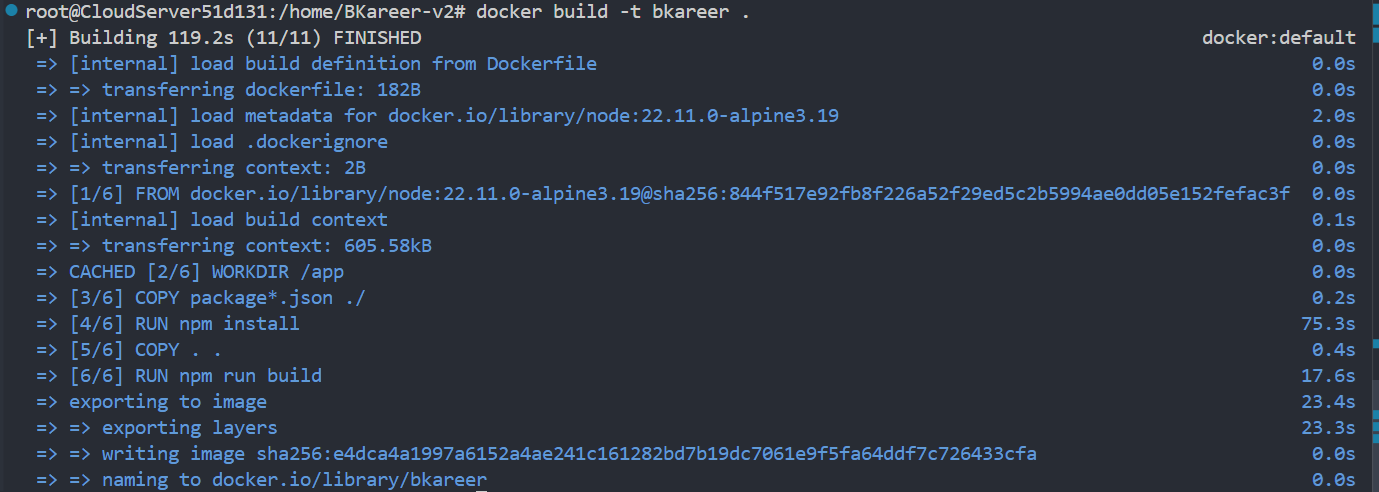
\includegraphics[width=0.9\linewidth]{images/docker build.png}
    \vspace{0.5cm}
    \caption{Triển khai ứng dụng trên Docker}
\end{figure}

Khi Docker container hoạt động, ứng dụng có thể truy cập tại cổng đã định cấu hình. Đối với nhóm là địa chỉ ip 103.15.51.131

\subsubsection{Bước 5: Đăng ký tên miền}
Nhóm đã đăng ký tên miền tại \textit{tenten.vn}. 
\begin{figure}[H]
    \centering
    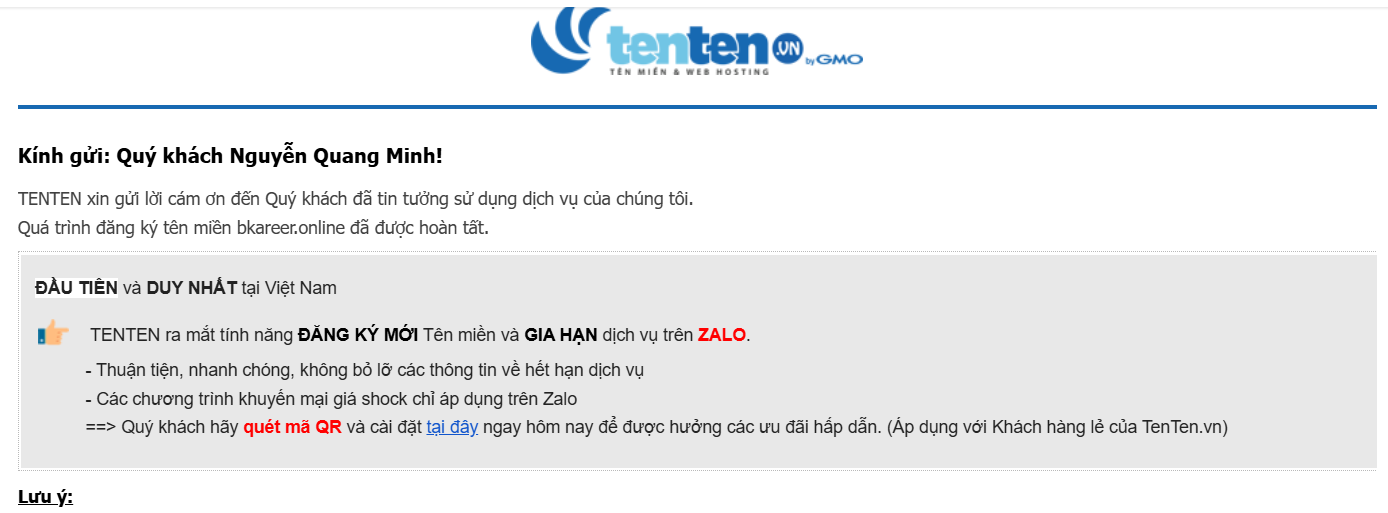
\includegraphics[width=0.9\linewidth]{images/domain.png}
    \vspace{0.5cm}
    \caption{Đăng ký tên miền}
\end{figure}    
Thiết lập DNS cho tên miền để trỏ tới địa chỉ IP của VPS.
\begin{figure}[H]
    \centering
    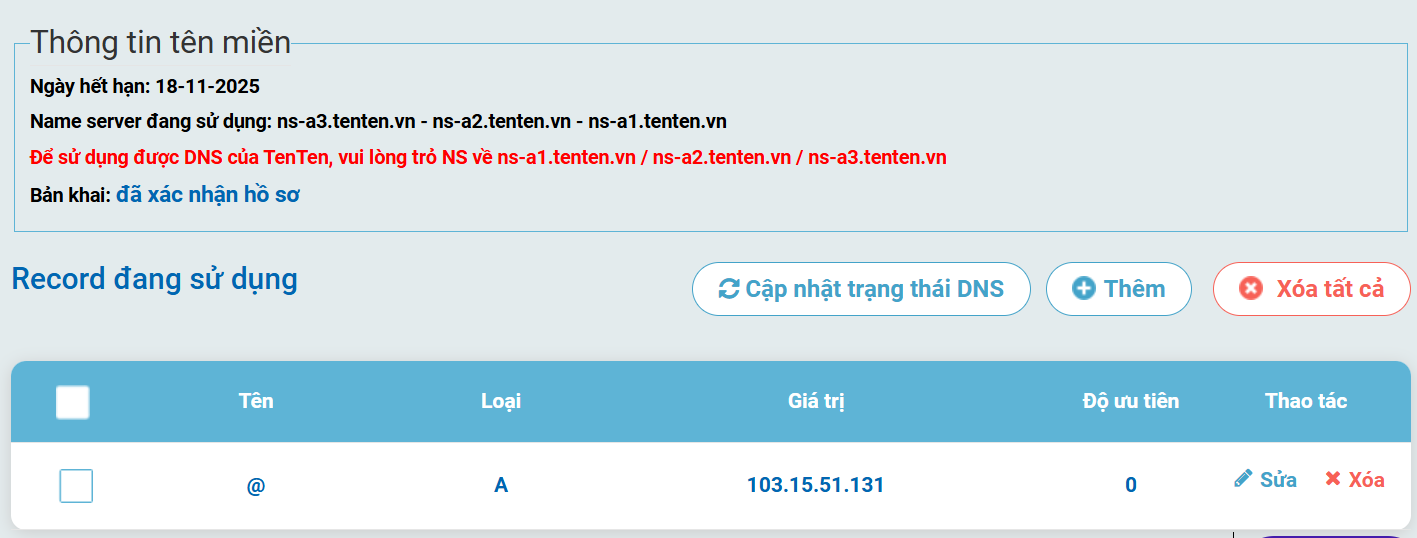
\includegraphics[width=0.9\linewidth]{images/dns.png}
    \vspace{0.5cm}
    \caption{Thiết lập DNS}
\end{figure}


Sau khi thanh toán, tên miền này được dùng để trỏ tới ứng dụng thông qua cấu hình Apache.

\subsubsection{Bước 6: Cấu hình Apache để ánh xạ tên miền}
Một cấu hình mới được tạo tại \texttt{/etc/apache2/sites-available/myproxy.conf}:
\begin{verbatim}
<VirtualHost *:80>
    ServerName yourdomain.com
    ProxyPreserveHost On
    ProxyPass / http://localhost:8080/
    ProxyPassReverse / http://localhost:8080/
    ErrorLog ${APACHE_LOG_DIR}/error.log
    CustomLog ${APACHE_LOG_DIR}/access.log combined
</VirtualHost>
\end{verbatim}

\begin{figure}[H]
    \centering
    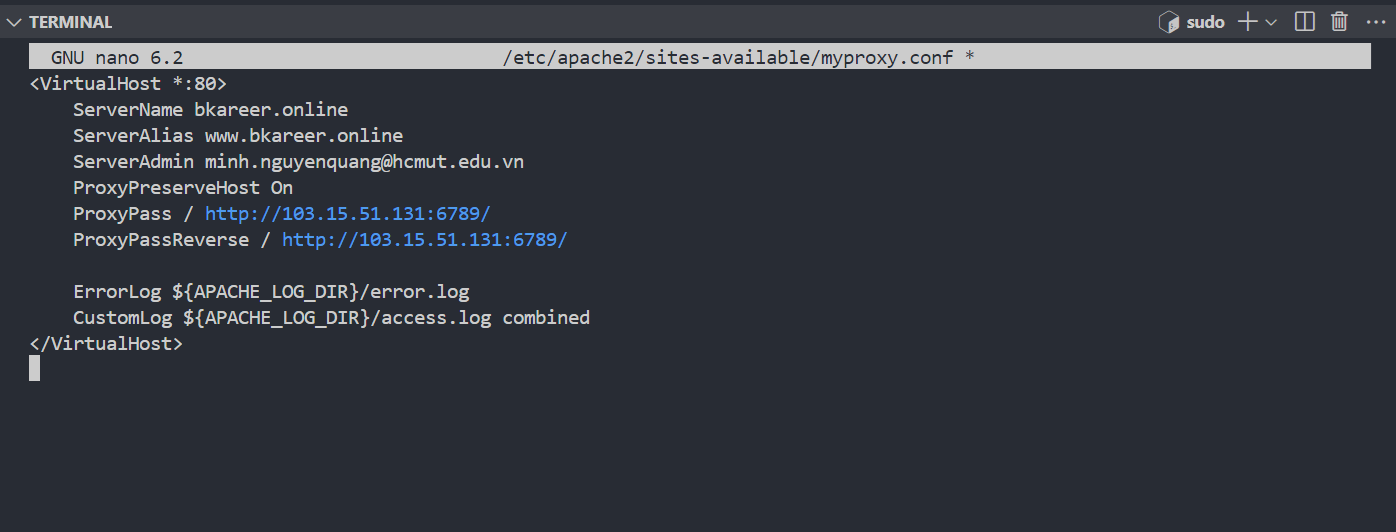
\includegraphics[width=0.9\linewidth]{images/apache-file.png}
    \vspace{0.5cm}
    \caption{Hình trên mô tả quy trình cấu hình Apache trên terminal}
\end{figure}

Sau khi kích hoạt cấu hình này (\texttt{sudo a2ensite myproxy.conf}), nhóm kiểm tra và khởi động lại Apache (\texttt{sudo apache2ctl configtest} và \texttt{sudo systemctl restart apache2}).

\begin{figure}[H]
    \centering
    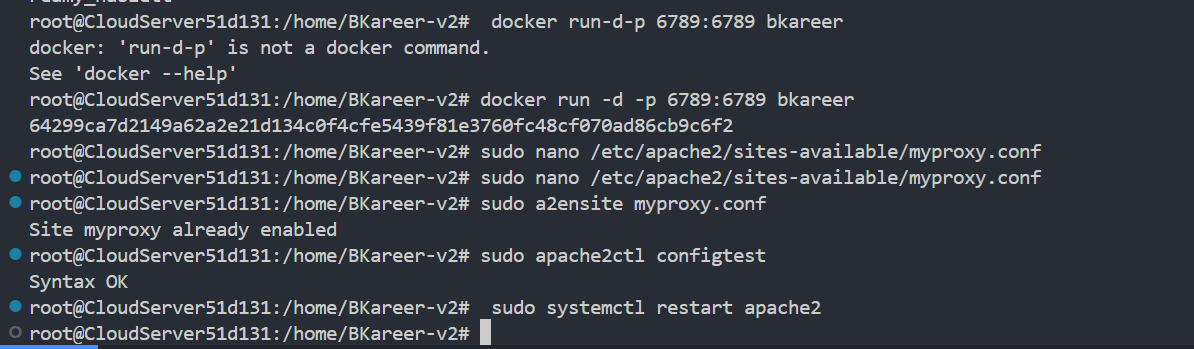
\includegraphics[width=0.9\linewidth]{images/run-docker-apache.png}
    \vspace{0.5cm}
    \caption{Hình trên mô tả quy trình khởi động lại apache sau khi kích hoạt cấu hình myproxy}
\end{figure}

\subsection{Kết quả triển khai}
Hệ thống đã được triển khai thành công, hoạt động ổn định trên tên miền \textit{bkareer.online}, với đầy đủ chức năng theo yêu cầu.


%%%%%%%%%%%%%%%%%%%%%%%%%%%% User Interface %%%%%%%%%%%%%%%%%%%%%%%%%%%%
\section{Giao diện người dùng}
%%%%%%%%%% Login Screen %%%%%%%%%%
\subsection{Trang đăng nhập}
Trang đăng nhập cho phép người dùng nhập thông tin đăng nhập, xác thực danh tính, sau khi thành công sẽ chuyển hướng đến trang chủ.

Trang đăng nhập được thiết kế với giao diện đơn giản, trực quan, tập trung vào hai trường nhập liệu chính là ``Email" và ``Mật khẩu", phía dưới trường nhập liệu ``Mật khẩu" là liên kết ``Quên mật khẩu". Nút ``Đăng nhập" và ``Đăng nhập với Google" được đặt ở vị trí nổi bật. Cuối trang có lựa chọn chuyển đến trang đăng ký tài khoản cho người dùng mới sử dụng hệ thống.

Mục đích của trang đăng nhập:
\begin{itemize}
    \item Xác thực danh tính: Đảm bảo rằng chỉ những người có quyền truy cập mới được vào hệ thống.
    \item Bảo mật thông tin: Bảo vệ dữ liệu cá nhân của người dùng khỏi sự truy cập trái phép.
    \item Tạo trải nghiệm người dùng tốt: Một trang đăng nhập thân thiện, dễ sử dụng sẽ giúp người dùng có ấn tượng tốt về website.
\end{itemize}

\begin{figure}[H]
    \centering
    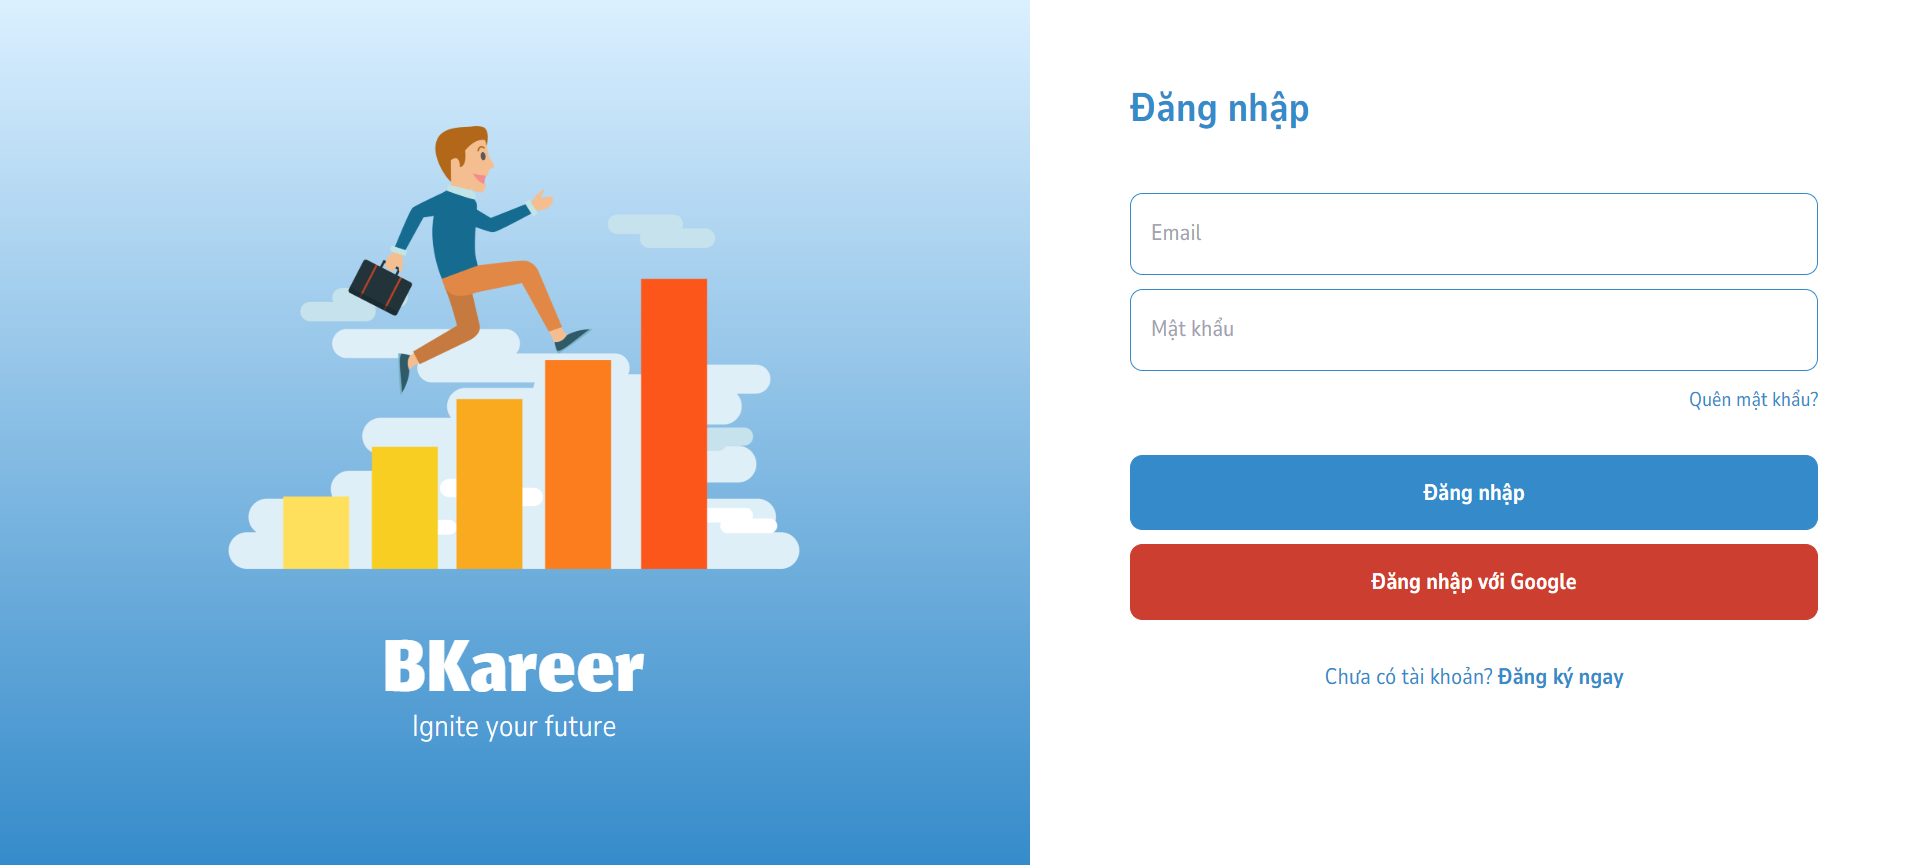
\includegraphics[width=0.8\linewidth]{images/chap5/login.png}
    \vspace{0.5cm}
    \caption{Trang đăng nhập}
\end{figure}

Các thành phần chính của trang đăng nhập:
\begin{itemize}
    \item Các trường nhập liệu:
        \begin{itemize}
            \item Email: Ô nhập liệu cho người dùng nhập tên đăng nhập.
            \item Mật khẩu: Ô nhập liệu cho người dùng nhập mật khẩu.
        \end{itemize}
    \item Nút:
        \begin{itemize}
            \item Nút ``Quên mật khẩu": Liên kết đến trang phục hồi mật khẩu.
            \item Nút ``Đăng nhập": Nút bấm để xác thực thông tin đăng nhập.
            \item Nút ``Đăng nhập với Google": Cho phép người dùng sử dụng trực tiếp tài khoản Google đã có sẵn của họ để đăng nhập.
            \item Nút ``Đăng ký ngay": Chuyển hướng đến trang đăng ký, cho phép người dùng mới tạo tài khoản cá nhân.
        \end{itemize}
    \item Các thành phần khác:
        \begin{itemize}
            \item Thông báo lỗi: Hiển thị khi thông tin đăng nhập không chính xác.
        \end{itemize}
\end{itemize}


%%%%%%%%%% Register Screen %%%%%%%%%%
\subsection{Trang đăng ký}
Trang đăng ký là một phần không thể thiếu trong hầu hết các ứng dụng. Nó đóng vai trò quan trọng trong việc thu thập thông tin người dùng, xây dựng cơ sở dữ liệu khách hàng và tạo ra tài khoản cá nhân cho từng người.

Trang đăng ký được thiết kế với giao diện đơn giản, trực quan, tập trung vào ba trường nhập liệu chính là ``Tên người dùng", ``Email" và ``Mật khẩu". Nút ``Đăng ký" và ``Đăng nhập với Google" được đặt ở vị trí nổi bật. Cuối trang có lựa chọn chuyển đến trang đăng nhập cho người dùng đã có tài khoản đăng nhập vào hệ thống.

Mục đích của trang đăng ký:
\begin{itemize}
    \item Thu thập thông tin người dùng: Tên, email, số điện thoại, ngày sinh, giới tính...
    \item Xây dựng cơ sở dữ liệu khách hàng: Tạo danh sách người dùng để phục vụ cho các hoạt động marketing, hỗ trợ khách hàng.
    \item Tạo tài khoản cá nhân: Cho phép người dùng truy cập vào các tính năng và dịch vụ riêng tư.
\end{itemize}

\begin{figure}[H]
    \centering
    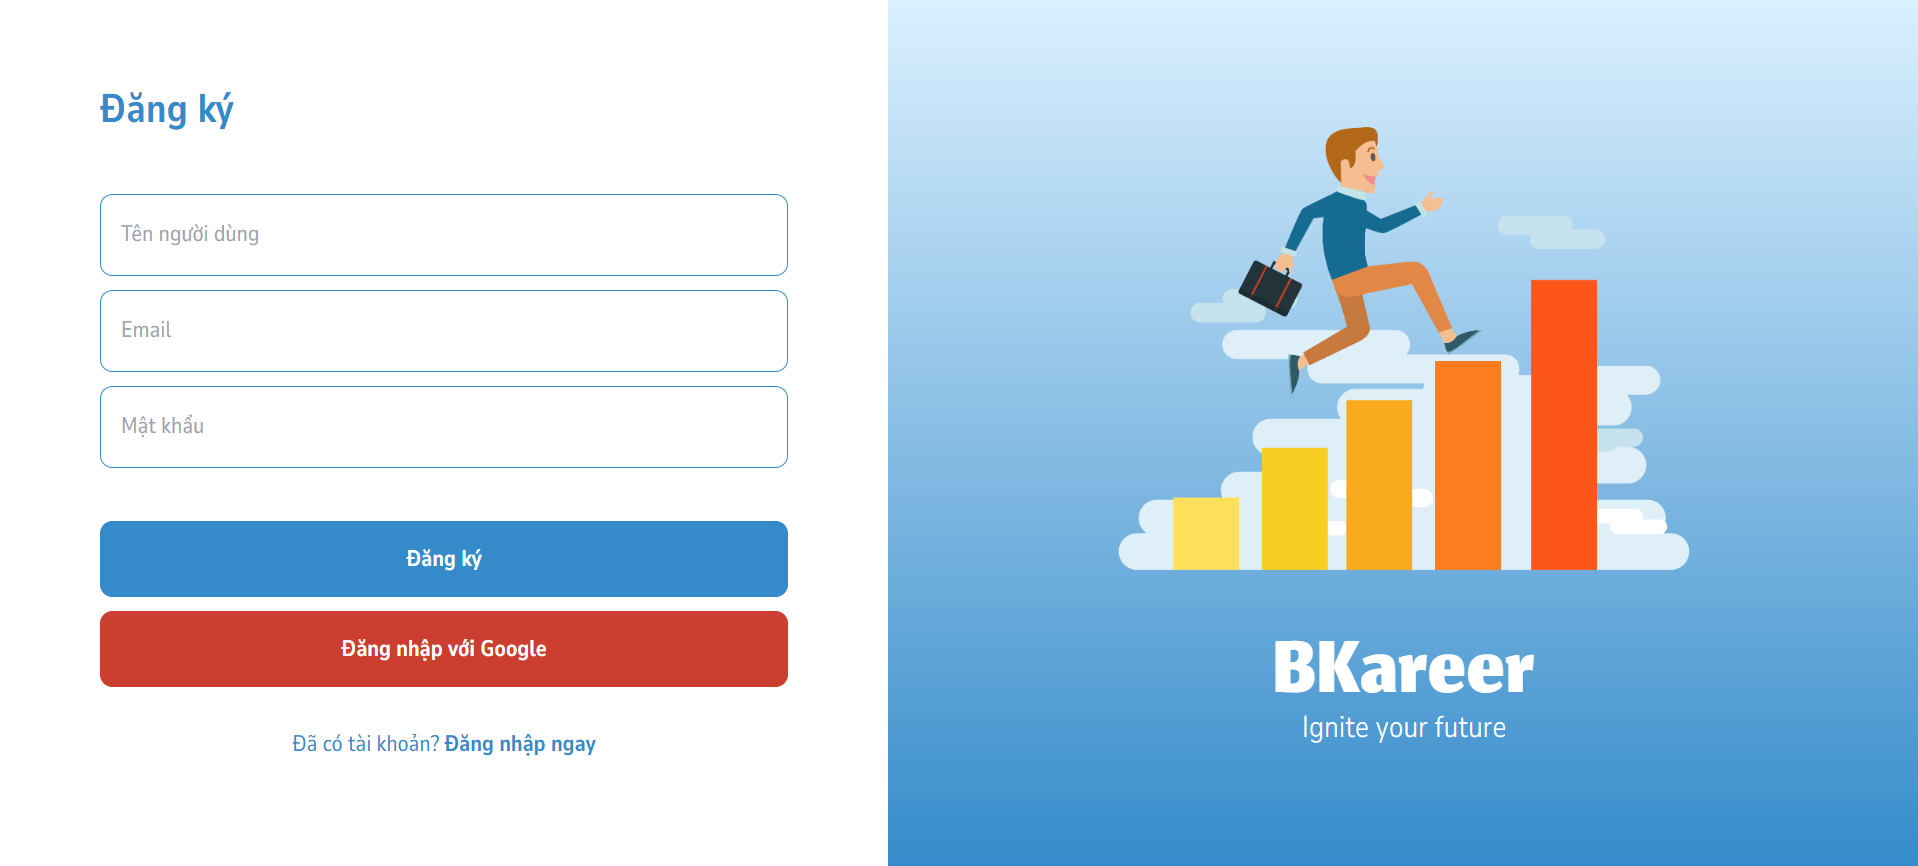
\includegraphics[width=0.8\linewidth]{images/chap5/register.png}
    \vspace{0.5cm}
    \caption{Trang đăng ký}
\end{figure}

Các thành phần chính của trang đăng ký:
\begin{itemize}
    \item Các trường nhập liệu:
        \begin{itemize}
            \item Tên người dùng: Ô nhập liệu cho người dùng tên người dùng hiển thị trong hệ thống.
            \item Email: Ô nhập liệu cho người dùng nhập tên đăng nhập.
            \item Mật khẩu: Ô nhập liệu cho người dùng nhập mật khẩu.
        \end{itemize}
    \item Nút:
        \begin{itemize}
            \item Nút ``Đăng ký": Cho phép người dùng tạo tài khoản mới và bắt đầu sử dụng hệ thống.
            \item Nút ``Đăng nhập với Google": Cho phép người dùng sử dụng trực tiếp tài khoản Google đã có sẵn của họ để đăng nhập.
            \item Nút ``Đăng nhập ngay": Chuyển hướng đến trang đăng nhập, cho phép người dùng đăng nhập vào hệ thống.
        \end{itemize}
    \item Các thành phần khác:
        \begin{itemize}
            \item Thông báo lỗi: Hiển thị khi thông tin đăng nhập không chính xác.
        \end{itemize}
\end{itemize}


%%%%%%%%%% Home Screen %%%%%%%%%%
\subsection{Trang chủ}
Trang chủ là cửa ngõ đầu tiên của người dùng khi truy cập vào một website. Nó đóng vai trò quan trọng trong việc tạo ấn tượng ban đầu, truyền tải thông điệp của thương hiệu và hướng người dùng đến các mục tiêu cụ thể.

Trang chủ của BKareer được thiết kế với giao diện hiện đại, thân thiện với người dùng. Màu sắc chủ đạo là xanh dương và trắng, tạo cảm giác tin cậy và chuyên nghiệp. Bố cục trang được chia thành các khối rõ ràng, giúp người dùng dễ dàng tìm kiếm thông tin cần thiết.

Mục đích của trang chủ:
\begin{itemize}
    \item Giới thiệu tổng quan: Trang chủ là nơi để giới thiệu ngắn gọn, súc tích về hệ thống.
    \item Thu hút sự chú ý: Thiết kế bắt mắt, nội dung hấp dẫn sẽ giúp thu hút người dùng ngay từ cái nhìn đầu tiên.
    \item Hướng dẫn người dùng: Chỉ dẫn người dùng đến những thông tin họ cần tìm kiếm một cách nhanh chóng và dễ dàng.
\end{itemize}

\begin{figure}[H]
    \centering
    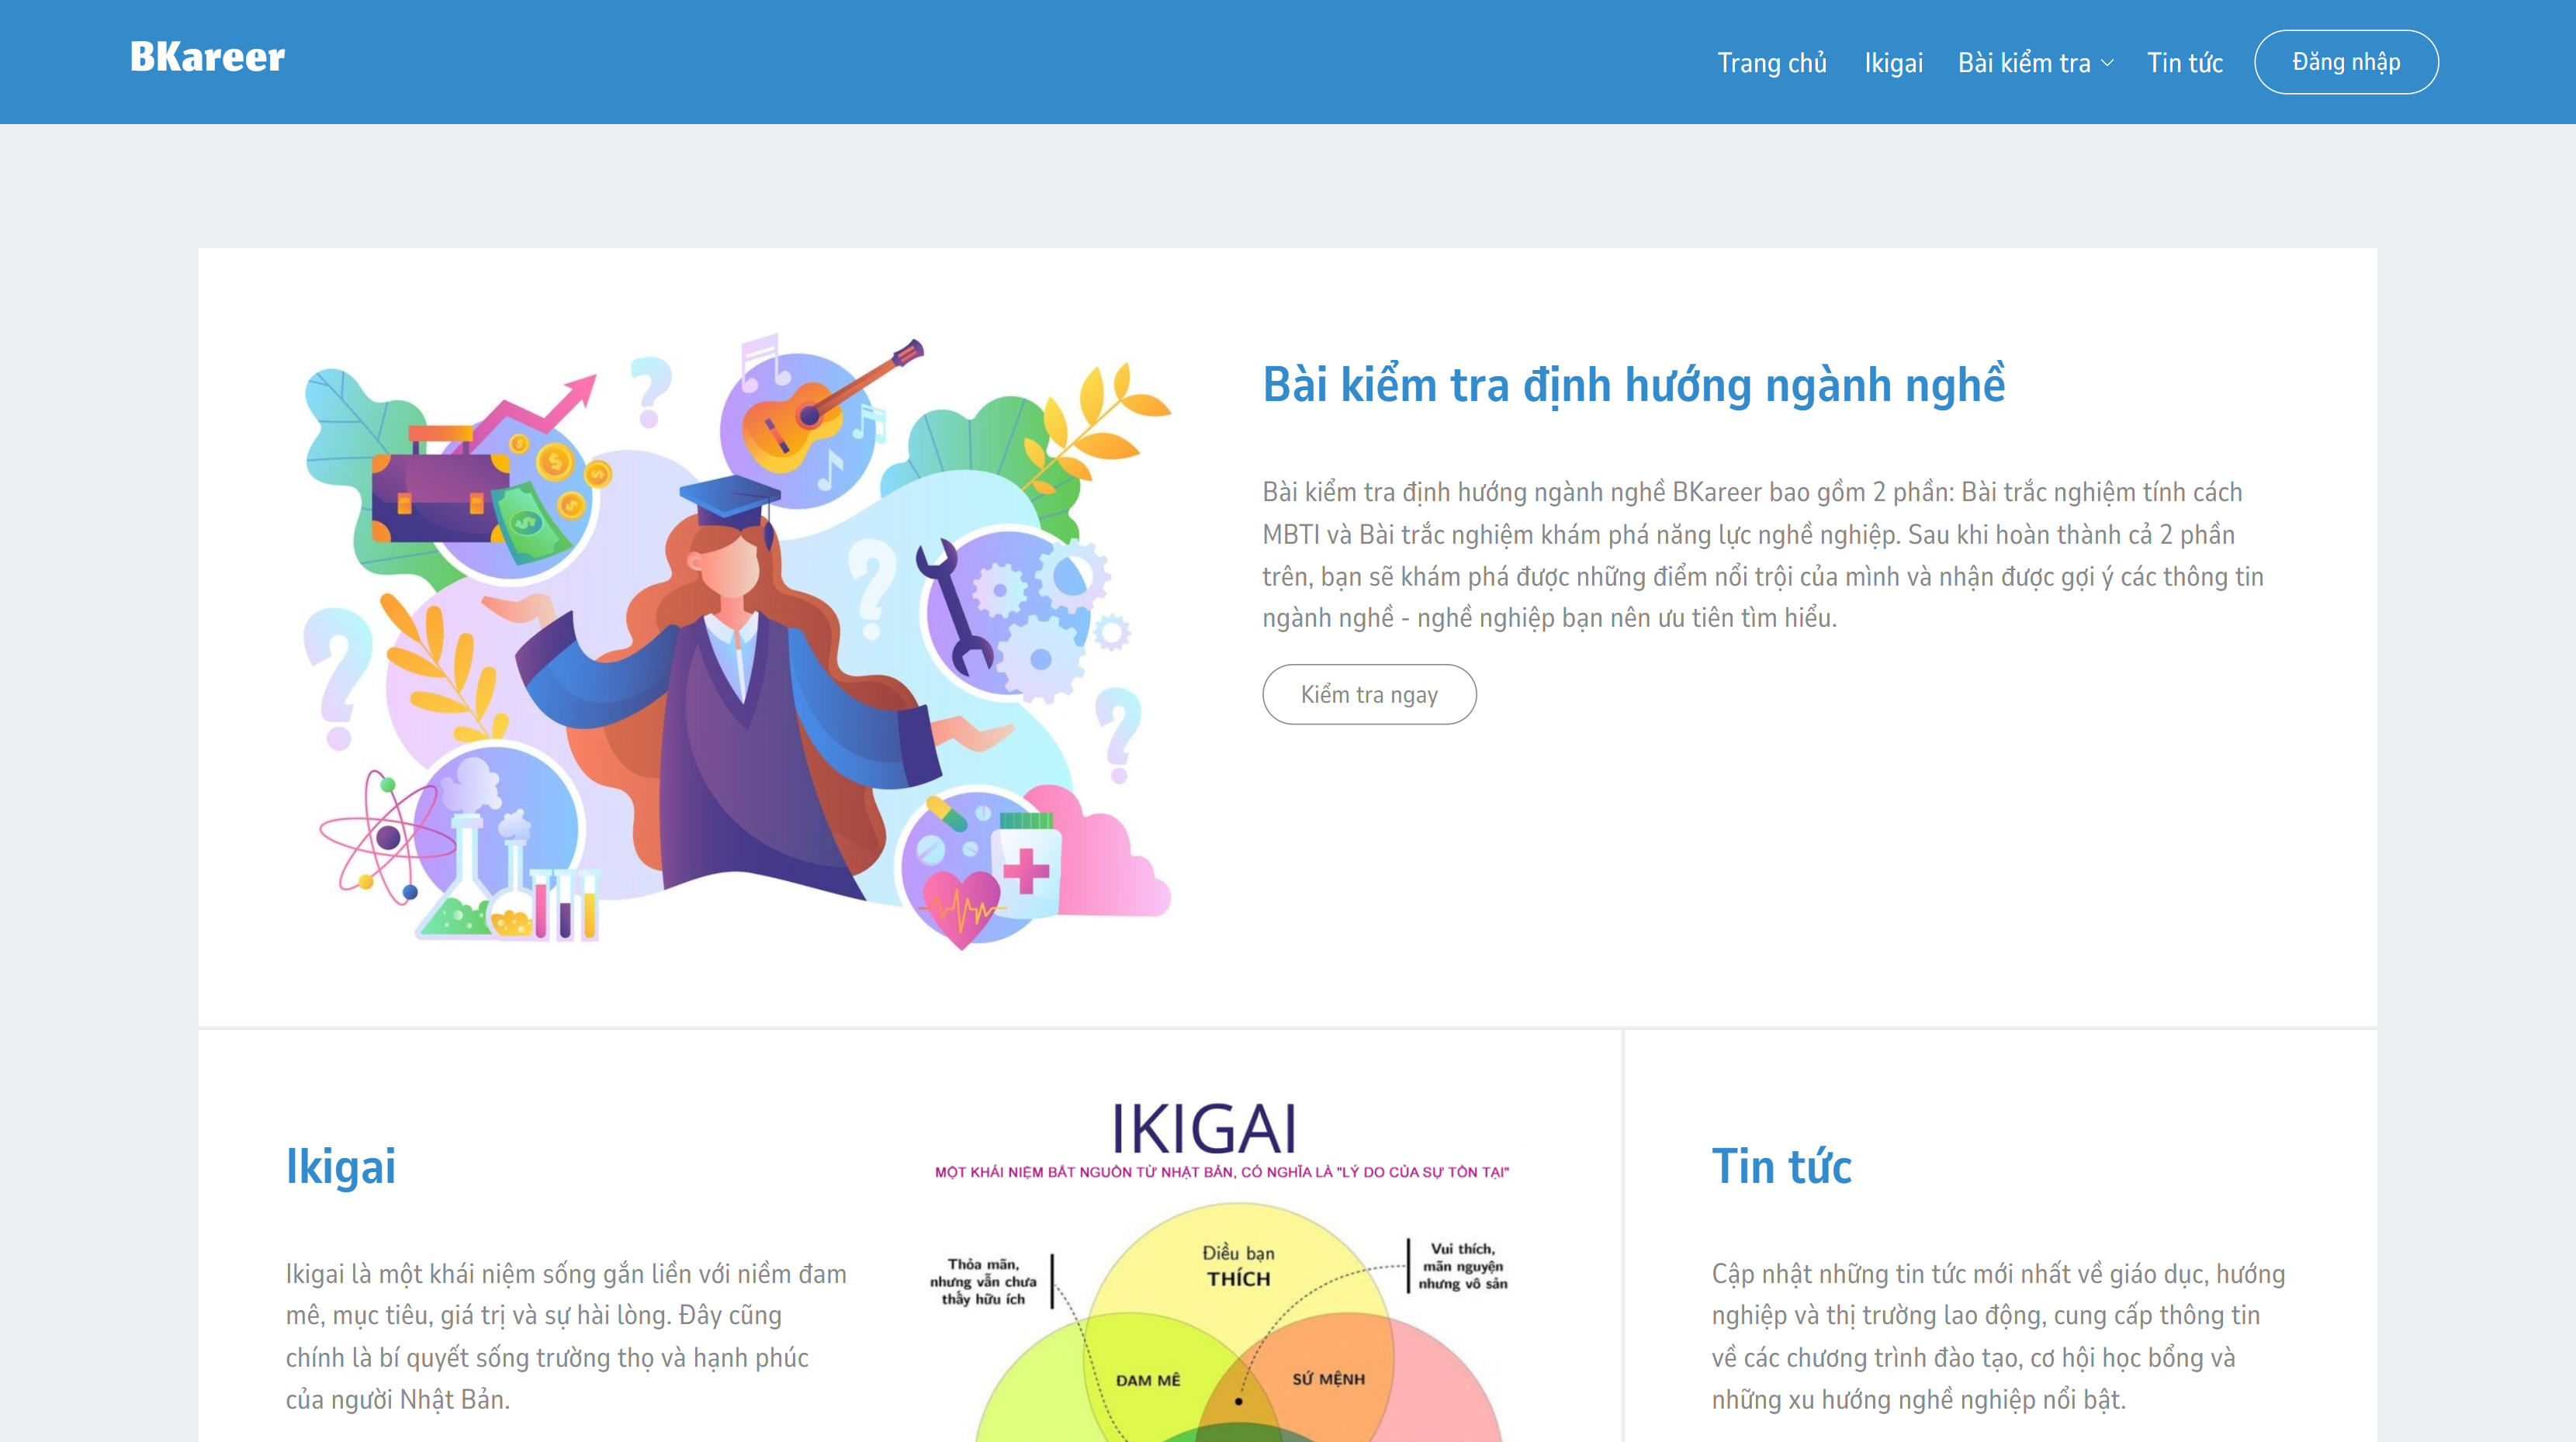
\includegraphics[width=0.8\textwidth]
    {images/chap5/homeScreen.png}
    \vspace{0.5cm}
    \caption{Trang chủ}
\end{figure}

Các thành phần chính của trang chủ:
\begin{itemize}
    \item Header: Thanh điều hướng được cố định trên cùng của trang web sẽ giúp người dùng dễ dàng tìm kiếm và di chuyển giữa các trang khác nhau, bao gồm:
        \begin{itemize}
            \item Trang chủ
            \item Trang giới thiệu về Ikigai
            \item Trình thả xuống một danh sách các bài kiểm tra được tích hợp trong hệ thống: Trắc nghiệm tính cách MBTI, Khám phá năng lực nghề nghiệp, Trắc nghiệm IQ, Trắc nghiệm EQ,...
            \item Trang tin tức
        \end{itemize}
    \item Body: Các khối thông tin được hiển thị đẹp mắt, rõ ràng giúp người dùng dễ dàng tìm kiếm và tiếp cận thông tin.
    \item Footer: Giới thiệu về đội ngũ xây dựng hệ thống, thông tin liên hệ và bản quyền hệ thống.
\end{itemize}


%%%%%%%%%% Profile Screen %%%%%%%%%%
\subsection{Trang thông tin người dùng}
Trang thông tin người dùng là một phần quan trọng của hệ thống, hiển thị thông tin chi tiết về một người dùng cụ thể. Đây là công cụ quan trọng để quản lý thông tin cá nhân, cho phép người dùng xem, chỉnh sửa và quản lý thông tin cá nhân của mình cũng như giúp hệ thống cá nhân hóa trải nghiệm người dùng.

Các thành phần chính: Các tab chuyên biệt (Tài khoản của tôi, Lịch sử thực hiện kiểm tra, Cài đặt).

Mục đích của trang thông tin người dùng:
\begin{itemize}
    \item Quản lý thông tin cá nhân: Người dùng có thể xem, cập nhật và chỉnh sửa thông tin cá nhân.
    \item Tương tác với cộng đồng: Trang thông tin người dùng cho phép người dùng chia sẻ thông tin về bản thân, kết nối với những người dùng khác và tham gia vào các hoạt động chung.
    \item Tăng cường trải nghiệm người dùng: Giúp người dùng cảm thấy được cá nhân hóa và chủ động hơn.
\end{itemize}


%%%%%%%%%% Profile - My Account Screen %%%%%%%%%%
\subsubsection{Trang tài khoản của tôi}
Trang tài khoản của tôi là một phần của hệ thống mà người dùng có thể truy cập để xem và quản lý thông tin cá nhân, cài đặt, và các hoạt động liên quan đến tài khoản của mình. Nói cách khác, đây là ``nơi ở" trực tuyến của người dùng trên một nền tảng cụ thể.

\begin{figure}[H]
    \centering
    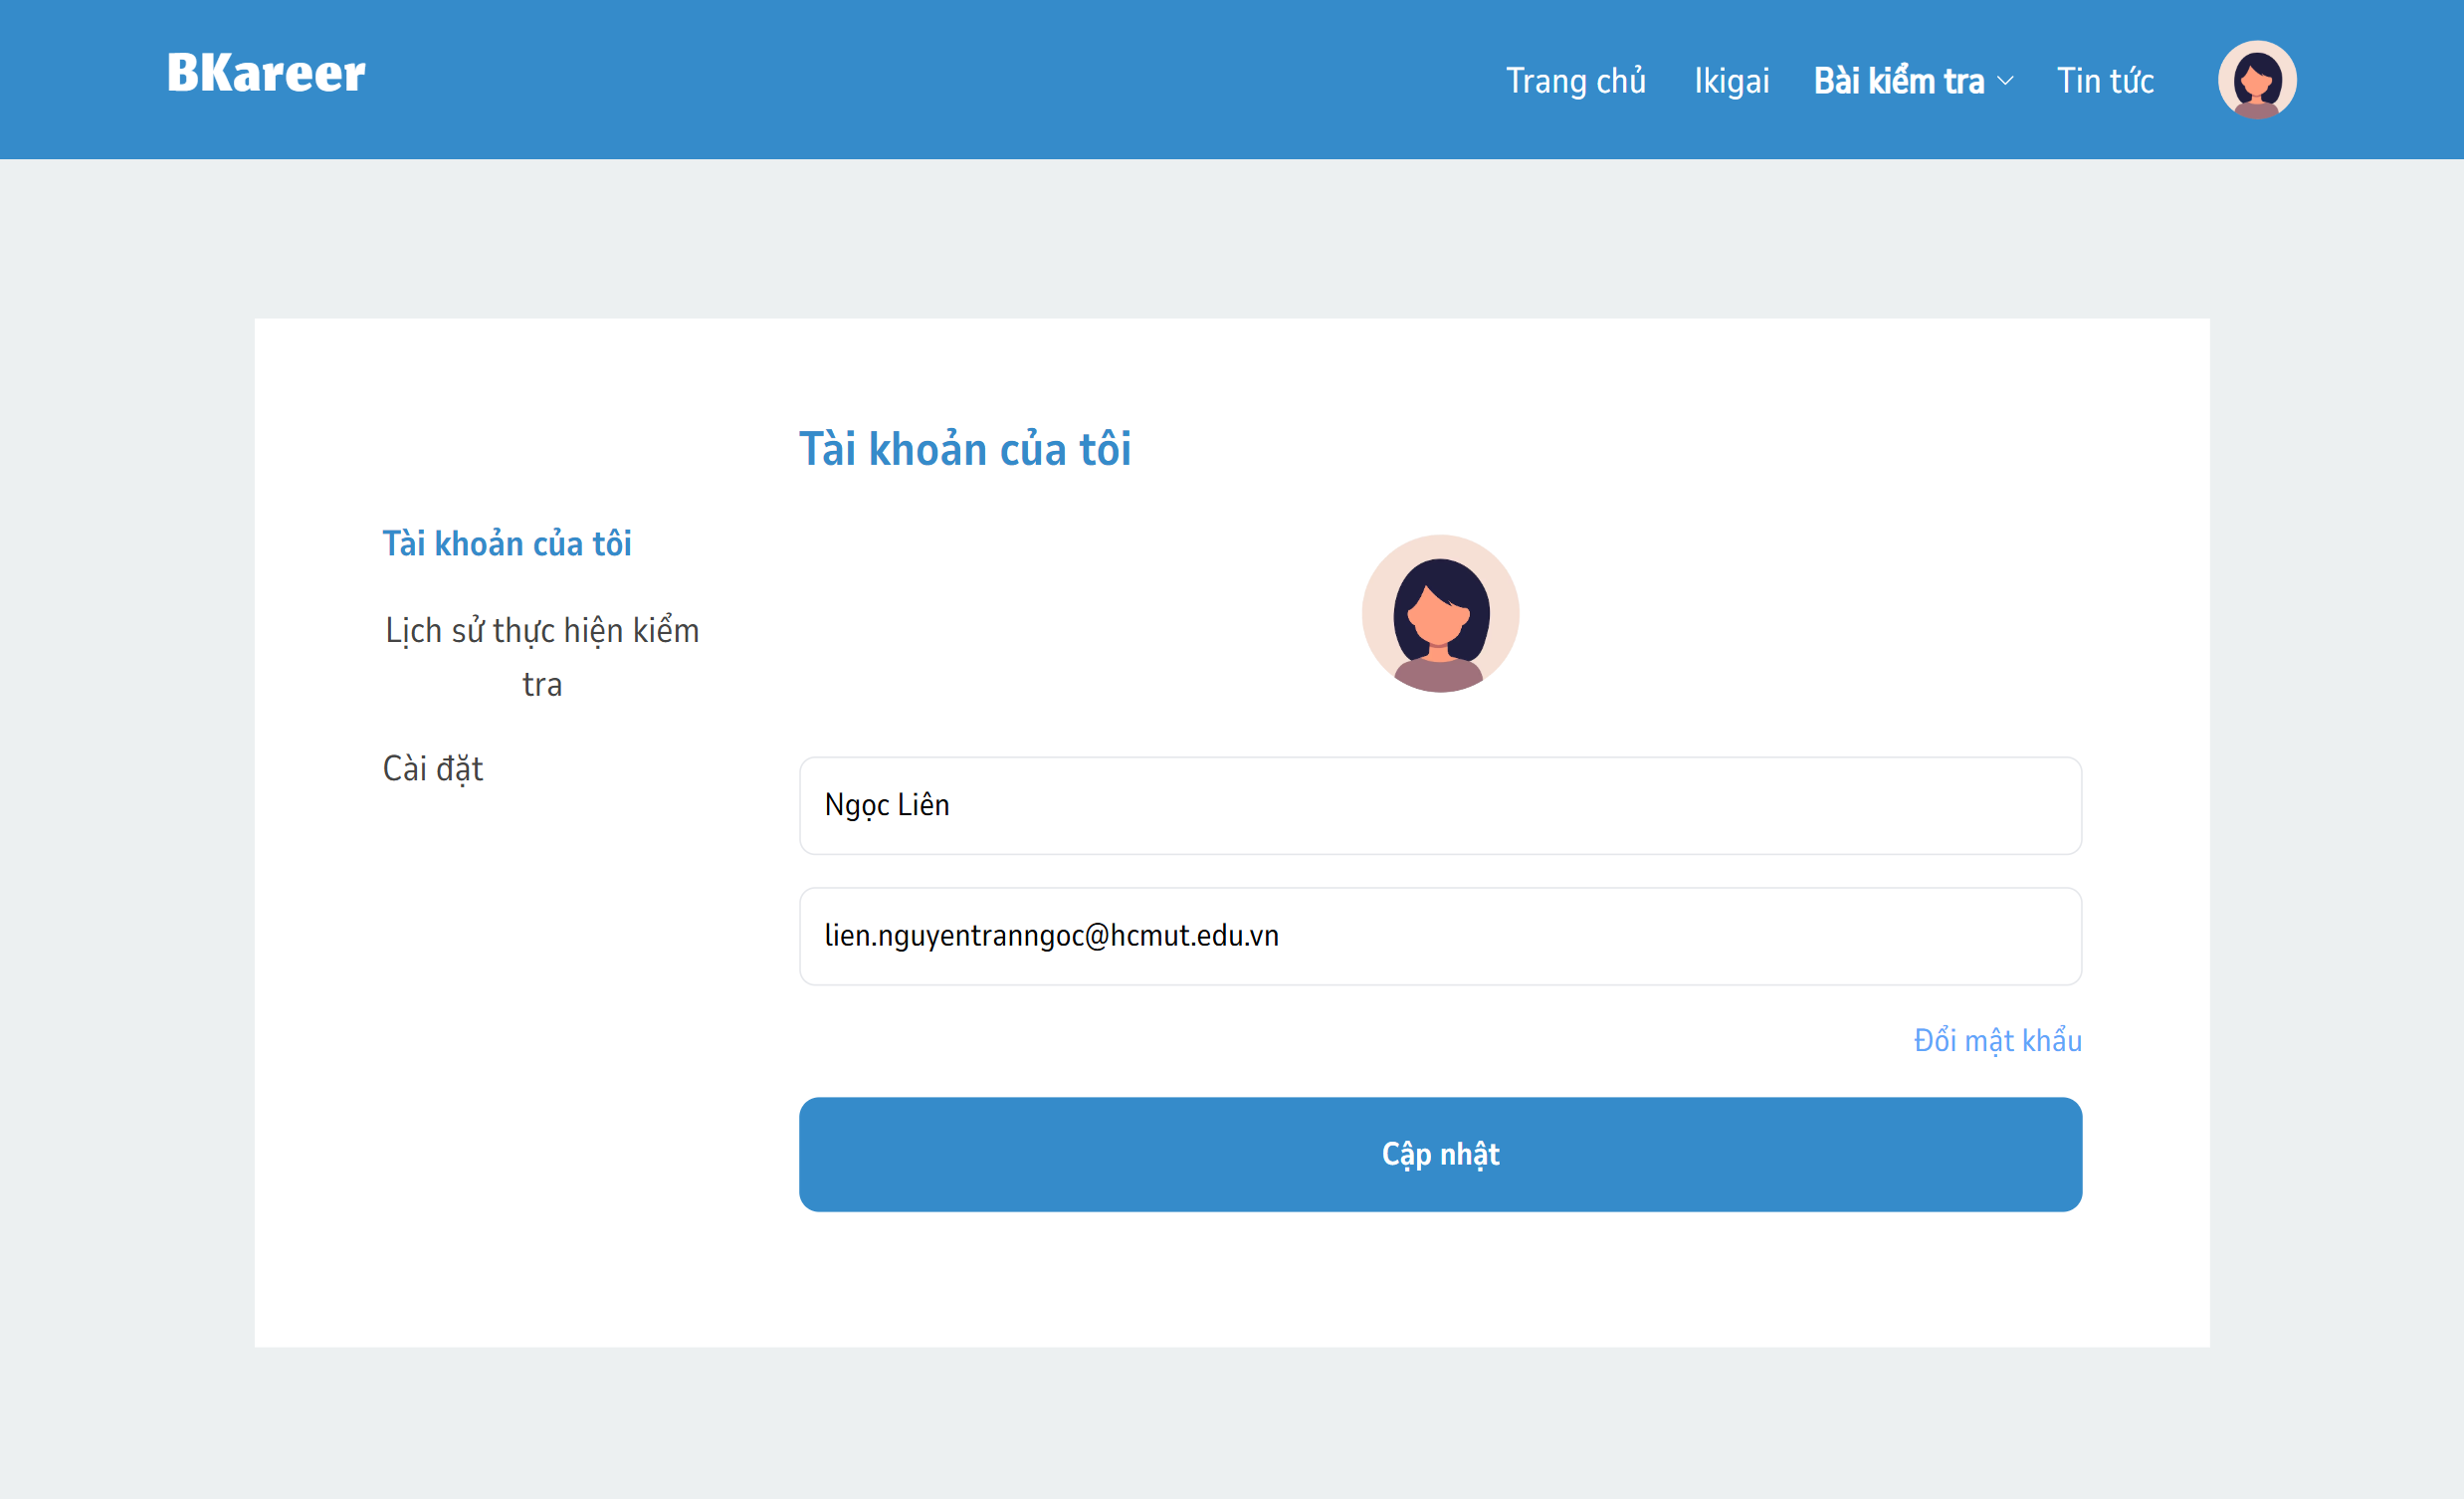
\includegraphics[width=0.8\linewidth]{images/chap5/profileScreen.png}
    \vspace{0.5cm}
    \caption{Trang tài khoản của tôi}
\end{figure}

Các thành phần chính của trang tài khoản của tôi:
\begin{itemize}
    \item Tên tab: Tên tab cung cấp thông tin sơ lược về nội dung sẽ được hiển thị trong tab đó.
    \item Ảnh đại diện: Hình ảnh đại diện của người dùng.
    \item Các trường nhập liệu:
        \begin{itemize}
            \item Tên người dùng: Hiển thị tên người dùng hiện tại và cho phép chỉnh sửa tên người dùng mới.
            \item Email: Hiển thị email hiện tại và cho phép chỉnh sửa email mới.
            \item Mật khẩu: Ô nhập liệu cho phép người dùng nhập mật khẩu mới muốn thay đổi.
        \end{itemize}
    \item Nút:
        \begin{itemize}
            \item Nút ``Cập nhật": Cho phép người dùng cập nhật thông tin cá nhân trên hệ thống.
            \item Nút ``Xóa tài khoản": Cho phép người dùng thực hiện yêu cầu xóa bỏ hoàn toàn tài khoản và tất cả dữ liệu liên quan đến tài khoản đó trên hệ thống.
            \item Nút ``Đăng xuất": Cho phép người dùng thoát khỏi tài khoản hiện tại và quay trở lại trạng thái chưa đăng nhập.
        \end{itemize}
\end{itemize}

%%%%%%%%%% Profile - Result Screen %%%%%%%%%%
\subsubsection{Trang lịch sử thực hiện kiểm tra}
Trang lịch sử thực hiện kiểm tra là một tính năng thường được tích hợp vào các hệ thống quản lý học tập, phần mềm đánh giá, hoặc các nền tảng trực tuyến khác. Nó cung cấp một bản ghi chi tiết về tất cả các hoạt động kiểm tra, đánh giá đã diễn ra trong quá khứ, giúp người dùng dễ dàng theo dõi, phân tích và đánh giá kết quả kiểm tra.

\begin{figure}[H]
    \centering
    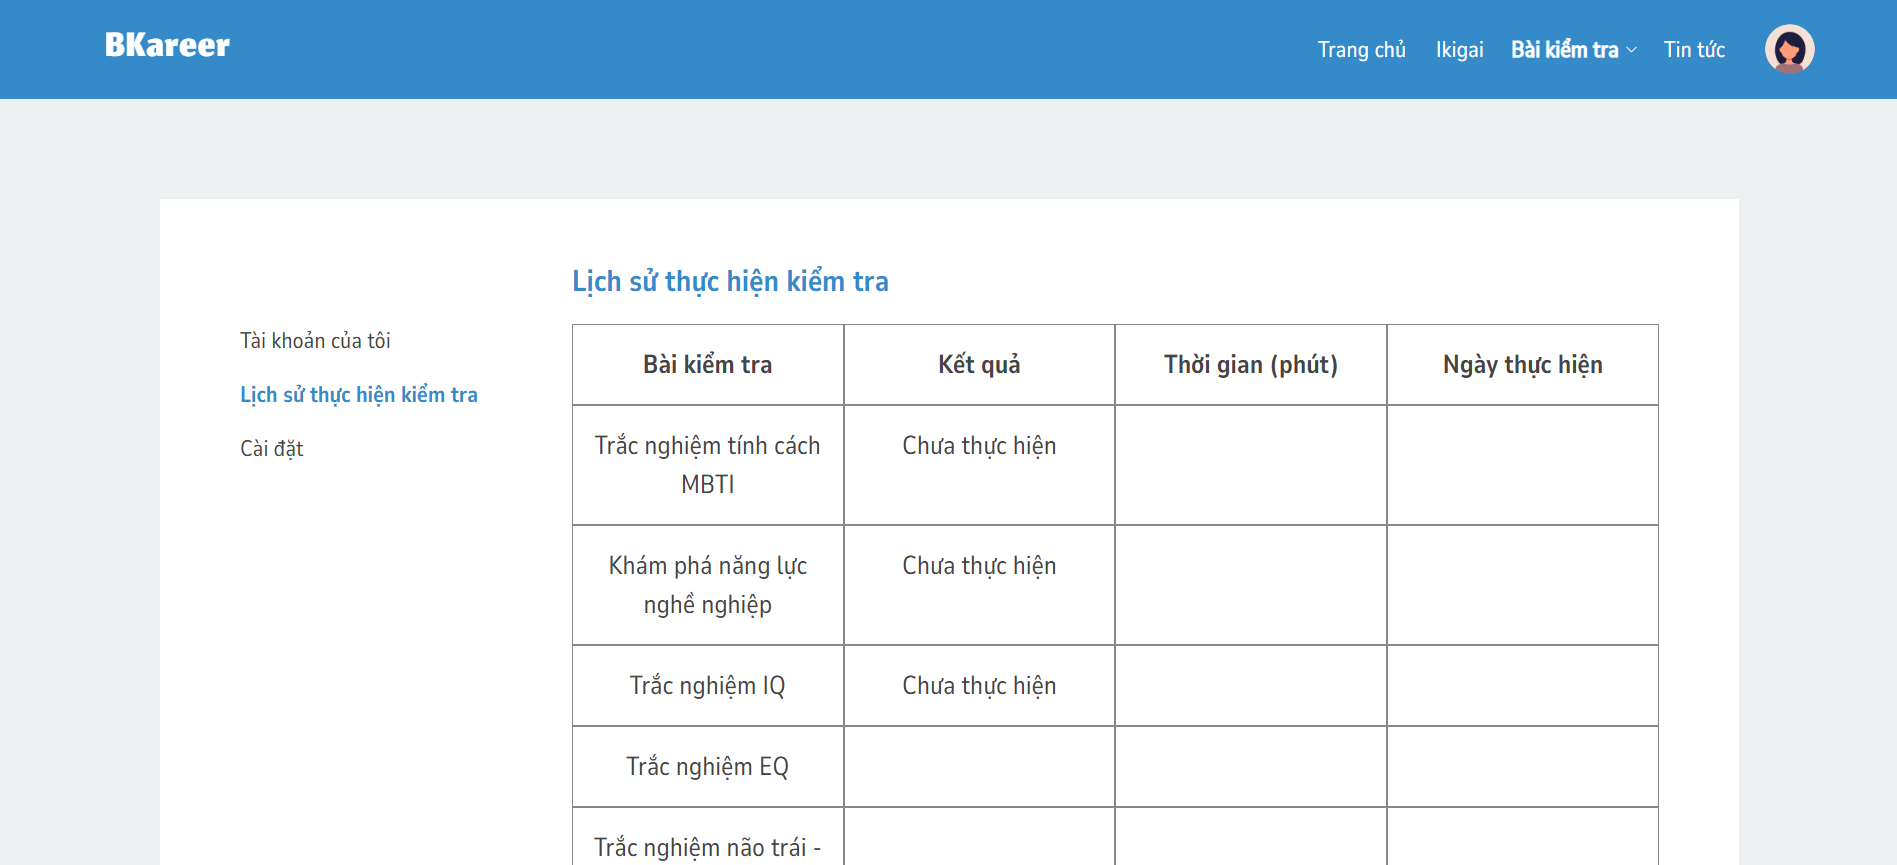
\includegraphics[width=0.8\linewidth]{images/chap5/profile-Result.png}
    \vspace{0.5cm}
    \caption{Trang lịch sử thực hiện kiểm tra}
\end{figure}

Các thành phần chính của trang lịch sử thực hiện kiểm tra:
\begin{itemize}
    \item Tên tab: Tên tab cung cấp thông tin sơ lược về nội dung sẽ được hiển thị trong tab đó.
    \item Bảng dữ liệu:
        \begin{itemize}
            \item Bài kiểm tra: Mô tả ngắn gọn, rõ ràng về tên của các bài kiểm tra.
            \item Kết quả: Thể hiện kết quả ghi nhận thực hiện các bài kiểm tra tương ứng.
            \item Thời gian (phút): Thể hiện dữ liệu ghi nhận thời gian thực hiện các bài kiểm tra tương ứng.
            \item Ngày thực hiện: Thể hiện dữ liệu về ngày thực hiện các bài kiểm tra tương ứng.
        \end{itemize}
\end{itemize}


%%%%%%%%%% Profile - Setting Screen %%%%%%%%%%
\subsubsection{Trang cài đặt}
Trang cài đặt là một giao diện cho phép người dùng tùy chỉnh và điều chỉnh các thiết lập cá nhân liên quan đến trải nghiệm người dùng trên hệ thống. Đây là một phần quan trọng của hầu hết các hệ thống hiện đại, đặc biệt là các hệ thống có tính tương tác cao như mạng xã hội, email, hoặc các ứng dụng web.

\begin{figure}[H]
    \centering
    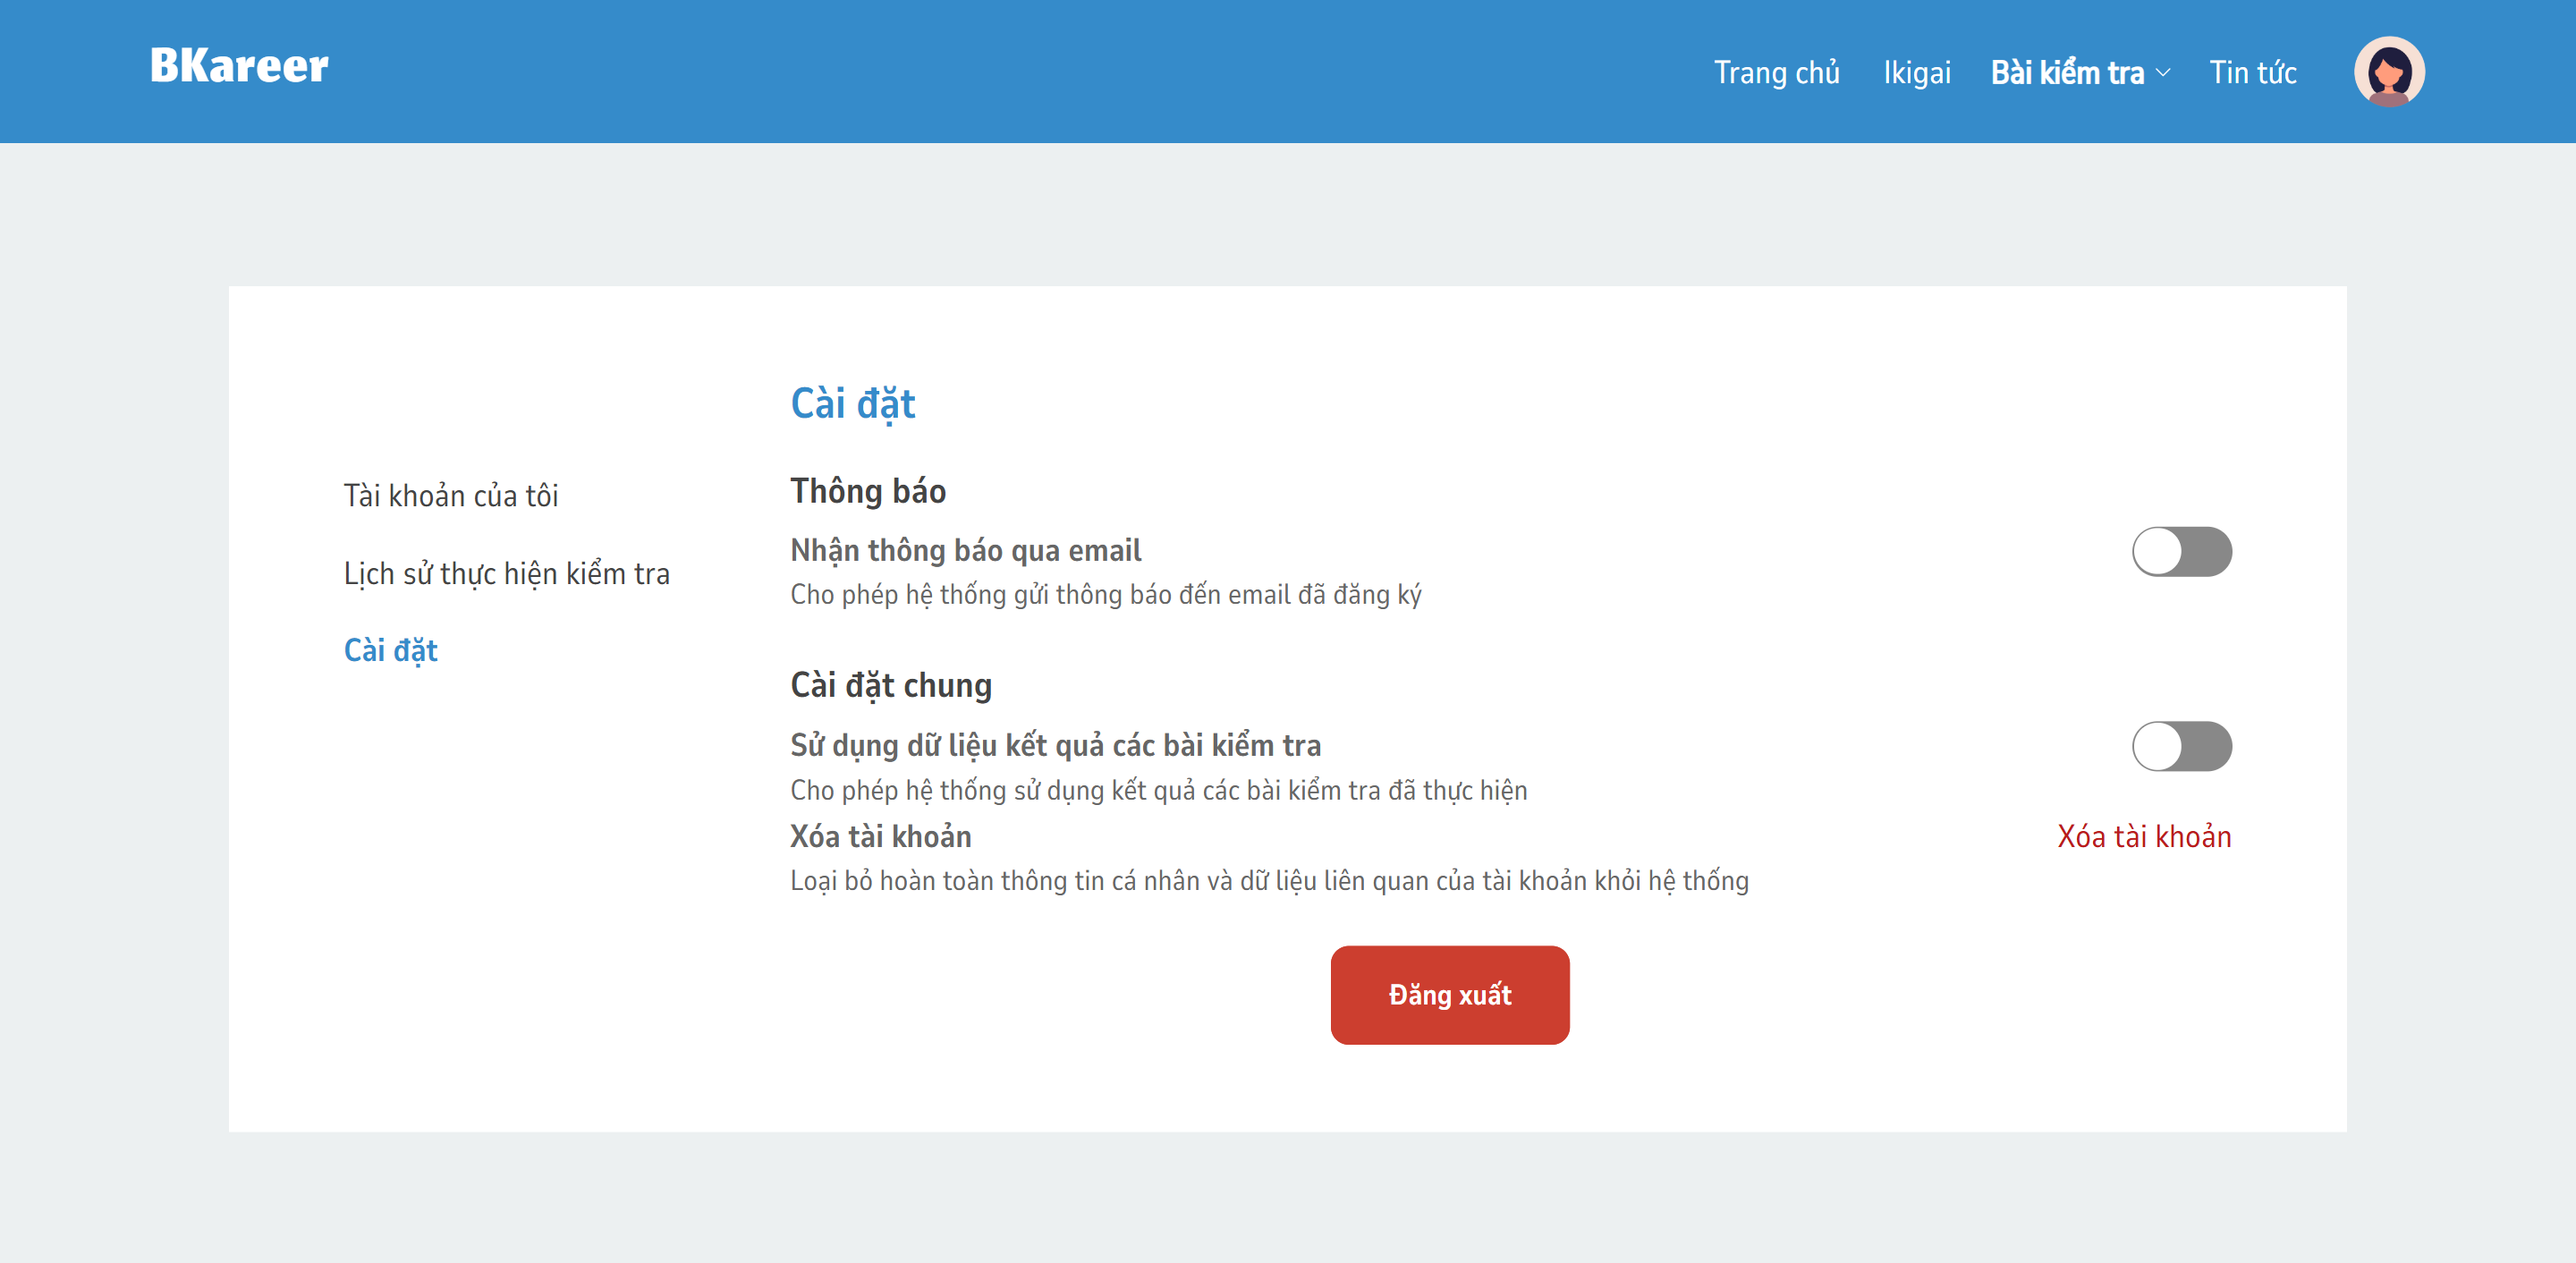
\includegraphics[width=0.8\linewidth]{images/chap5/profile-Setting.png}
    \vspace{0.5cm}
    \caption{Trang cài đặt}
\end{figure}

Các thành phần chính của trang cài đặt:
\begin{itemize}
    \item Tên tab: Tên tab cung cấp thông tin sơ lược về nội dung sẽ được hiển thị trong tab đó.
    \item Thông báo:
        \begin{itemize}
            \item Nhận thông báo qua email: Tùy chỉnh của người dùng về việc cho phép hệ thống gửi thông báo đến email đã đăng ký. 
        \end{itemize}
    \item Cài đặt chung:
        \begin{itemize}
            \item Sử dụng dữ liệu kết quả các bài kiểm tra: Tùy chỉnh của người dùng về việc cho phép hệ thống sử dụng kết quả các bài kiểm tra đã thực hiện để phục vụ cho việc cải tiến và hoàn thiện hệ thống.
            \item Xóa tài khoản: Cho phép người dùng loại bỏ hoàn toàn thông tin cá nhân và dữ liệu liên quan của tài khoản khỏi hệ thống khi không còn sử dụng hệ thống để ngăn chặn thông tin cá nhân bị rò rỉ hoặc sử dụng trái phép.
        \end{itemize}
    \item Nút:
        \begin{itemize}
            \item Nút ``Đăng xuất": Khi người dùng nhấn vào nút này, hệ thống sẽ xác nhận và kết thúc phiên làm việc hiện tại, đưa người dùng trở lại trang đăng nhập.
        \end{itemize}
\end{itemize}


%%%%%%%%%% Ikigai Screen %%%%%%%%%%
\subsection{Trang giới thiệu về Ikigai}
Trang giới thiệu về Ikigai là một không gian trực tuyến cung cấp thông tin chi tiết, dễ hiểu về khái niệm Ikigai – một triết lý sống của người Nhật, xoay quanh việc tìm kiếm mục đích sống. Trang này thường có mục tiêu giúp người đọc hiểu rõ Ikigai là gì, mô tả 4 yếu tố chính tạo nên Ikigai, và hướng dẫn người dùng tìm kiếm Ikigai.

Mục đích của trang giới thiệu về Ikigai:
\begin{itemize}
    \item Giải thích và phổ biến khái niệm Ikigai: Đưa ra định nghĩa chi tiết, dễ hiểu về Ikigai, giúp người đọc hình dung rõ ràng về khái niệm này.
    \item Hướng dẫn tìm kiếm Ikigai: Đưa ra một lộ trình cụ thể, từng bước để giúp người đọc khám phá và theo đuổi Ikigai.
    \item Khuyến khích hành động: Khuyến khích người đọc bắt đầu hành động để tìm kiếm và sống theo Ikigai của mình.
\end{itemize}

\begin{figure}[H]
    \centering
    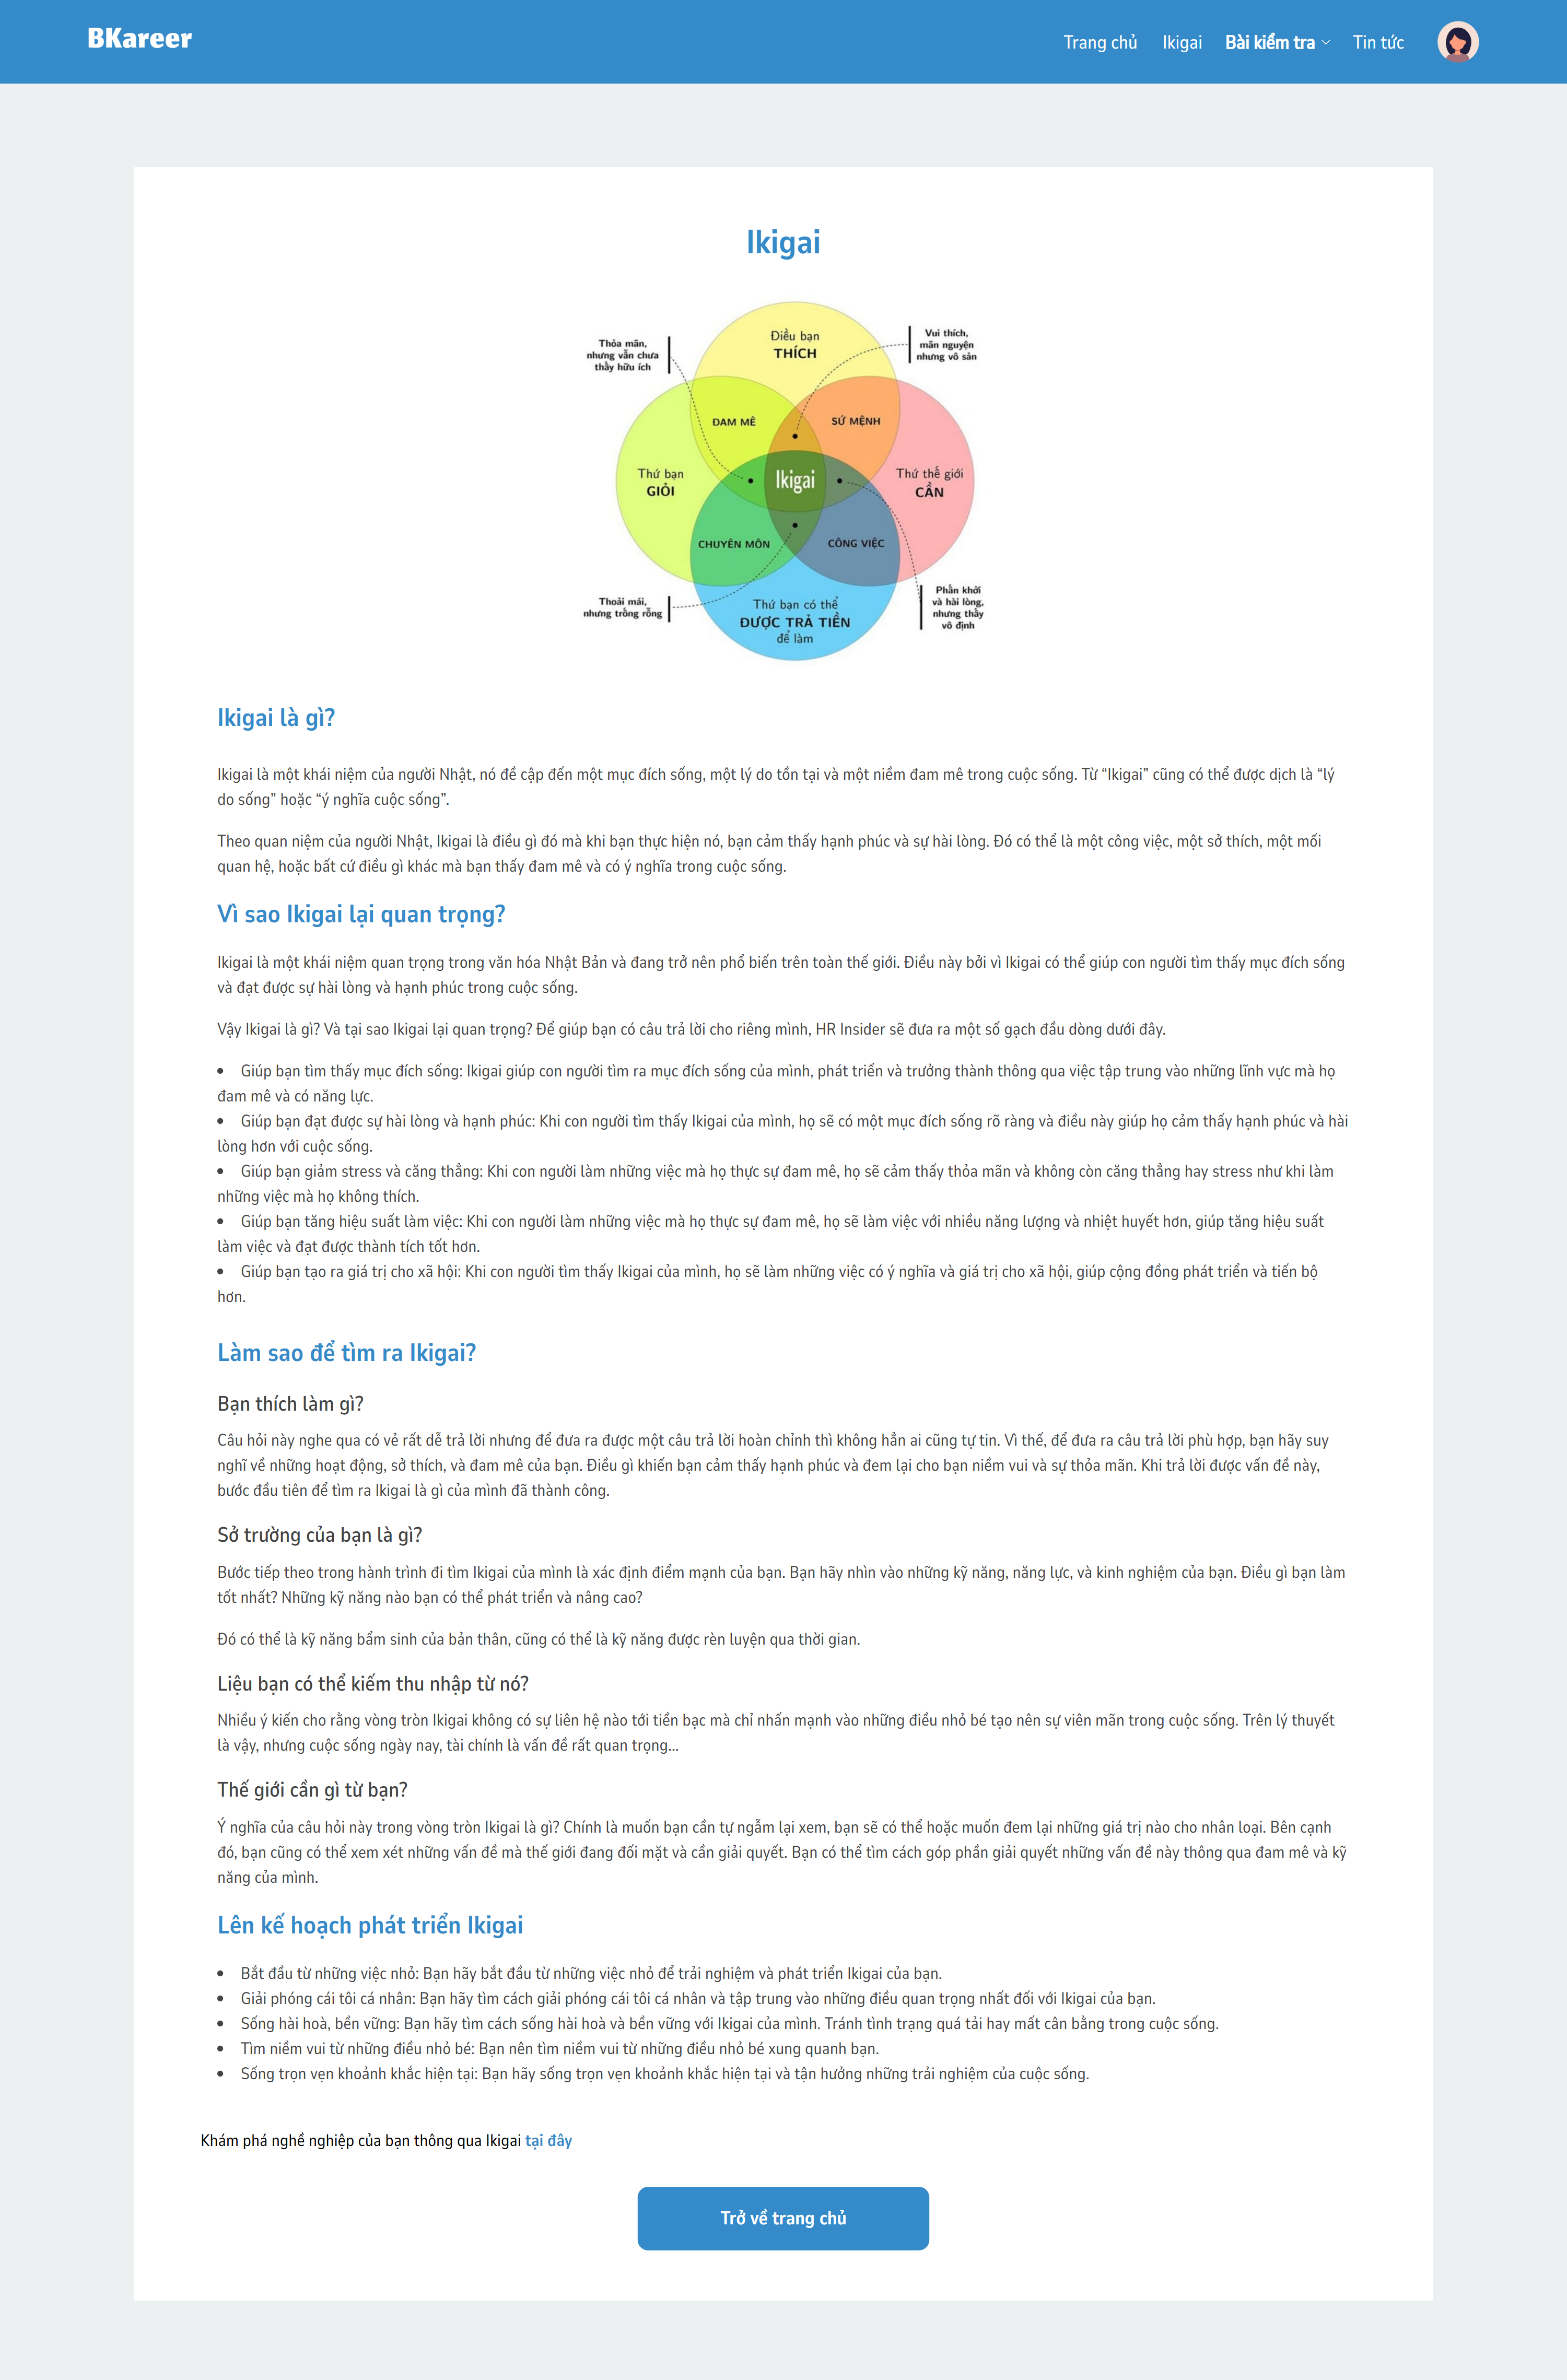
\includegraphics[width=0.8\textwidth]
    {images/chap5/ikigai.png}
    \vspace{0.5cm}
    \caption{Trang giới thiệu về Ikigai}
\end{figure}

Các thành phần chính của trang giới thiệu về Ikigai:
\begin{itemize}
    \item Hình ảnh minh họa: Hình ảnh minh họa cho nội dung của trang giúp người dùng có thể hình dung sơ lược về trang.
    \item Phần giới thiệu: Phần giới thiệu có vai trò cung cấp thông tin cần thiết cho người dùng, giúp người dùng hiểu rõ hơn về mục đích, nội dung và thành phần bài kiểm tra, từ đó có sự chuẩn bị tốt hơn.
    \item Nút:
        \begin{itemize}
            \item Nút ``tại đây": Cho phép người dùng khám phá thêm nghề nghiệp của mình thông qua Ikigai bằng cách thực hiện kiểm tra định hướng ngành nghề. 
            \item Nút ``Trở về trang chủ": Cho phép người dùng quay trở về trang chủ để có thể tìm hiểu thêm những thông tin khác.
        \end{itemize}
\end{itemize}


%%%%%%%%%% News Screen %%%%%%%%%%
\subsection{Trang tin tức}
Trang tin tức là một nền tảng trực tuyến cung cấp thông tin cập nhật , chuyên sâu về các hoạt động nghiên cứu, công bố khoa học, sự kiện học thuật, và các vấn đề liên quan đến lĩnh vực giáo dục đại học trong và ngoài nước. Đây là một kênh thông tin nhanh chóng, tiện lợi và phổ biến, giúp người dùng nắm bắt được những tin tức mới nhất một cách dễ dàng.

Mục đích của trang tin tức:
\begin{itemize}
    \item Cung cấp thông tin: Cập nhật những nghiên cứu mới nhất, công bố khoa học, sự kiện học thuật đến cộng đồng học thuật,...
    \item Thông tin về các cơ sở giáo dục: Giới thiệu về các trường đại học, viện nghiên cứu, các chương trình đào tạo, các cơ hội học bổng.
    \item Phổ biến hóa kiến thức: Đưa những kiến thức chuyên sâu một cách dễ hiểu, giúp công chúng tiếp cận được với những thành tựu khoa học mới nhất.
\end{itemize}

\begin{figure}[H]
    \centering
    \includegraphics[width=0.8\textwidth]
    {images/chap5/news.png}
    \vspace{0.5cm}
    \caption{Trang tin tức}
\end{figure}

Các thành phần chính của trang tin tức:
\begin{itemize}
    \item Các khối tin tức: Mỗi khối thể hiện 1 tin tức, bao gồm hình ảnh minh họa cho nội dung tin tức, tiêu đề, và một phần ngắn tin tức trích từ tin tức đầy đủ, thời gian tin tức xuất hiện.
    \item Nút:
        \begin{itemize}
            \item Phân trang: Dùng để chia một lượng lớn dữ liệu thành các trang nhỏ hơn, dễ quản lý và hiển thị hơn. Điều này giúp người dùng dễ dàng tìm kiếm và xem thông tin mà không bị quá tải.
        \end{itemize}
\end{itemize}


%%%%%%%%%% Major Test Screen %%%%%%%%%%
\subsection{Trang kiểm tra định hướng ngành nghề}
Trang kiểm tra định hướng ngành nghề là bài kiểm tra trực tuyến được thiết kế để giúp người dùng khám phá và đánh giá sự phù hợp của mình với các ngành nghề phù hợp khác nhau. Trang này sẽ bao gồm phần giới thiệu và các thành phần của bài kiểm tra.

Mục đích của trang kiểm tra định hướng ngành nghề:
\begin{itemize}
    \item Hiểu rõ bản thân: Nhận biết rõ hơn về điểm mạnh, điểm yếu, sở thích, giá trị quan và tính cách của mình.
    \item Khám phá các lựa chọn nghề nghiệp: Mở rộng hiểu biết về các ngành nghề khác nhau và những yêu cầu mà mỗi ngành nghề đòi hỏi.
    \item So sánh và đánh giá: So sánh các ngành nghề khác nhau để tìm ra những ngành phù hợp nhất với bản thân.
    \item Đưa ra quyết định: Cung cấp thông tin và cơ sở để người dùng đưa ra quyết định về việc lựa chọn ngành học hoặc nghề nghiệp trong tương lai.
\end{itemize}

\begin{figure}[H]
    \centering
    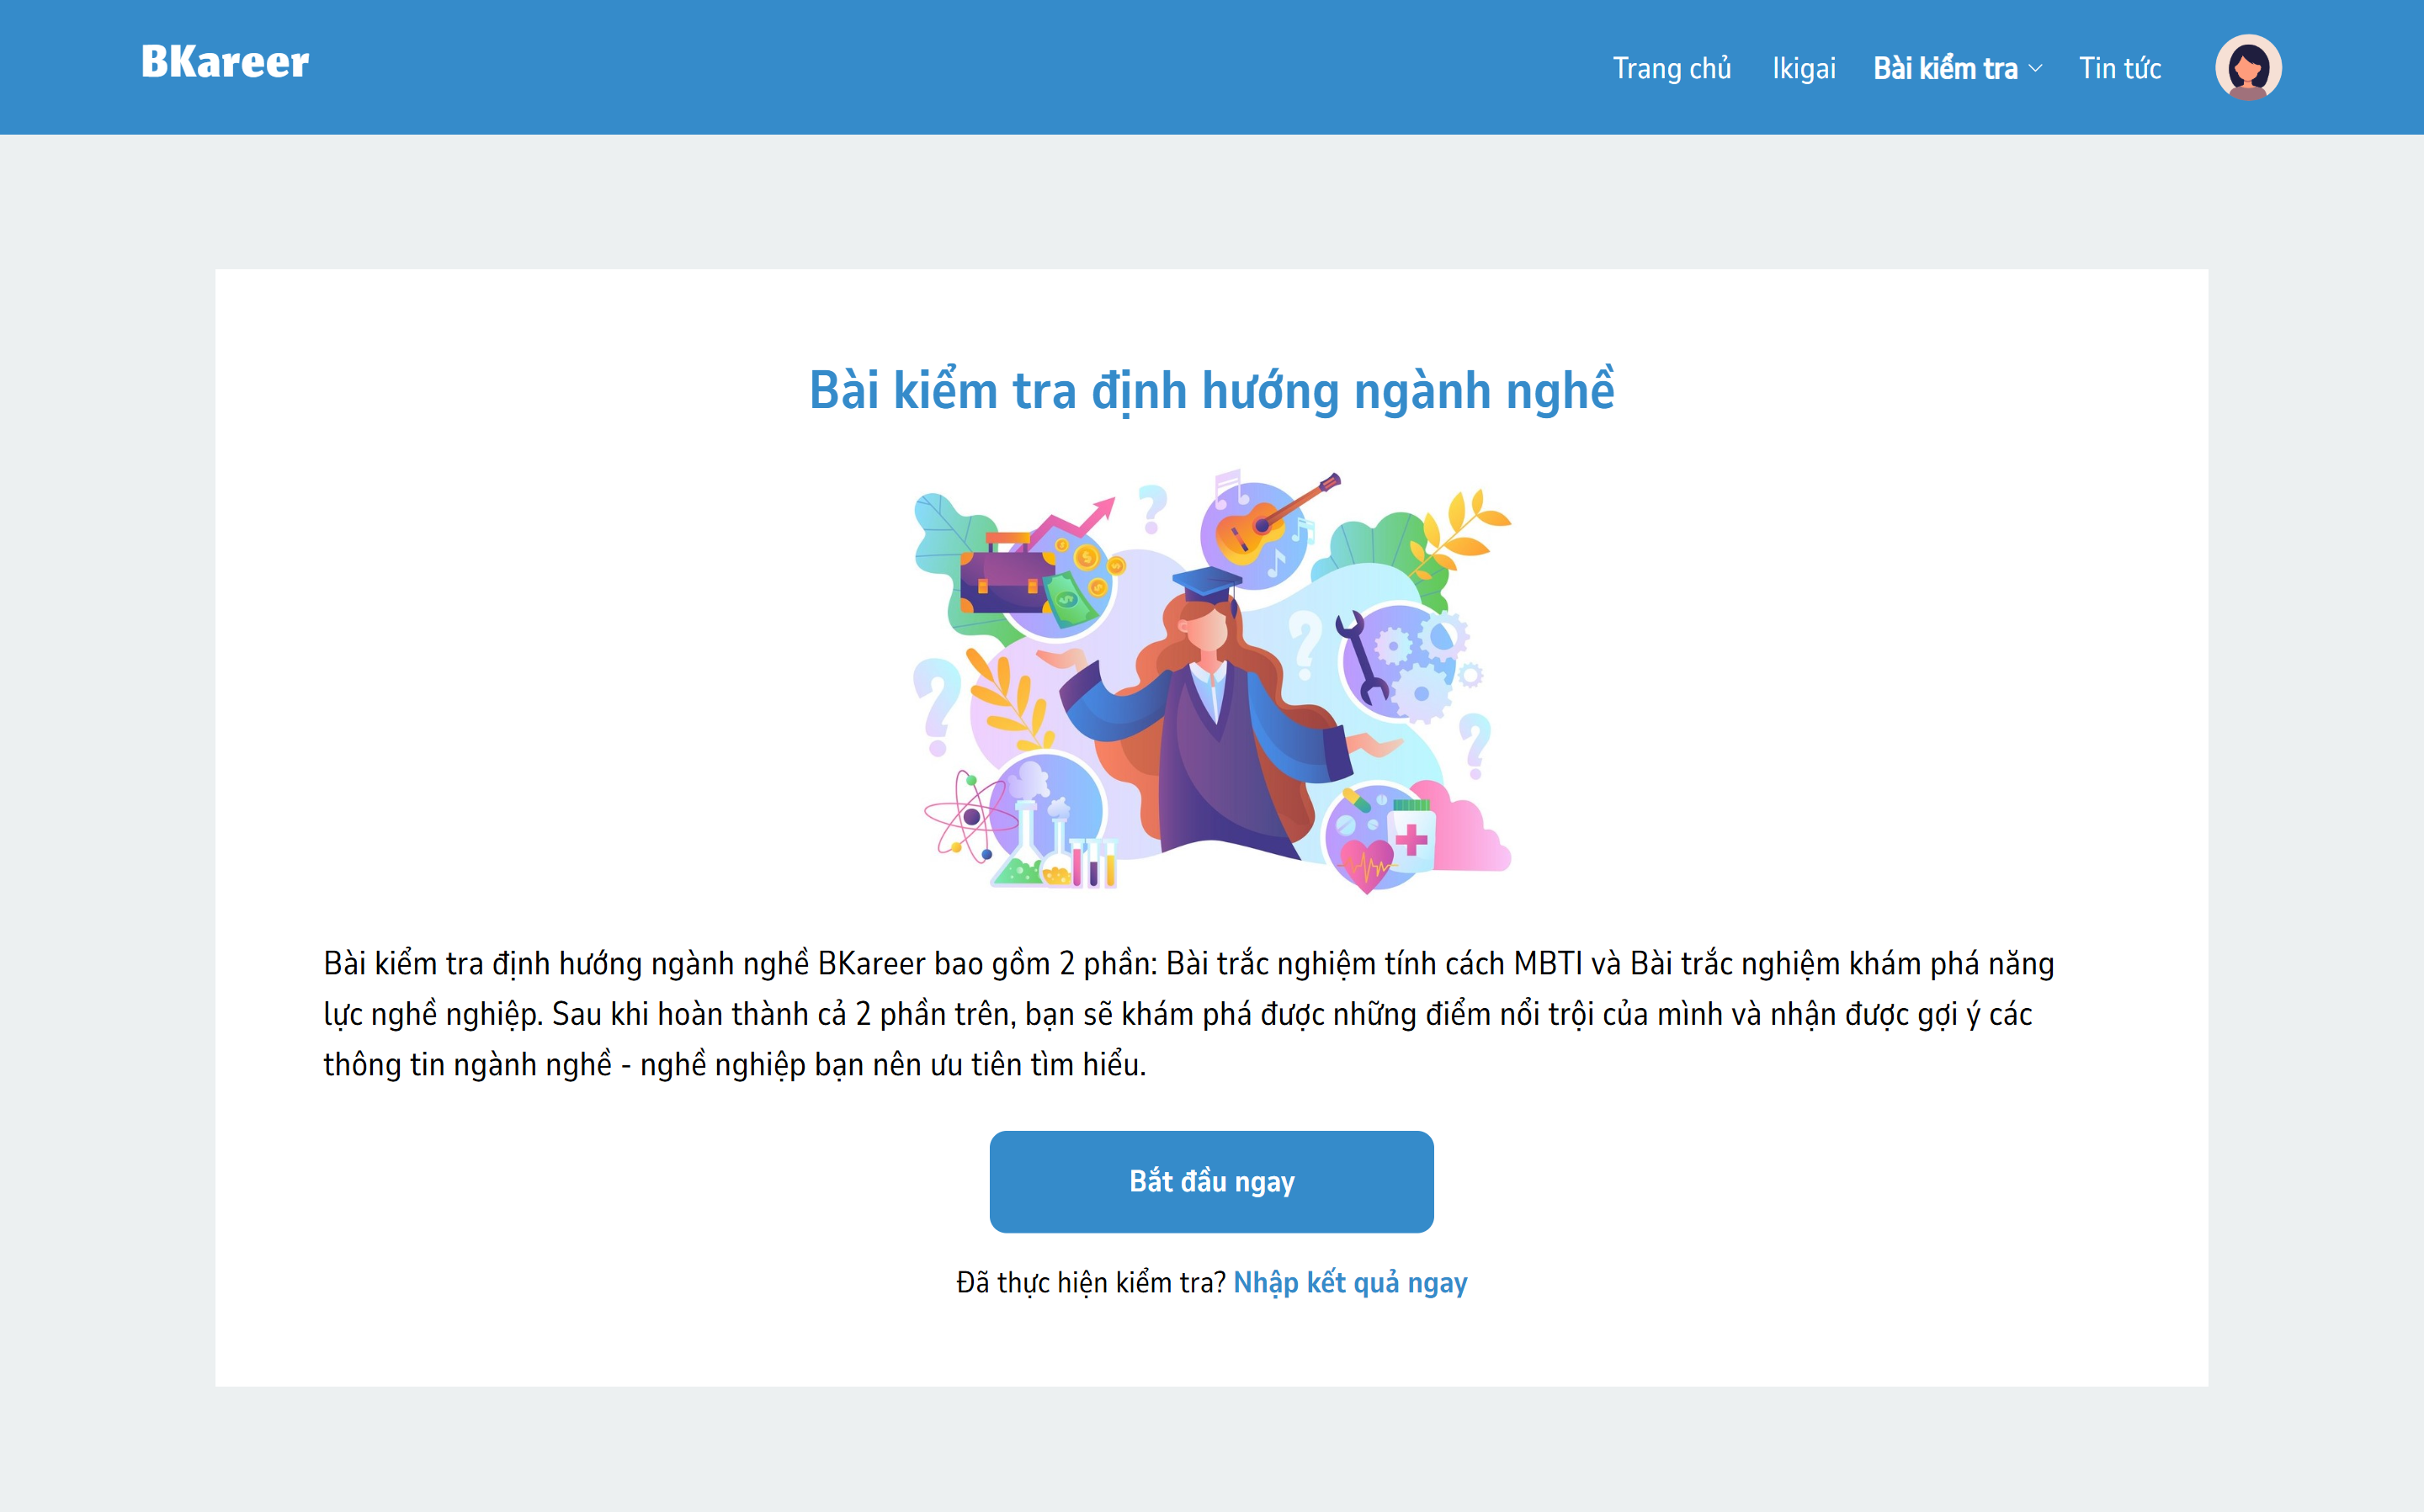
\includegraphics[width=0.8\linewidth]{images/chap5/majorTest.png}
    \vspace{0.5cm}
    \caption{Trang kiểm tra định hướng ngành nghề}
\end{figure}

Các thành phần chính của trang kiểm tra định hướng ngành nghề:
\begin{itemize}
    \item Hình ảnh minh họa: Hình ảnh minh họa cho nội dung của trang giúp người dùng có thể hình dung sơ lược về trang.
    \item Phần giới thiệu: Phần giới thiệu có vai trò cung cấp thông tin cần thiết cho người dùng, giúp người dùng hiểu rõ hơn về mục đích, nội dung và thành phần bài kiểm tra, từ đó có sự chuẩn bị tốt hơn.
    \item Nút:
        \begin{itemize}
            \item Nút ``Bắt đầu ngay": Cho phép người dùng bắt đầu thực hiện bài kiểm tra ngay lập tức.
            \item Nút ``Nhập kết quả ngay": Cho phép người dùng bỏ qua một phần hoặc toàn bộ quá trình kiểm tra nếu người dùng đã từng thực hiện qua các bài kiểm tra từ những nguồn khác, giúp tiết kiệm thời gian cho người dùng.
        \end{itemize}
\end{itemize}


%%%%%%%%%% Major Result %%%%%%%%%%
\subsection{Trang kết quả kiểm tra định hướng ngành nghề}
Trang kết quả kiểm tra định hướng ngành nghề là giao diện hiển thị kết quả 2 bài kiểm tra: trắc nghiệm tính cách MBTI và trắc nghiệm khám phá năng lực nghề nghiệp đi kèm thông tin phân tích kết quả gợi ý ngành nghề phù hợp dưới dạng slide (3 kết quả phù hợp nhất) và dạng bảng (toàn bộ kết quả chi tiết đánh giá mức độ phù hợp cho từng ngành nghề). Đây là phần quan trọng nhất, cung cấp những thông tin giá trị giúp người dùng hiểu rõ hơn về bản thân và định hướng nghề nghiệp tương lai.

Mục đích của trang kết quả kiểm tra định hướng ngành nghề:
\begin{itemize}
    \item Cung cấp kết quả phân tích chi tiết: Dựa trên kết quả phân tích, hệ thống sẽ gợi ý những ngành nghề, lĩnh vực có khả năng phù hợp với tính cách, sở thích và năng lực của người dùng.
    \item Đánh giá sự phù hợp với ngành nghề hiện tại: Nếu người dùng đã có công việc, kết quả kiểm tra sẽ giúp họ đánh giá xem công việc hiện tại có phù hợp với bản thân hay không.
    \item Cung cấp thông tin tham khảo: Cung cấp thông tin chi tiết về các ngành nghề được đề xuất, bao gồm yêu cầu công việc, cơ hội việc làm, mức lương,...
\end{itemize}

\begin{figure}[H]
    \centering
    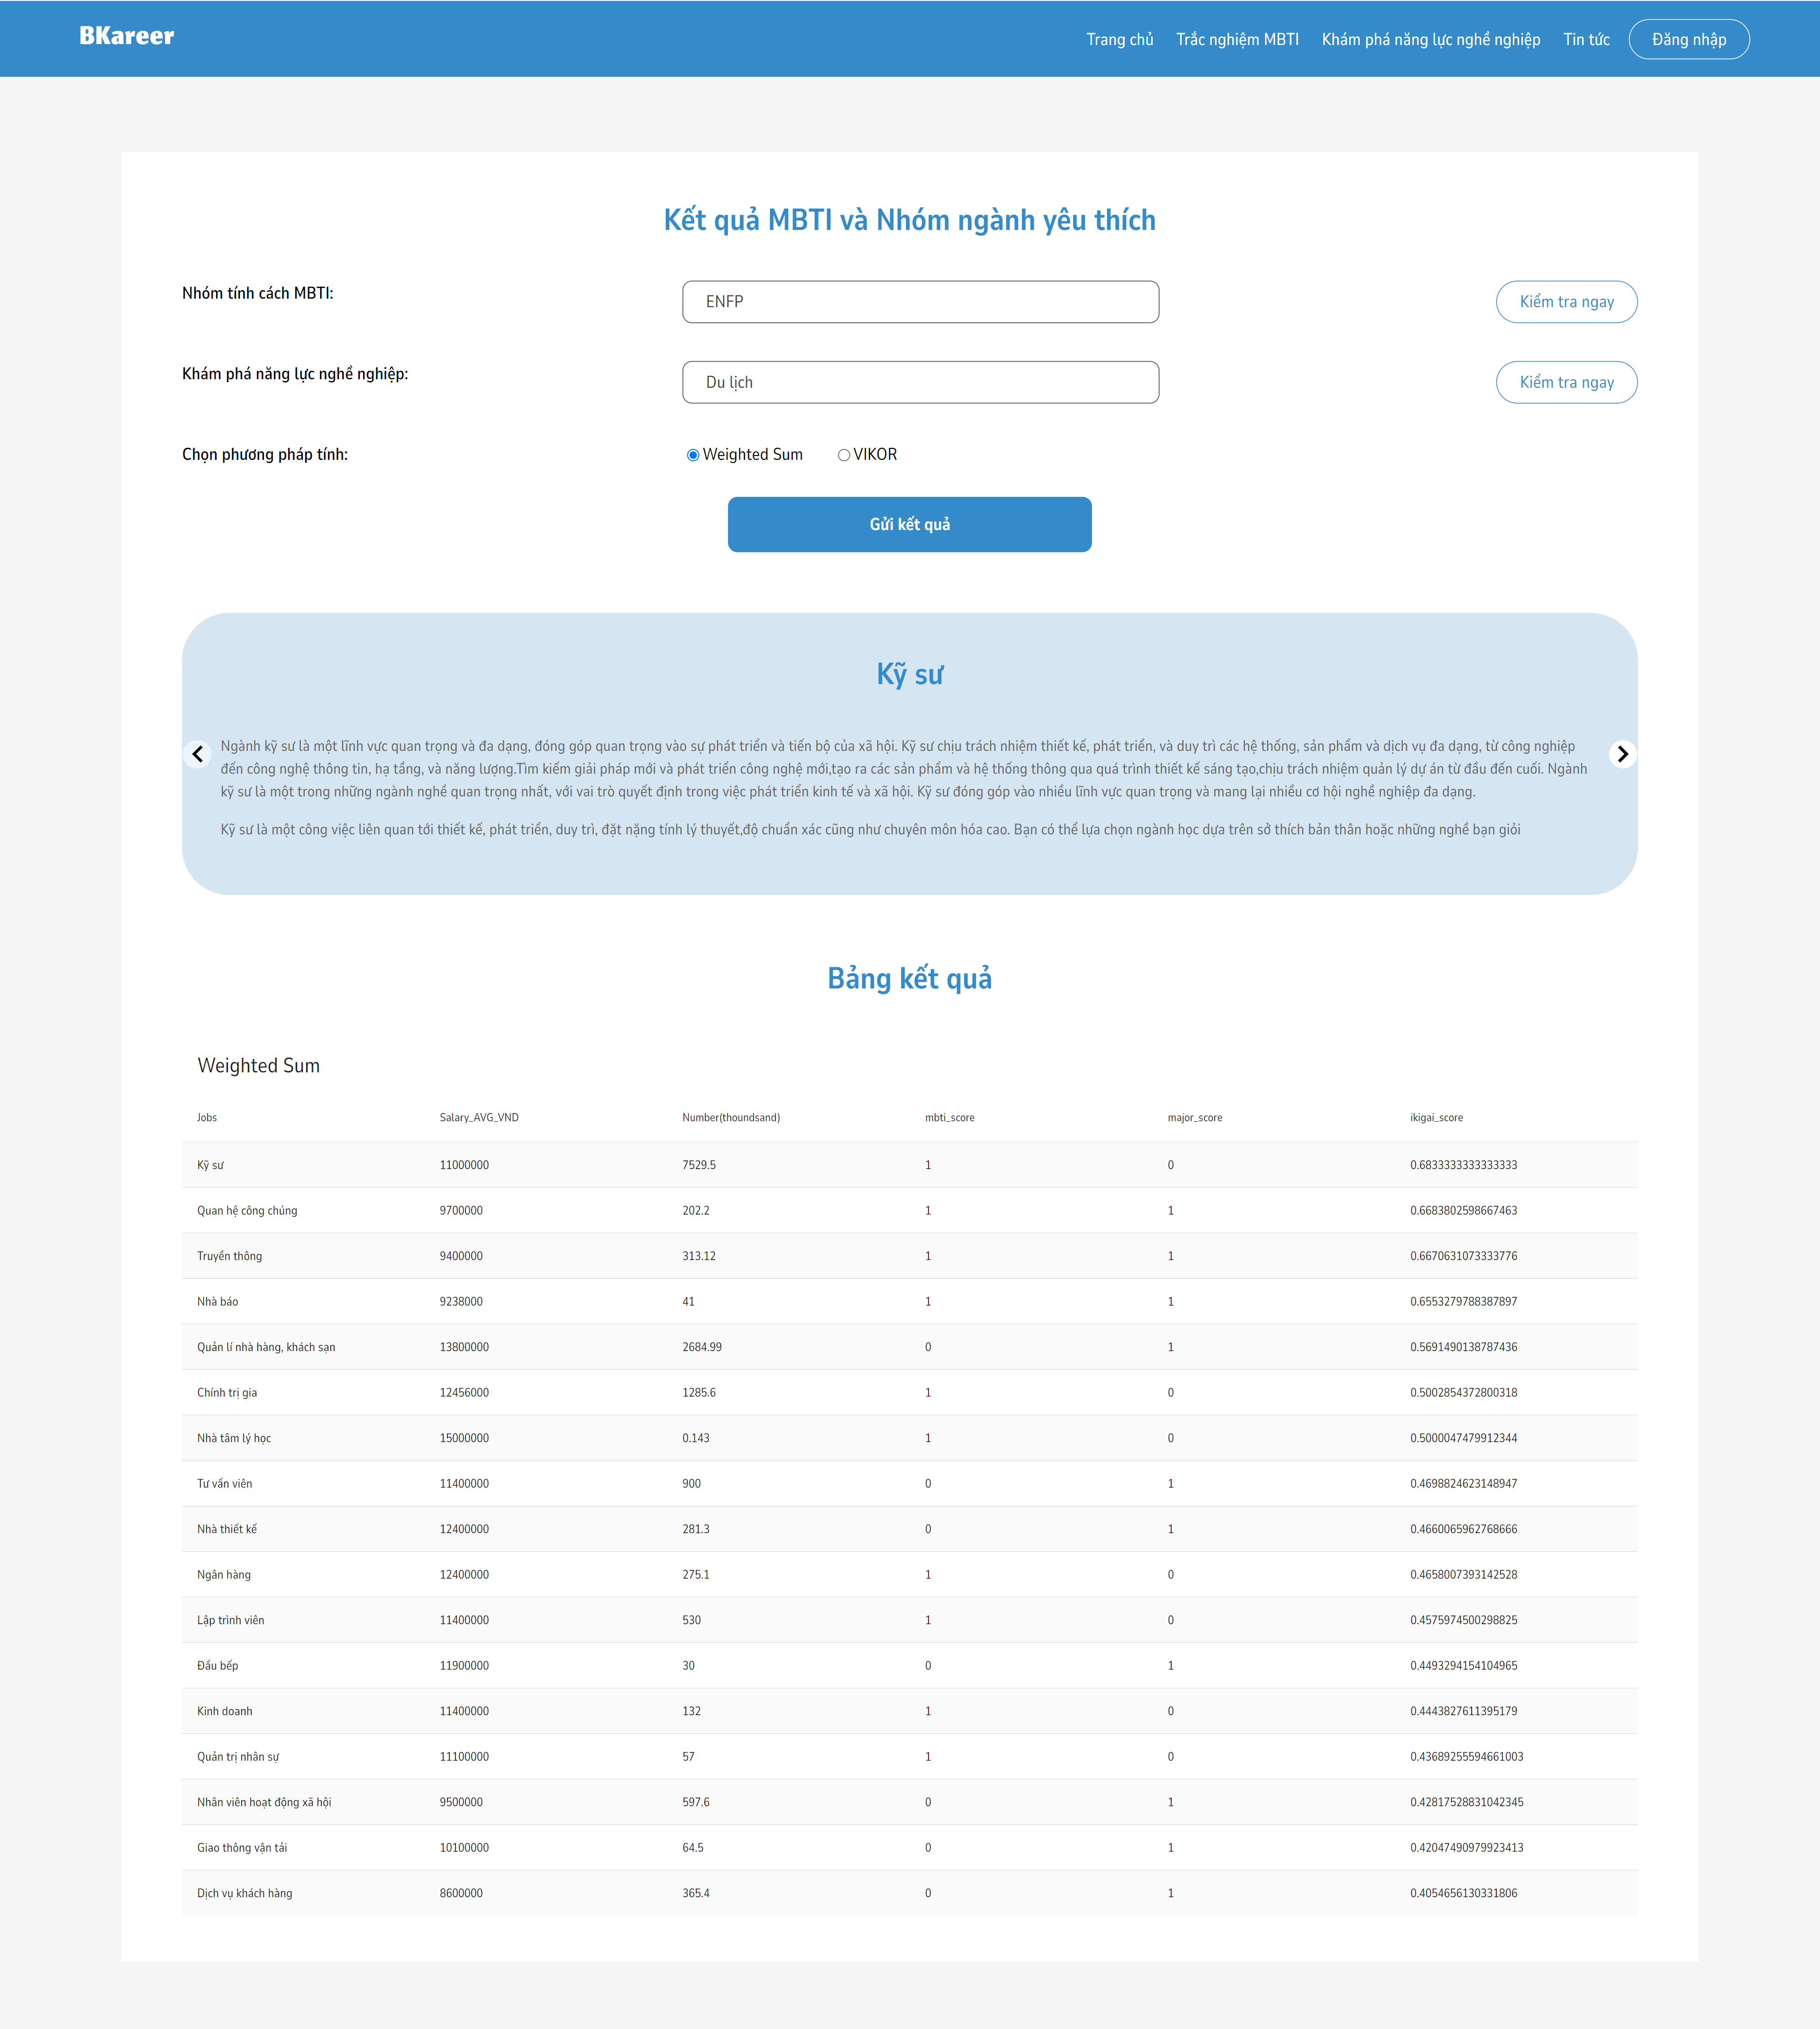
\includegraphics[width=0.8\textwidth]
    {images/chap5/majorResult.png}
    \vspace{0.6cm}
    \caption{Trang kết quả kiểm tra định hướng ngành nghề}
\end{figure}

Các thành phần chính của trang kết quả kiểm tra định hướng ngành nghề:
\begin{itemize}
    \item Nhóm tính cách MBTI: Trình đơn thả xuống bao gồm 16 loại tính cách MBTI, cho phép người dùng lựa chọn loại tính cách của mình.
    \item Khám phá năng lực nghề nghiệp: Trình đơn thả xuống bao gồm 16 loại ngành nghề, cho phép người dùng lựa chọn kết quả của mình.
    \item Chọn phương pháp tính: Cho phép người dùng lựa chọn 1 trong 2 cách tính và phân tích kết quả kiểm tra.
    \item Nút:
        \begin{itemize}
            \item Nút ``Kiểm tra ngay": Cho phép người dùng chuyển đến trang kiểm tra để bắt đầu thực hiện bài kiểm tra ngay lập tức.
            \item Nút ``Gửi kết quả": Cho phép người dùng gửi kết quả đã ghi nhận phía trên để hệ thống tính toán, phân tích và trả về kết quả bên dưới.
        \end{itemize}
    \item Slide: Thể hiện 3 ngành nghề phù hợp nhất dựa trên phân tích theo dữ liệu lấy từ kết quả thực hiện kiểm tra, bao gồm tên ngành nghề và mô tả ngắn gọn về ngành nghề đó.
    \item Bảng kết quả: Thể hiện chi tiết kết quả ghi nhận, phân tích và xếp hạng các ngành nghề phù hợp theo thứ tự giảm dần.
\end{itemize}


%%%%%%%%%% MBTI Detail %%%%%%%%%%
\subsection{Trang giới thiệu trắc nghiệm tính cách MBTI}
Trắc nghiệm tính cách MBTI là một công cụ được thiết kế để giúp người dùng khám phá và hiểu rõ hơn về tính cách của bản thân. MBTI (Myers-Briggs Type Indicator) là một phương pháp phân tích tính cách nổi tiếng, dựa trên lý thuyết của Carl Jung, chia người dùng thành 16 loại tính cách khác nhau dựa trên 4 yếu tố:
\begin{itemize}
    \item Hướng ngoại (E) - Hướng nội (I): Cách con người tương tác với thế giới xung quanh.
    \item Cảm giác (S) - Trực giác (N): Cách con người tiếp nhận thông tin.
    \item Lý trí (T) - Cảm xúc (F): Cách con người đưa ra quyết định.
    \item Quyết đoán (J) - Linh hoạt (P): Cách con người tổ chức cuộc sống.
\end{itemize}

Mục đích của trang giới thiệu trắc nghiệm tính cách MBTI:
\begin{itemize}
    \item Giới thiệu về MBTI: Cung cấp một định nghĩa rõ ràng, dễ hiểu về MBTI là gì, nguồn gốc và cách thức hoạt động của nó. Nêu bật những lợi ích mà MBTI mang lại cho người dùng, như hiểu rõ bản thân hơn, cải thiện các mối quan hệ, lựa chọn nghề nghiệp phù hợp,...
    \item Giới thiệu cấu trúc bài trắc nghiệm: Cung cấp cho người dùng thông tin về số câu hỏi, ước tính thời gian thực hiện và cách thức trả lời các câu hỏi một cách chính xác và trung thực nhất.
\end{itemize}

\begin{figure}[H]
    \centering
    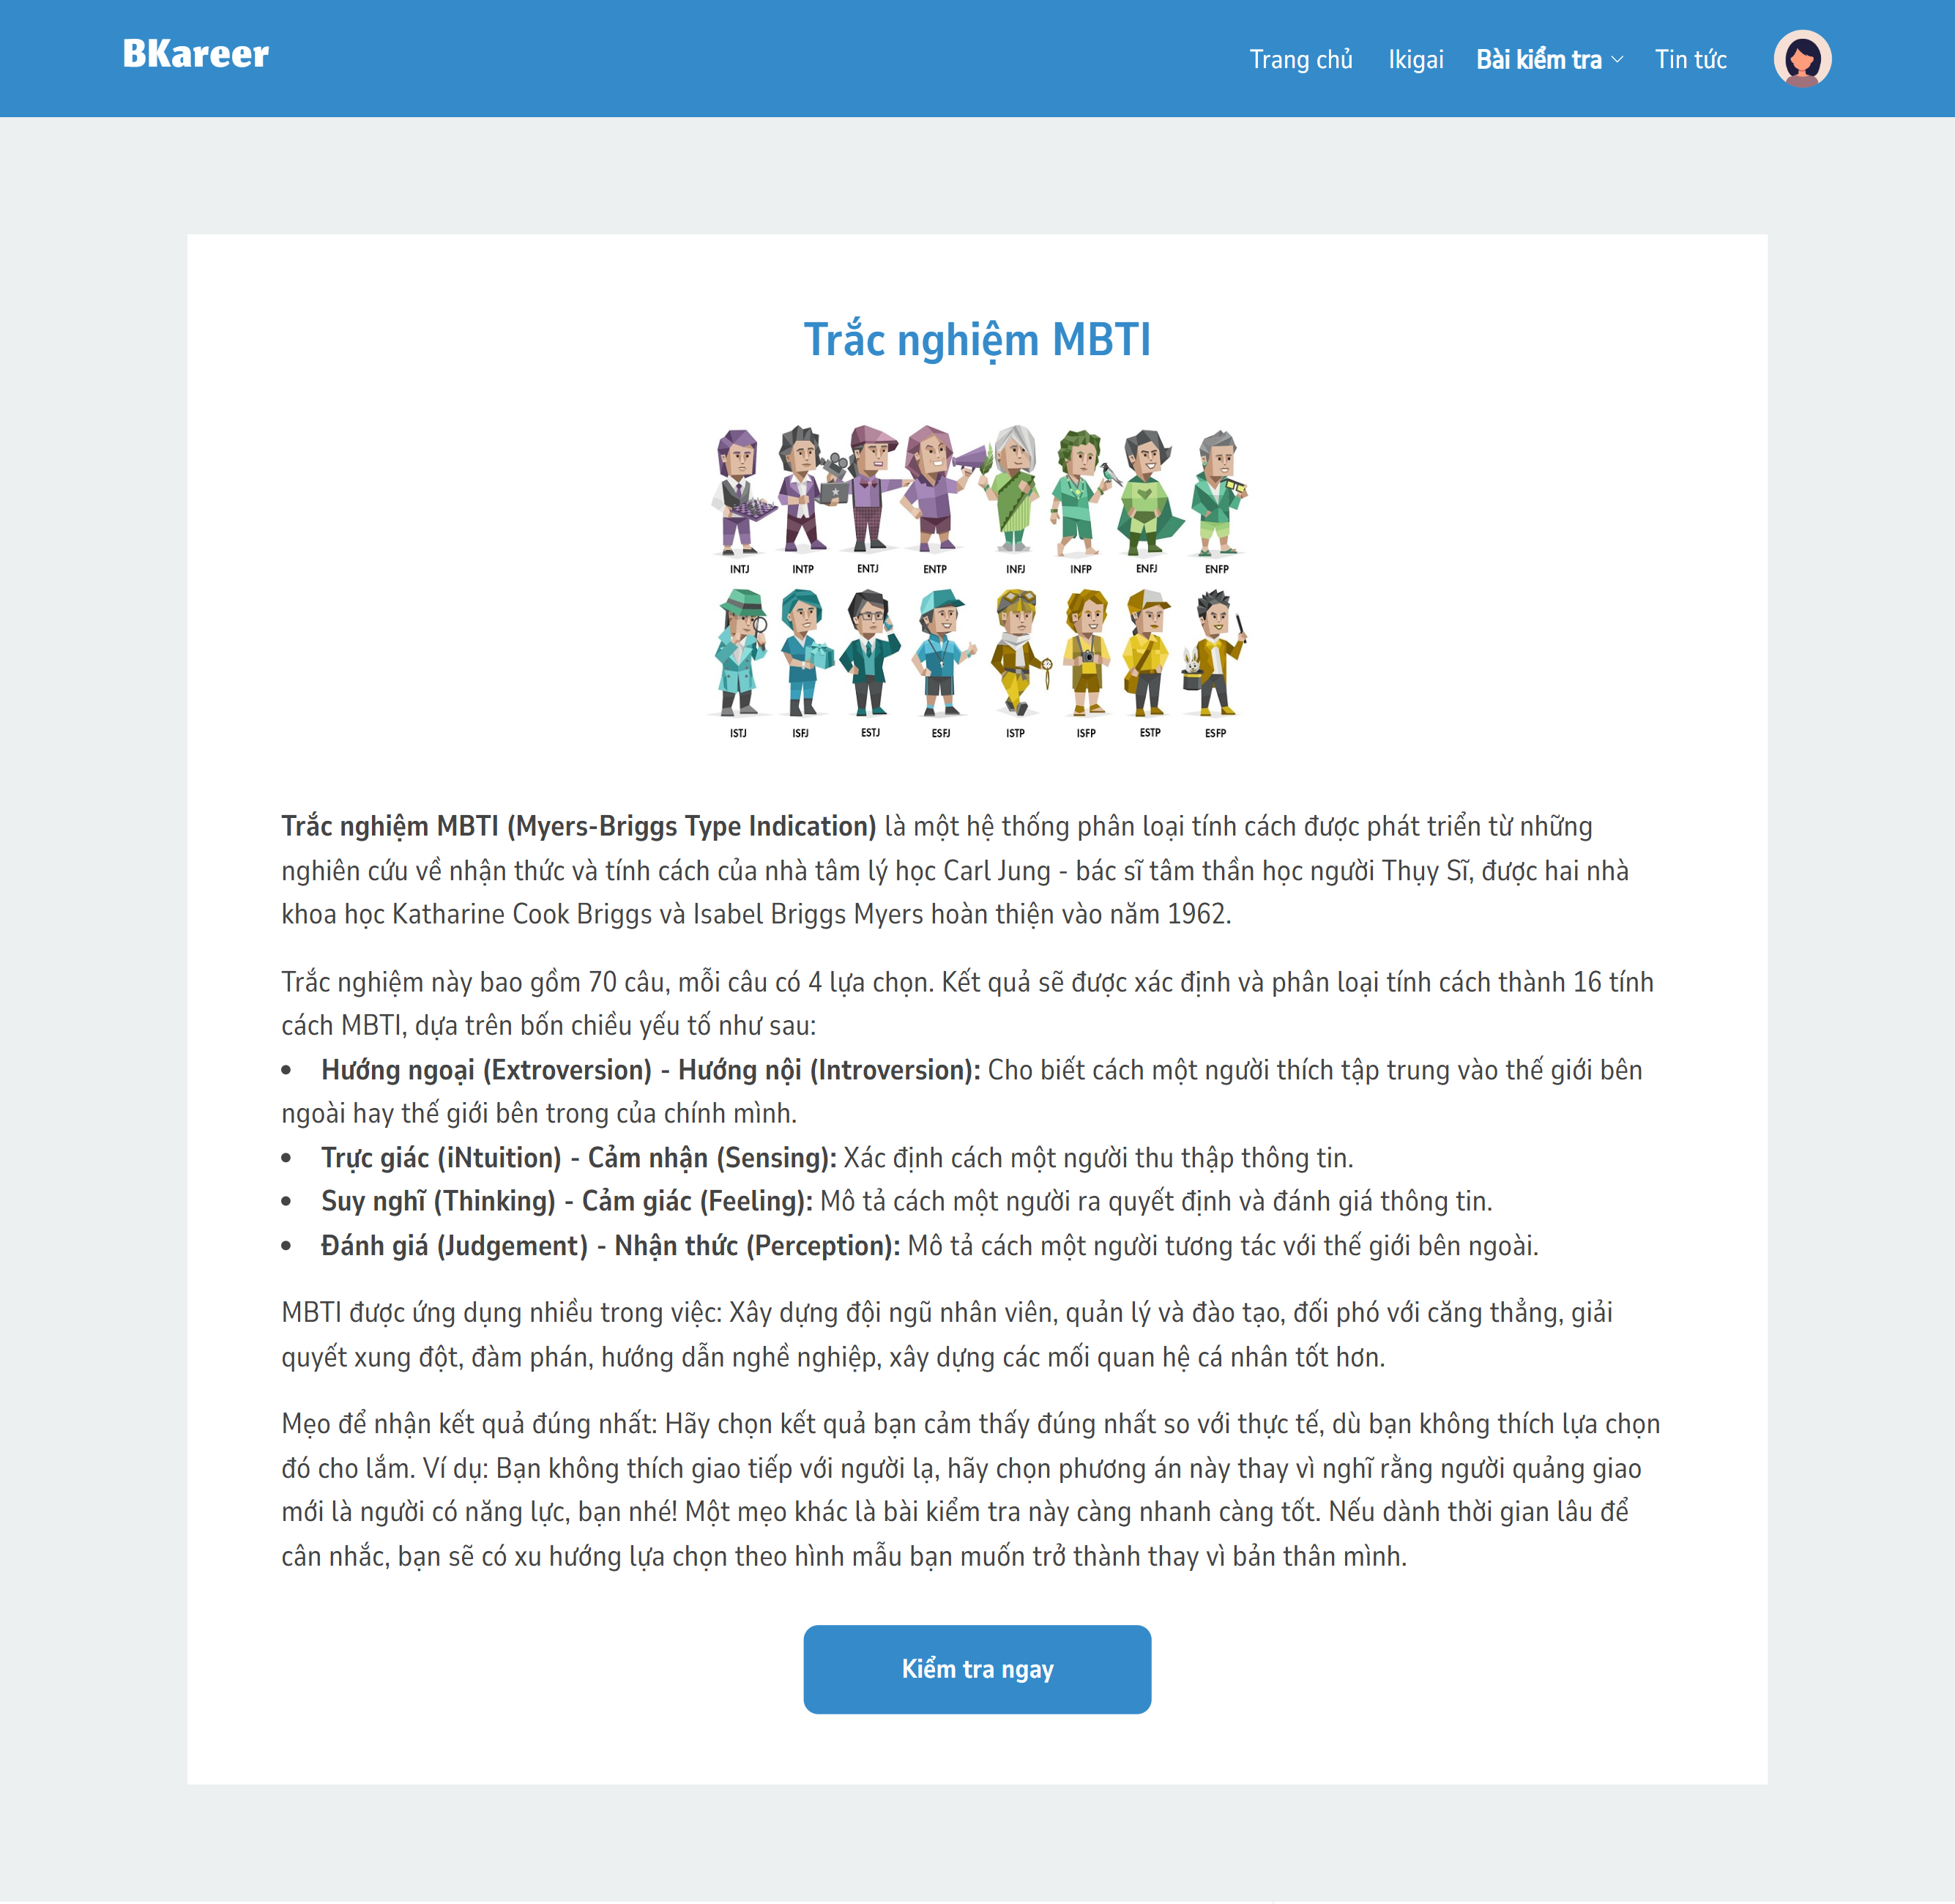
\includegraphics[width=0.8\textwidth]
    {images/chap5/mbtiDetail.png}
    \vspace{0.5cm}
    \caption{Trang giới thiệu trắc nghiệm tính cách MBTI}
\end{figure}

Các thành phần chính của trang giới thiệu trắc nghiệm tính cách MBTI:
\begin{itemize}
    \item Hình ảnh minh họa: Hình ảnh minh họa cho nội dung của trang giúp người dùng có thể hình dung sơ lược về trang.
    \item Phần giới thiệu: Phần giới thiệu có vai trò cung cấp thông tin cần thiết cho người dùng, giúp người dùng hiểu rõ hơn về mục đích, nội dung và thành phần bài kiểm tra, từ đó có sự chuẩn bị tốt hơn.
    \item Nút:
        \begin{itemize}
            \item Nút ``Bắt đầu ngay": Cho phép người dùng bắt đầu thực hiện bài kiểm tra ngay lập tức.
        \end{itemize}
\end{itemize}

%%%%%%%%%% MBTI Test %%%%%%%%%%
\subsection{Trang thực hiện trắc nghiệm tính cách MBTI}
Trang thực hiện trắc nghiệm tính cách MBTI là giao diện trực quan nơi người dùng tương tác trực tiếp với các câu hỏi để đánh giá tính cách của mình. Đây là cầu nối giữa người dùng và kết quả phân tích MBTI. 

Mục đích của trang thực hiện trắc nghiệm tính cách MBTI:
\begin{itemize}
    \item Tạo trải nghiệm người dùng tốt: Giao diện thân thiện, dễ sử dụng, giúp người dùng cảm thấy thoải mái khi thực hiện bài trắc nghiệm.
    \item Thu thập dữ liệu chính xác: Đảm bảo người dùng trả lời các câu hỏi một cách trung thực và đầy đủ.
    \item Cung cấp kết quả chính xác: Sử dụng thuật toán phân tích hiệu quả để đưa ra kết quả chính xác nhất.
\end{itemize}

\begin{figure}[H]
    \centering
    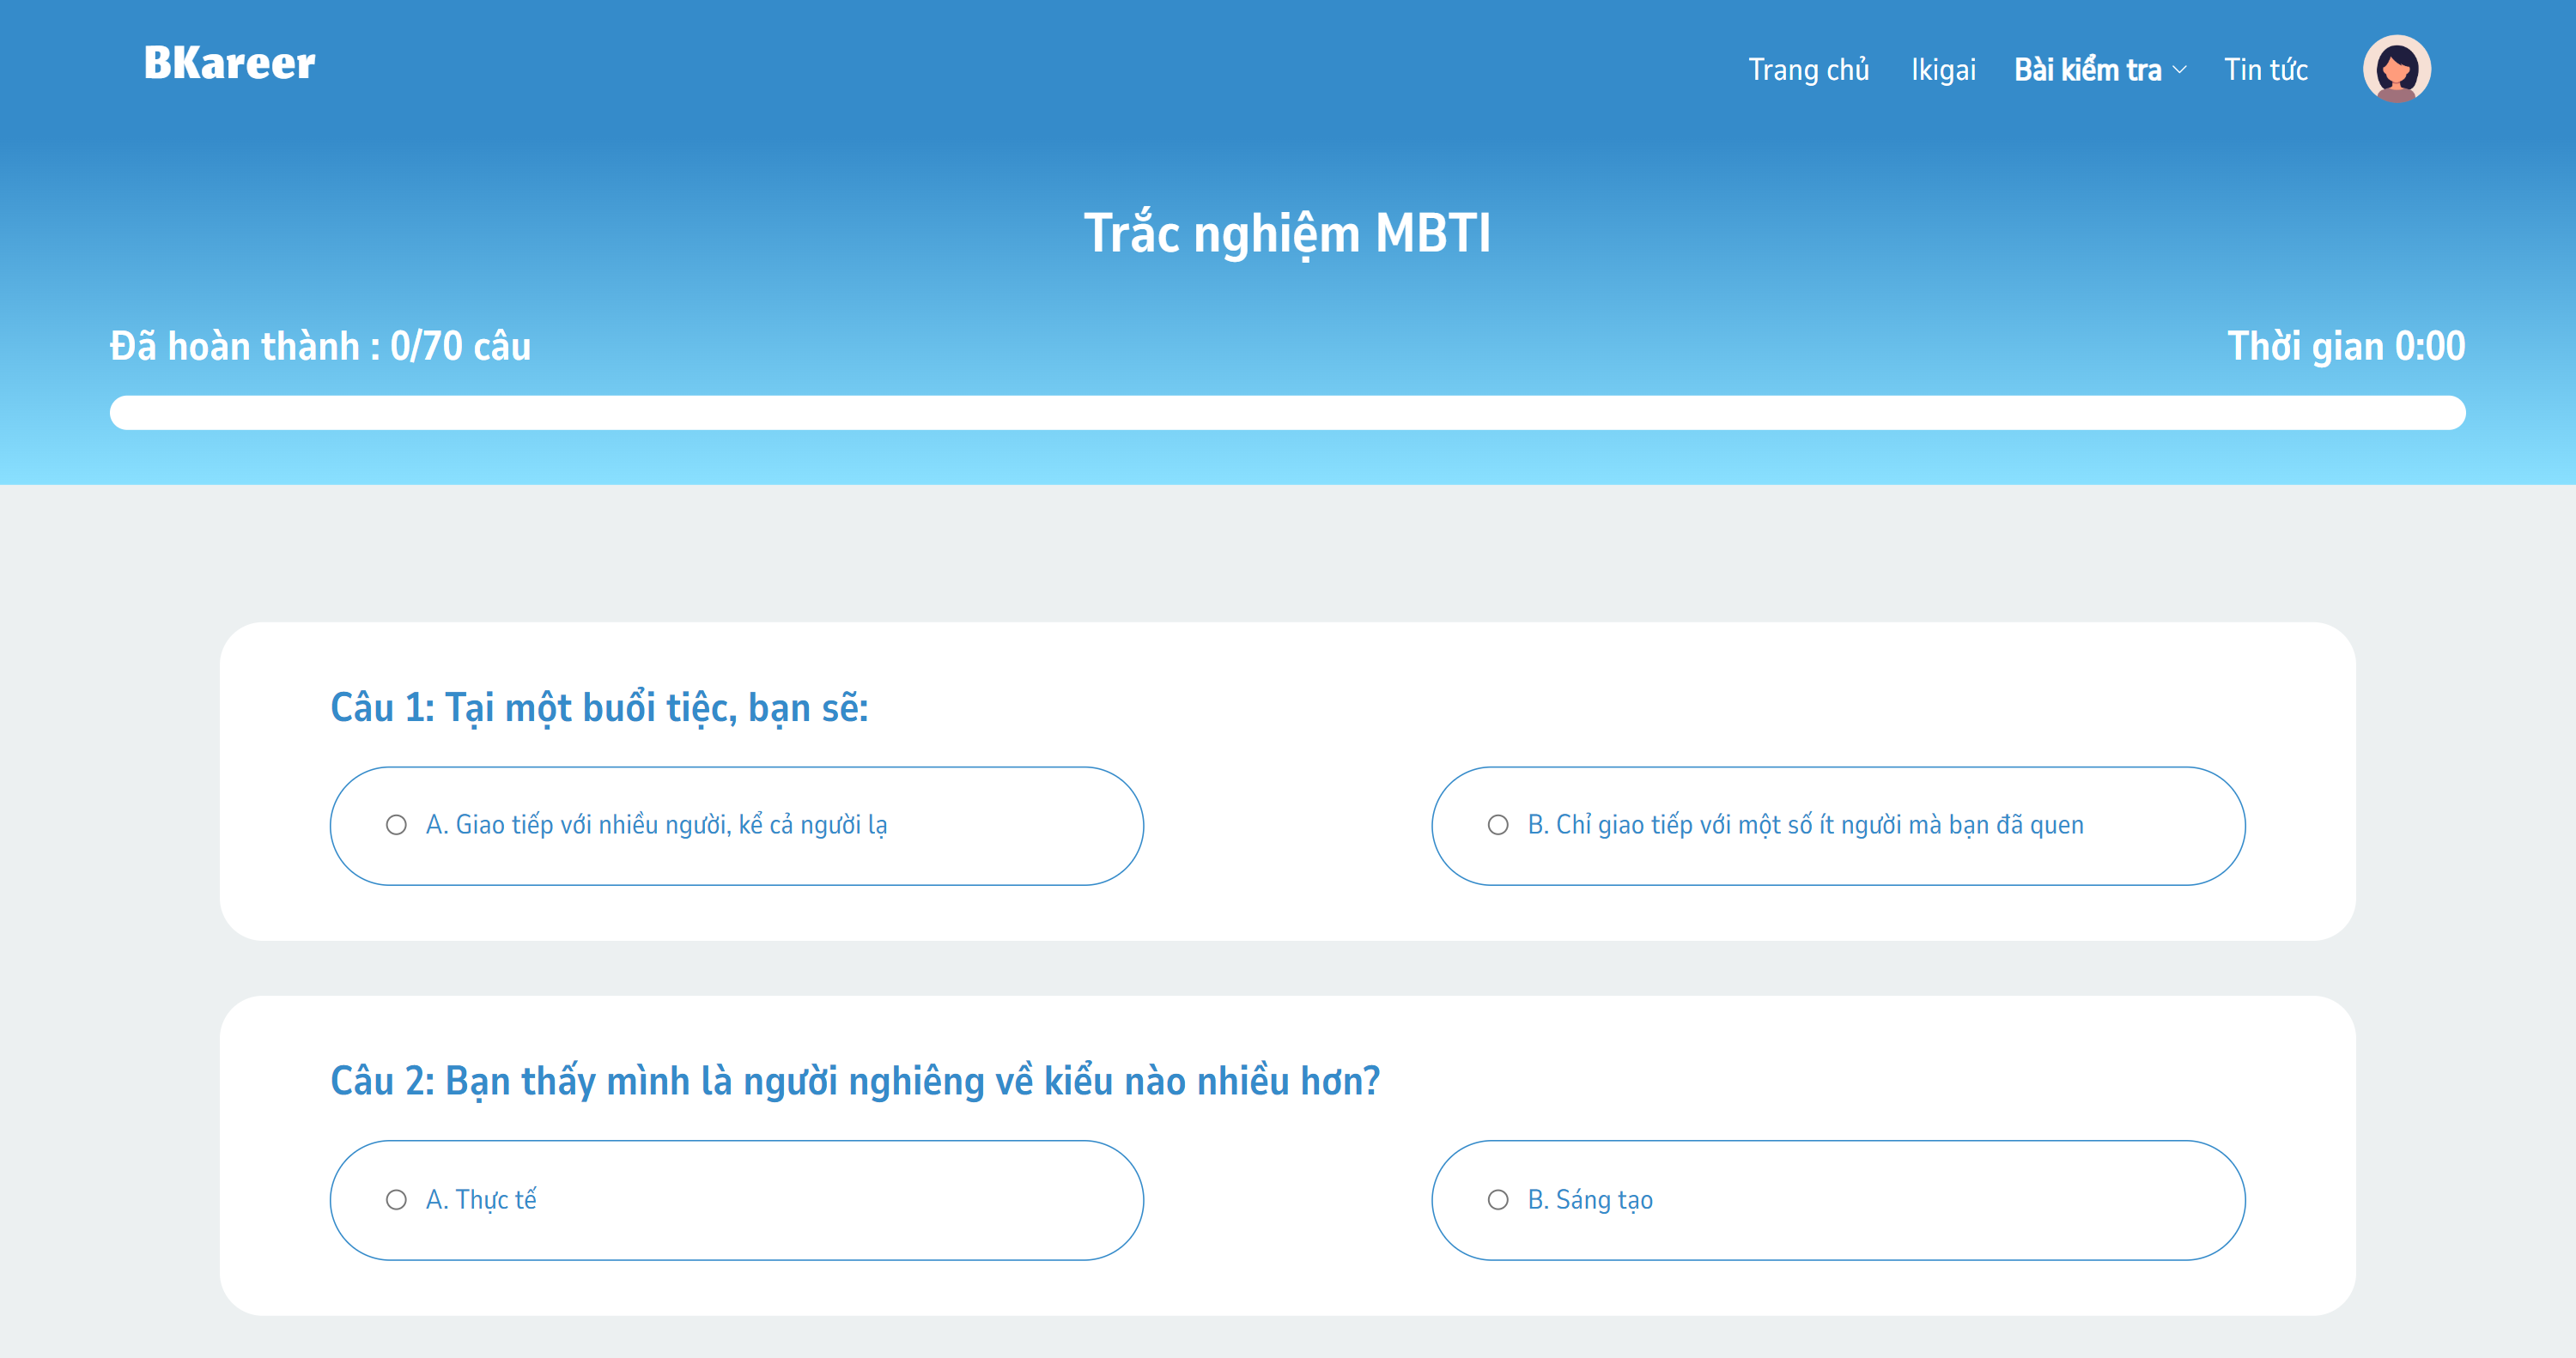
\includegraphics[width=0.8\textwidth]
    {images/chap5/mbti.png}
    \vspace{0.5cm}
    \caption{Trang thực hiện trắc nghiệm tính cách MBTI}
\end{figure}

Các thành phần chính của trang thực hiện trắc nghiệm tính cách MBTI:
\begin{itemize}
    \item Thanh tiến trình: Bao gồm tiến độ hoàn thành bài kiểm tra và đồng hồ đếm thời gian thực hiện bài kiểm tra.
    \item Các khối câu hỏi: Mỗi khối bao gồm 1 câu hỏi và 2 đáp án, cho phép người dùng chọn 1 trong 2 đáp án, và có thể thay đổi sau khi lựa chọn.
    \item Nút:
        \begin{itemize}
            \item Nút ``Quay về nhập kết quả": Cho phép người dùng kết thúc kiểm tra sau khi đã hoàn thành và quay trở về trang nhập kết quả kiểm tra định hướng ngành nghề, hệ thống sẽ tự ghi nhận và điền kết quả vào phần trắc nghiệm MBTI tương ứng.
            \item Nút ``Xem kết quả": Hiển thị giao diện thông báo kết quả cho người dùng.
        \end{itemize}
\end{itemize}


%%%%%%%%%% Career Clustering Detail %%%%%%%%%%
\subsection{Trang giới thiệu trắc nghiệm khám phá năng lực nghề nghiệp}
Trang giới thiệu trắc nghiệm khám phá năng lực nghề nghiệp là một cổng thông tin quan trọng, cung cấp cho người dùng cái nhìn tổng quan về công cụ đánh giá này. Mục tiêu chính của trang là thuyết phục người dùng tham gia thực hiện bài trắc nghiệm để khám phá tiềm năng và định hướng nghề nghiệp phù hợp.

Mục đích của trang giới thiệu trắc nghiệm khám phá năng lực nghề nghiệp:
\begin{itemize}
    \item Giới thiệu về trắc nghiệm khám phá năng lực nghề nghiệp: Cung cấp một định nghĩa rõ ràng, dễ hiểu về bài kiểm tra, nguồn gốc và cách thức hoạt động của nó. Nêu bật những lợi ích mà bài kiểm tra mang lại cho người dùng.
    \item Giới thiệu cấu trúc bài trắc nghiệm: Cung cấp cho người dùng thông tin về số câu hỏi, ước tính thời gian thực hiện và cách thức trả lời các câu hỏi một cách chính xác và trung thực nhất.
\end{itemize}

\begin{figure}[H]
    \centering
    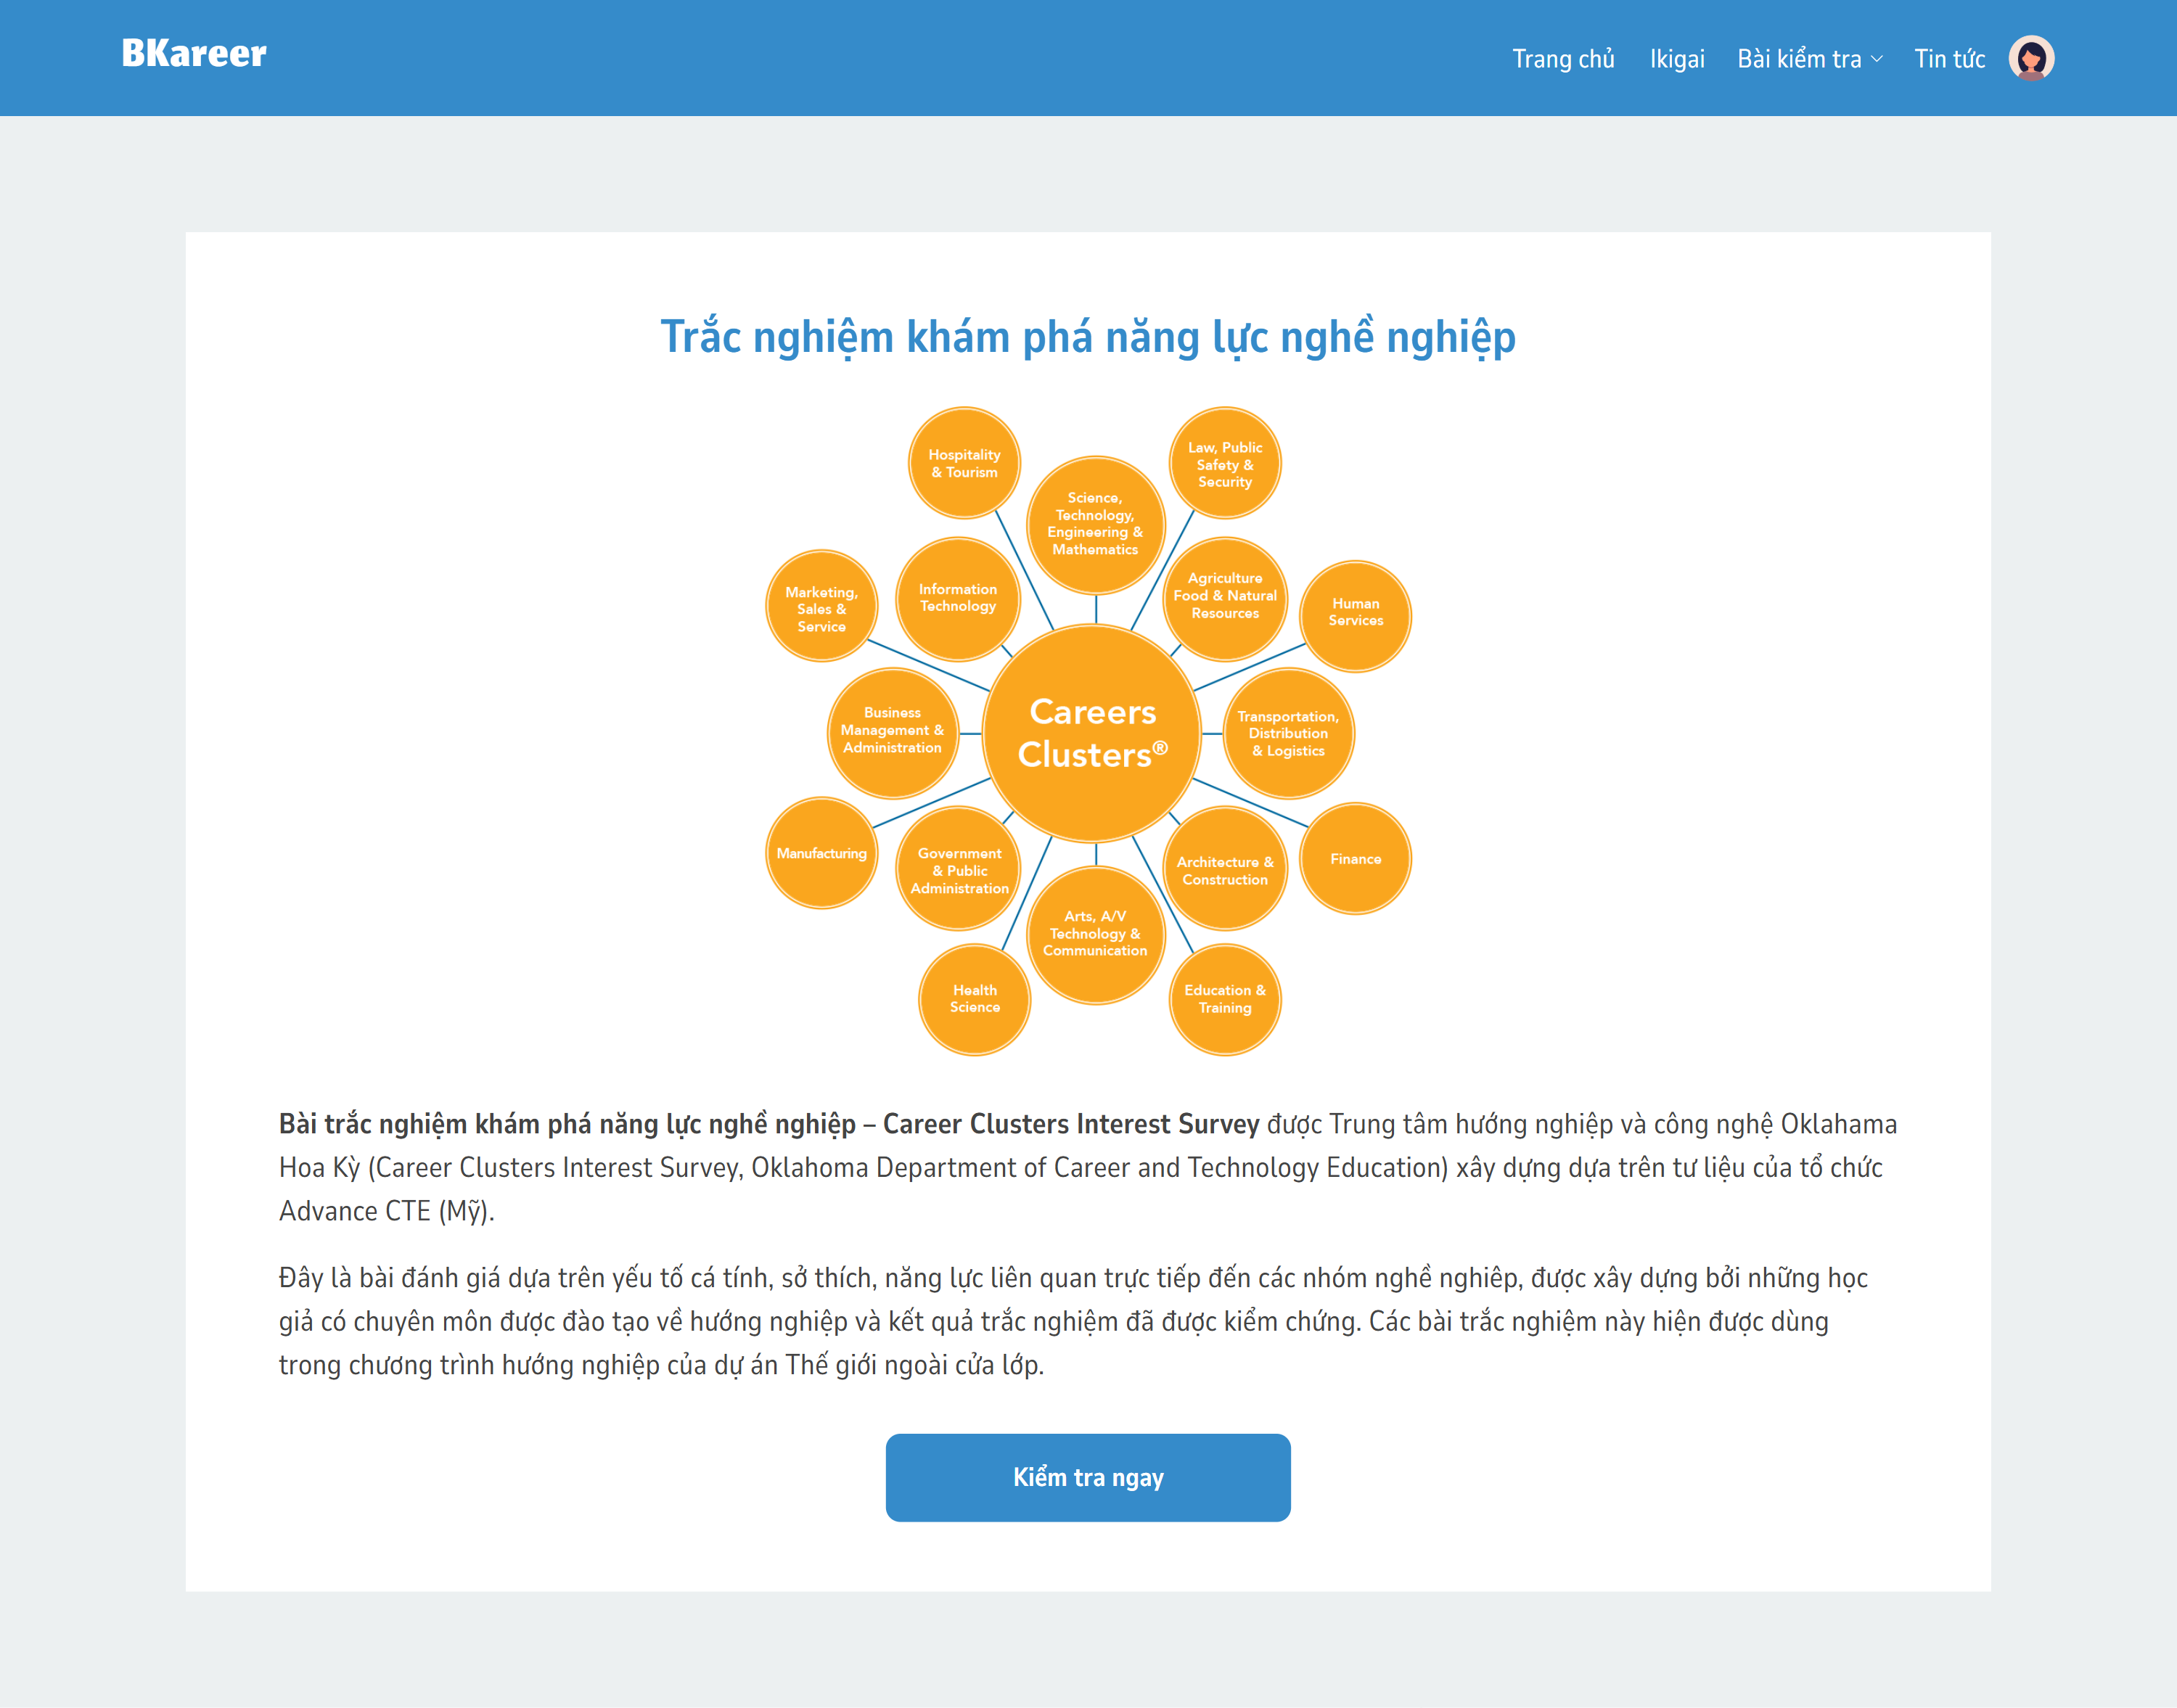
\includegraphics[width=0.8\textwidth]
    {images/chap5/ccDetail.png}
    \vspace{0.5cm}
    \caption{Trang giới thiệu trắc nghiệm khám phá năng lực nghề nghiệp}
\end{figure}

Các thành phần chính của trang giới thiệu trắc nghiệm khám phá năng lực nghề nghiệp:
\begin{itemize}
    \item Hình ảnh minh họa: Hình ảnh minh họa cho nội dung của trang giúp người dùng có thể hình dung sơ lược về trang.
    \item Phần giới thiệu: Phần giới thiệu có vai trò cung cấp thông tin cần thiết cho người dùng, giúp người dùng hiểu rõ hơn về mục đích, nội dung và thành phần bài kiểm tra, từ đó có sự chuẩn bị tốt hơn.
    \item Nút:
        \begin{itemize}
            \item Nút ``Bắt đầu ngay": Cho phép người dùng bắt đầu thực hiện bài kiểm tra ngay lập tức.
        \end{itemize}
\end{itemize}


%%%%%%%%%% Career Clustering Test %%%%%%%%%%
\subsection{Trang thực hiện trắc nghiệm khám phá năng lực nghề nghiệp}
Trang thực hiện trắc nghiệm khám phá năng lực nghề nghiệp là một giao diện được thiết kế để giúp người dùng đánh giá và hiểu rõ hơn về các kỹ năng, sở thích và năng lực của bản thân liên quan đến công việc. Bài trắc nghiệm khám phá năng lực nghề nghiệp bao gồm 16 ô, mỗi ô có 7 hoạt động, 5 phẩm chất cá nhân và 5 môn học yêu thích, cho phép người dùng chọn một hoặc nhiều lựa chọn miêu tả đúng nhất về bản thân. Thông qua các câu hỏi và lựa chọn, hệ thống sẽ cung cấp thông tin hữu ích để người dùng đưa ra quyết định về việc lựa chọn nghề nghiệp phù hợp.

Mục đích của trang thực hiện trắc nghiệm khám phá năng lực nghề nghiệp:
\begin{itemize}
    \item Xác định điểm mạnh: Nhận biết những kỹ năng, kiến thức và tố chất mà cá nhân sở hữu và làm tốt.
    \item Đánh giá tiềm năng: Đưa ra dự đoán về khả năng thành công trong các lĩnh vực nghề nghiệp khác nhau.
    \item Khám phá sở thích và hứng thú: Tìm hiểu về những hoạt động, lĩnh vực mà cá nhân cảm thấy hứng thú và yêu thích. Đề xuất các nghề nghiệp phù hợp với sở thích cá nhân để tạo động lực làm việc lâu dài.
    \item Hỗ trợ quá trình ra quyết định: Cung cấp thông tin khách quan, đa chiều về các ngành nghề, giúp cá nhân tự tin hơn trong việc đưa ra quyết định quan trọng về tương lai.
\end{itemize}

\begin{figure}[H]
    \centering
    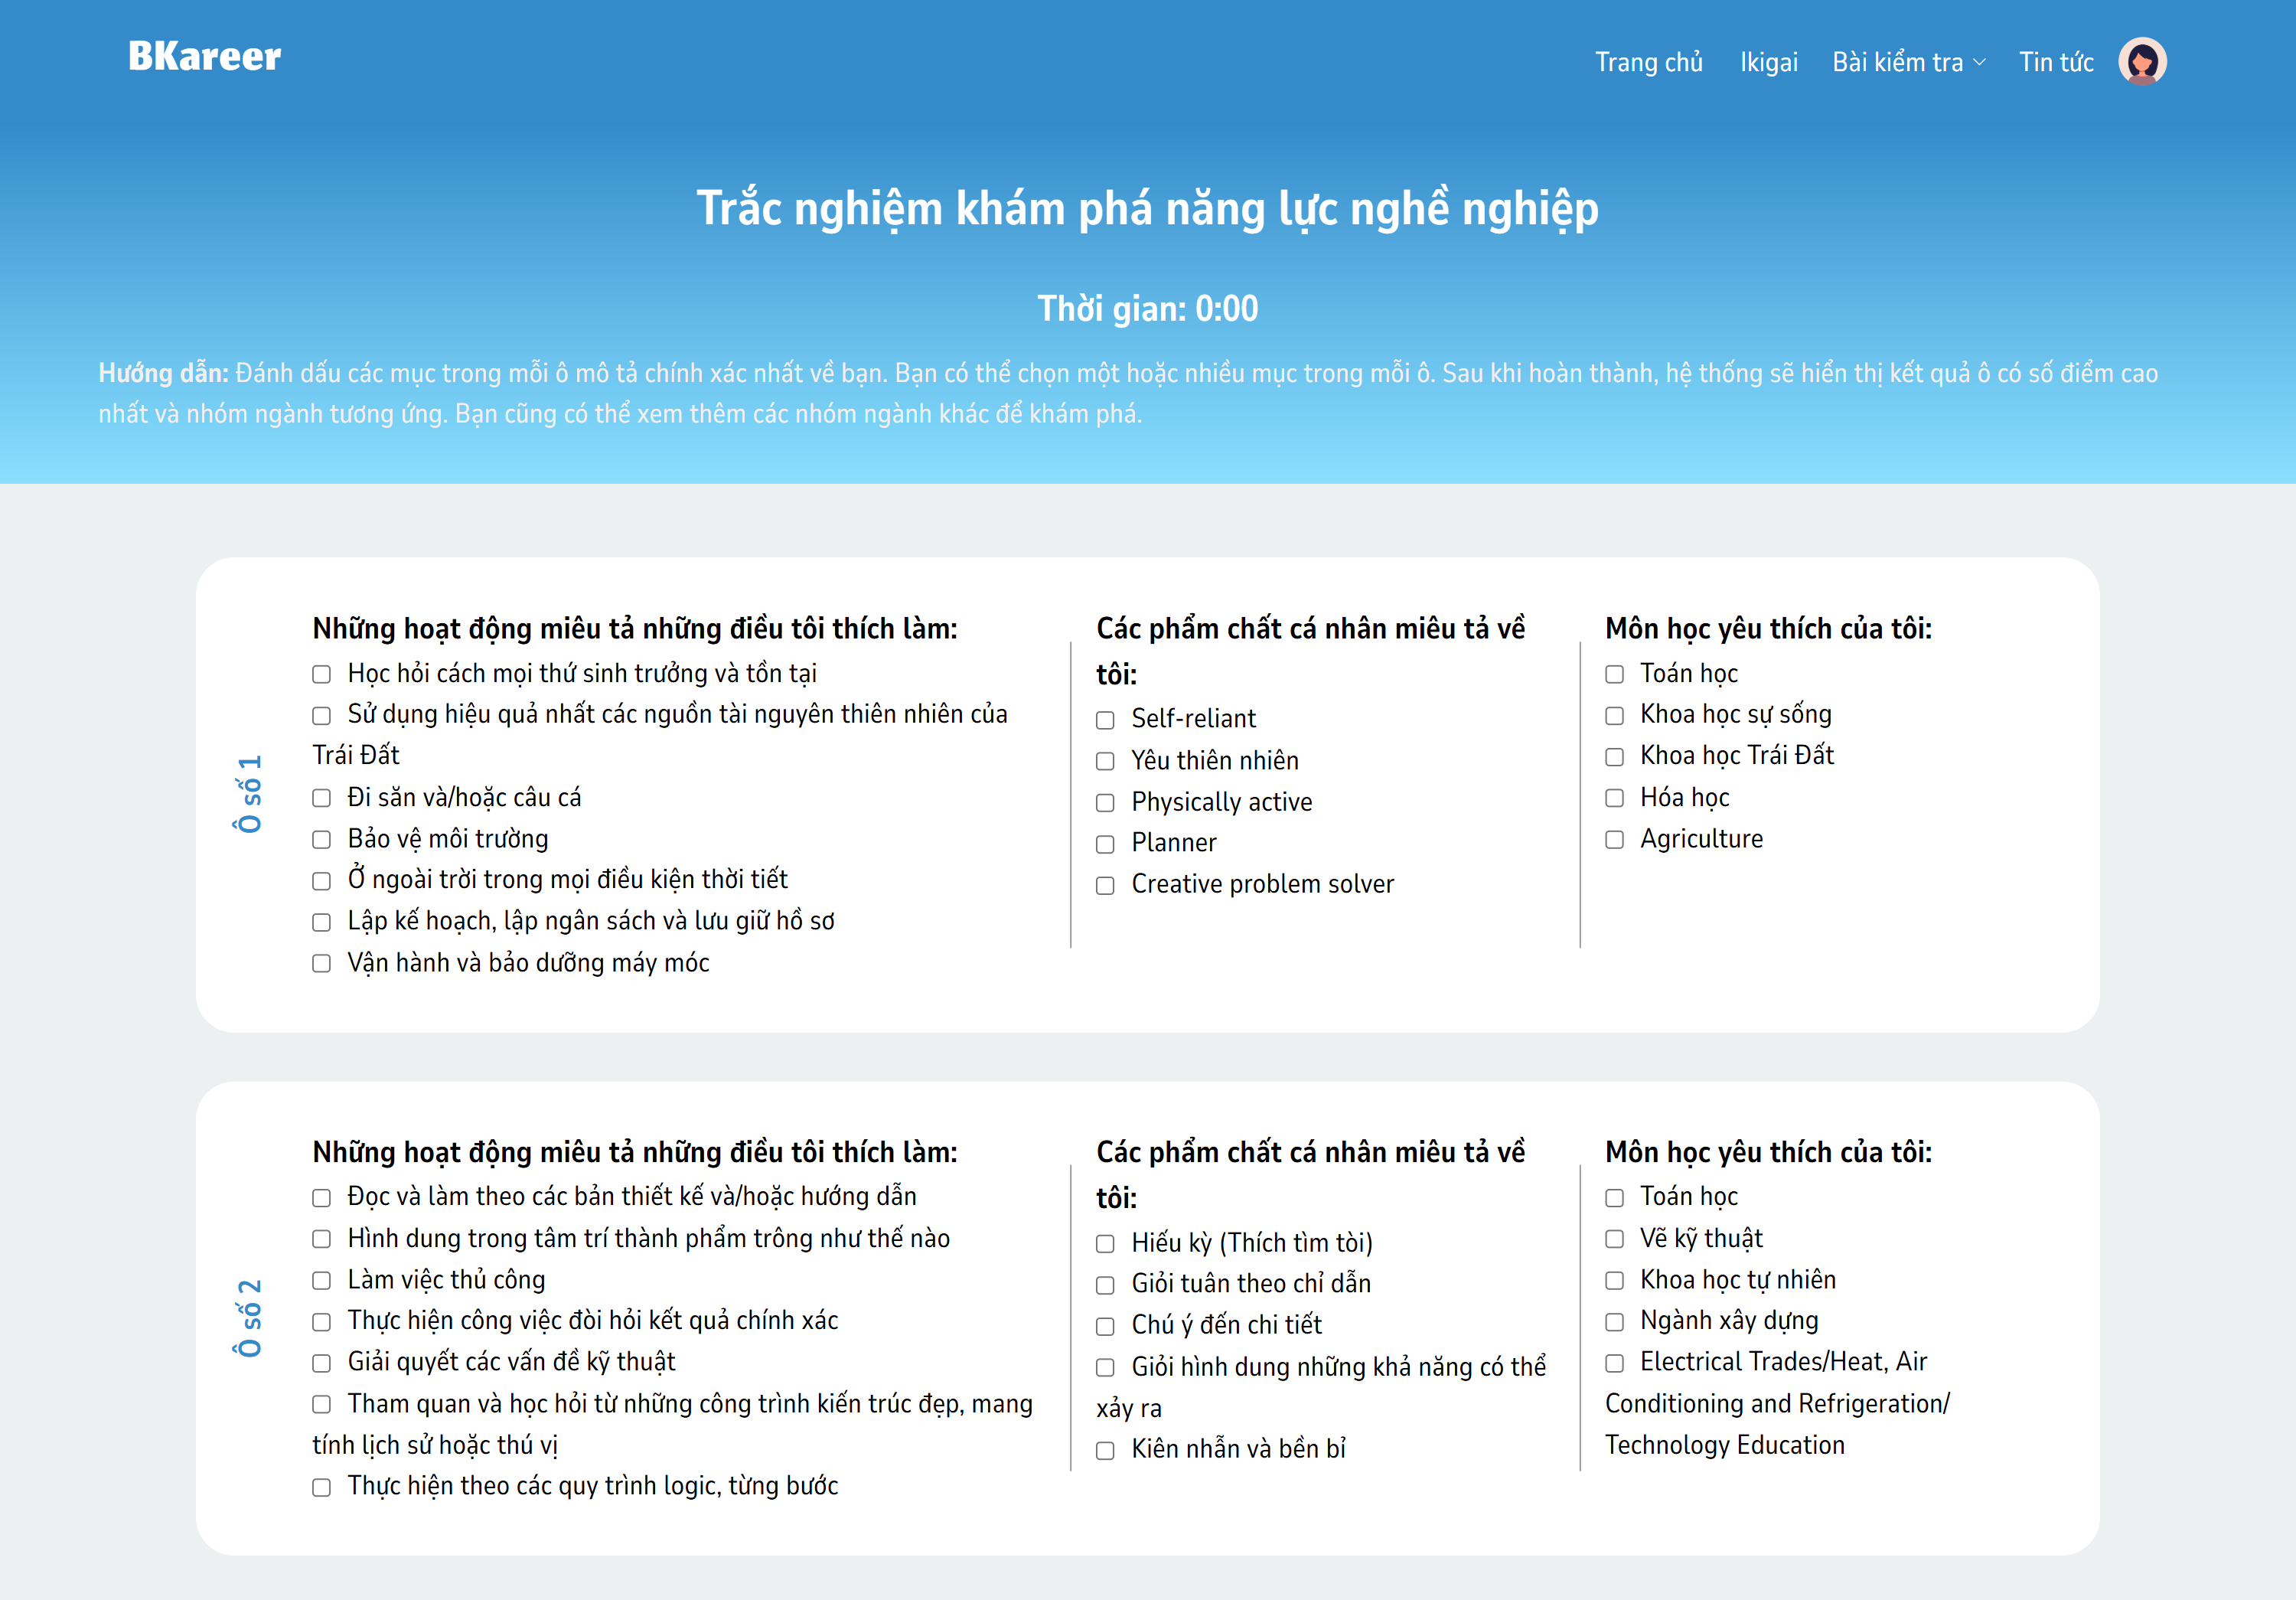
\includegraphics[width=0.8\textwidth]
    {images/chap5/career.png}
    \vspace{0.5cm}
    \caption{Trang thực hiện trắc nghiệm khám phá năng lực nghề nghiệp}
\end{figure}

Các thành phần chính của trang thực hiện trắc nghiệm khám phá năng lực nghề nghiệp:
\begin{itemize}
    \item Thanh tiến trình: Bao gồm đồng hồ đếm thời gian thực hiện bài kiểm tra.
    \item Hướng dẫn: Giúp người dùng hiểu rõ hơn về cách thức thực hiện bài kiểm tra để đạt được kết quả chính xác nhất.
    \item Phần giới thiệu: Phần giới thiệu có vai trò cung cấp thông tin cần thiết cho người dùng, giúp người dùng hiểu rõ hơn về mục đích, nội dung và thành phần bài kiểm tra, từ đó có sự chuẩn bị tốt hơn.
    \item Các ô câu hỏi: Mỗi ô bao gồm 3 phần và các lựa chọn cho mỗi phần, cho phép người dùng chọn các lựa chọn mô tả đúng về bản thân mình, và có thể thay đổi sau khi lựa chọn.
    \item Nút:
        \begin{itemize}
            \item Nút ``Quay về nhập kết quả": Cho phép người dùng kết thúc kiểm tra sau khi đã hoàn thành và quay trở về trang nhập kết quả kiểm tra định hướng ngành nghề, hệ thống sẽ tự ghi nhận và điền kết quả vào phần trắc nghiệm MBTI tương ứng.
            \item Nút ``Xem kết quả": Hiển thị giao diện thông báo kết quả cho người dùng.
        \end{itemize}
\end{itemize}


%%%%%%%%%% Feedback Result %%%%%%%%%%
% \subsection{Trang đánh giá và nhận xét}
% Trang đánh giá và nhận xét là một phần không thể thiếu trên hầu hết các hệ thống, đặc biệt là những hệ thống cung cấp sản phẩm, dịch vụ hoặc nội dung. Đây là nơi người dùng có thể chia sẻ ý kiến, đánh giá và đóng góp của mình về sản phẩm, dịch vụ hoặc trải nghiệm để hệ thống cải tiến và hoàn thiện hơn.

% \begin{figure}[H]
%     \centering
%     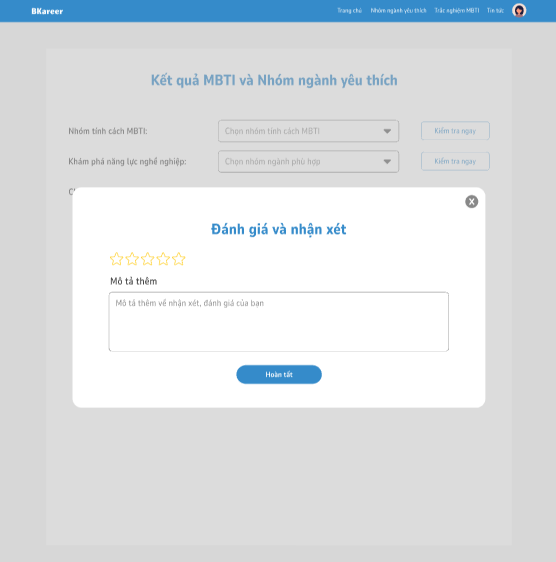
\includegraphics[width=0.8\linewidth]{images/feedback.png}
%     \vspace{0.6cm}
%     \caption{Đánh giá và nhận xét}
% \end{figure}


%%%%%%%%%% IQ Detail %%%%%%%%%%
\subsection{Trang giới thiệu trắc nghiệm IQ}
Trang giới thiệu trắc nghiệm IQ thường có vai trò cung cấp thông tin tổng quan về công cụ đánh giá này. Nó giúp người đọc hiểu rõ mục đích, cách thức hoạt động, độ tin cậy và những ứng dụng của trắc nghiệm IQ.

Mục đích của trang giới thiệu trắc nghiệm IQ:
\begin{itemize}
    \item Giải thích khái niệm IQ: Định nghĩa rõ ràng về chỉ số IQ, cách tính toán và ý nghĩa của nó.
    \item Giới thiệu về trắc nghiệm IQ: Mô tả mục đích, cấu trúc và nội dung của trắc nghiệm.
    \item Hướng dẫn thực hiện trắc nghiệm: Hướng dẫn chi tiết các bước để tham gia làm bài trắc nghiệm và mô tả môi trường làm bài lý tưởng để đạt kết quả tốt nhất.
\end{itemize}

\begin{figure}[H]
    \centering
    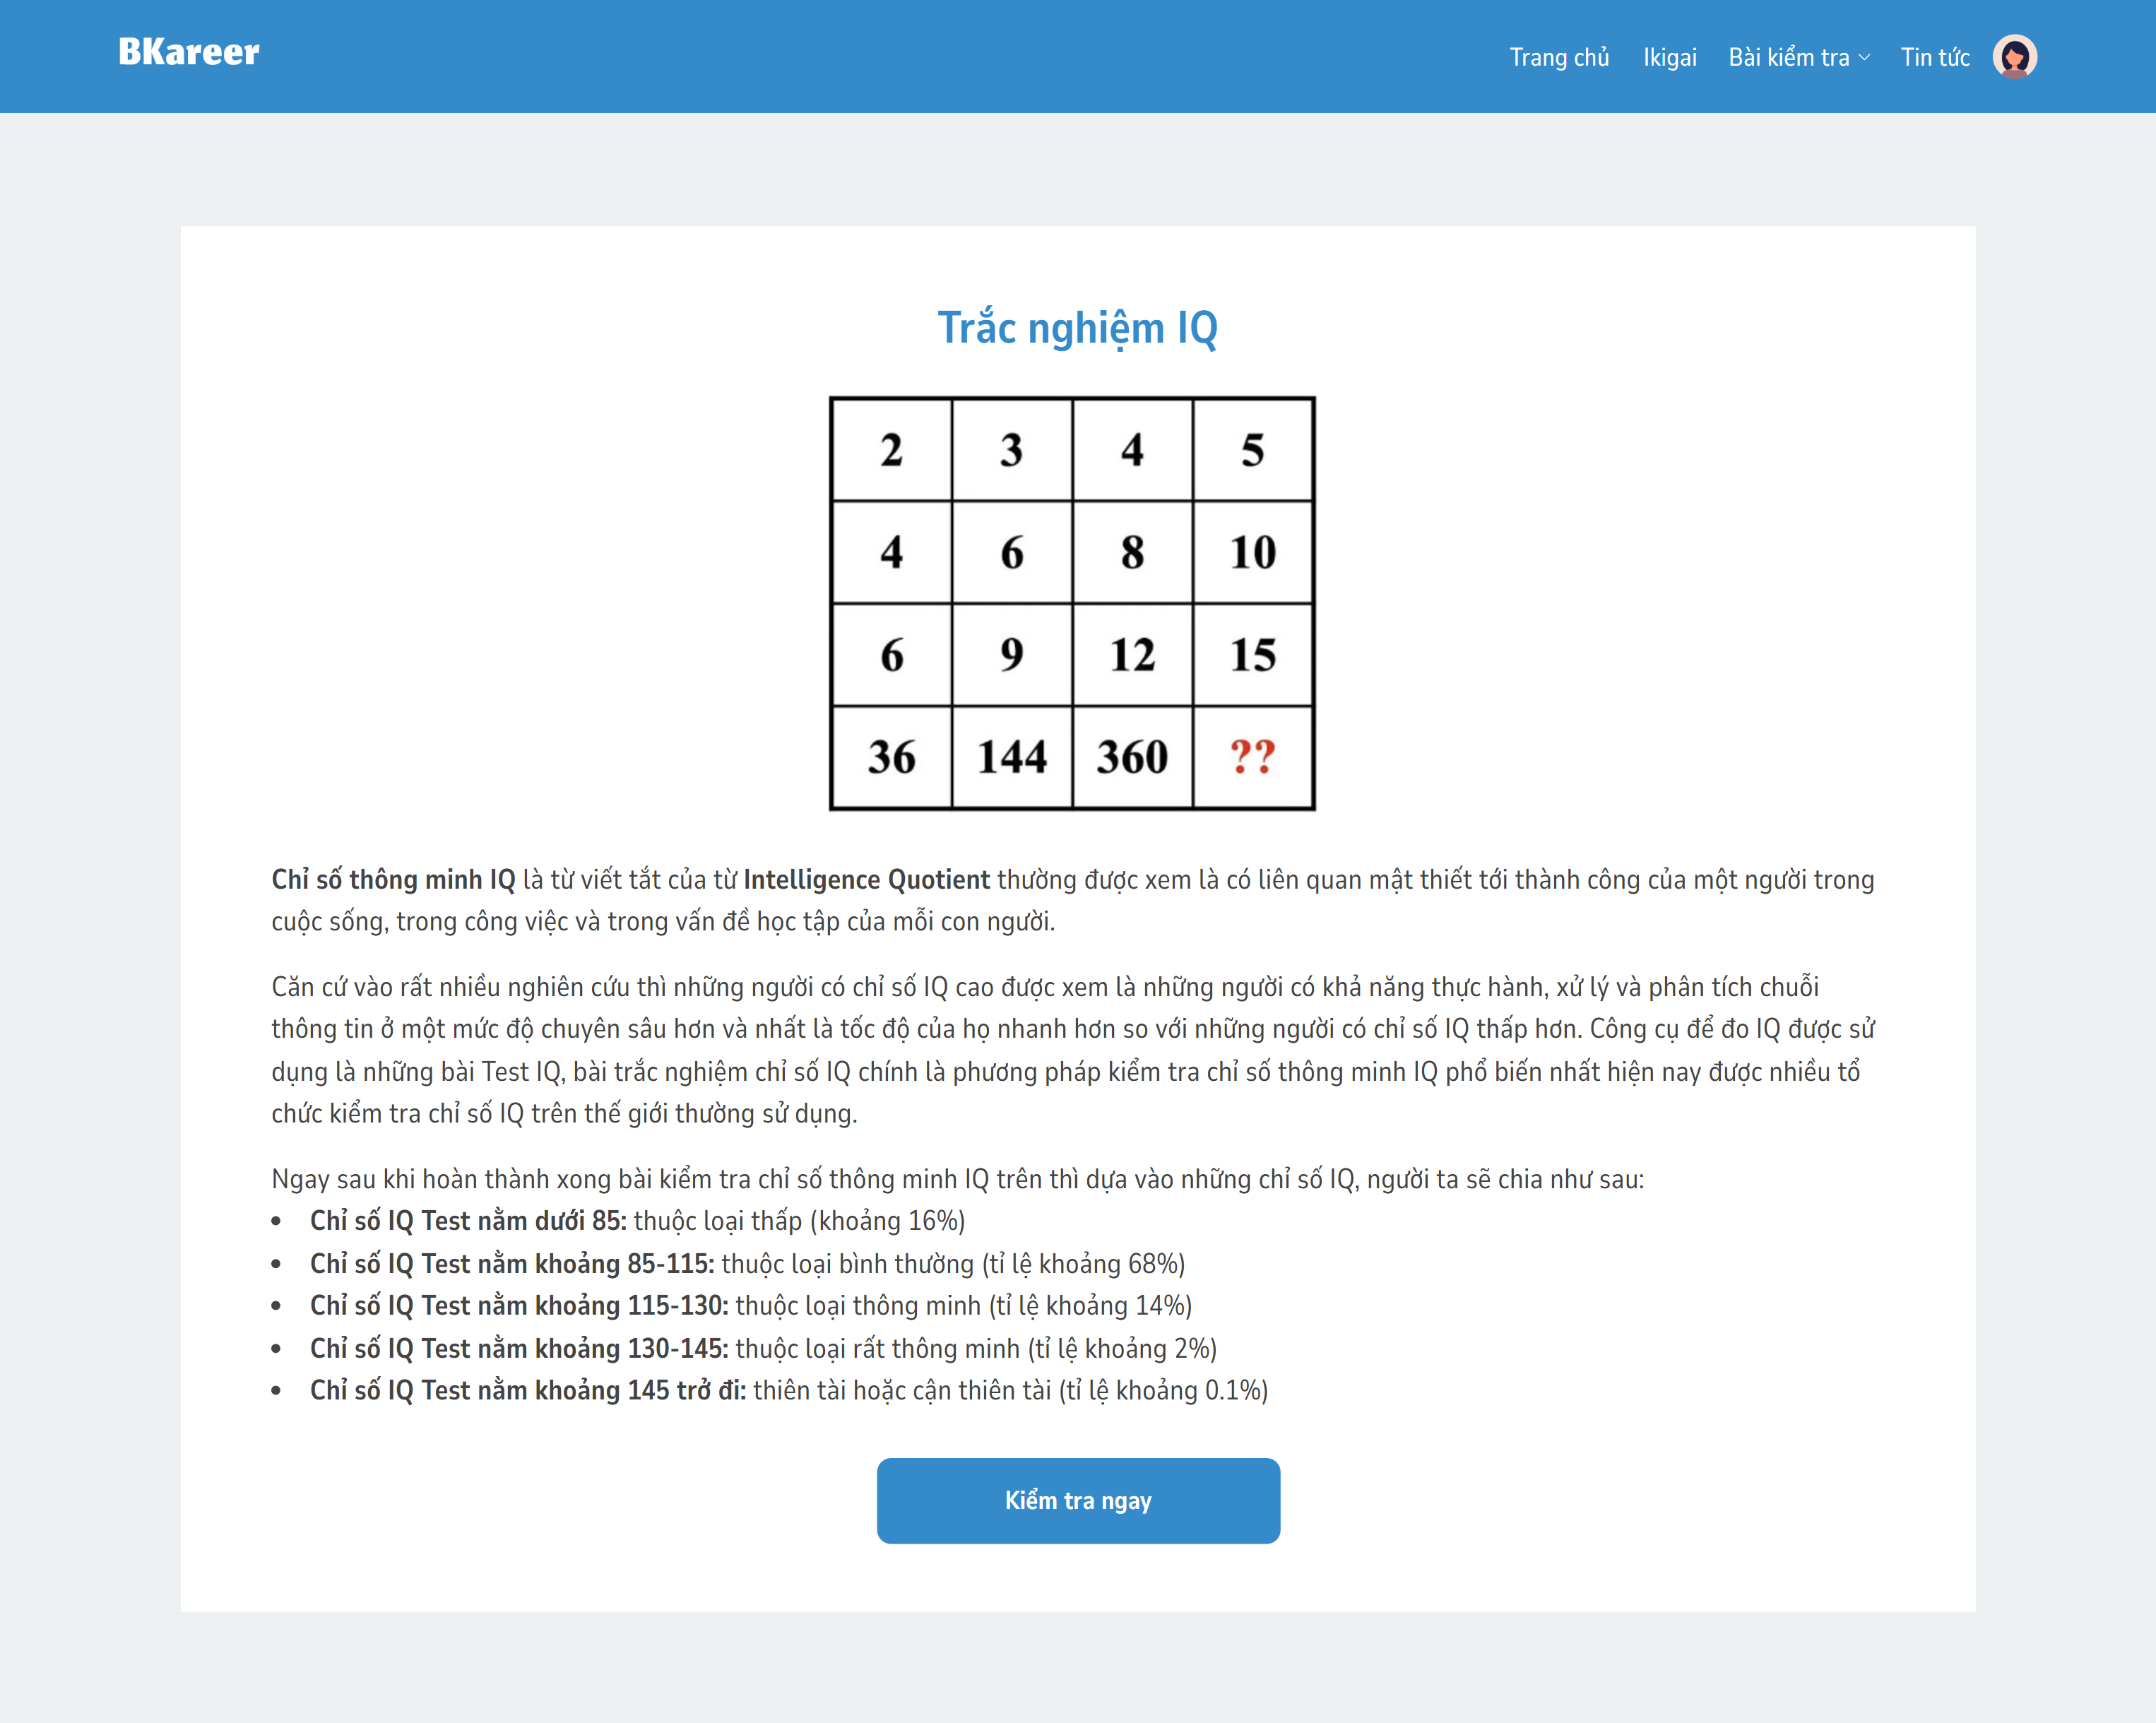
\includegraphics[width=0.8\textwidth]
    {images/chap5/iqDetail.png}
    \vspace{0.5cm}
    \caption{Trang giới thiệu trắc nghiệm IQ}
\end{figure}

Các thành phần chính của trang giới thiệu trắc nghiệm IQ:
\begin{itemize}
    \item Hình ảnh minh họa: Hình ảnh minh họa cho nội dung của trang giúp người dùng có thể hình dung sơ lược về trang.
    \item Phần giới thiệu: Phần giới thiệu có vai trò cung cấp thông tin cần thiết cho người dùng, giúp người dùng hiểu rõ hơn về mục đích, nội dung và thành phần bài kiểm tra, từ đó có sự chuẩn bị tốt hơn.
    \item Nút:
        \begin{itemize}
            \item Nút ``Kiểm tra ngay": Cho phép người dùng chuyển đến trang kiểm tra để bắt đầu thực hiện bài kiểm tra ngay lập tức.
        \end{itemize}
\end{itemize}


%%%%%%%%%% IQ Test %%%%%%%%%%
\subsection{Trang thực hiện trắc nghiệm IQ}
Trang thực hiện trắc nghiệm IQ là một nền tảng được thiết kế để đánh giá chỉ số thông minh (IQ) của người dùng. Thông qua các câu hỏi đa dạng, bao gồm các bài toán logic, hình ảnh, ngôn ngữ, trang web này sẽ giúp người dùng xác định mức độ thông minh tương đối so với dân số.

Mục đích của trang thực hiện trắc nghiệm IQ:
\begin{itemize}
    \item Tìm hiểu bản thân: Giúp người dùng hiểu rõ hơn về khả năng tư duy, trí thông minh của mình.
    \item Đánh giá sự phát triển: So sánh kết quả qua các lần làm bài để theo dõi sự tiến bộ về khả năng tư duy.
    \item Khám phá tiềm năng: Phát hiện ra những điểm mạnh, điểm yếu trong tư duy để khai thác tối đa khả năng của bản thân.
    \item Tìm kiếm phương pháp học tập hiệu quả: Dựa trên kết quả trắc nghiệm, người dùng có thể tìm ra phương pháp học tập phù hợp với bản thân.
\end{itemize}

\begin{figure}[H]
    \centering
    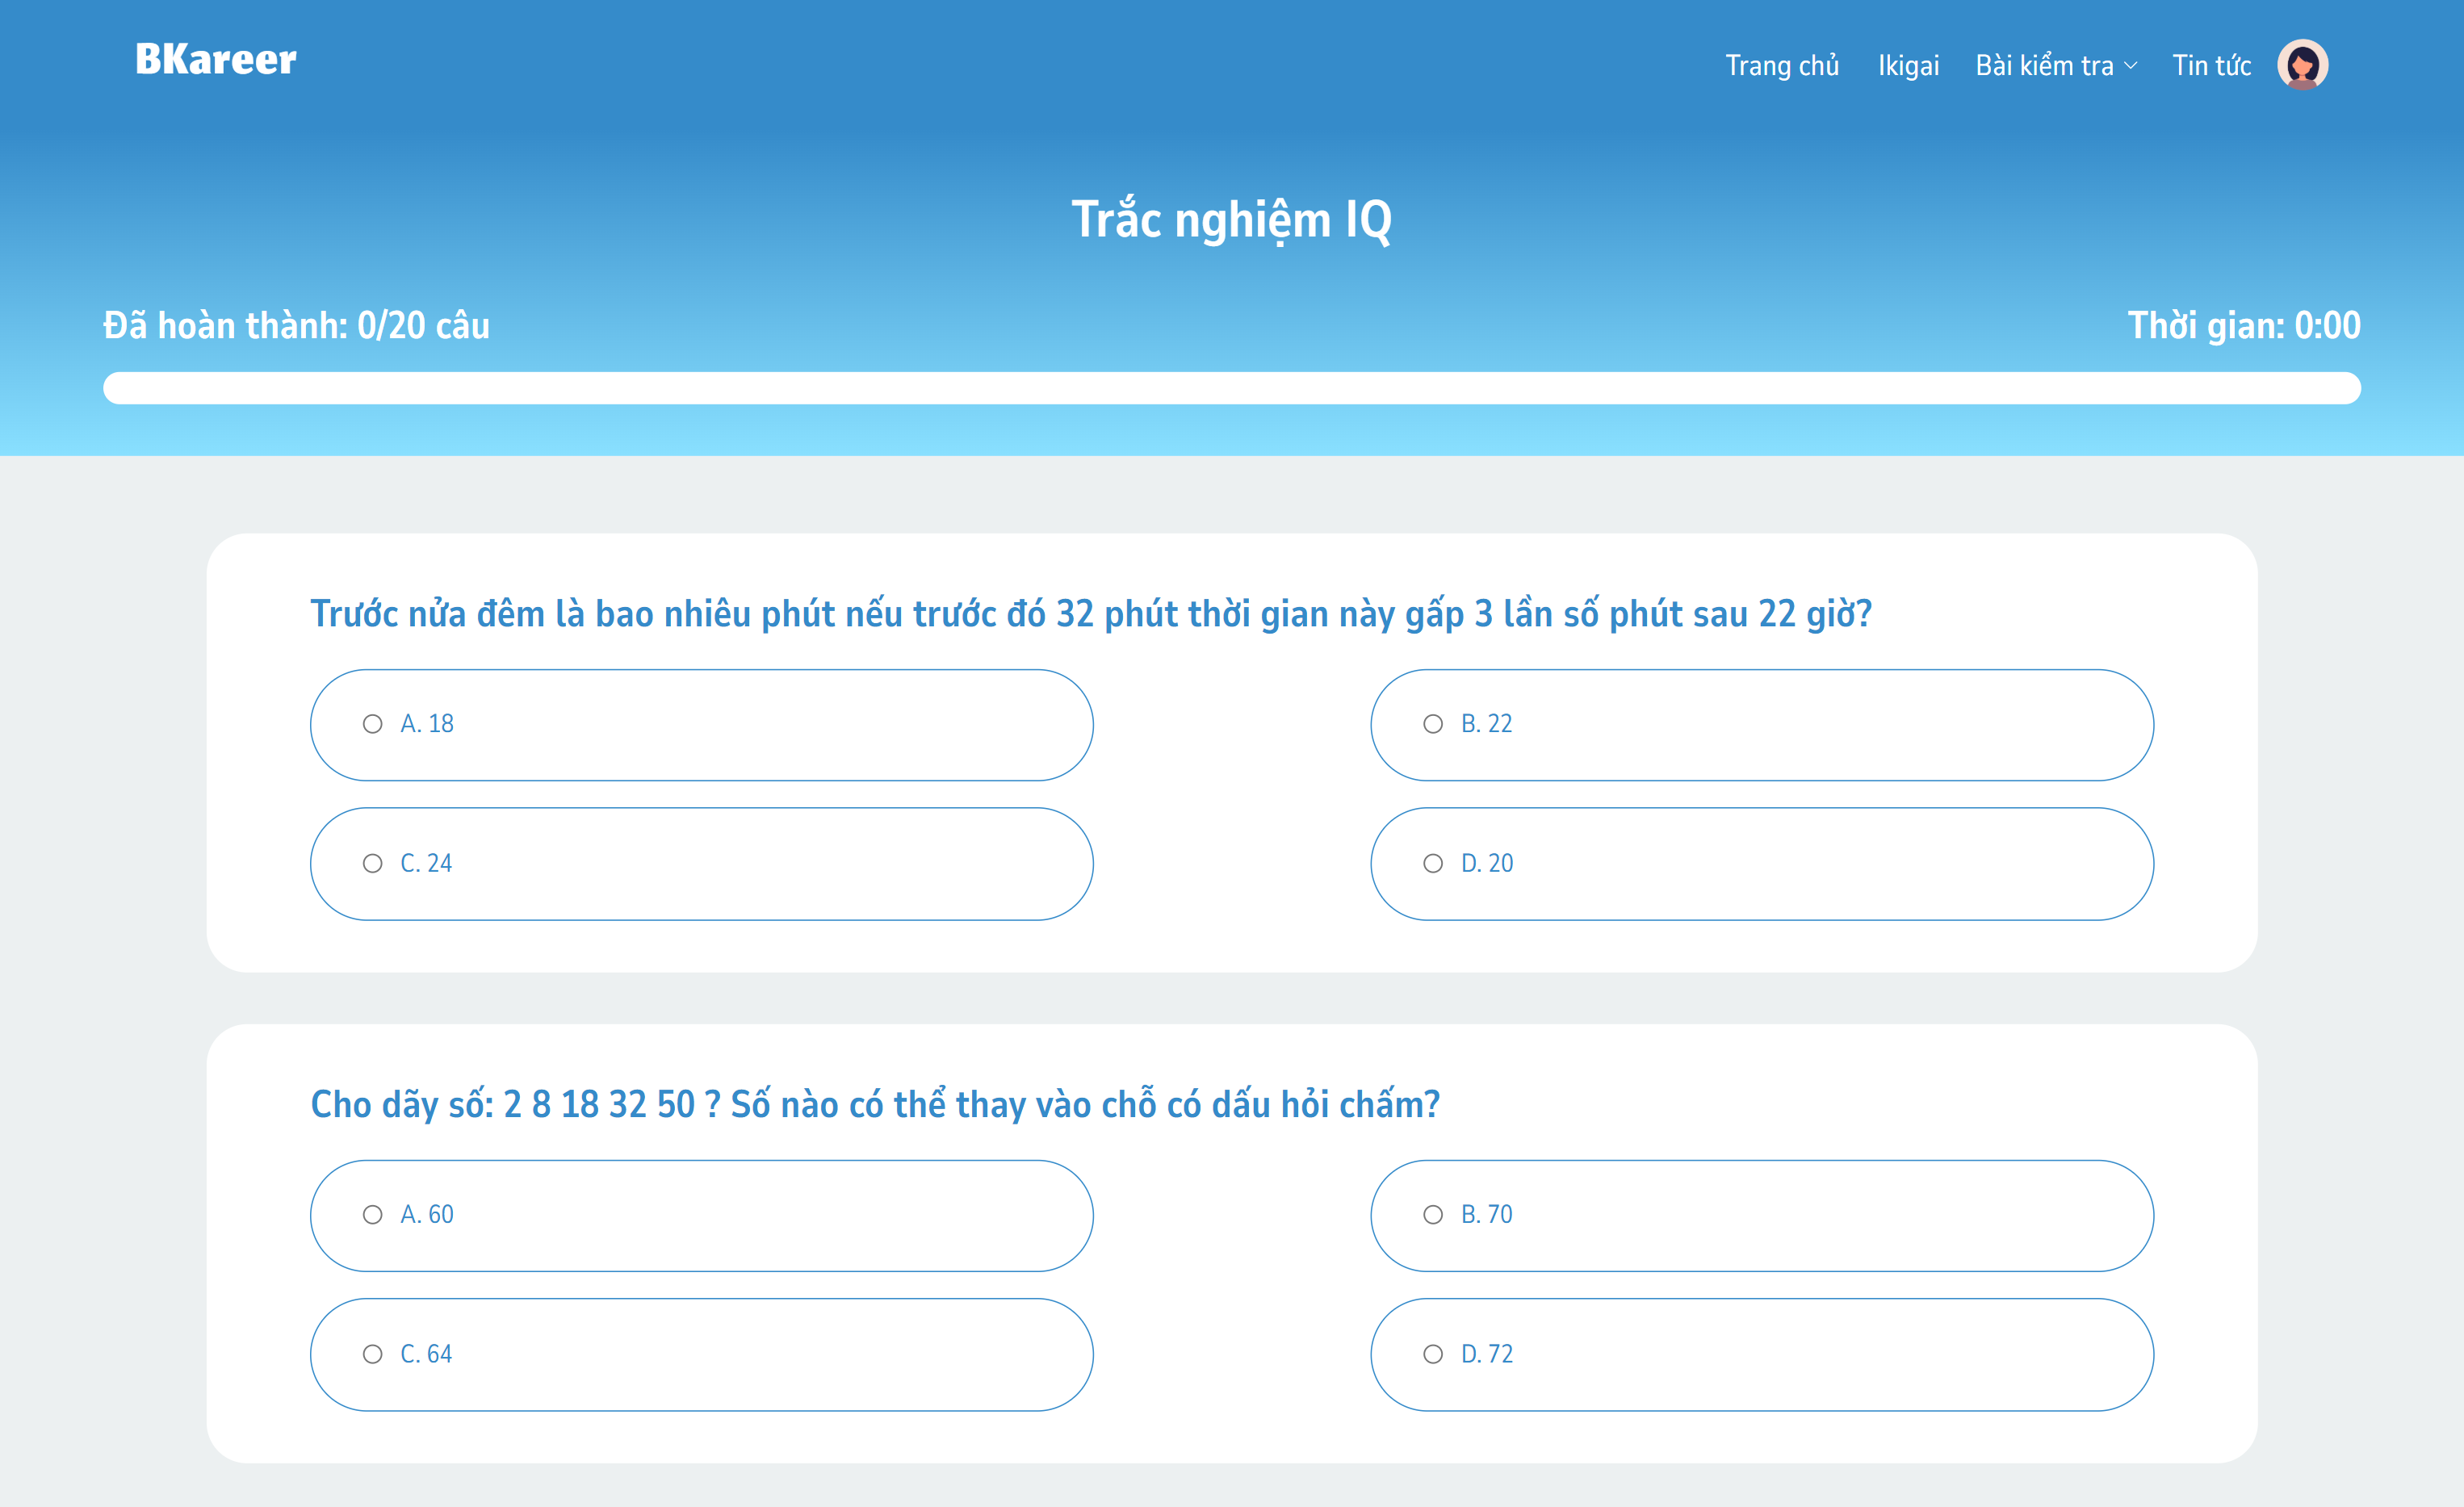
\includegraphics[width=0.8\textwidth]
    {images/chap5/iq.png}
    \vspace{0.5cm}
    \caption{Trang thực hiện trắc nghiệm IQ}
\end{figure}

Các thành phần chính của trang thực hiện trắc nghiệm IQ:
\begin{itemize}
    \item Thanh tiến trình: Bao gồm tiến độ hoàn thành bài kiểm tra và đồng hồ đếm thời gian thực hiện bài kiểm tra.
    \item Các khối câu hỏi: Mỗi khối bao gồm 1 câu hỏi và 4 đáp án, cho phép người dùng chọn 1 trong 4 đáp án, và có thể thay đổi sau khi lựa chọn.
    \item Nút:
        \begin{itemize}
            \item Nút ``Xem kết quả": Hiển thị giao diện thông báo kết quả cho người dùng.
        \end{itemize}
\end{itemize}


%%%%%%%%%% EQ Detail %%%%%%%%%%
\subsection{Trang giới thiệu trắc nghiệm EQ}
Trang giới thiệu trắc nghiệm EQ là một phần của hệ thống, cung cấp thông tin chi tiết về một công cụ đánh giá giúp người dùng xác định chỉ số cảm xúc (EQ - Emotional Quotient) của bản thân, là khả năng nhận biết, hiểu và quản lý cảm xúc của bản thân và người khác.

Mục đích của trang giới thiệu trắc nghiệm EQ:
\begin{itemize}
    \item Giải thích về EQ: Cung cấp định nghĩa rõ ràng về EQ, tầm quan trọng của EQ trong cuộc sống và công việc.
    \item Giới thiệu về trắc nghiệm: Giải thích cách thức hoạt động của trắc nghiệm, loại câu hỏi và cách tính điểm.
    \item Nêu rõ lợi ích của việc xác định EQ: Giúp người dùng hiểu rõ hơn về điểm mạnh, điểm yếu trong việc quản lý cảm xúc của mình, từ đó cải thiện các mối quan hệ xã hội, nâng cao hiệu quả công việc và cuộc sống.
\end{itemize}

\begin{figure}[H]
    \centering
    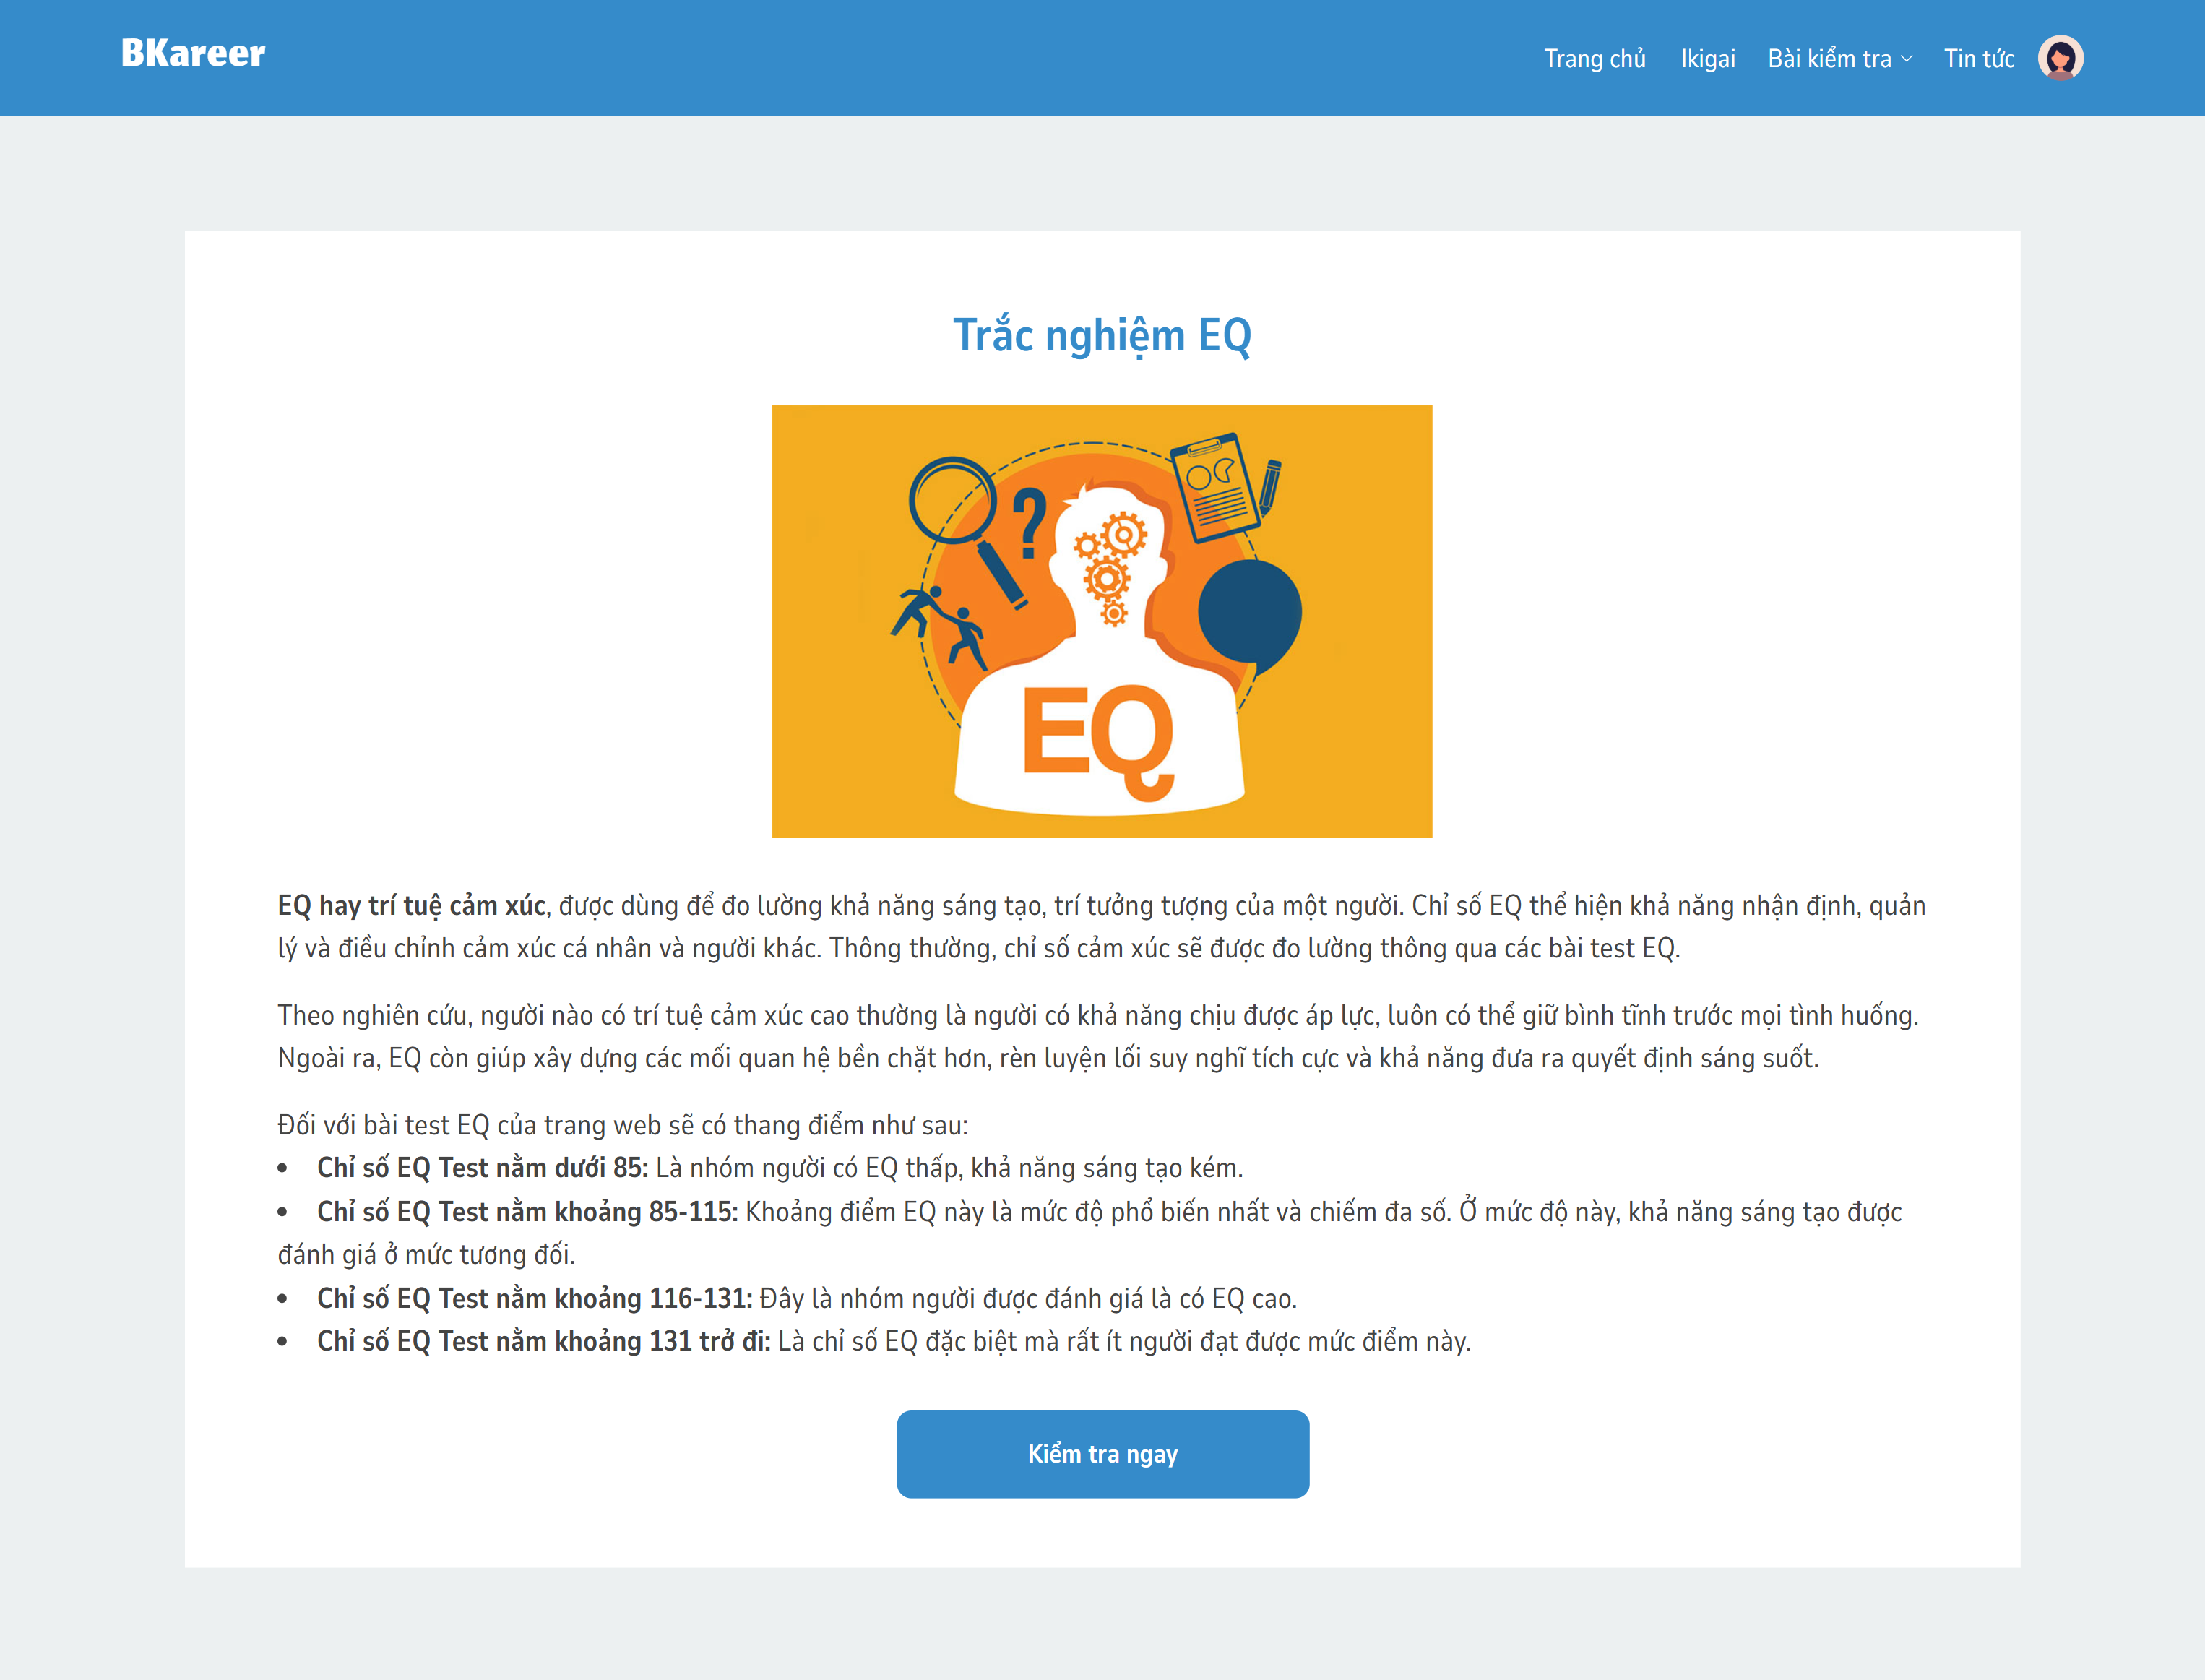
\includegraphics[width=0.8\textwidth]
    {images/chap5/eqDetail.png}
    \vspace{0.5cm}
    \caption{Trang giới thiệu trắc nghiệm EQ}
\end{figure}

Các thành phần chính của trang giới thiệu trắc nghiệm EQ:
\begin{itemize}
    \item Hình ảnh minh họa: Hình ảnh minh họa cho nội dung của trang giúp người dùng có thể hình dung sơ lược về trang.
    \item Phần giới thiệu: Phần giới thiệu có vai trò cung cấp thông tin cần thiết cho người dùng, giúp người dùng hiểu rõ hơn về mục đích, nội dung và thành phần bài kiểm tra, từ đó có sự chuẩn bị tốt hơn.
    \item Nút:
        \begin{itemize}
            \item Nút ``Kiểm tra ngay": Cho phép người dùng chuyển đến trang kiểm tra để bắt đầu thực hiện bài kiểm tra ngay lập tức.
        \end{itemize}
\end{itemize}


%%%%%%%%%% EQ Test %%%%%%%%%%
\subsection{Trang thực hiện trắc nghiệm EQ}
Trang thực hiện trắc nghiệm EQ là một nền tảng trực tuyến được thiết kế để giúp người dùng đánh giá chỉ số cảm xúc (Emotional Quotient - EQ) của bản thân. EQ là khả năng nhận biết, hiểu và quản lý cảm xúc của chính mình cũng như của người khác.

Mục đích của trang thực hiện trắc nghiệm EQ:
\begin{itemize}
    \item Đánh giá chỉ số EQ: Cung cấp một công cụ để người dùng tự đánh giá khả năng cảm xúc của mình.
    \item Cải thiện kỹ năng giao tiếp: Đưa ra những gợi ý để phát triển các kỹ năng giao tiếp, xây dựng mối quan hệ.
    \item Nâng cao hiệu quả công việc: Giúp người dùng hiểu rõ hơn về cách làm việc nhóm, giải quyết xung đột.
    \item Phát triển cá nhân: Hỗ trợ người dùng phát triển toàn diện hơn về mặt cảm xúc.
\end{itemize}

\begin{figure}[H]
    \centering
    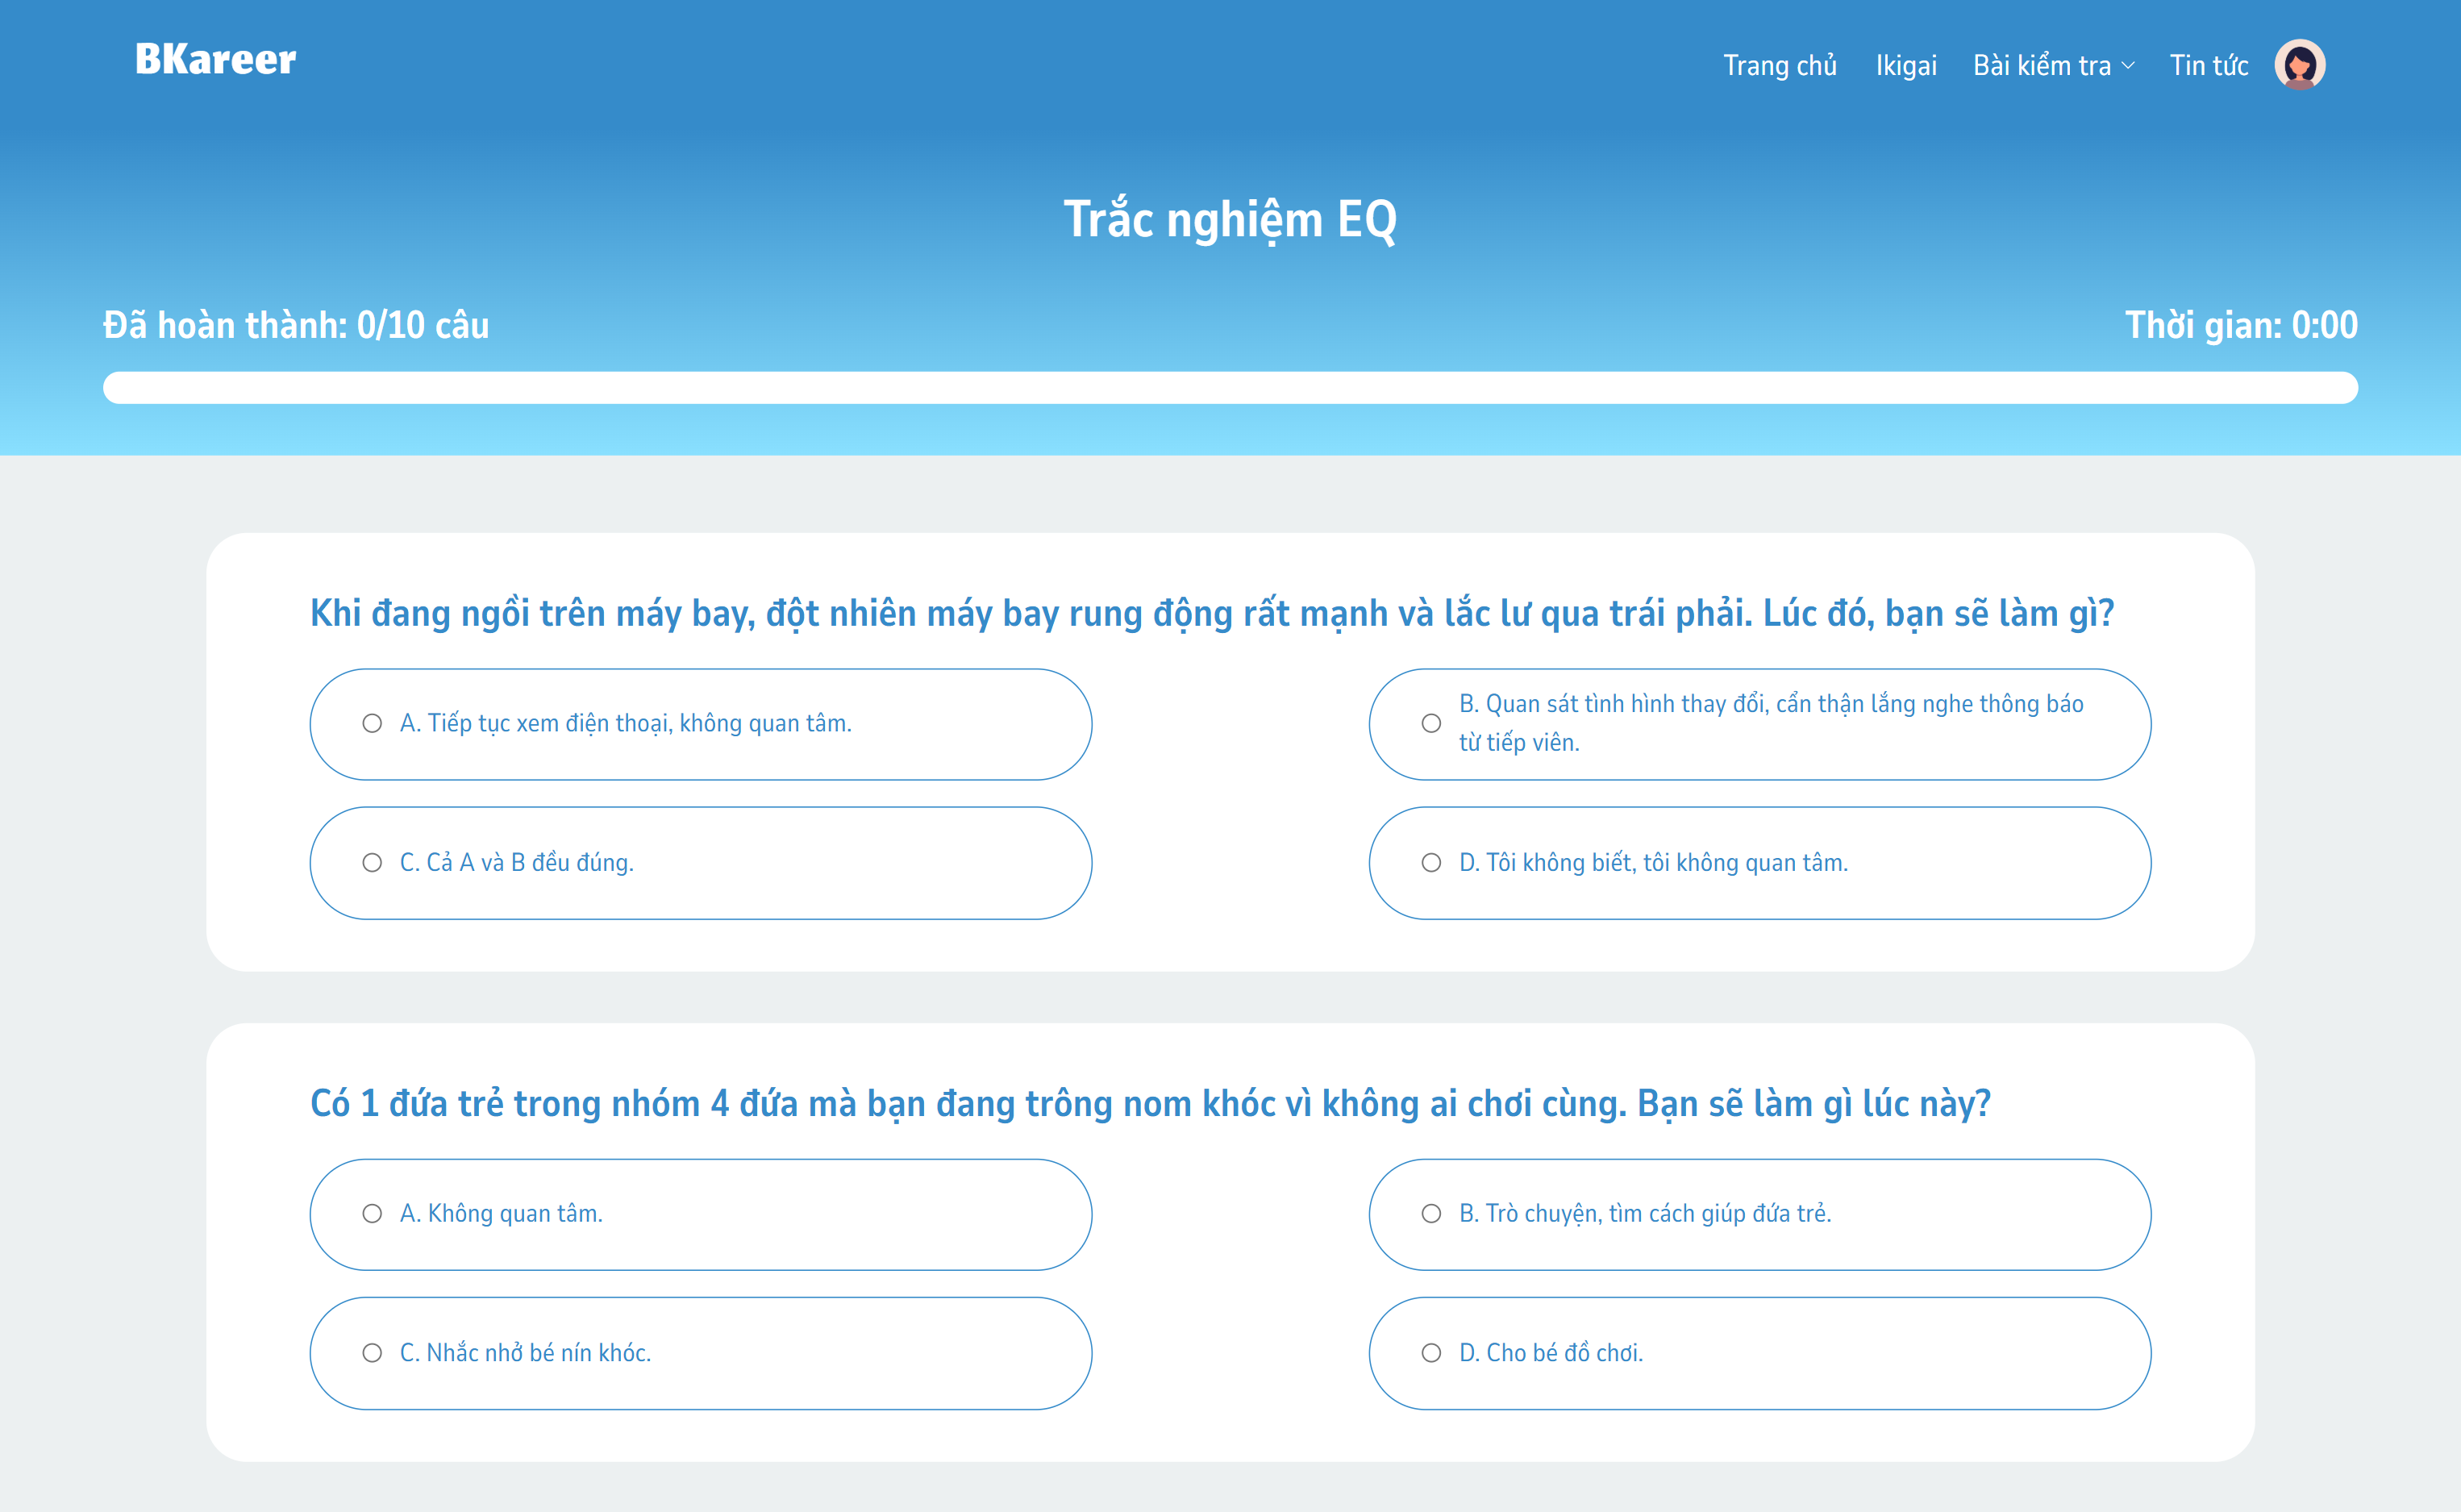
\includegraphics[width=0.8\textwidth]
    {images/chap5/eq.png}
    \vspace{0.5cm}
    \caption{Trang thực hiện trắc nghiệm EQ}
\end{figure}

Các thành phần chính của trang thực hiện trắc nghiệm EQ:
\begin{itemize}
    \item Thanh tiến trình: Bao gồm tiến độ hoàn thành bài kiểm tra và đồng hồ đếm thời gian thực hiện bài kiểm tra.
    \item Các khối câu hỏi: Mỗi khối bao gồm 1 câu hỏi và 4 đáp án, cho phép người dùng chọn 1 trong 4 đáp án, và có thể thay đổi sau khi lựa chọn.
    \item Nút:
        \begin{itemize}
            \item Nút ``Xem kết quả": Hiển thị giao diện thông báo kết quả cho người dùng.
        \end{itemize}
\end{itemize}


%%%%%%%%%% Left Right Brain Detail %%%%%%%%%%
\subsection{Trang giới thiệu trắc nghiệm não trái - não phải}
Trang giới thiệu trắc nghiệm não trái - não phải là một phần của hệ thống, cung cấp thông tin chi tiết về một công cụ đánh giá giúp người dùng xác định xem họ có xu hướng sử dụng não trái (logic, phân tích) hay não phải (sáng tạo, trực giác) nhiều hơn.

Mục đích của trang giới thiệu trắc nghiệm não trái - não phải:
\begin{itemize}
    \item Giải thích về não trái và não phải: Trang web sẽ cung cấp định nghĩa rõ ràng về hai bán cầu não, các chức năng chính của mỗi bán cầu và cách chúng hoạt động.
    \item Giới thiệu về trắc nghiệm: Giải thích cách thức hoạt động của trắc nghiệm, loại câu hỏi và cách tính điểm.
    \item Nêu rõ lợi ích của việc xác định thiên hướng não: Giúp người dùng hiểu rõ hơn về cách tư duy, học tập và làm việc của bản thân, từ đó tìm ra phương pháp phù hợp để phát triển các kỹ năng.
\end{itemize}

\begin{figure}[H]
    \centering
    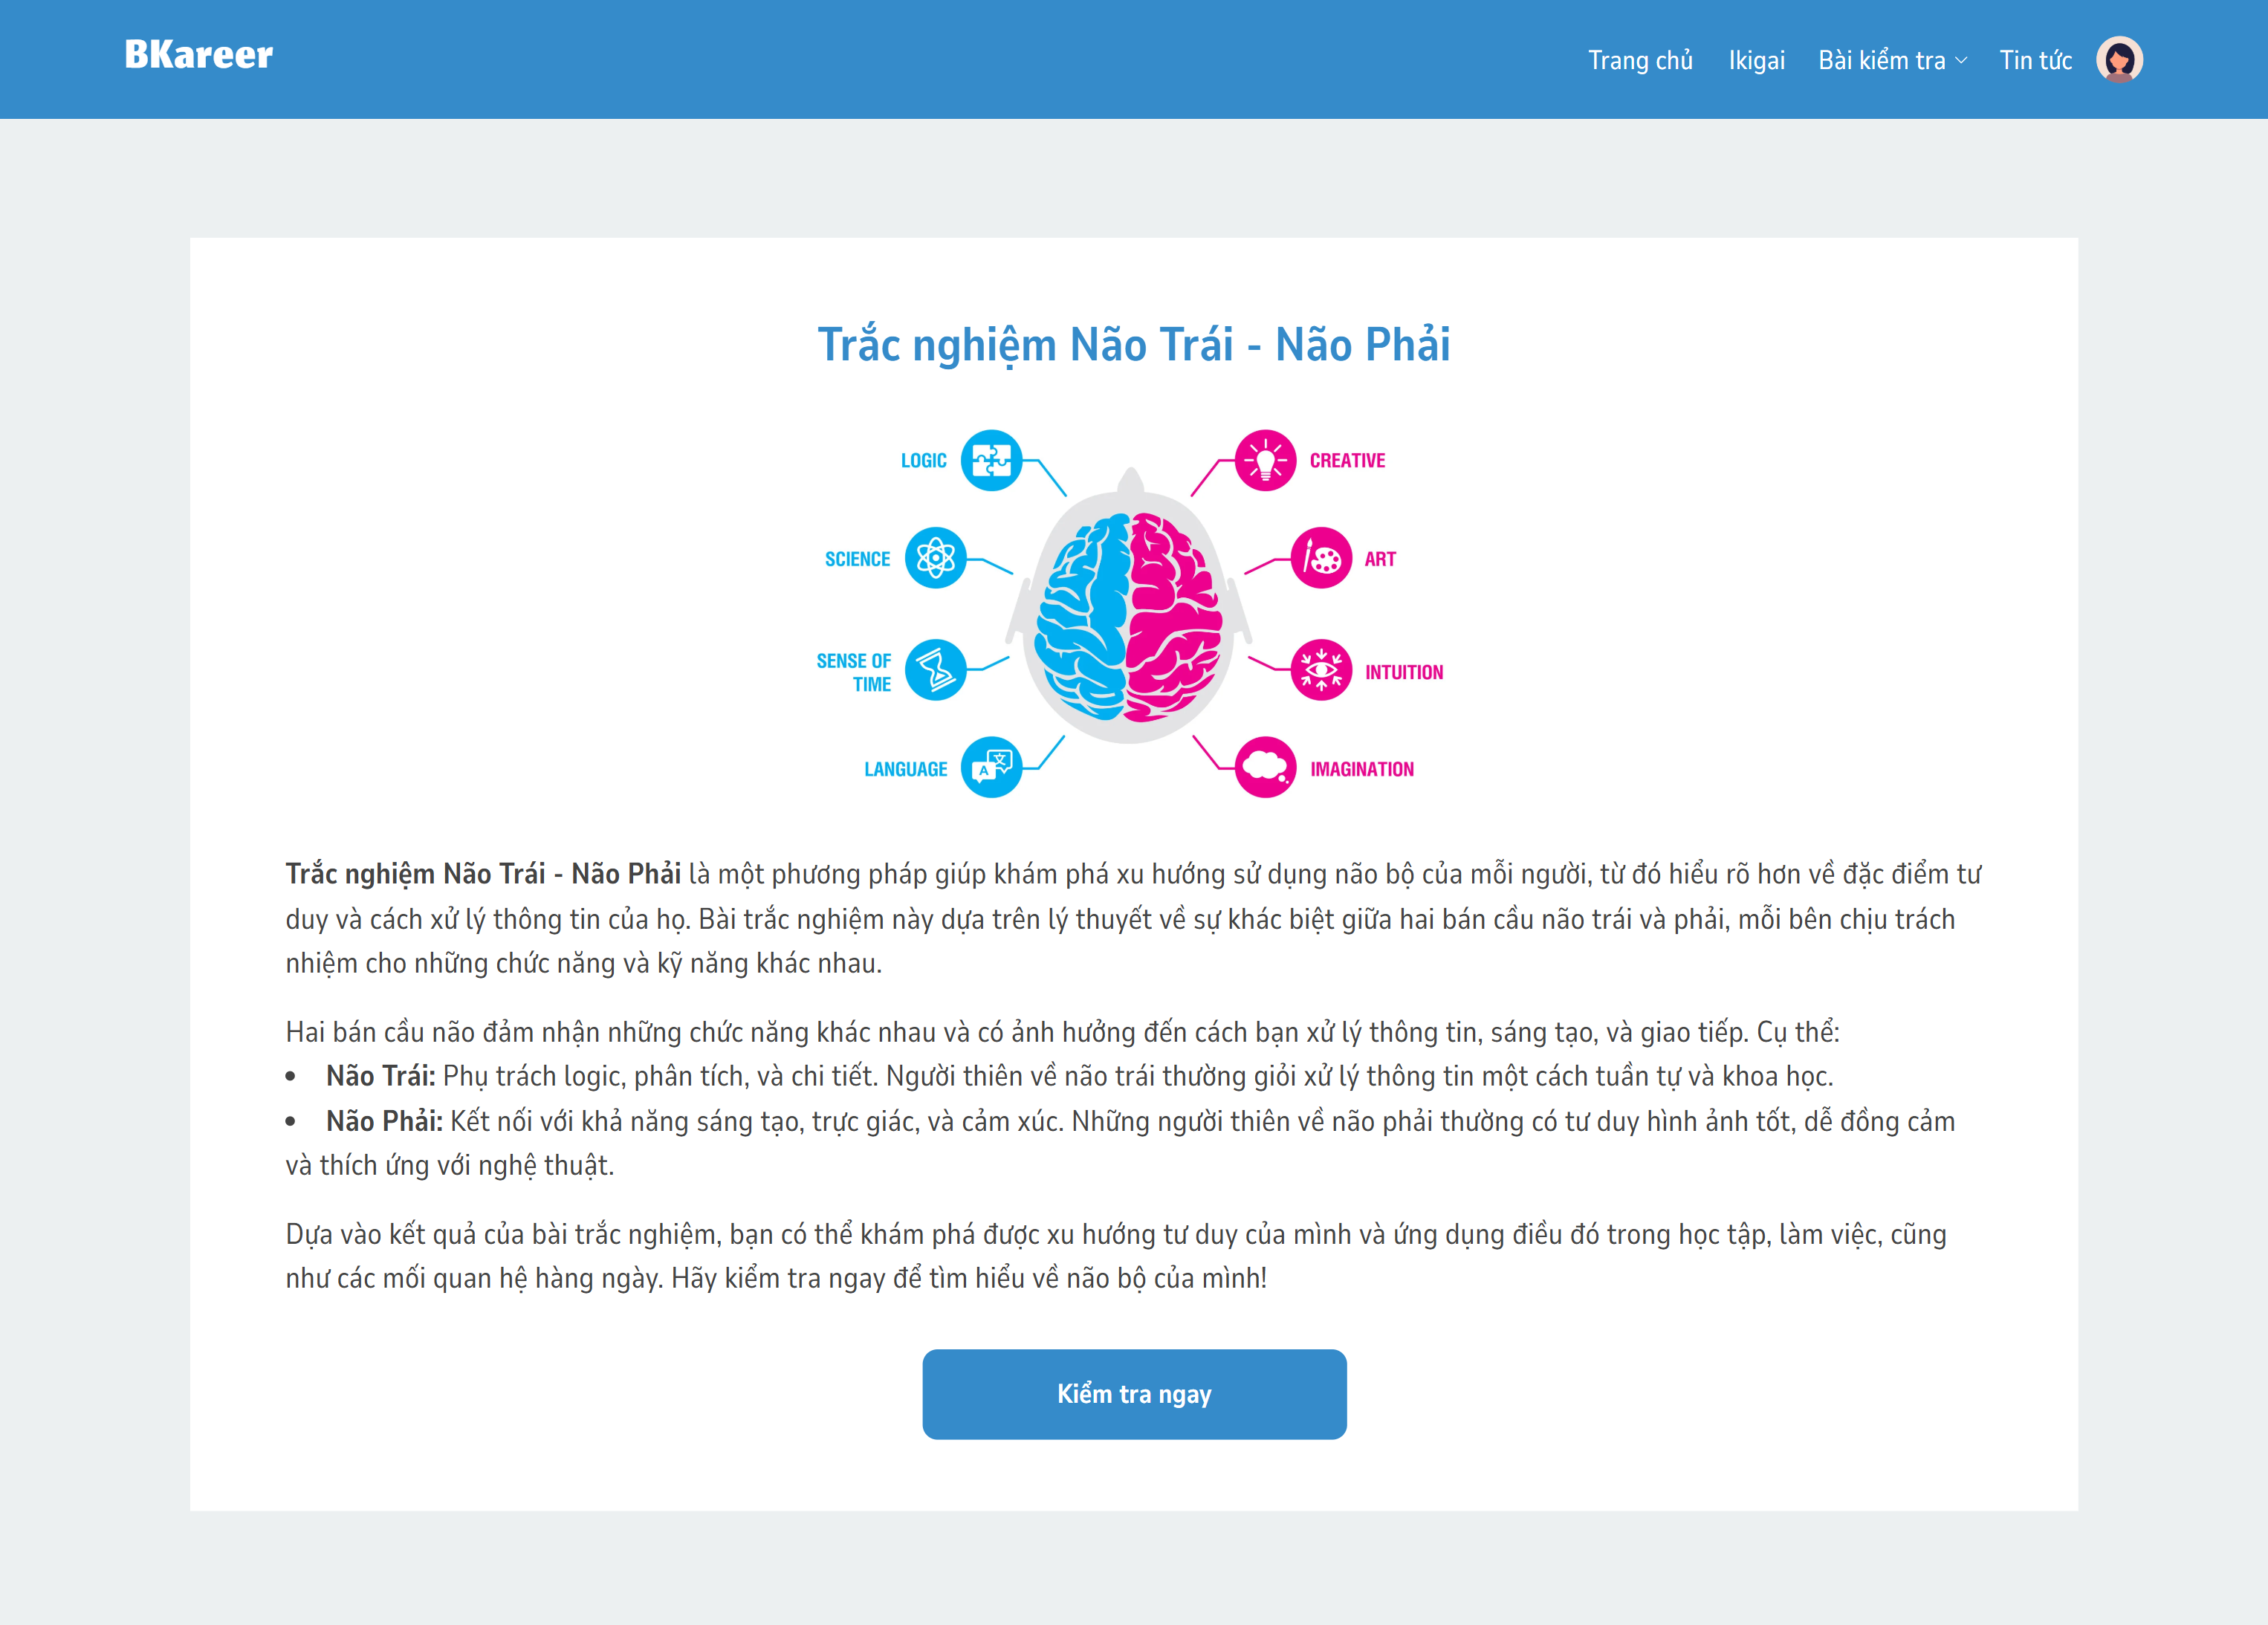
\includegraphics[width=0.8\textwidth]
    {images/chap5/lrBrainDetail.png}
    \vspace{0.5cm}
    \caption{Trang giới thiệu trắc nghiệm não trái - não phải}
\end{figure}

Các thành phần chính của trang giới thiệu trắc nghiệm não trái - não phải:
\begin{itemize}
    \item Hình ảnh minh họa: Hình ảnh minh họa cho nội dung của trang giúp người dùng có thể hình dung sơ lược về trang.
    \item Phần giới thiệu: Phần giới thiệu có vai trò cung cấp thông tin cần thiết cho người dùng, giúp người dùng hiểu rõ hơn về mục đích, nội dung và thành phần bài kiểm tra, từ đó có sự chuẩn bị tốt hơn.
    \item Nút:
        \begin{itemize}
            \item Nút ``Kiểm tra ngay": Cho phép người dùng chuyển đến trang kiểm tra để bắt đầu thực hiện bài kiểm tra ngay lập tức.
        \end{itemize}
\end{itemize}


%%%%%%%%%% Left Right Brain Test %%%%%%%%%%
\subsection{Trang thực hiện trắc nghiệm não trái - não phải}
Trang thực hiện trắc nghiệm não trái - não phải là một nền tảng trực tuyến được thiết kế để giúp người dùng xác định xem họ có xu hướng sử dụng não trái hay não phải nhiều hơn trong quá trình tư duy và xử lý thông tin.

Mục đích của trang thực hiện trắc nghiệm não trái - não phải:
\begin{itemize}
    \item Xác định ưu thế não: Giúp người dùng hiểu rõ hơn về cách thức tư duy của mình.
    \item Tìm hiểu về bản thân: Cung cấp thông tin về những đặc điểm tính cách, sở thích thường thấy ở người thuận não trái hoặc não phải.
    \item Tìm hiểu về phong cách học tập: Đưa ra gợi ý về phương pháp học tập phù hợp với mỗi kiểu não.
    \item Khám phá tiềm năng: Giúp người dùng nhận ra những điểm mạnh và điểm yếu của bản thân.
\end{itemize}

\begin{figure}[H]
    \centering
    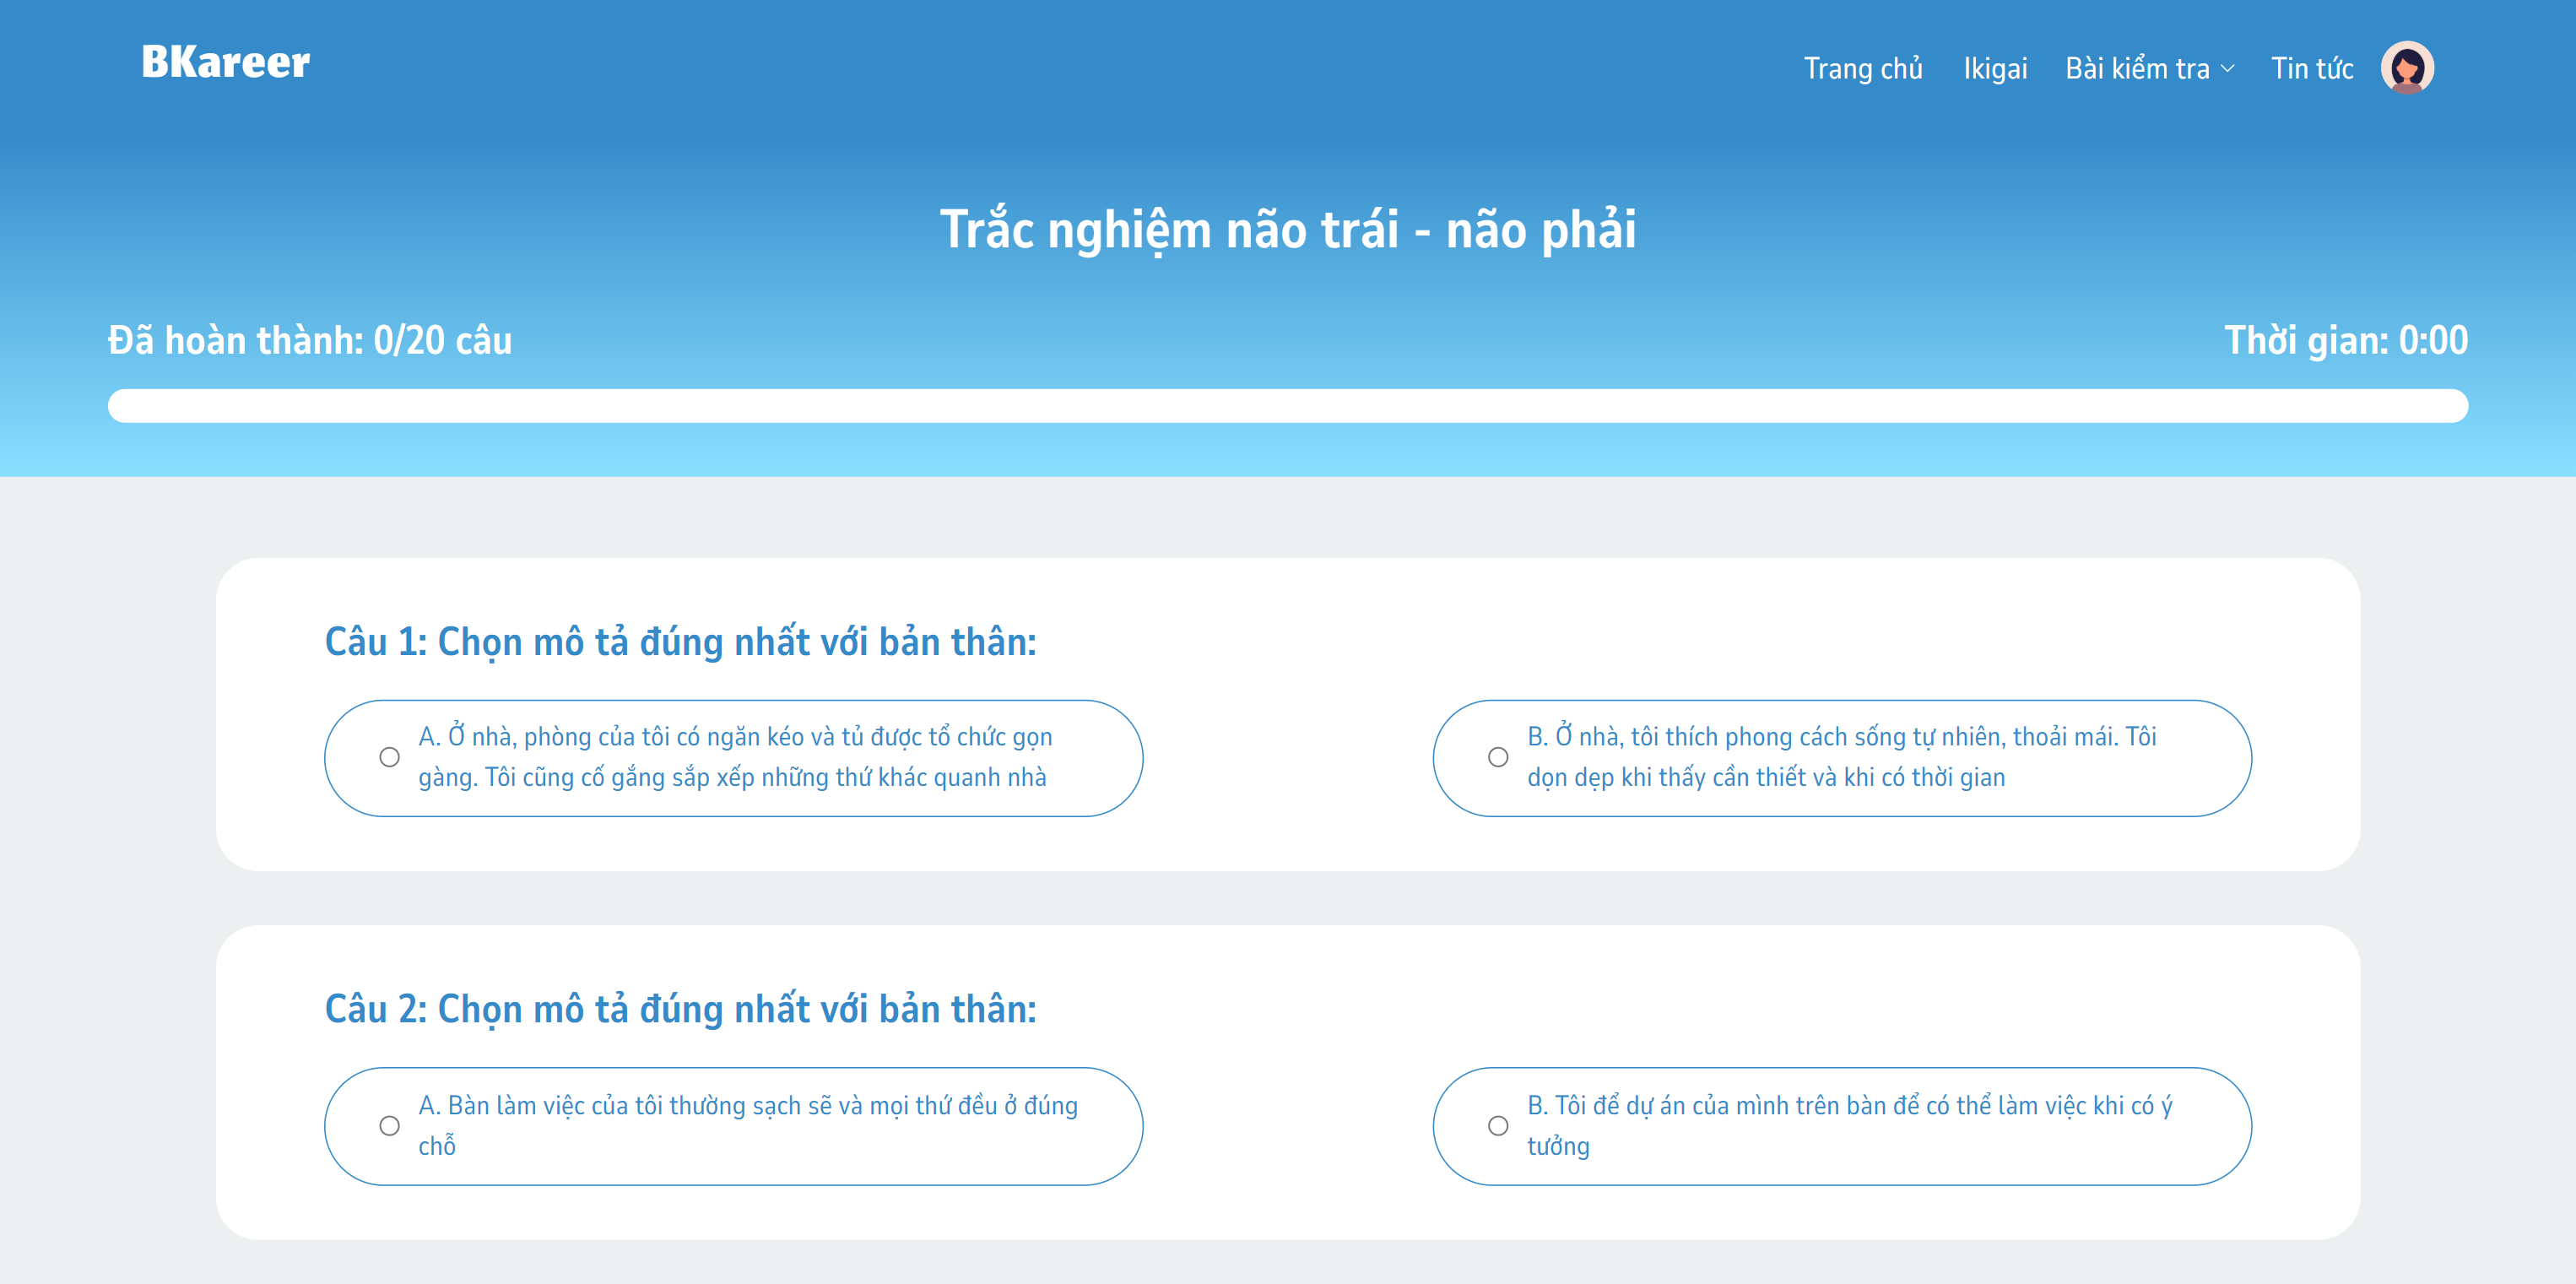
\includegraphics[width=0.8\textwidth]
    {images/chap5/lrBrain.png}
    \vspace{0.5cm}
    \caption{Trang thực hiện trắc nghiệm não trái - não phải}
\end{figure}

Các thành phần chính của trang thực hiện trắc nghiệm não trái - não phải:
\begin{itemize}
    \item Thanh tiến trình: Bao gồm tiến độ hoàn thành bài kiểm tra và đồng hồ đếm thời gian thực hiện bài kiểm tra.
    \item Các khối câu hỏi: Mỗi khối bao gồm 1 câu hỏi và 3 đáp án, cho phép người dùng chọn 1 trong 3 đáp án, và có thể thay đổi sau khi lựa chọn.
    \item Nút:
        \begin{itemize}
            \item Nút ``Xem kết quả": Hiển thị giao diện thông báo kết quả cho người dùng.
        \end{itemize}
\end{itemize}


%%%%%%%%%% Learning Style Detail %%%%%%%%%%
\subsection{Trang giới thiệu trắc nghiệm 3 thiên hướng học tập}
Trang giới thiệu trắc nghiệm 3 thiên hướng học tập là hoặc một phần của hệ thống cung cấp thông tin chi tiết về một công cụ đánh giá giúp người dùng xác định cách thức học tập hiệu quả nhất của bản thân. Trắc nghiệm này thường dựa trên lý thuyết về ba kiểu học tập chính: trực quan, thính giác và xúc giác.

Mục đích của trang giới thiệu trắc nghiệm 3 thiên hướng học tập:
\begin{itemize}
    \item Giải thích về 3 thiên hướng học tập: Trang web sẽ cung cấp định nghĩa rõ ràng về từng kiểu học tập, ví dụ minh họa và những đặc điểm nổi bật của người thuộc mỗi kiểu.
    \item Giới thiệu về trắc nghiệm: Giải thích cách thức hoạt động của trắc nghiệm, số câu hỏi và cách tính điểm.
    \item Cung cấp thông tin bổ sung: Có thể bao gồm các bài viết, tài liệu tham khảo liên quan đến các phương pháp học tập hiệu quả cho từng kiểu học tập.
\end{itemize}

\begin{figure}[H]
    \centering
    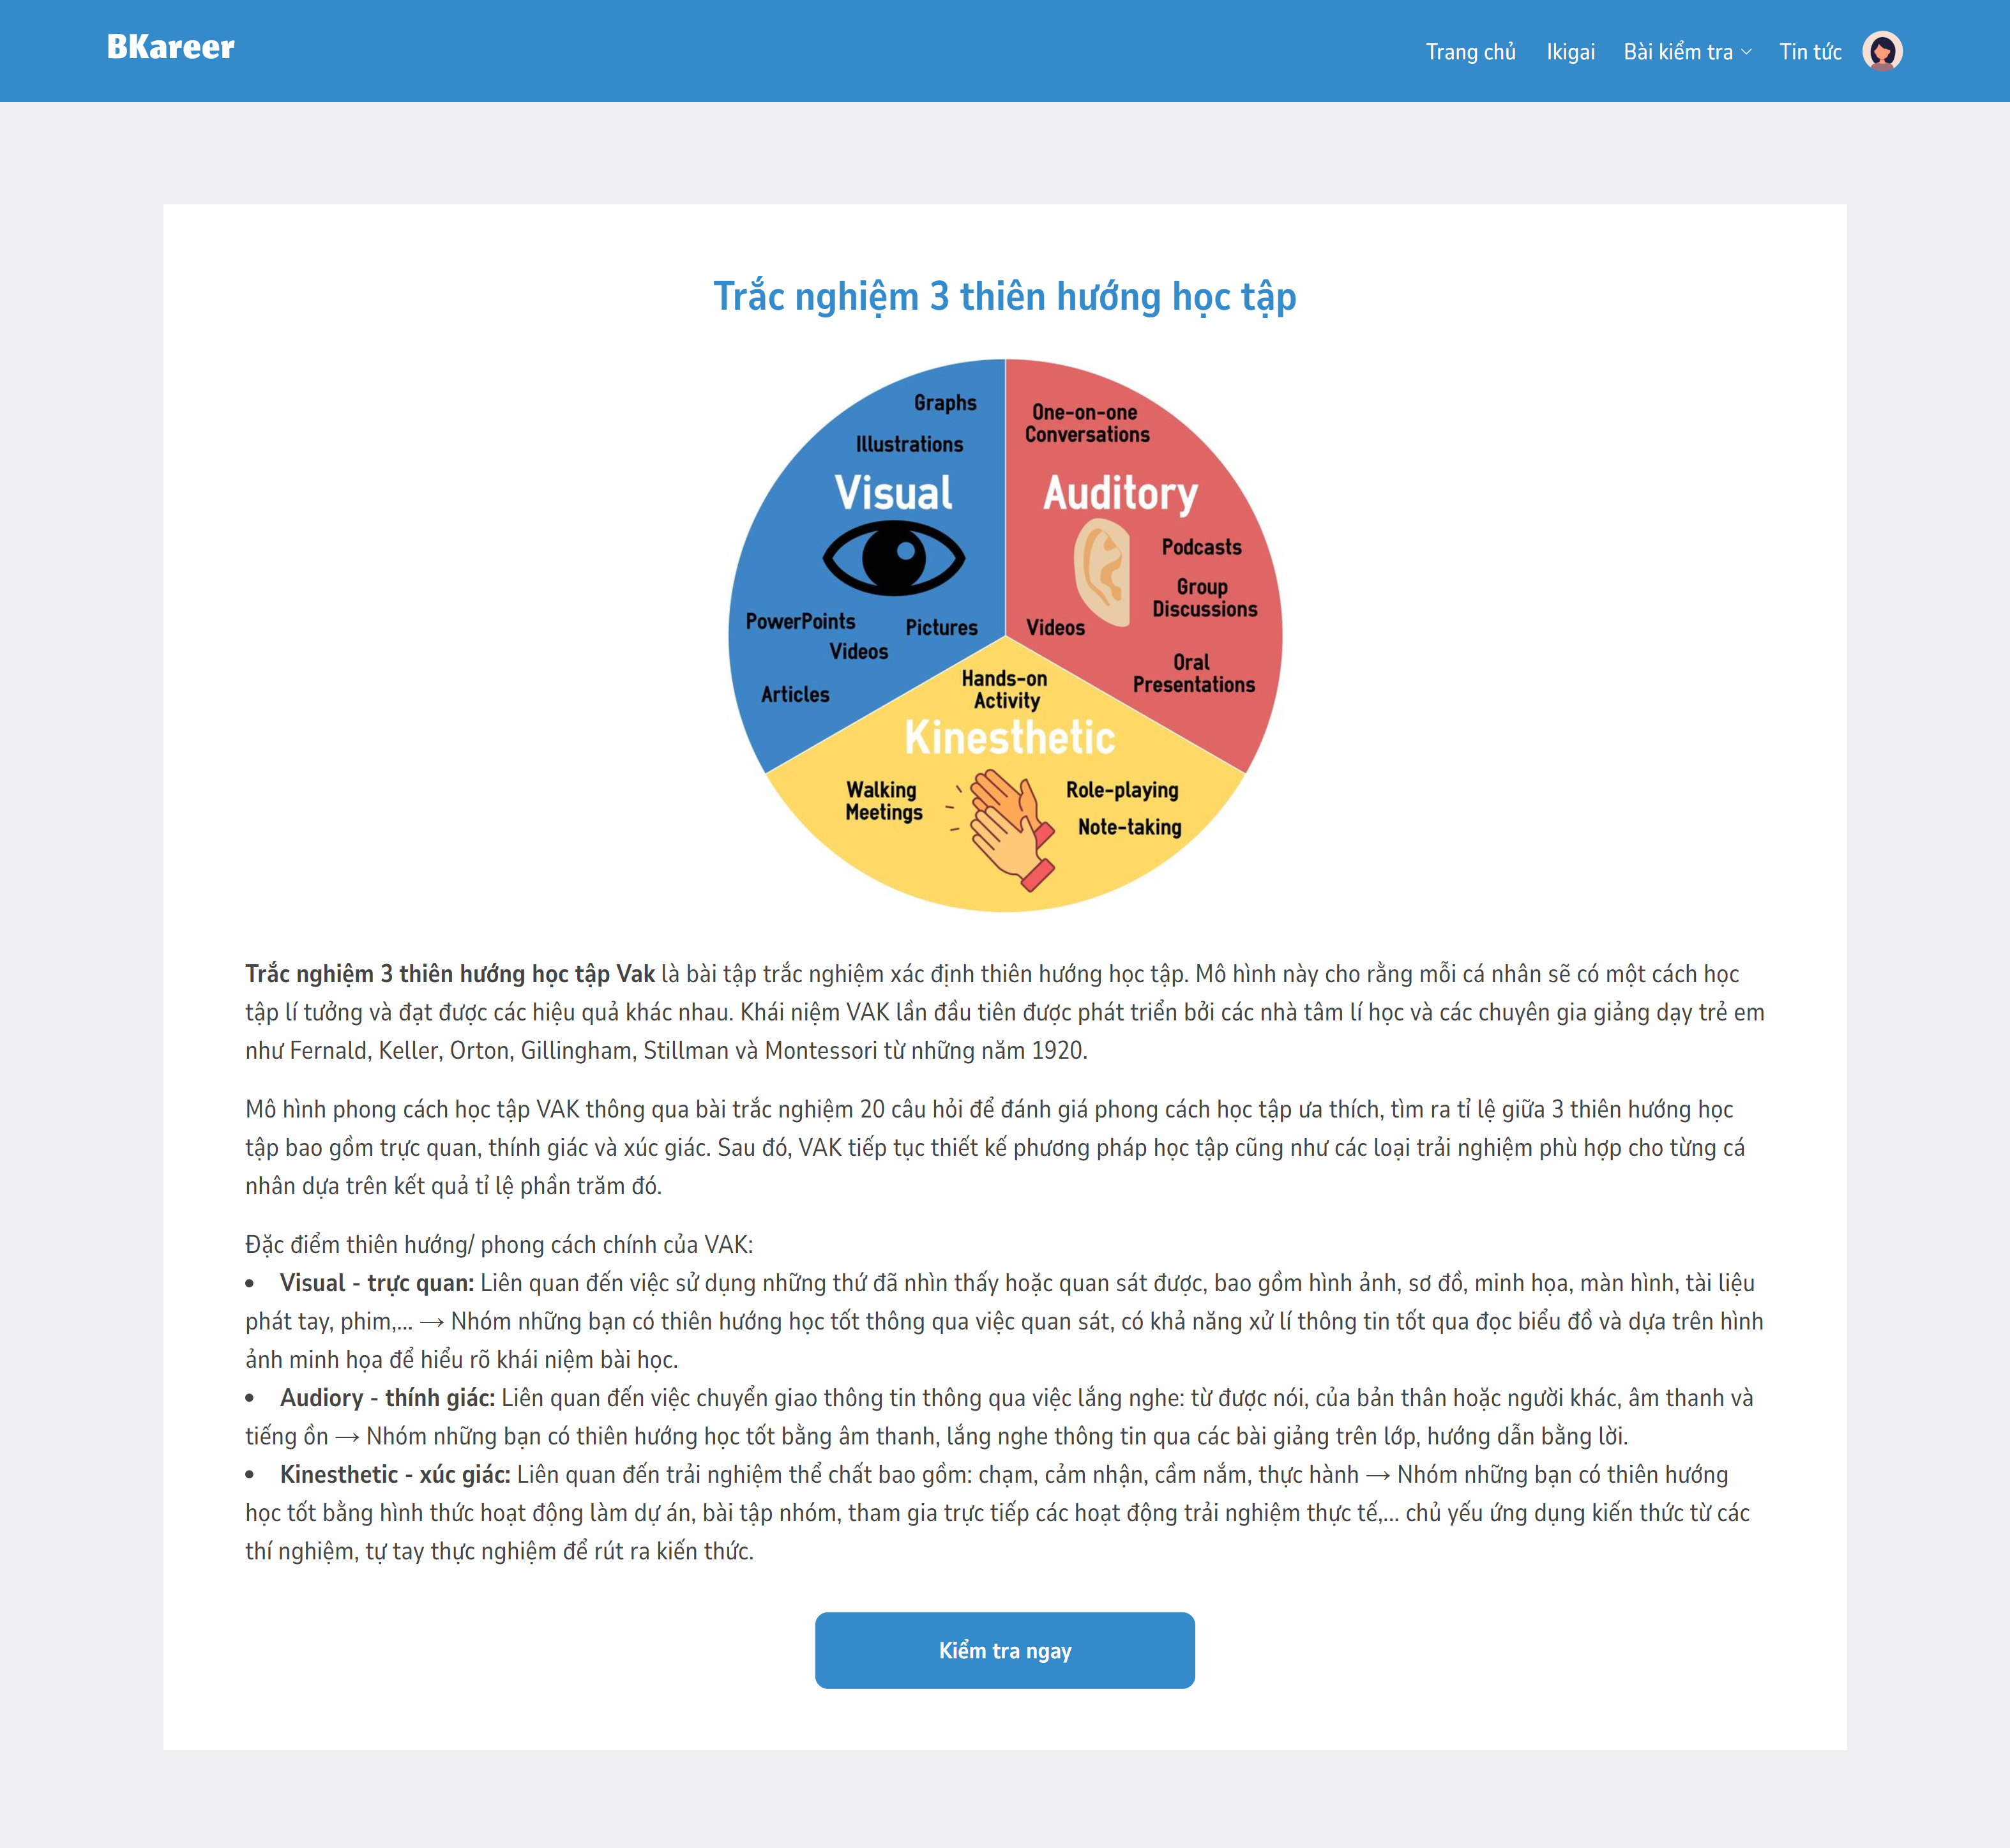
\includegraphics[width=0.8\textwidth]
    {images/chap5/learningStyleDetail.png}
    \vspace{0.5cm}
    \caption{Trang giới thiệu trắc nghiệm 3 thiên hướng học tập}
\end{figure}

Các thành phần chính của trang giới thiệu trắc nghiệm 3 thiên hướng học tập:
\begin{itemize}
    \item Hình ảnh minh họa: Hình ảnh minh họa cho nội dung của trang giúp người dùng có thể hình dung sơ lược về trang.
    \item Phần giới thiệu: Phần giới thiệu có vai trò cung cấp thông tin cần thiết cho người dùng, giúp người dùng hiểu rõ hơn về mục đích, nội dung và thành phần bài kiểm tra, từ đó có sự chuẩn bị tốt hơn.
    \item Nút:
        \begin{itemize}
            \item Nút ``Kiểm tra ngay": Cho phép người dùng chuyển đến trang kiểm tra để bắt đầu thực hiện bài kiểm tra ngay lập tức.
        \end{itemize}
\end{itemize}


%%%%%%%%%% Learning Style Test %%%%%%%%%%
\subsection{Trang thực hiện trắc nghiệm 3 thiên hướng học tập}
Trang thực hiện trắc nghiệm 3 thiên hướng học tập là một giao diện được thiết kế để người dùng có thể tương tác trực tiếp với bài trắc nghiệm, nhằm xác định phong cách học tập chủ yếu của bản thân. Đây là một công cụ hữu ích giúp mỗi người hiểu rõ hơn về cách thức học tập hiệu quả nhất, từ đó cải thiện kết quả học tập và tăng cường sự tự tin.

Mục đích của trang thực hiện trắc nghiệm 3 thiên hướng học tập:
\begin{itemize}
    \item Xác định phong cách học tập: Giúp người dùng nhận biết được mình thuộc kiểu học tập trực quan, thính giác hay xúc giác.
    \item Tùy chỉnh phương pháp học tập: Cung cấp những gợi ý cụ thể về cách học tập phù hợp với từng kiểu, giúp người dùng tối ưu hóa quá trình học tập của mình.
    \item Nâng cao hiệu quả học tập: Giúp người học đạt được kết quả cao hơn trong học tập bằng cách tận dụng tối đa điểm mạnh và khắc phục điểm yếu của bản thân.
    \item Tăng cường sự tự tin: Khi hiểu rõ về cách học của mình, người học sẽ cảm thấy tự tin hơn và chủ động hơn trong quá trình học tập.
    \item Cung cấp thông tin hữu ích: Cung cấp thêm các kiến thức về các phương pháp học tập hiệu quả, các công cụ hỗ trợ học tập, giúp người dùng có thêm nhiều lựa chọn để cải thiện quá trình học tập của mình.
\end{itemize}

\begin{figure}[H]
    \centering
    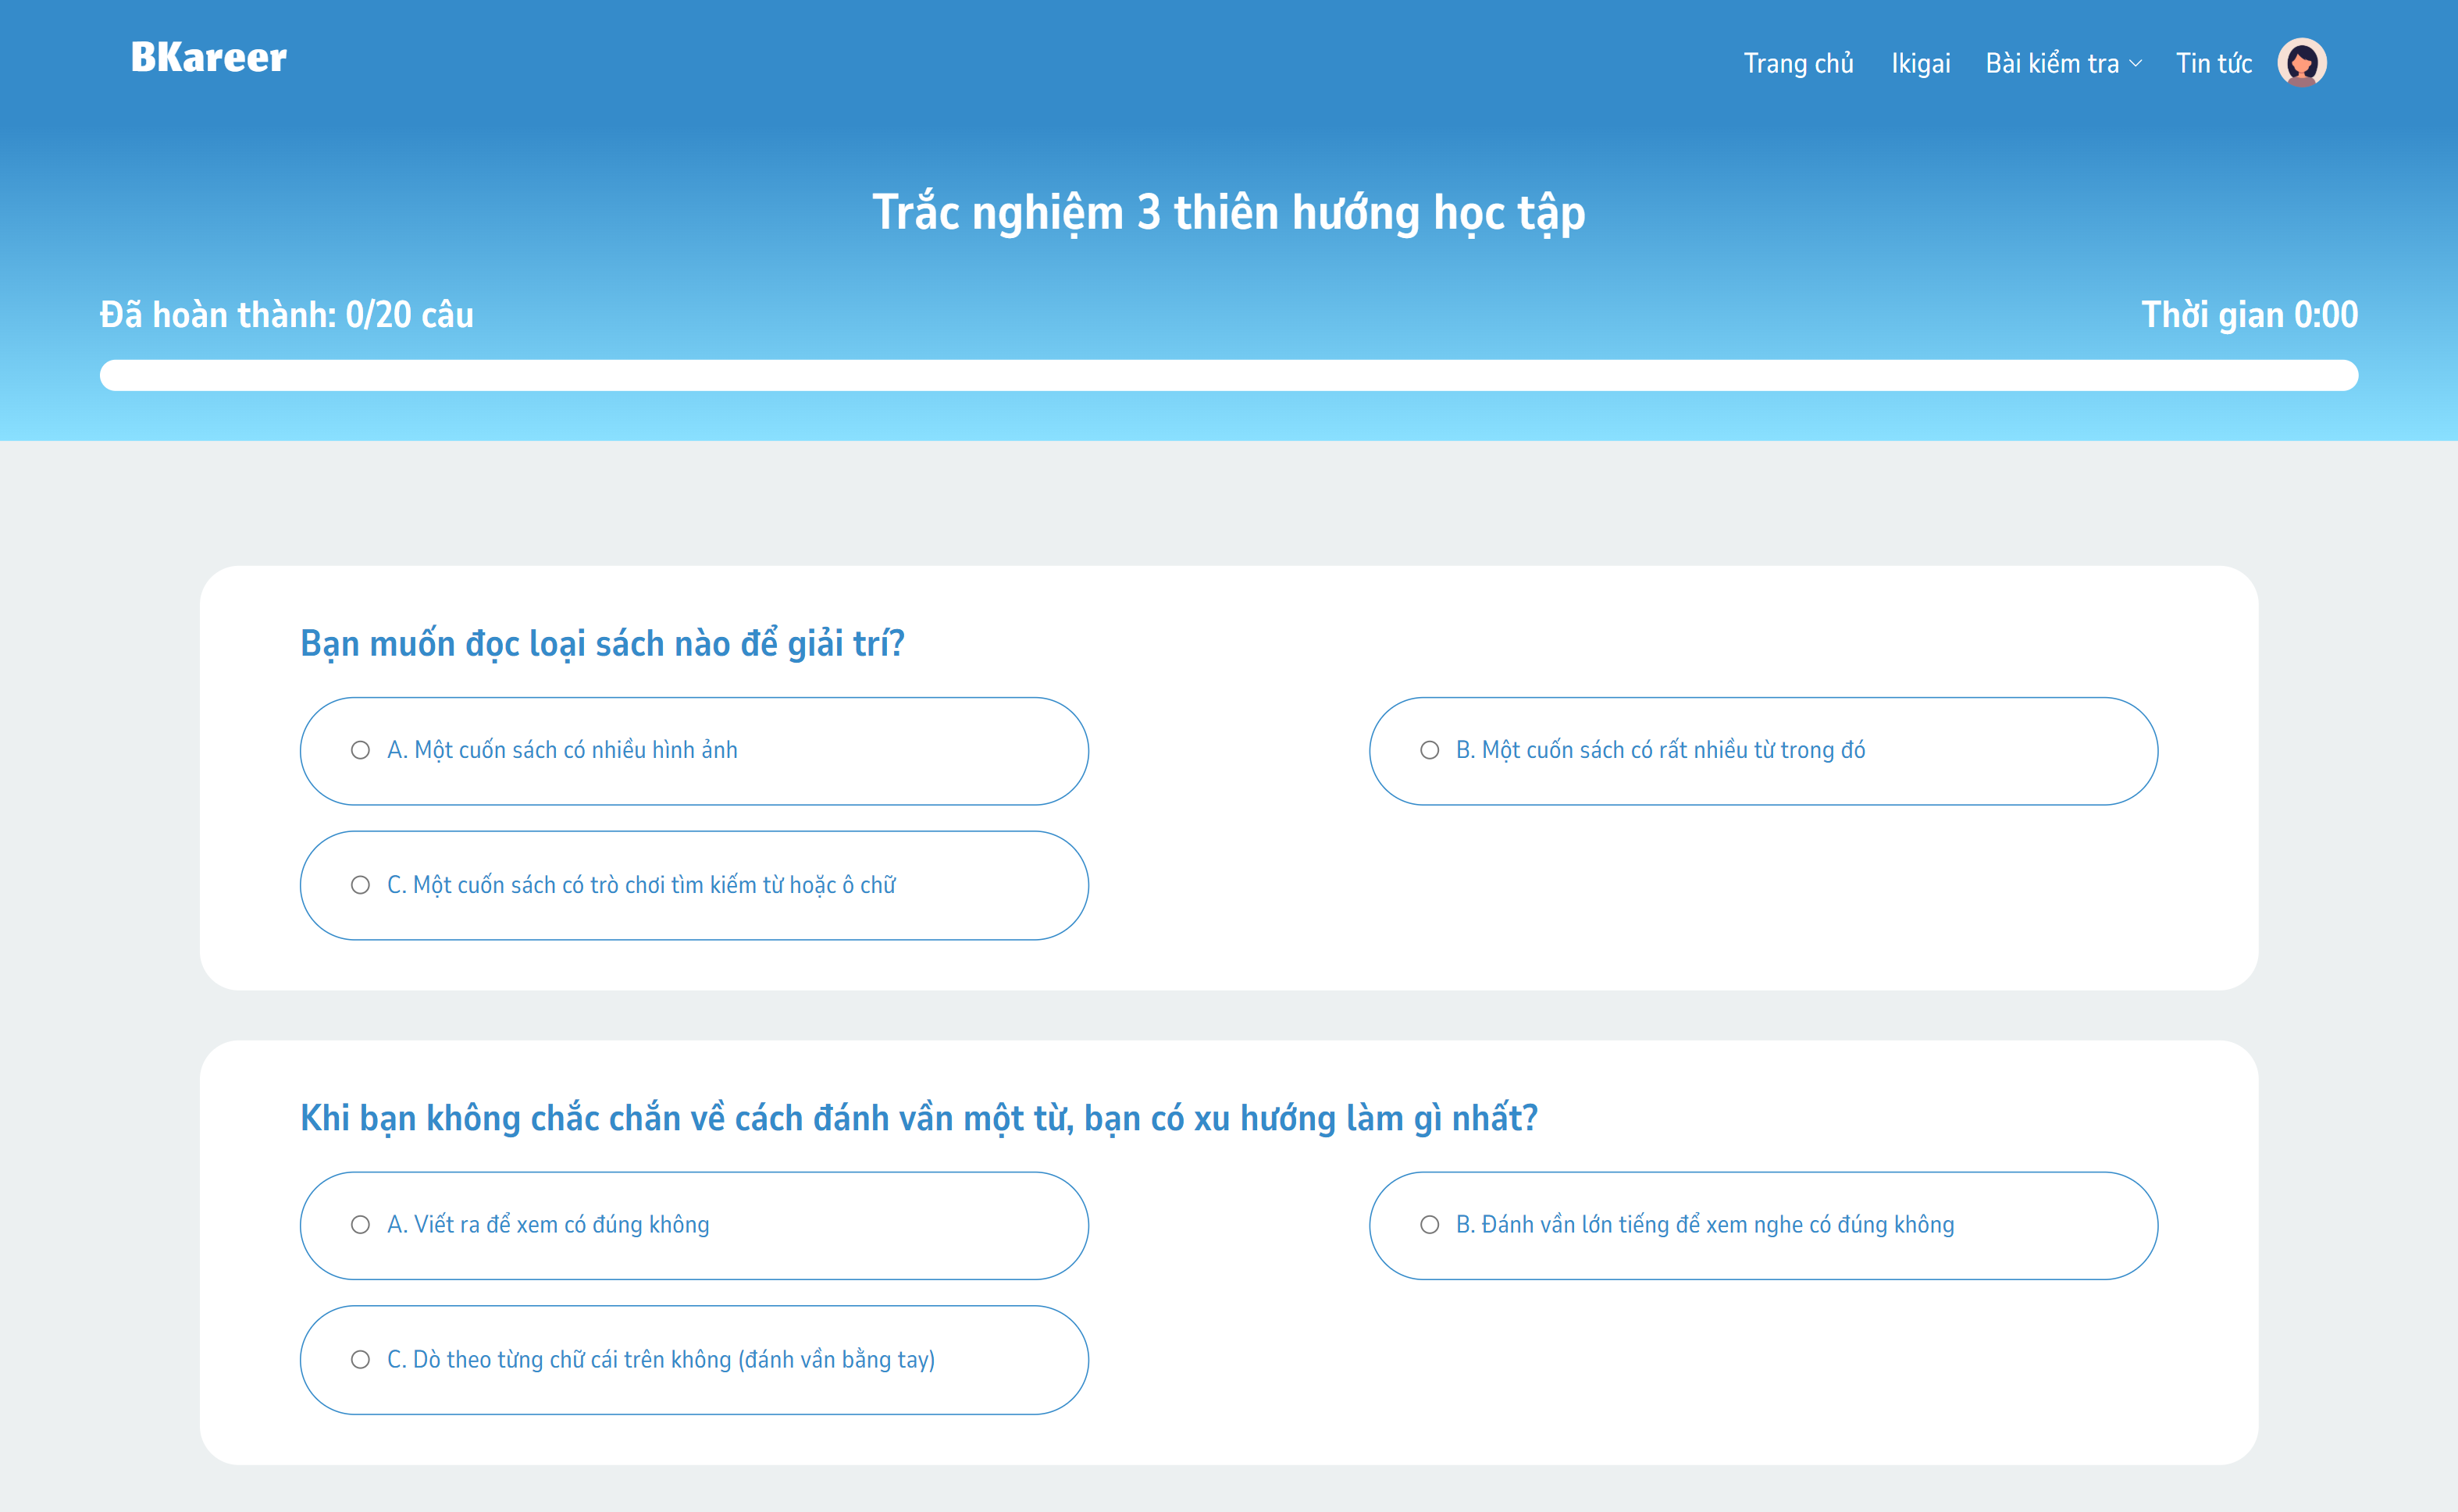
\includegraphics[width=0.8\textwidth]
    {images/chap5/learningStyle.png}
    \vspace{0.5cm}
    \caption{Trang thực hiện trắc nghiệm 3 thiên hướng học tập}
\end{figure}

Các thành phần chính của trang thực hiện trắc nghiệm 3 thiên hướng học tập:
\begin{itemize}
    \item Thanh tiến trình: Bao gồm tiến độ hoàn thành bài kiểm tra và đồng hồ đếm thời gian thực hiện bài kiểm tra.
    \item Các khối câu hỏi: Mỗi khối bao gồm 1 câu hỏi và 3 đáp án, cho phép người dùng chọn 1 trong 3 đáp án, và có thể thay đổi sau khi lựa chọn.
    \item Nút:
        \begin{itemize}
            \item Nút ``Xem kết quả": Hiển thị giao diện thông báo kết quả cho người dùng.
        \end{itemize}
\end{itemize}


%%%%%%%%%% Big Five Detail %%%%%%%%%%
\subsection{Trang giới thiệu trắc nghiệm 5 yếu tố tính cách}
Trang giới thiệu trắc nghiệm 5 yếu tố tính cách là một trang web hoặc một phần của một trang web, cung cấp thông tin chi tiết về một công cụ đánh giá giúp người dùng hiểu rõ hơn về tính cách của bản thân dựa trên mô hình 5 yếu tố tính cách (Big Five).

Mục đích của trang giới thiệu trắc nghiệm 5 yếu tố tính cách:
\begin{itemize}
    \item Giải thích về mô hình 5 yếu tố: Trang web sẽ cung cấp định nghĩa rõ ràng về từng yếu tố tính cách (Hướng ngoại, Dễ chịu, Cởi mở, Tận tâm và Nhạy cảm), tầm quan trọng của việc hiểu rõ tính cách.
    \item Giới thiệu về trắc nghiệm: Giải thích cách thức hoạt động của trắc nghiệm, loại câu hỏi và cách tính điểm.
    \item Nêu rõ lợi ích của việc xác định 5 yếu tố tính cách: Giúp người dùng hiểu rõ hơn về điểm mạnh, điểm yếu, sở thích, phù hợp với công việc nào, nên học ngành gì,...
\end{itemize}

\begin{figure}[H]
    \centering
    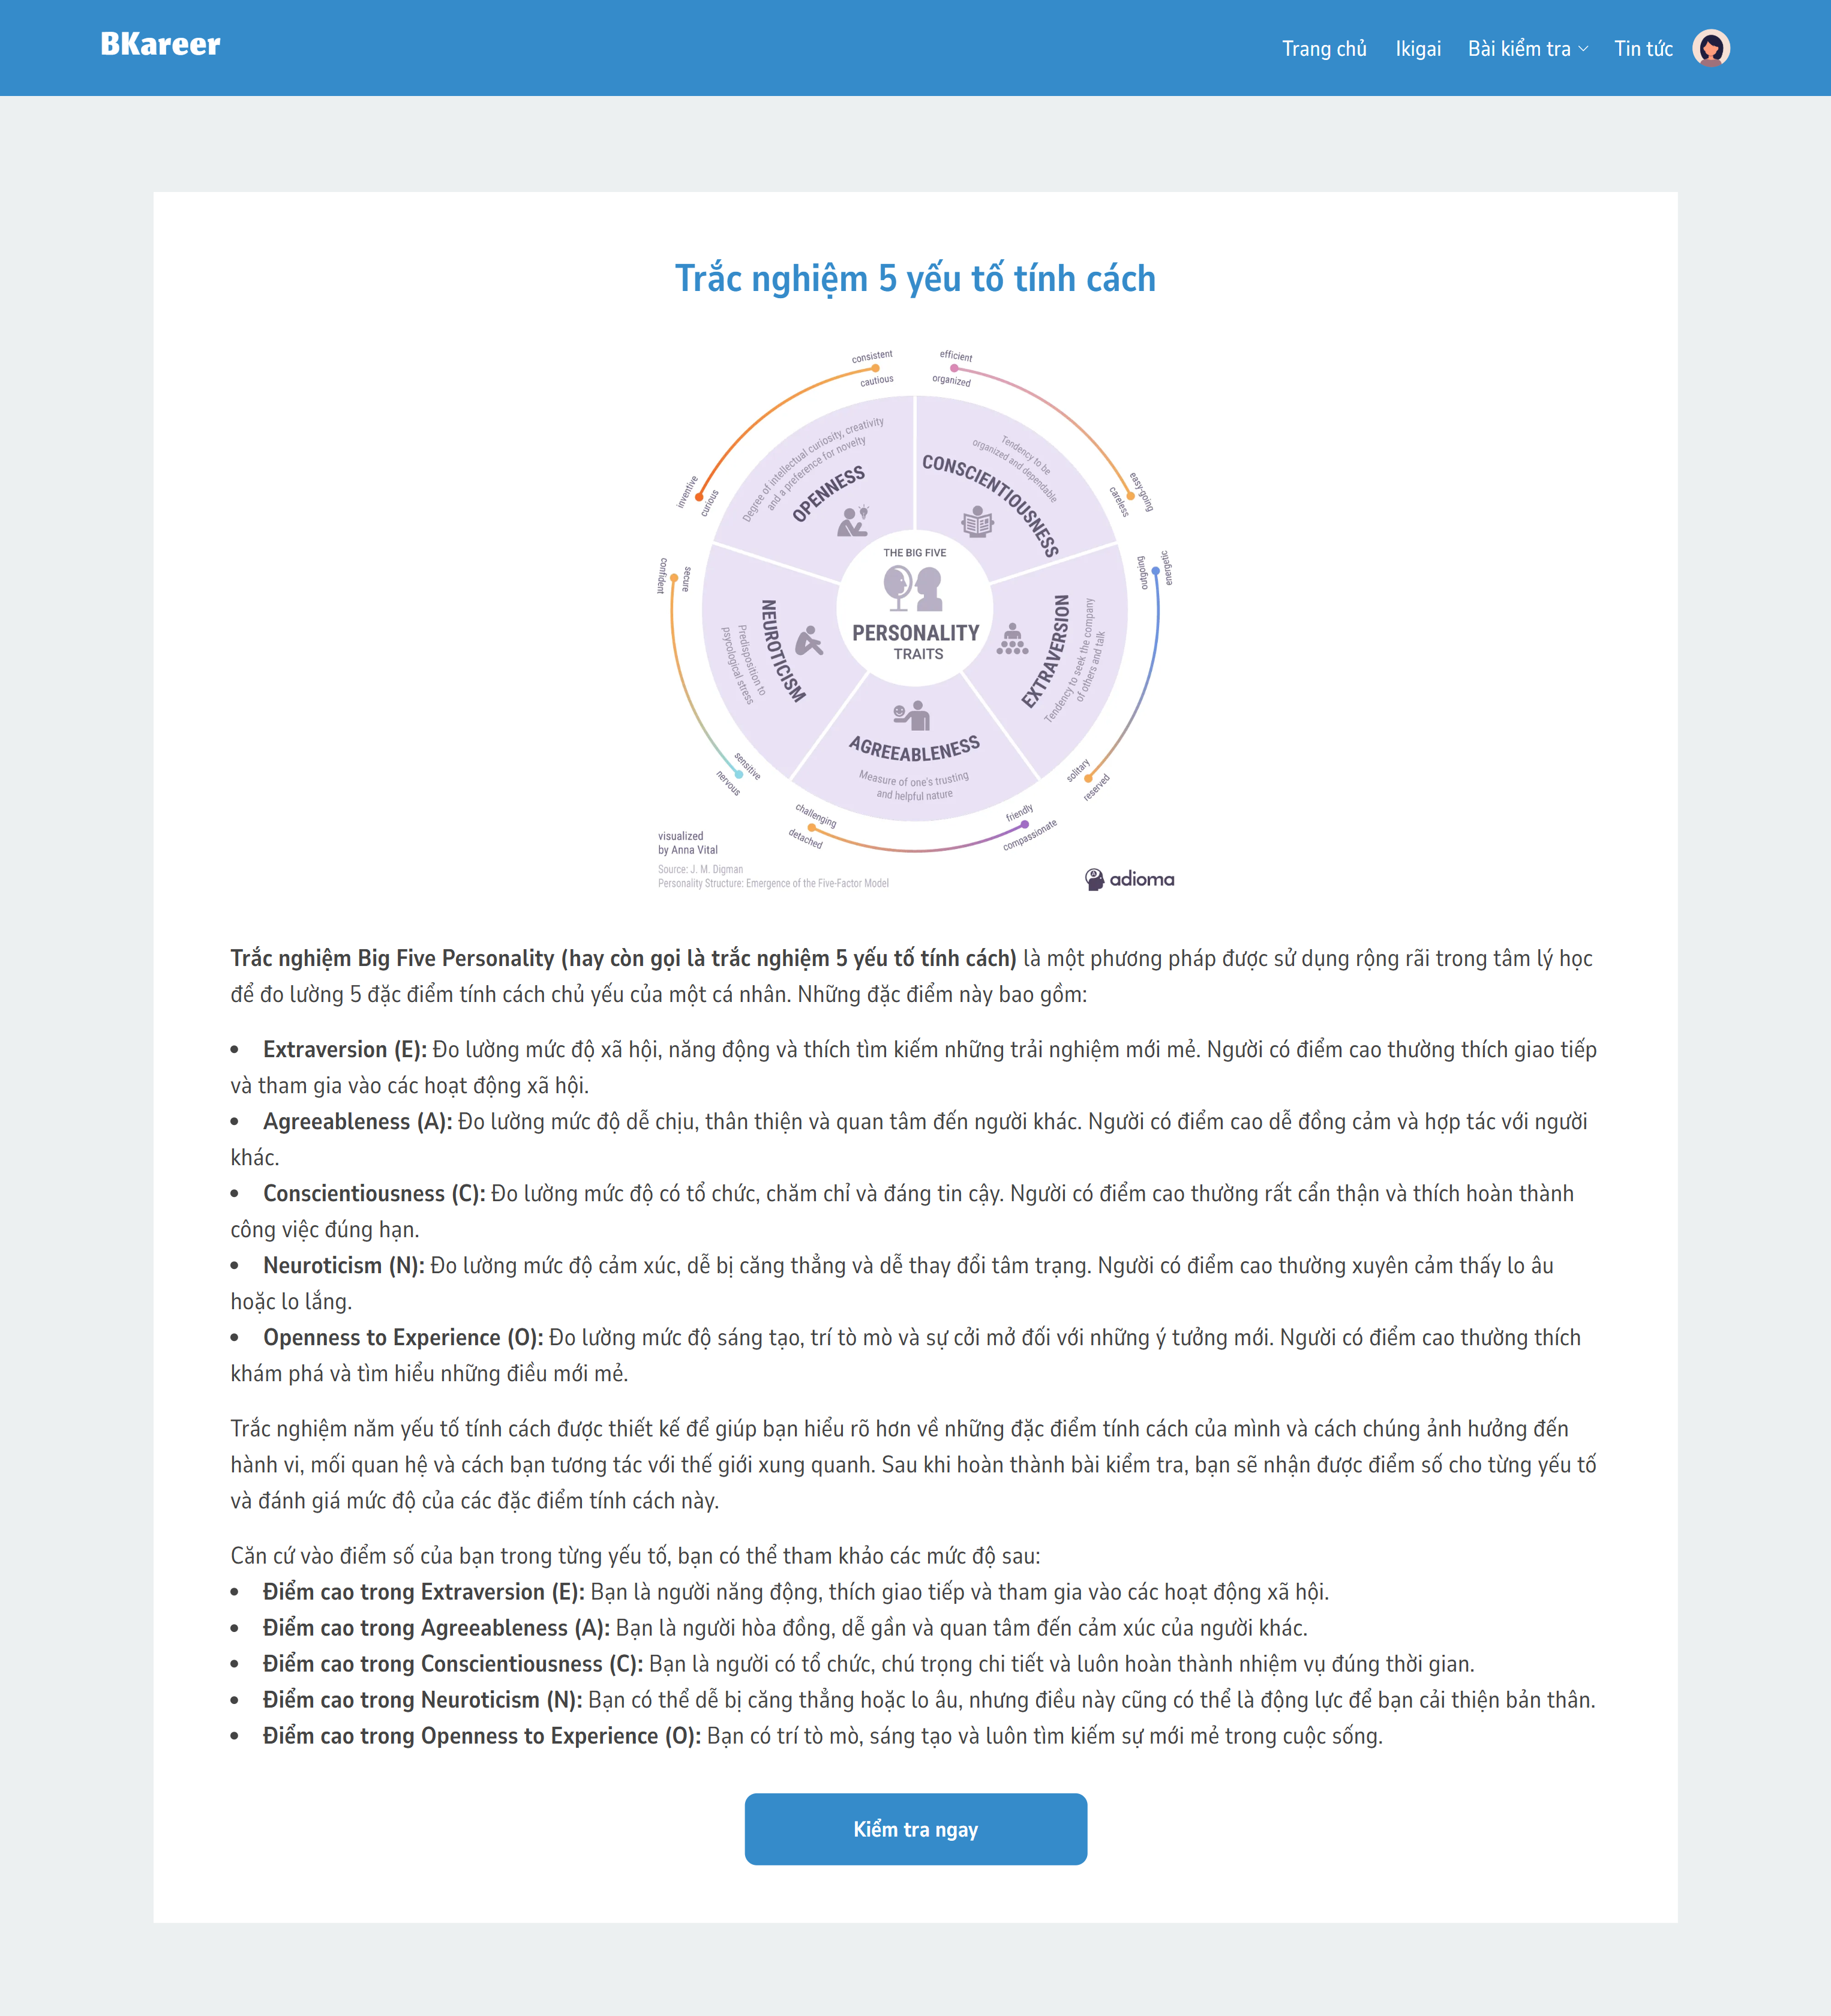
\includegraphics[width=0.8\textwidth]
    {images/chap5/fivePerDetail.png}
    \vspace{0.5cm}
    \caption{Trang giới thiệu trắc nghiệm 5 yếu tố tính cách}
\end{figure}

Các thành phần chính của trang giới thiệu trắc nghiệm 5 yếu tố tính cách:
\begin{itemize}
    \item Hình ảnh minh họa: Hình ảnh minh họa cho nội dung của trang giúp người dùng có thể hình dung sơ lược về trang.
    \item Phần giới thiệu: Phần giới thiệu có vai trò cung cấp thông tin cần thiết cho người dùng, giúp người dùng hiểu rõ hơn về mục đích, nội dung và thành phần bài kiểm tra, từ đó có sự chuẩn bị tốt hơn.
    \item Nút:
        \begin{itemize}
            \item Nút ``Kiểm tra ngay": Cho phép người dùng chuyển đến trang kiểm tra để bắt đầu thực hiện bài kiểm tra ngay lập tức.
        \end{itemize}
\end{itemize}


%%%%%%%%%% Big Five Test %%%%%%%%%%
\subsection{Trang thực hiện trắc nghiệm 5 yếu tố tính cách}
Trang thực hiện trắc nghiệm 5 yếu tố tính cách là một nền tảng trực tuyến được thiết kế để giúp người dùng khám phá và hiểu rõ hơn về tính cách của bản thân dựa trên mô hình Big Five. Mô hình này chia tính cách của con người thành 5 yếu tố chính:
\begin{itemize}
    \item Cởi mở: Đề cập đến sự tò mò, sáng tạo, yêu thích trải nghiệm mới.
    \item Tận tâm: Liên quan đến tính kỷ luật, trách nhiệm, và sự kiên trì.
    \item Hướng ngoại: Chỉ ra mức độ yêu thích giao tiếp, sự sôi nổi và năng lượng.
    \item Dễ chịu: Liên quan đến sự hợp tác, độ tin cậy và sự quan tâm đến người khác.
    \item Nhạy cảm: Mô tả mức độ lo lắng, căng thẳng và sự thay đổi cảm xúc.
\end{itemize}

Mục đích của trang thực hiện trắc nghiệm 5 yếu tố tính cách:
\begin{itemize}
    \item Đánh giá tính cách: Giúp người dùng hiểu rõ hơn về bản thân mình.
    \item Tìm hiểu về bản thân: Cung cấp thông tin về điểm mạnh, điểm yếu, sở thích và xu hướng hành vi.
    \item Ứng dụng trong cuộc sống: Giúp người dùng lựa chọn nghề nghiệp phù hợp, cải thiện các mối quan hệ và phát triển bản thân.
    \item Đưa ra gợi ý: Cung cấp những lời khuyên về cách phát huy điểm mạnh, khắc phục điểm yếu và ứng dụng kết quả trắc nghiệm vào cuộc sống.
\end{itemize}

\begin{figure}[H]
    \centering
    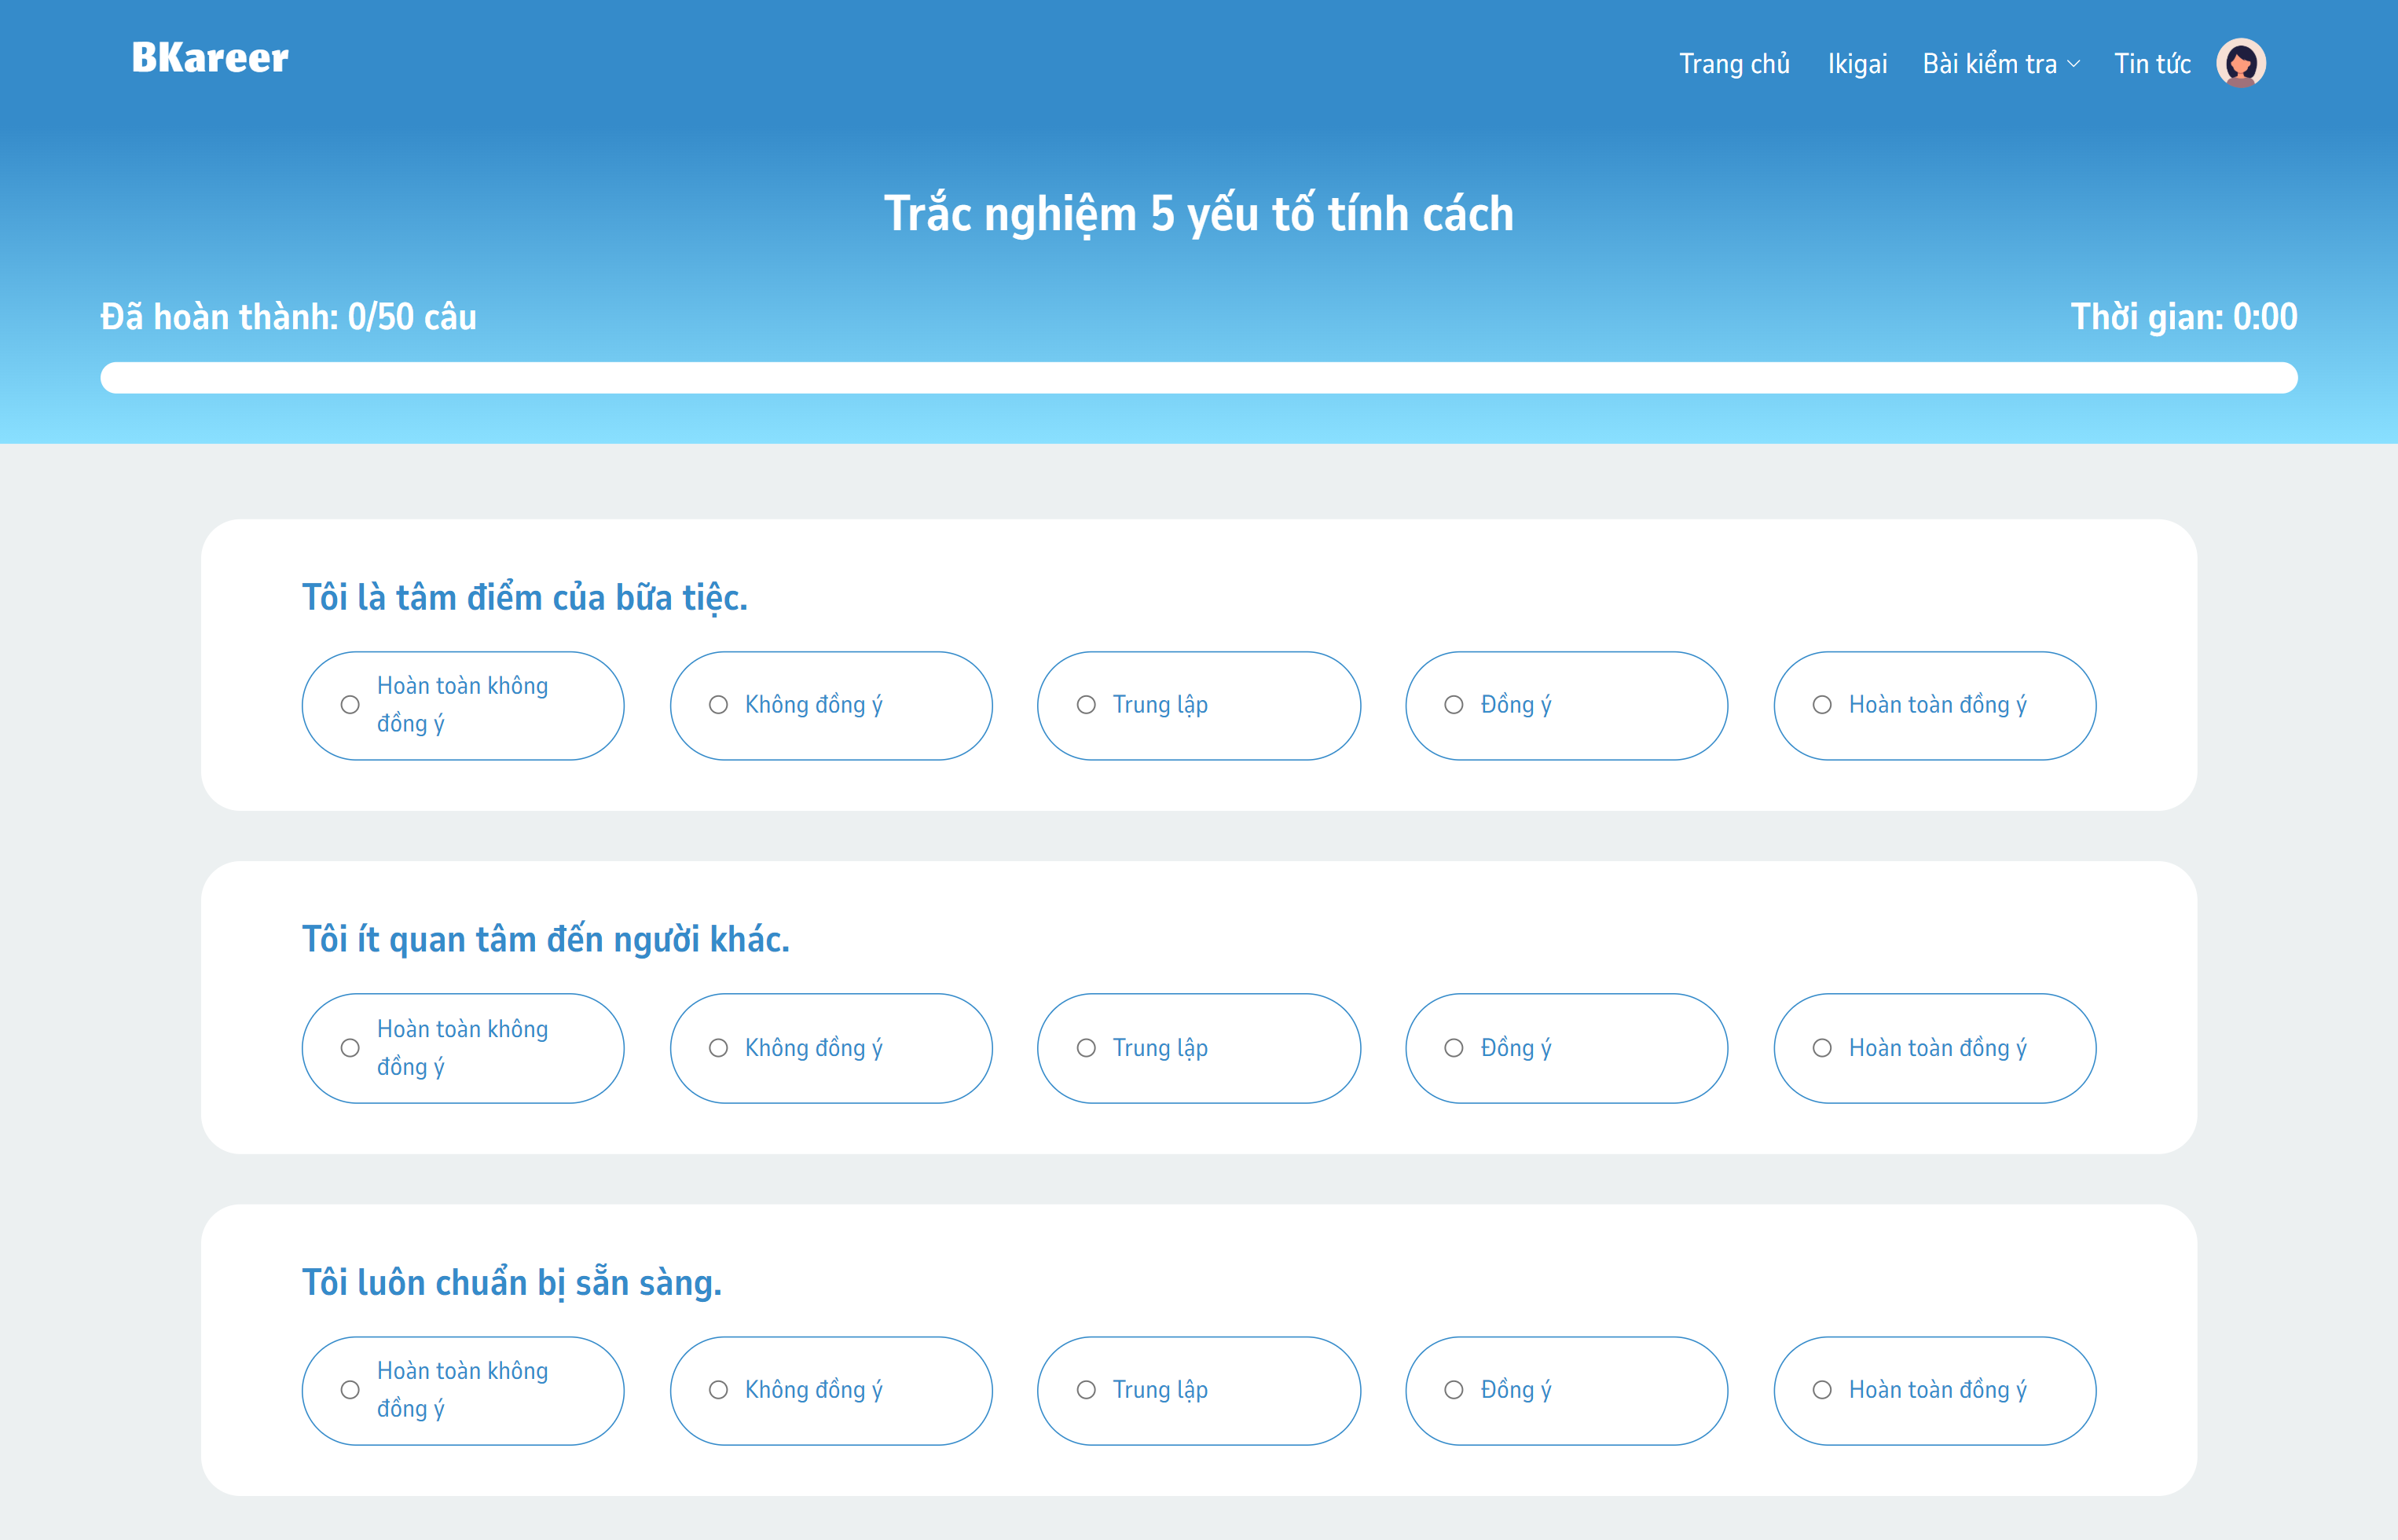
\includegraphics[width=0.8\textwidth]
    {images/chap5/fivePer.png}
    \vspace{0.5cm}
    \caption{Trang thực hiện trắc nghiệm 5 yếu tố tính cách}
\end{figure}

Các thành phần chính của trang thực hiện trắc nghiệm 5 yếu tố tính cách:
\begin{itemize}
    \item Thanh tiến trình: Bao gồm tiến độ hoàn thành bài kiểm tra và đồng hồ đếm thời gian thực hiện bài kiểm tra.
    \item Các khối câu hỏi: Mỗi khối bao gồm 1 câu hỏi và 5 đáp án theo mức độ từ hoàn toàn không đồng ý đến hoàn toàn đồng ý, cho phép người dùng chọn 1 trong 5 đáp án, và có thể thay đổi sau khi lựa chọn.
    \item Nút:
        \begin{itemize}
            \item Nút ``Xem kết quả": Hiển thị giao diện thông báo kết quả cho người dùng.
        \end{itemize}
\end{itemize}


%%%%%%%%%% Work Style Detail %%%%%%%%%%
\subsection{Trang giới thiệu trắc nghiệm phong cách làm việc}
Trang giới thiệu trắc nghiệm phong cách làm việc là một nền tảng trực tuyến cung cấp thông tin chi tiết về một công cụ đánh giá giúp người dùng hiểu rõ hơn về cách thức làm việc của mình. Thông qua việc làm bài trắc nghiệm, người dùng có thể xác định được phong cách làm việc chủ đạo của mình, từ đó khám phá ra điểm mạnh, điểm yếu, cũng như tìm ra cách làm việc hiệu quả nhất.

Mục đích của trang giới thiệu trắc nghiệm phong cách làm việc:
\begin{itemize}
    \item Giải thích về phong cách làm việc: Trang web sẽ cung cấp định nghĩa rõ ràng về các phong cách làm việc phổ biến.
    \item Giới thiệu về trắc nghiệm: Giải thích cách thức hoạt động của trắc nghiệm, loại câu hỏi và cách tính điểm.
    \item Nêu rõ lợi ích của việc xác định phong cách làm việc: Giúp người dùng:
        \begin{itemize}
            \item Tìm được công việc phù hợp
            \item Xây dựng mối quan hệ tốt đẹp với đồng nghiệp
            \item Nâng cao hiệu quả làm việc
            \item Phát triển bản thân
        \end{itemize}
\end{itemize}

\begin{figure}[H]
    \centering
    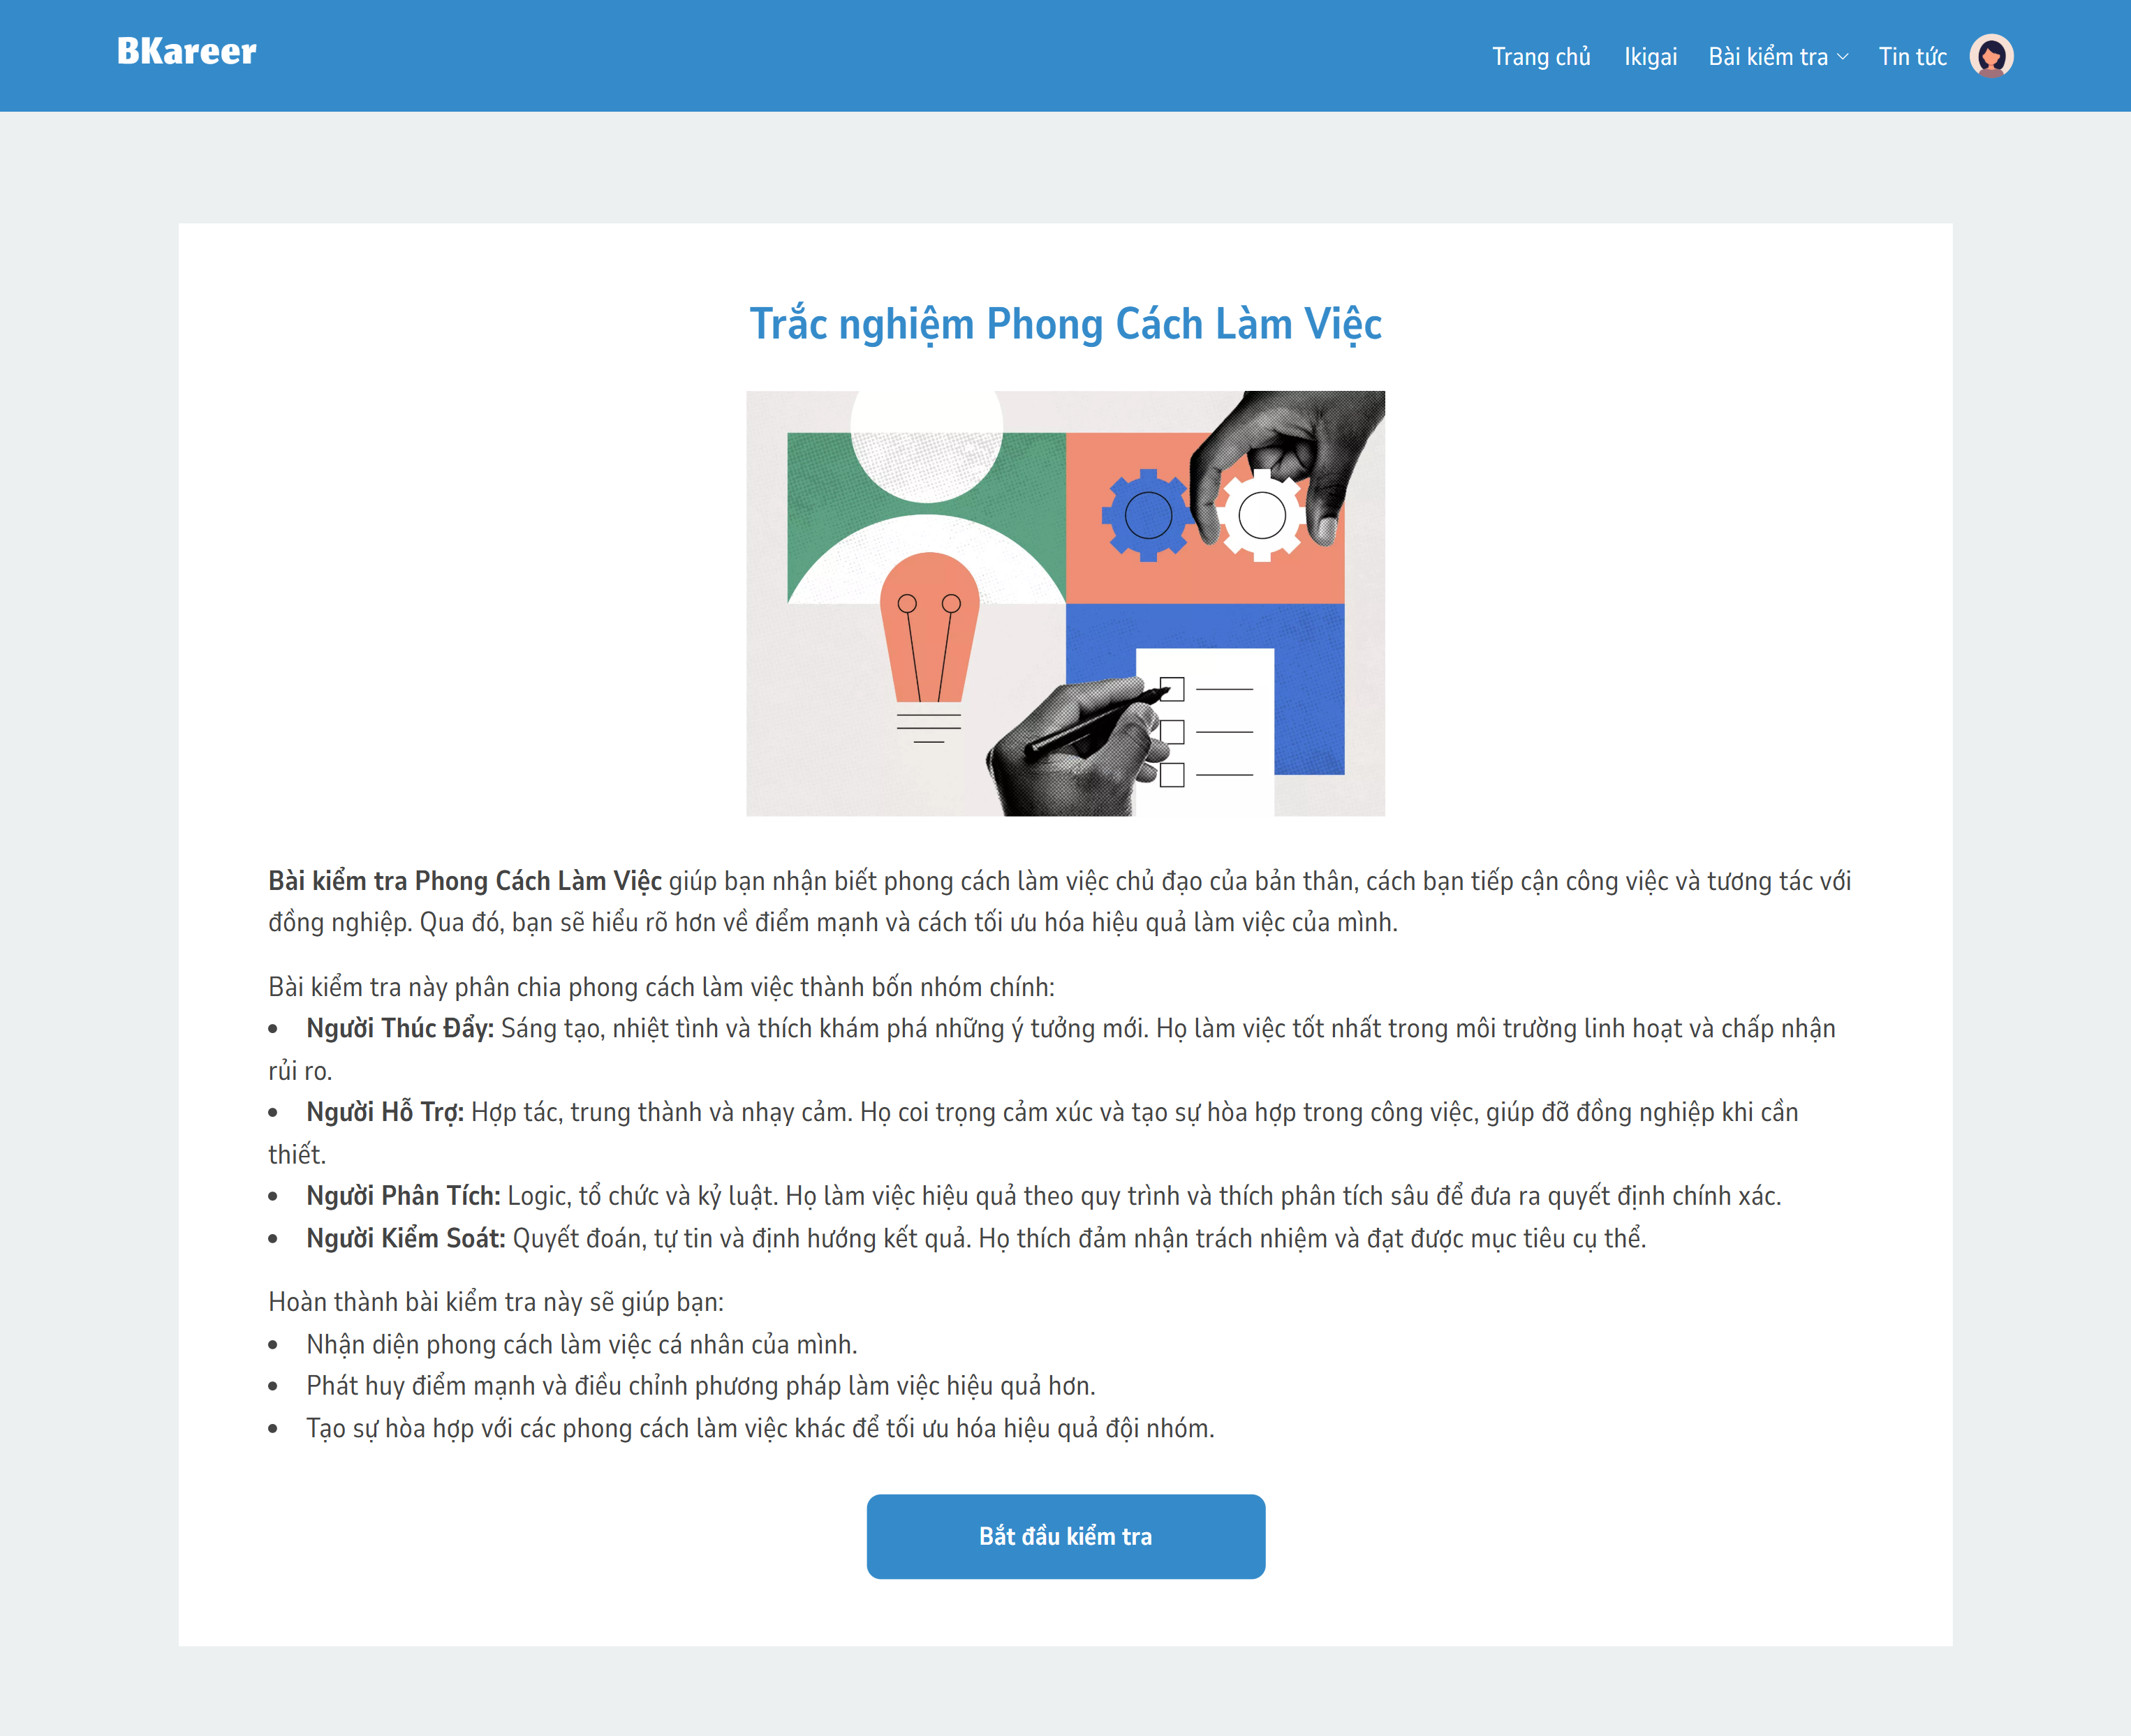
\includegraphics[width=0.8\textwidth]
    {images/chap5/workStyleDetail.png}
    \vspace{0.5cm}
    \caption{Trang giới thiệu trắc nghiệm phong cách làm việc}
\end{figure}

Các thành phần chính của trang giới thiệu trắc nghiệm phong cách làm việc:
\begin{itemize}
    \item Hình ảnh minh họa: Hình ảnh minh họa cho nội dung của trang giúp người dùng có thể hình dung sơ lược về trang.
    \item Phần giới thiệu: Phần giới thiệu có vai trò cung cấp thông tin cần thiết cho người dùng, giúp người dùng hiểu rõ hơn về mục đích, nội dung và thành phần bài kiểm tra, từ đó có sự chuẩn bị tốt hơn.
    \item Nút:
        \begin{itemize}
            \item Nút ``Kiểm tra ngay": Cho phép người dùng chuyển đến trang kiểm tra để bắt đầu thực hiện bài kiểm tra ngay lập tức.
        \end{itemize}
\end{itemize}


%%%%%%%%%% Work Style Test %%%%%%%%%%
\subsection{Trang thực hiện trắc nghiệm phong cách làm việc}
Trang thực hiện trắc nghiệm phong cách làm việc là một nền tảng trực tuyến giúp người dùng đánh giá và hiểu rõ hơn về cách thức làm việc của bản thân. Thông qua các câu hỏi và các lựa chọn mô tả từng phong cách làm việc, trắc nghiệm sẽ giúp bạn xác định được những đặc điểm về hành vi, thái độ và cách tiếp cận công việc thường thấy ở bạn.

Mục đích của trang thực hiện trắc nghiệm phong cách làm việc:
\begin{itemize}
    \item Hiểu rõ bản thân: Giúp bạn nhận biết điểm mạnh, điểm yếu, sở thích và phong cách làm việc phù hợp với bản thân.
    \item Lựa chọn nghề nghiệp: Đưa ra gợi ý về những ngành nghề, vị trí công việc phù hợp với phong cách làm việc của bạn.
    \item Cải thiện hiệu suất làm việc: Đưa ra những lời khuyên để bạn phát huy tối đa điểm mạnh và khắc phục điểm yếu trong công việc.
    \item Xây dựng mối quan hệ đồng nghiệp: Giúp bạn hiểu rõ hơn về cách làm việc của người khác và xây dựng mối quan hệ tốt đẹp hơn.
\end{itemize}

\begin{figure}[H]
    \centering
    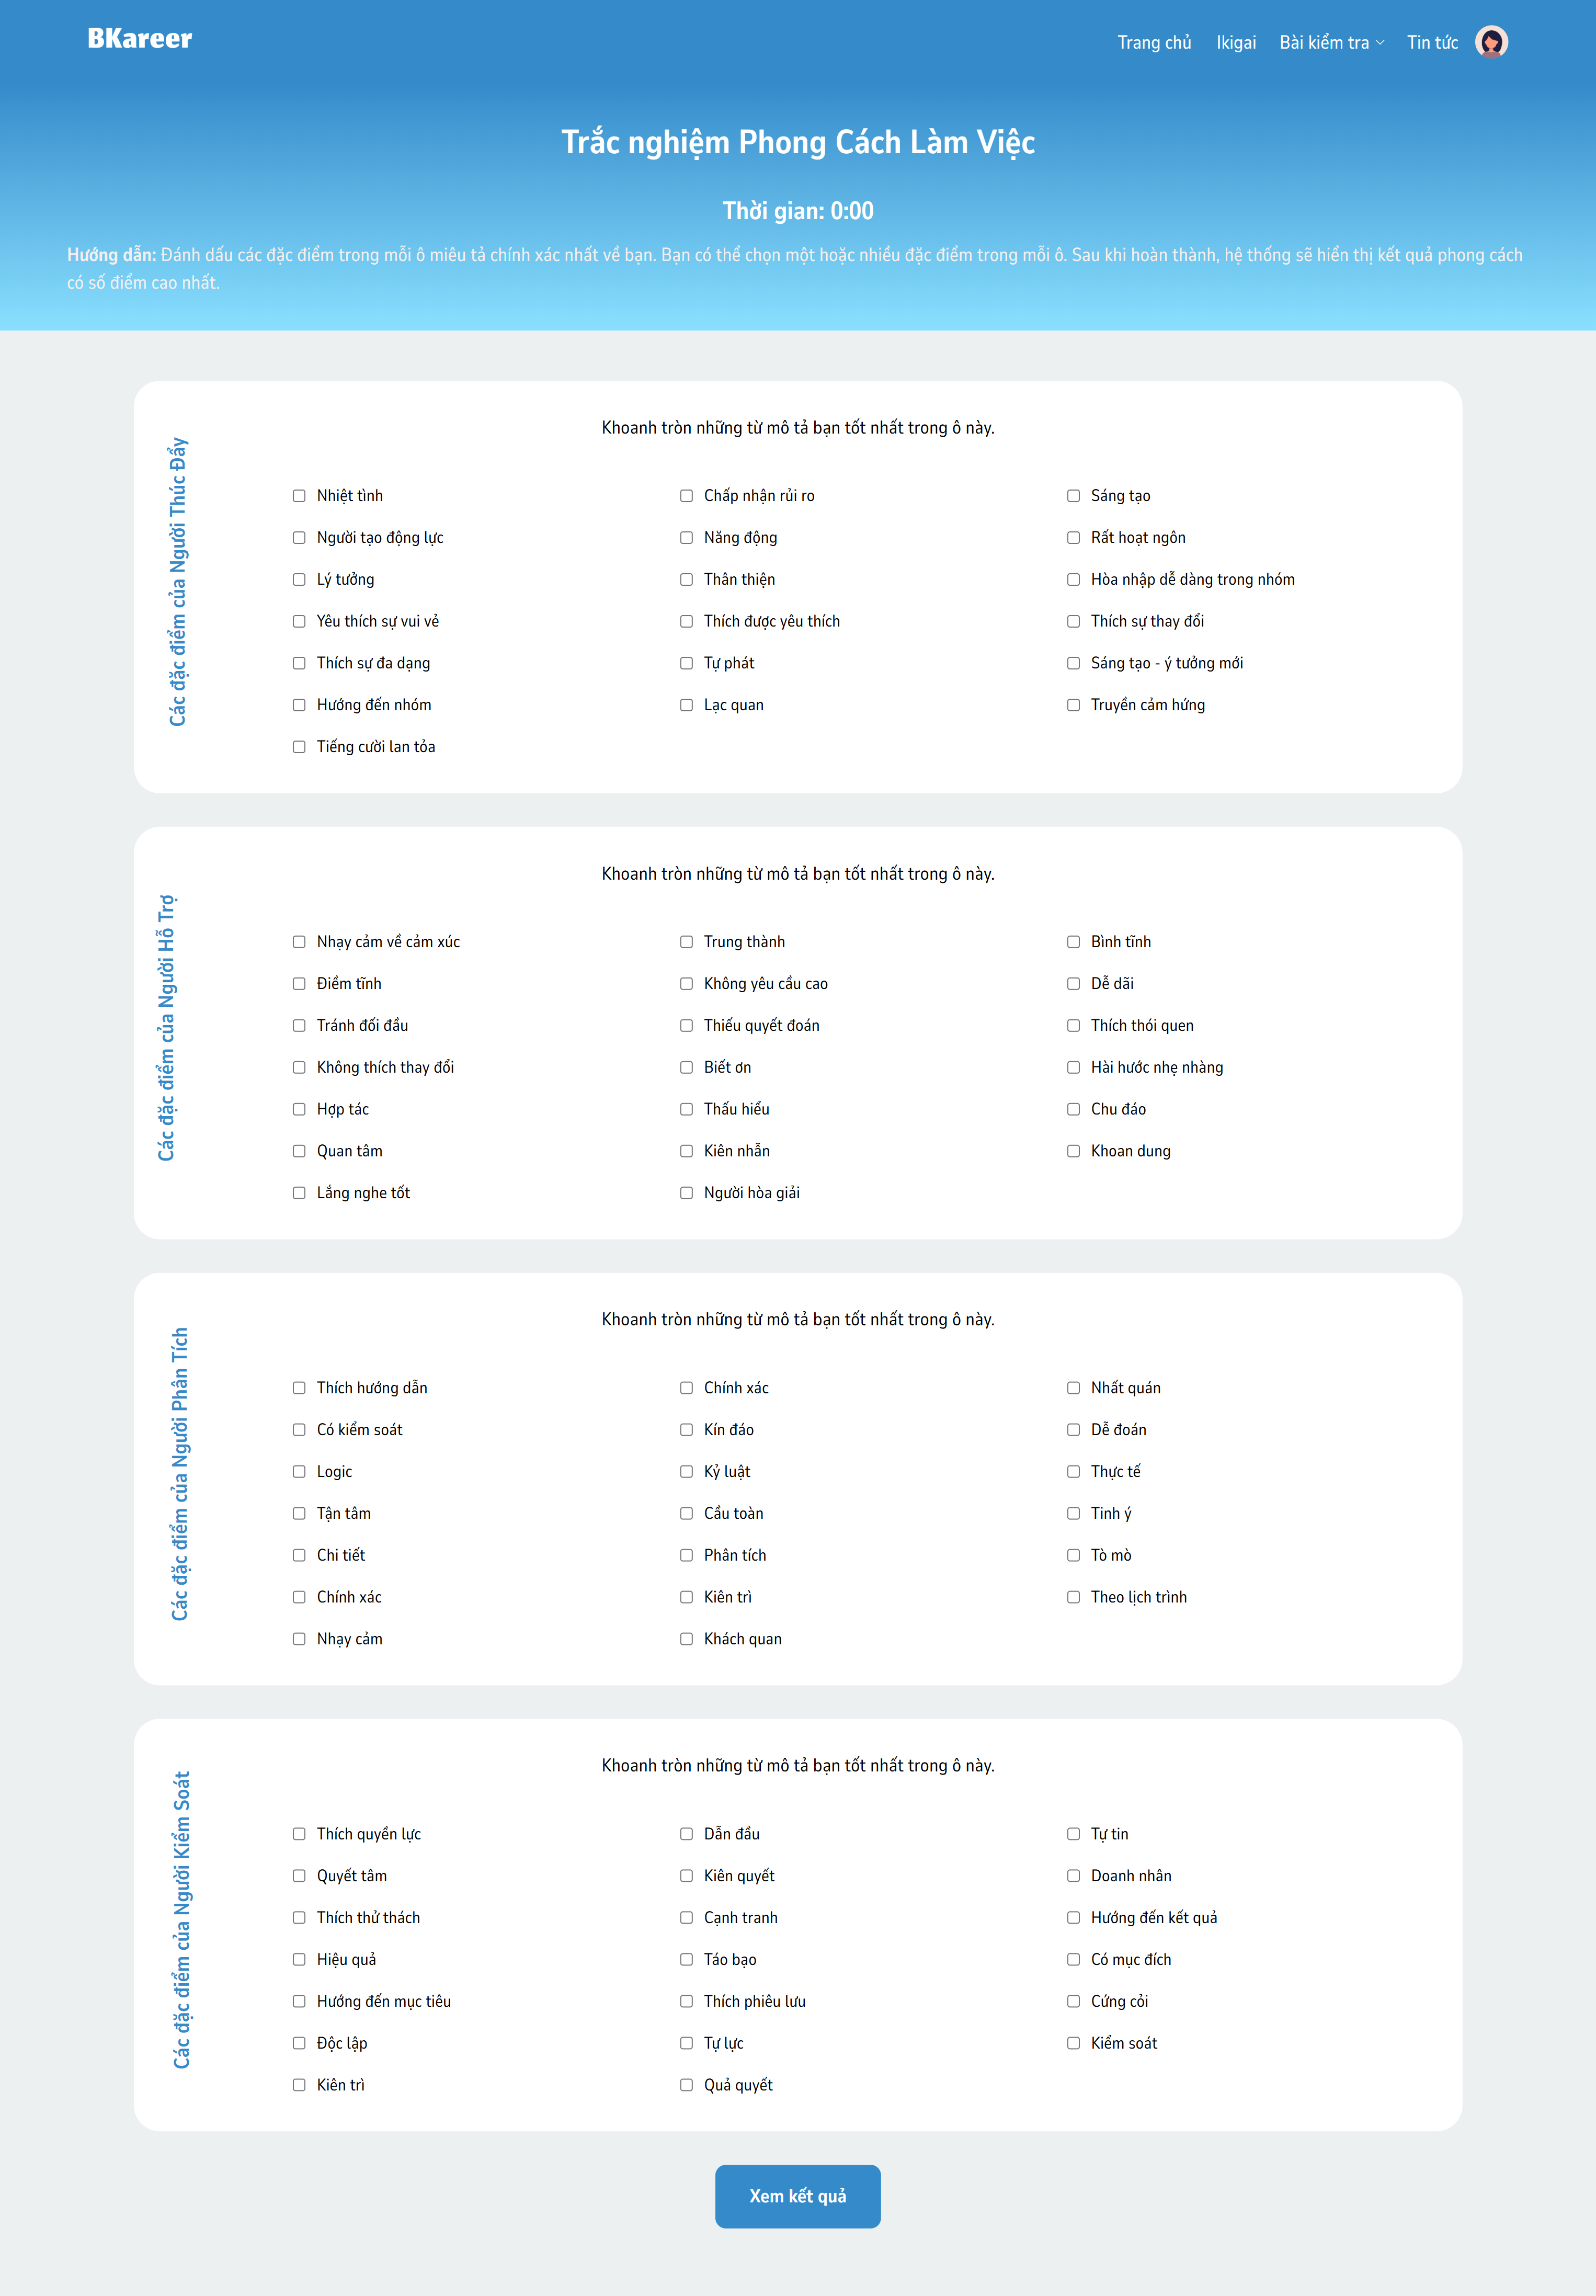
\includegraphics[width=0.8\textwidth]
    {images/chap5/workStyle.png}
    \vspace{0.5cm}
    \caption{Trang thực hiện trắc nghiệm phong cách làm việc}
\end{figure}

Các thành phần chính của trang thực hiện trắc nghiệm phong cách làm việc:
\begin{itemize}
    \item Thanh tiến trình: Bao gồm đồng hồ đếm thời gian thực hiện bài kiểm tra.
    \item Hướng dẫn: Giúp người dùng hiểu rõ hơn về cách thức thực hiện bài kiểm tra để đạt được kết quả chính xác nhất.
    \item Các ô câu hỏi: Mỗi ô bao gồm các lựa chọn có các đặc điểm của từng phong cách tương ứng với mỗi ô, cho phép người dùng chọn các lựa chọn mô tả đúng về bản thân mình, và có thể thay đổi sau khi lựa chọn.
    \item Nút:
        \begin{itemize}
            \item Nút ``Xem kết quả": Hiển thị giao diện thông báo kết quả cho người dùng.
        \end{itemize}
\end{itemize}


%%%%%%%%%% True Colors Detail %%%%%%%%%%
\subsection{Trang giới thiệu trắc nghiệm tính cách True Colors}
Trang giới thiệu trắc nghiệm tính cách True Colors là một nền tảng trực tuyến cung cấp thông tin chi tiết về một công cụ đánh giá tính cách dựa trên bốn màu sắc chính: xanh lá, cam, vàng, và xanh dương. Mô hình True Colors được sử dụng rộng rãi để giúp mọi người hiểu rõ hơn về bản thân, các mối quan hệ và cách tương tác hiệu quả với người khác.

Mục đích của trang giới thiệu trắc nghiệm tính cách True Colors:
\begin{itemize}
    \item Giải thích về mô hình True Colors: Trang web sẽ cung cấp định nghĩa rõ ràng về từng màu sắc, đặc điểm tính cách tương ứng, và cách các màu sắc tương tác với nhau.
    \item Giới thiệu về trắc nghiệm: Giải thích cách thức hoạt động của trắc nghiệm, loại câu hỏi và cách tính điểm để xác định màu sắc chủ đạo và màu sắc hỗ trợ.
    \item Nêu rõ lợi ích của việc xác định màu sắc: Giúp người dùng hiểu rõ hơn về điểm mạnh, điểm yếu, sở thích, phong cách làm việc và cách giao tiếp hiệu quả.
\end{itemize}

\begin{figure}[H]
    \centering
    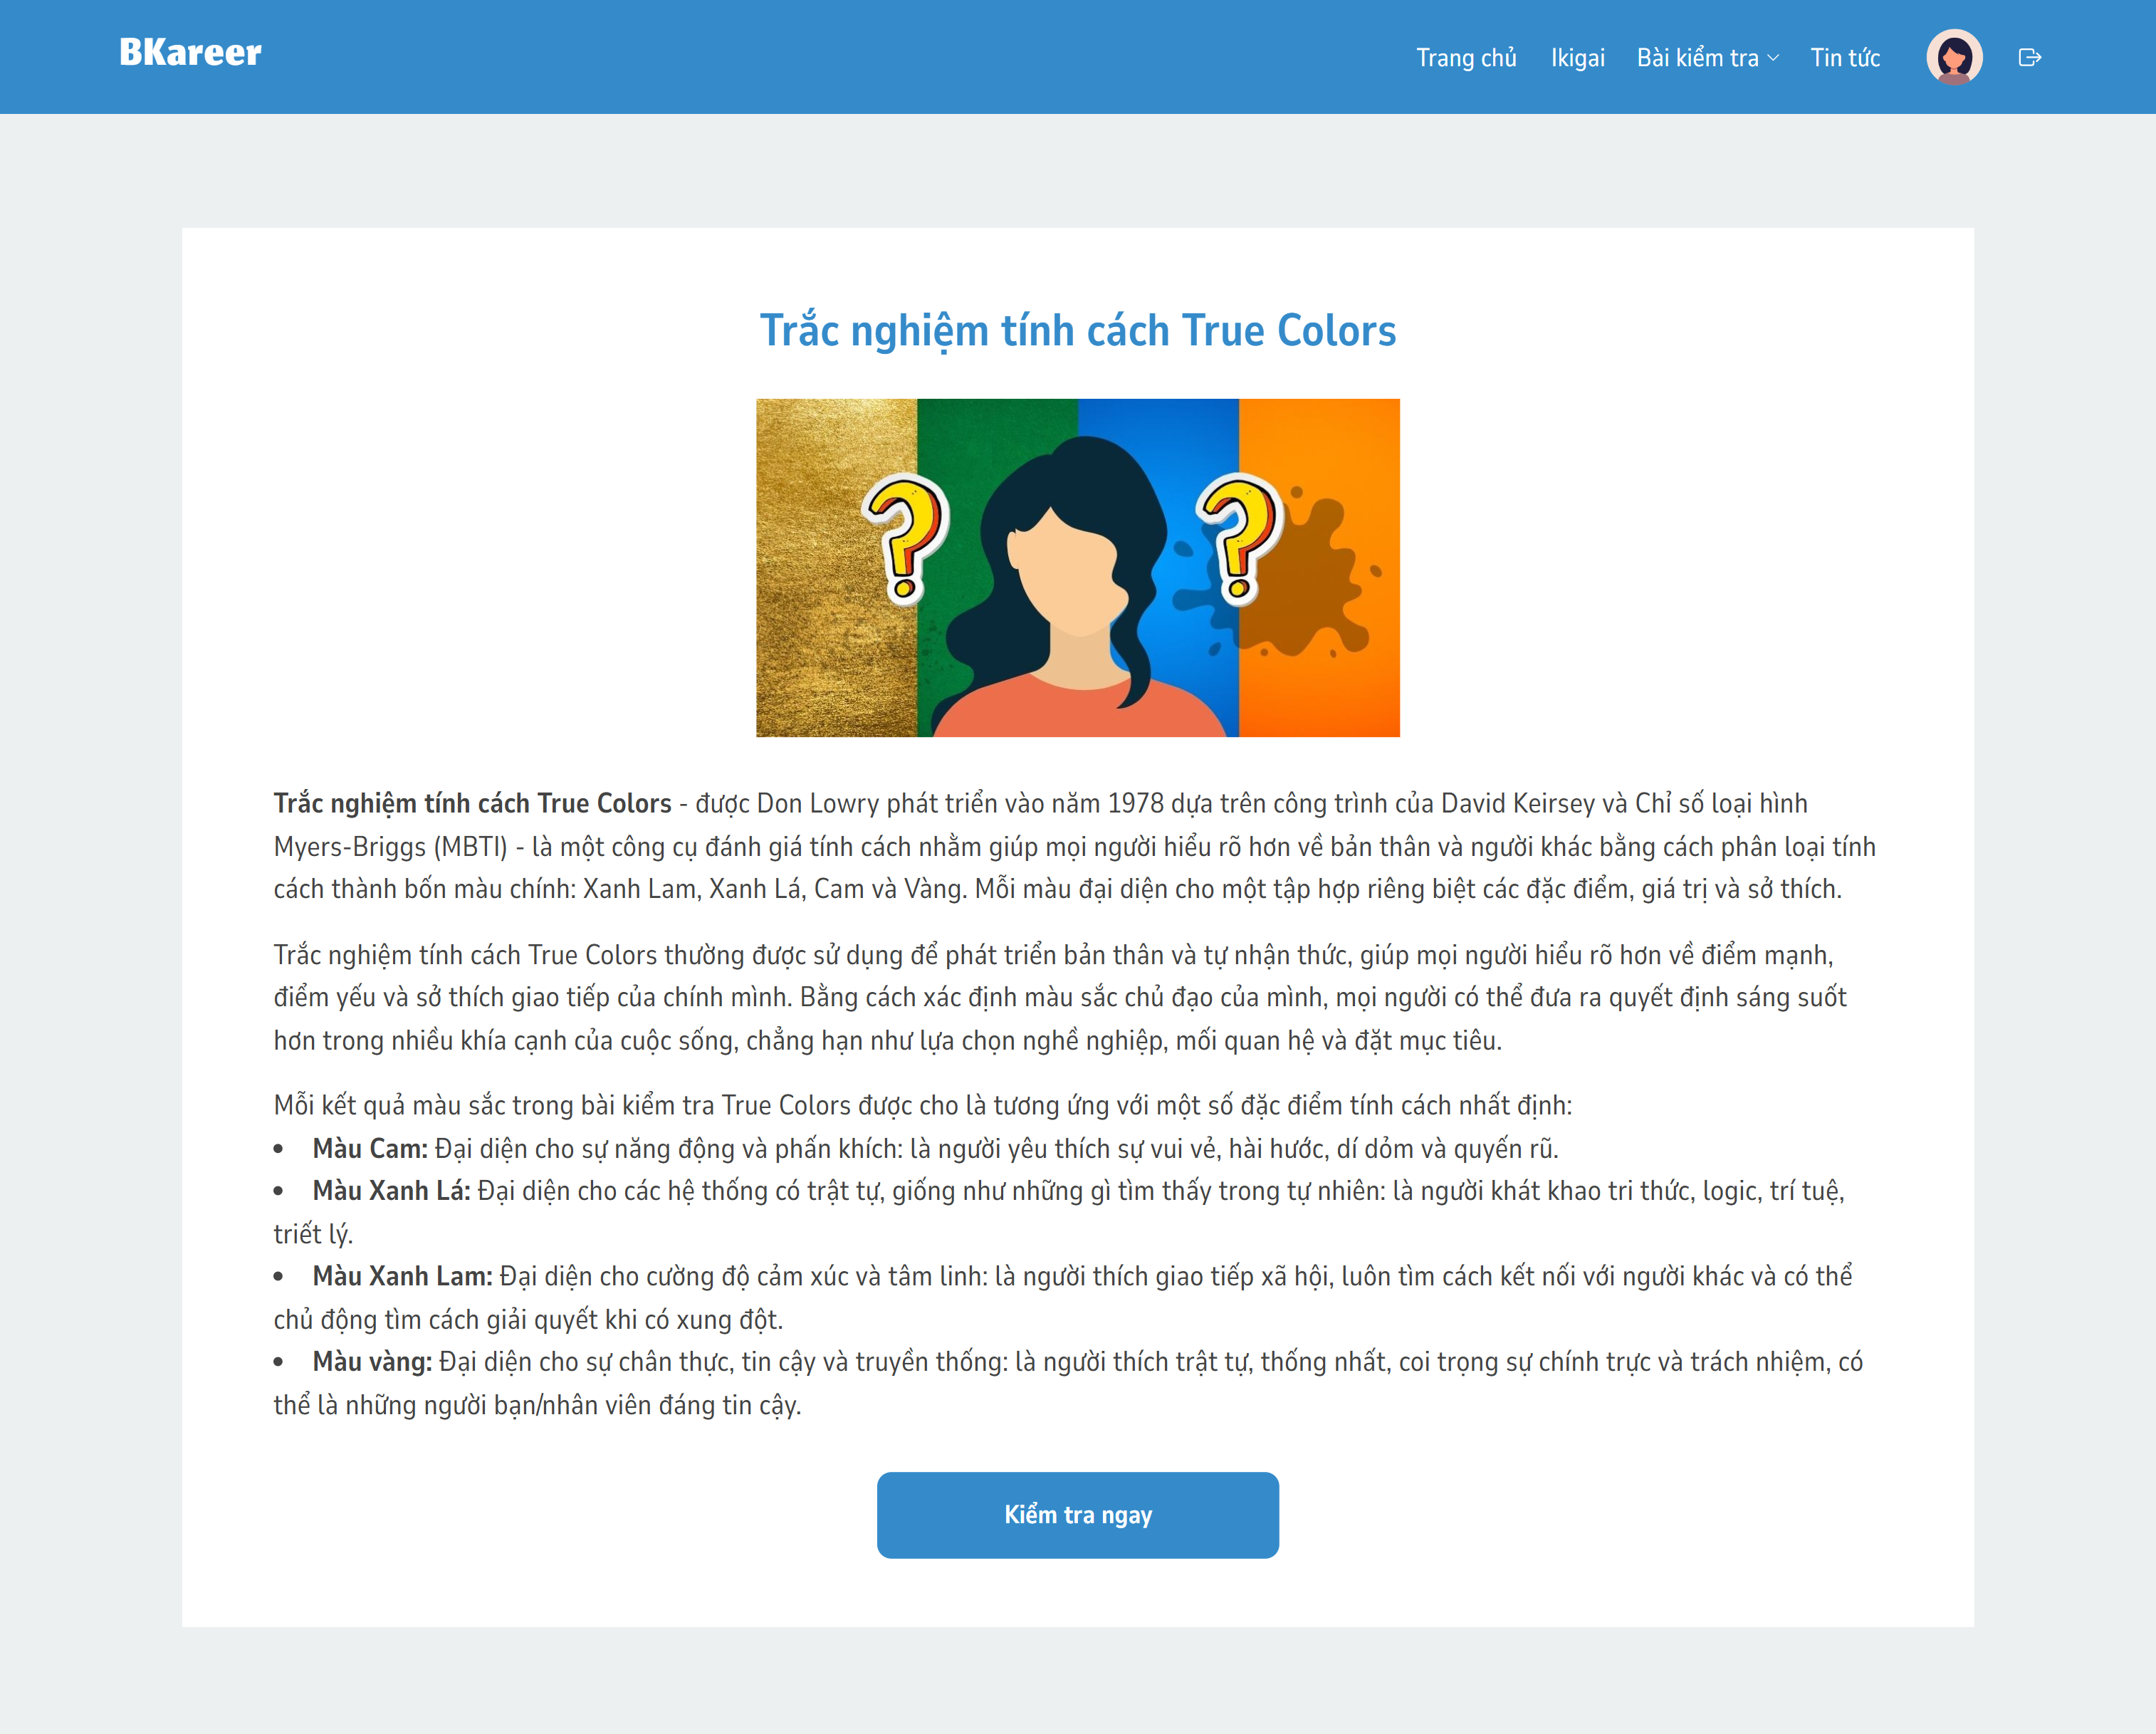
\includegraphics[width=0.8\textwidth]
    {images/chap5/colorsDetail.png}
    \vspace{0.5cm}
    \caption{Trang giới thiệu trắc nghiệm tính cách True Colors}
\end{figure}

Các thành phần chính của trang giới thiệu trắc nghiệm tính cách True Colors:
\begin{itemize}
    \item Hình ảnh minh họa: Hình ảnh minh họa cho nội dung của trang giúp người dùng có thể hình dung sơ lược về trang.
    \item Phần giới thiệu: Phần giới thiệu có vai trò cung cấp thông tin cần thiết cho người dùng, giúp người dùng hiểu rõ hơn về mục đích, nội dung và thành phần bài kiểm tra, từ đó có sự chuẩn bị tốt hơn.
    \item Nút:
        \begin{itemize}
            \item Nút ``Kiểm tra ngay": Cho phép người dùng chuyển đến trang kiểm tra để bắt đầu thực hiện bài kiểm tra ngay lập tức.
        \end{itemize}
\end{itemize}


%%%%%%%%%% True Colors Test %%%%%%%%%%
\subsection{Trang thực hiện trắc nghiệm tính cách True Colors}
Trang thực hiện trắc nghiệm tính cách True Colors là một nền tảng trực tuyến được thiết kế để giúp người dùng khám phá và hiểu rõ hơn về tính cách của bản thân dựa trên mô hình True Colors. Mô hình này chia tính cách của con người thành 4 màu sắc cơ bản, mỗi màu đại diện cho một nhóm tính cách với những đặc điểm, sở trường và thách thức riêng biệt.

Mục đích của trang thực hiện trắc nghiệm tính cách True Colors:
\begin{itemize}
    \item Đánh giá tính cách: Cung cấp một công cụ để người dùng tự đánh giá tính cách của mình một cách khách quan.
    \item Hiểu rõ bản thân: Giúp người dùng nhận biết điểm mạnh, điểm yếu, sở thích, và xu hướng hành vi của mình.
    \item Ứng dụng vào cuộc sống: Đưa ra gợi ý về việc lựa chọn nghề nghiệp, xây dựng mối quan hệ, và phát triển bản thân dựa trên kết quả trắc nghiệm.
    \item Tìm hiểu về tâm lý: Giới thiệu về mô hình True Colors và cách nó được ứng dụng trong cuộc sống.
\end{itemize}

\begin{figure}[H]
    \centering
    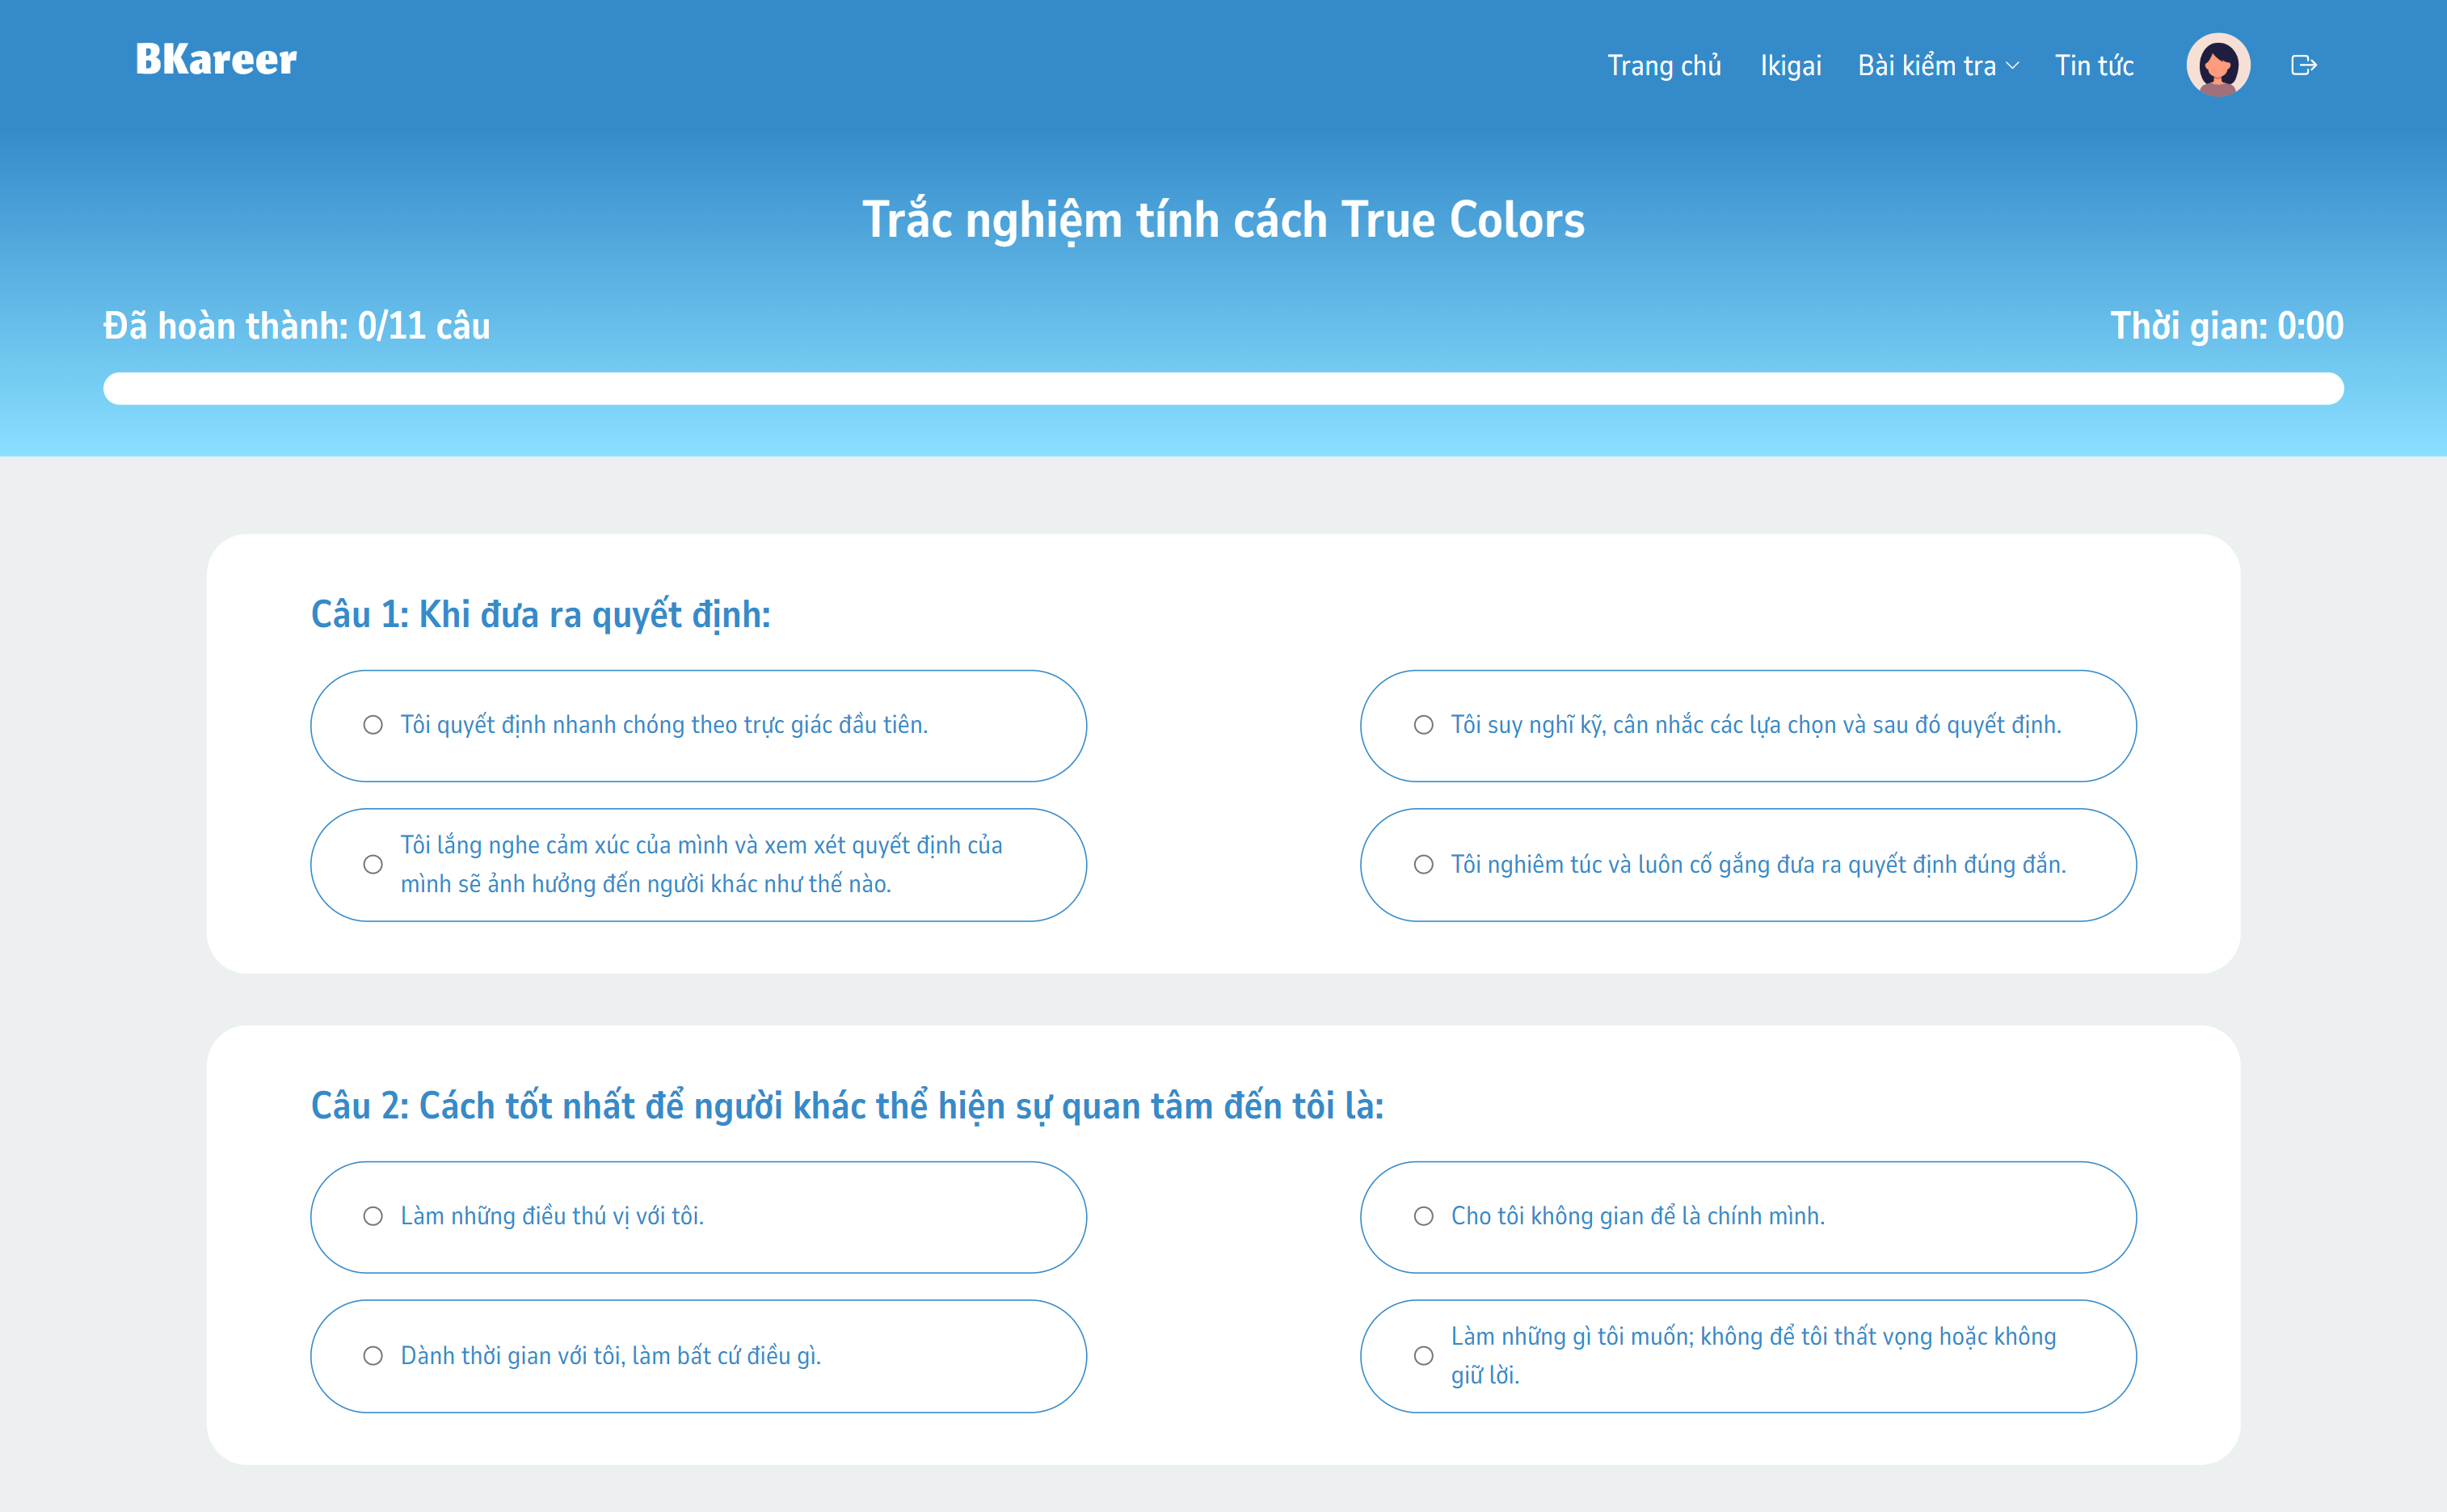
\includegraphics[width=0.8\textwidth]
    {images/chap5/trueColors.png}
    \vspace{0.5cm}
    \caption{Trang thực hiện trắc nghiệm tính cách True Colors}
\end{figure}

Các thành phần chính của trang thực hiện trắc nghiệm tính cách True Colors:
\begin{itemize}
    \item Thanh tiến trình: Bao gồm tiến độ hoàn thành bài kiểm tra và đồng hồ đếm thời gian thực hiện bài kiểm tra.
    \item Các khối câu hỏi: Mỗi khối bao gồm 1 câu hỏi và 4 đáp án, cho phép người dùng chọn 1 trong 4 đáp án phù hợp nhất với mình, và có thể thay đổi sau khi lựa chọn.
    \item Nút:
        \begin{itemize}
            \item Nút ``Xem kết quả": Hiển thị giao diện thông báo kết quả cho người dùng.
        \end{itemize}
\end{itemize}


%%%%%%%%%% Grit Scale Detail %%%%%%%%%%
\subsection{Trang giới thiệu trắc nghiệm thang đo bền chí}
Trang giới thiệu trắc nghiệm thang đo bền chí là một nền tảng trực tuyến cung cấp thông tin chi tiết về một công cụ đánh giá giúp người dùng hiểu rõ hơn về mức độ bền chí của bản thân. Bền chí là một phẩm chất quan trọng, liên quan đến khả năng kiên trì theo đuổi mục tiêu, vượt qua khó khăn và thất bại để đạt được thành công.

Mục đích của trang giới thiệu trắc nghiệm thang đo bền chí:
\begin{itemize}
    \item Giải thích về bền chí: Trang web sẽ cung cấp định nghĩa rõ ràng về bền chí, tầm quan trọng của bền chí trong cuộc sống và công việc.
    \item Giới thiệu về trắc nghiệm: Giải thích cách thức hoạt động của trắc nghiệm, loại câu hỏi và cách tính điểm.
    \item Nêu rõ lợi ích của việc xác định mức độ bền chí: Giúp người dùng hiểu rõ hơn về điểm mạnh, điểm yếu của bản thân trong việc kiên trì theo đuổi mục tiêu, từ đó tìm ra cách cải thiện.
\end{itemize}

\begin{figure}[H]
    \centering
    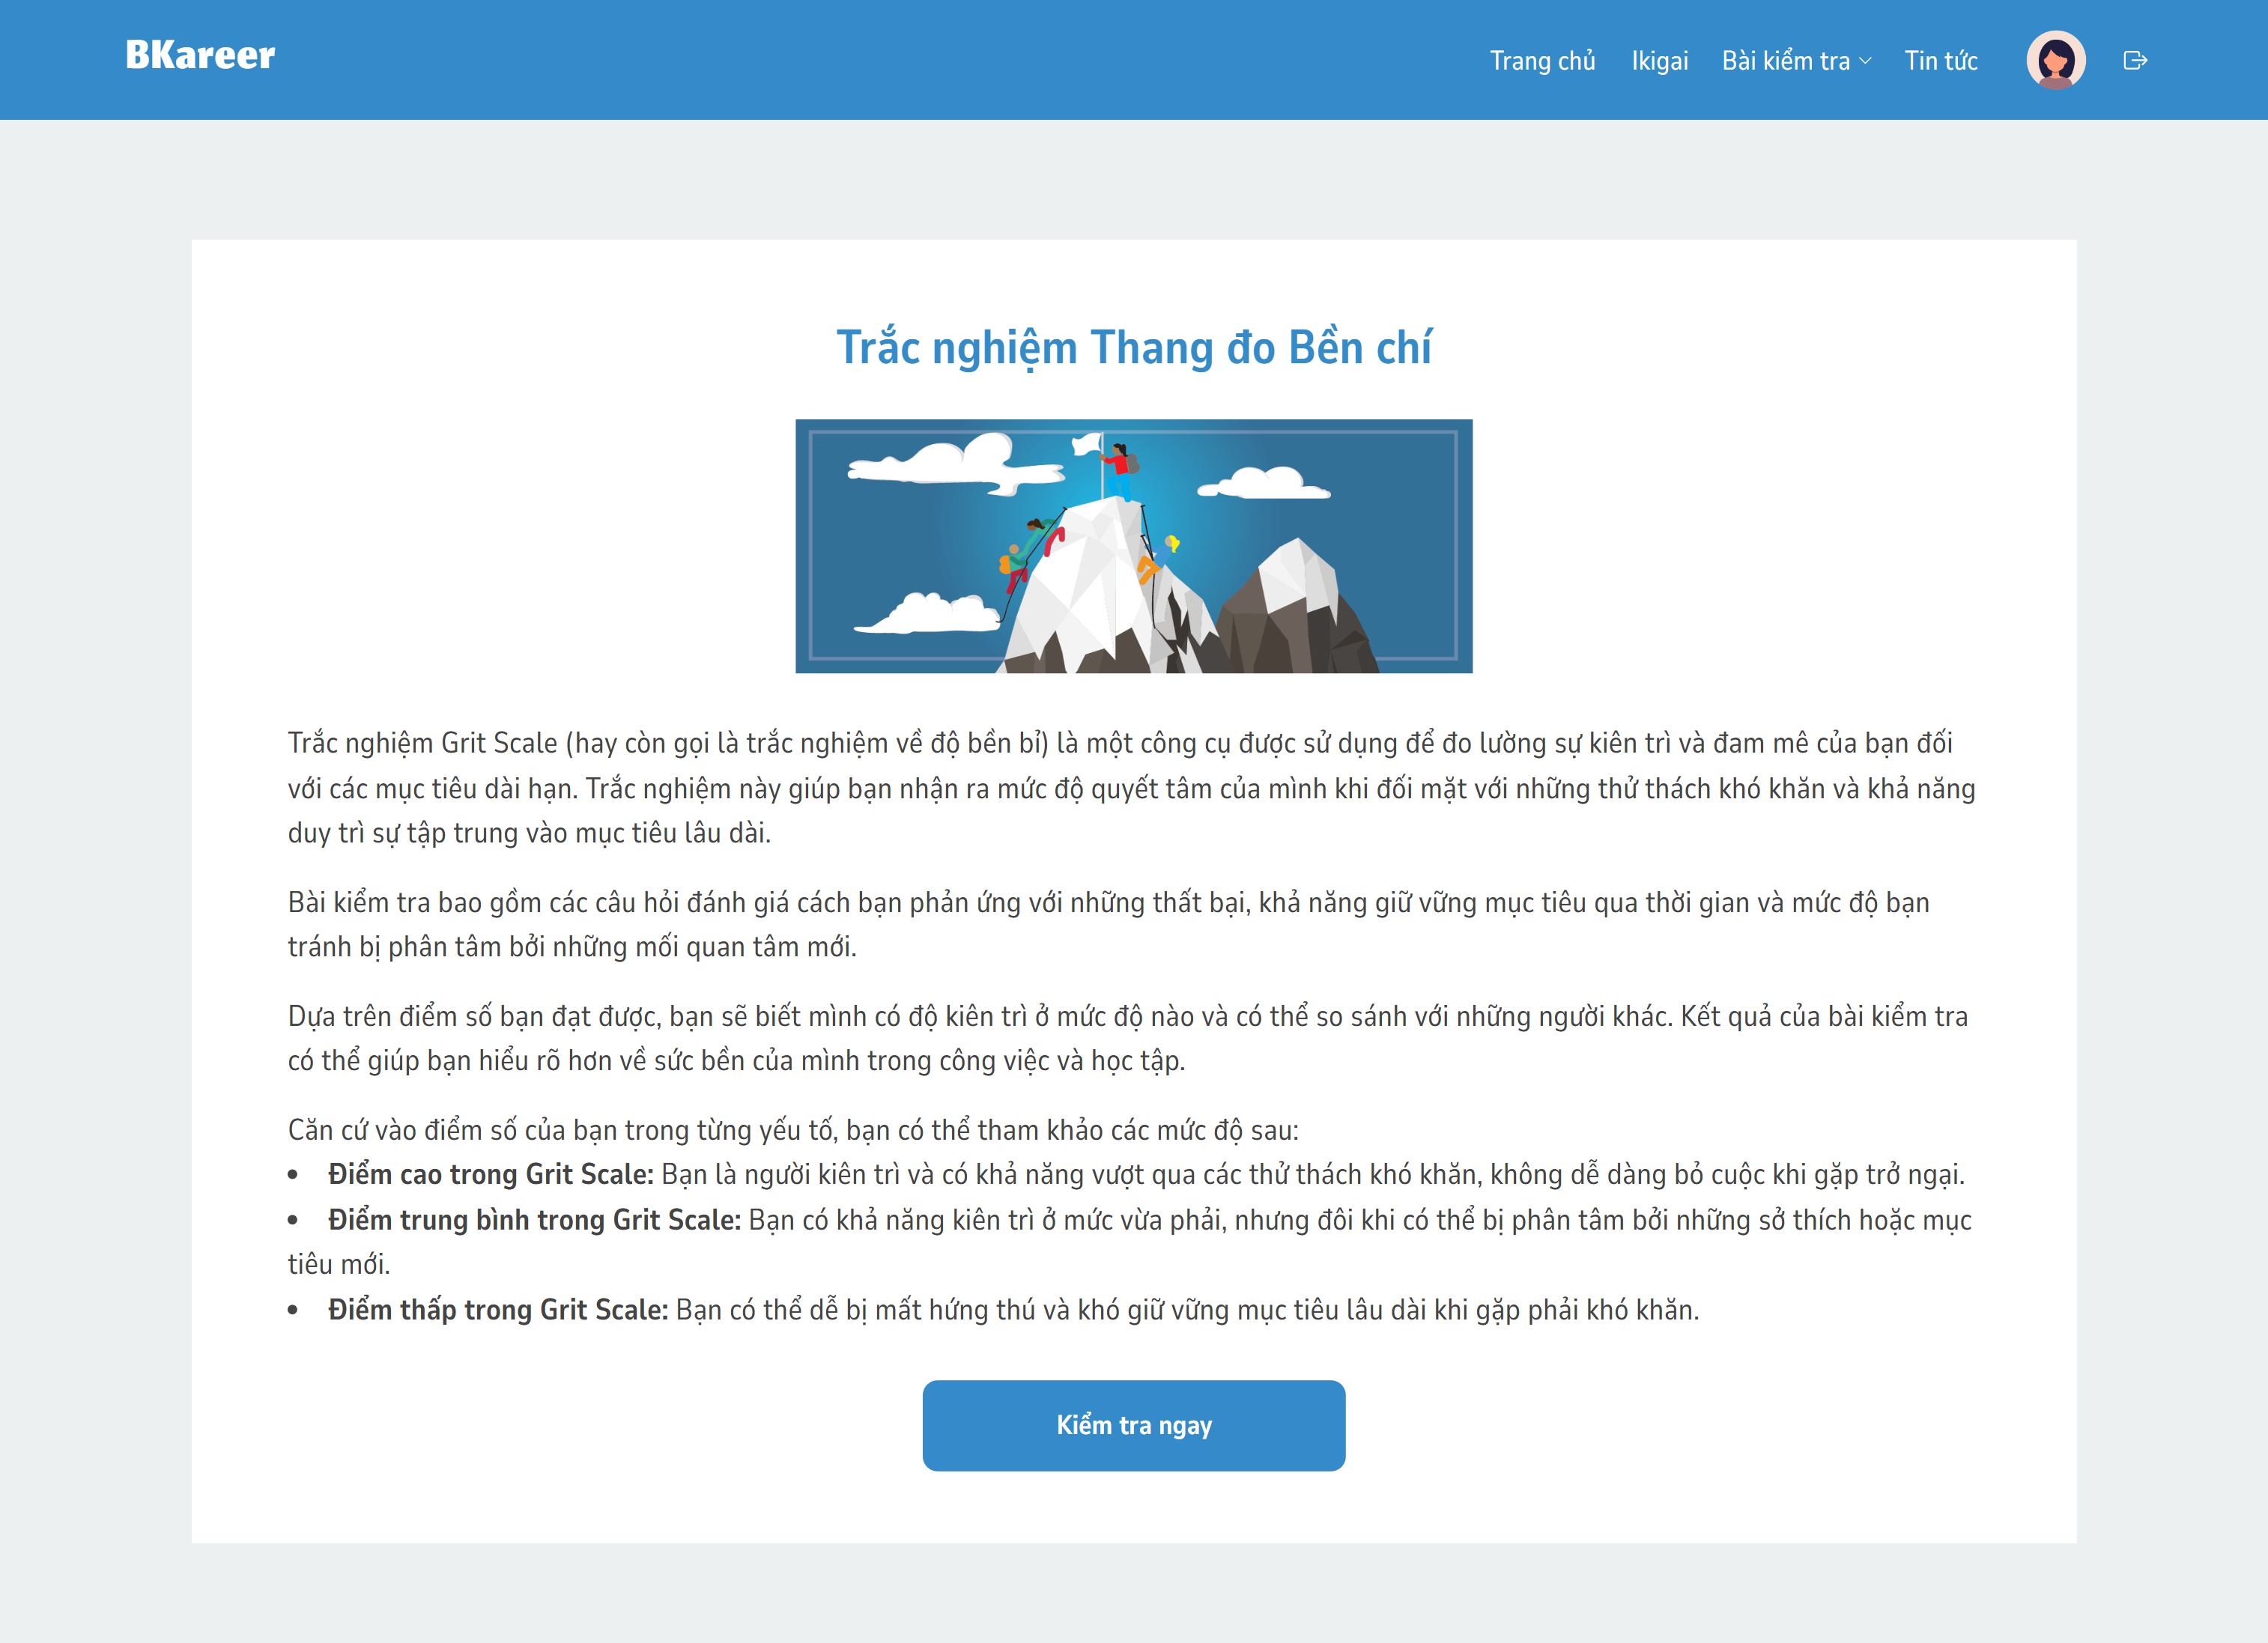
\includegraphics[width=0.8\textwidth]{images/chap5/gritDetail.png}
    \vspace{0.5cm}
    \caption{Trang giới thiệu trắc nghiệm thang đo bền chí}
\end{figure}

Các thành phần chính của trang giới thiệu trắc nghiệm thang đo bền chí:
\begin{itemize}
    \item Hình ảnh minh họa: Hình ảnh minh họa cho nội dung của trang giúp người dùng có thể hình dung sơ lược về trang.
    \item Phần giới thiệu: Phần giới thiệu có vai trò cung cấp thông tin cần thiết cho người dùng, giúp người dùng hiểu rõ hơn về mục đích, nội dung và thành phần bài kiểm tra, từ đó có sự chuẩn bị tốt hơn.
    \item Nút:
        \begin{itemize}
            \item Nút ``Kiểm tra ngay": Cho phép người dùng chuyển đến trang kiểm tra để bắt đầu thực hiện bài kiểm tra ngay lập tức.
        \end{itemize}
\end{itemize}


%%%%%%%%%% Grit Scale Test %%%%%%%%%%
\subsection{Trang thực hiện trắc nghiệm thang đo bền chí}
Trang thực hiện trắc nghiệm thang đo bền chí là một nền tảng trực tuyến được thiết kế để giúp người dùng đánh giá mức độ bền bỉ của bản thân. Bền chí (Grit) là sự kết hợp giữa đam mê và sự kiên trì theo đuổi mục tiêu dài hạn, một yếu tố quan trọng góp phần vào thành công trong cuộc sống.

Mục đích của trang thực hiện trắc nghiệm thang đo bền chí:
\begin{itemize}
    \item Đánh giá mức độ bền chí: Cung cấp một công cụ để người dùng tự đánh giá mức độ bền bỉ của bản thân.
    \item Hiểu rõ bản thân: Giúp người dùng nhận biết điểm mạnh, điểm yếu liên quan đến sự bền bỉ.
    \item Tìm kiếm phương pháp cải thiện: Đưa ra các gợi ý, phương pháp để tăng cường sự bền bỉ.
    \item Ứng dụng vào cuộc sống: Giúp người dùng xác định mục tiêu và lên kế hoạch thực hiện một cách hiệu quả.
\end{itemize}

\begin{figure}[H]
    \centering
    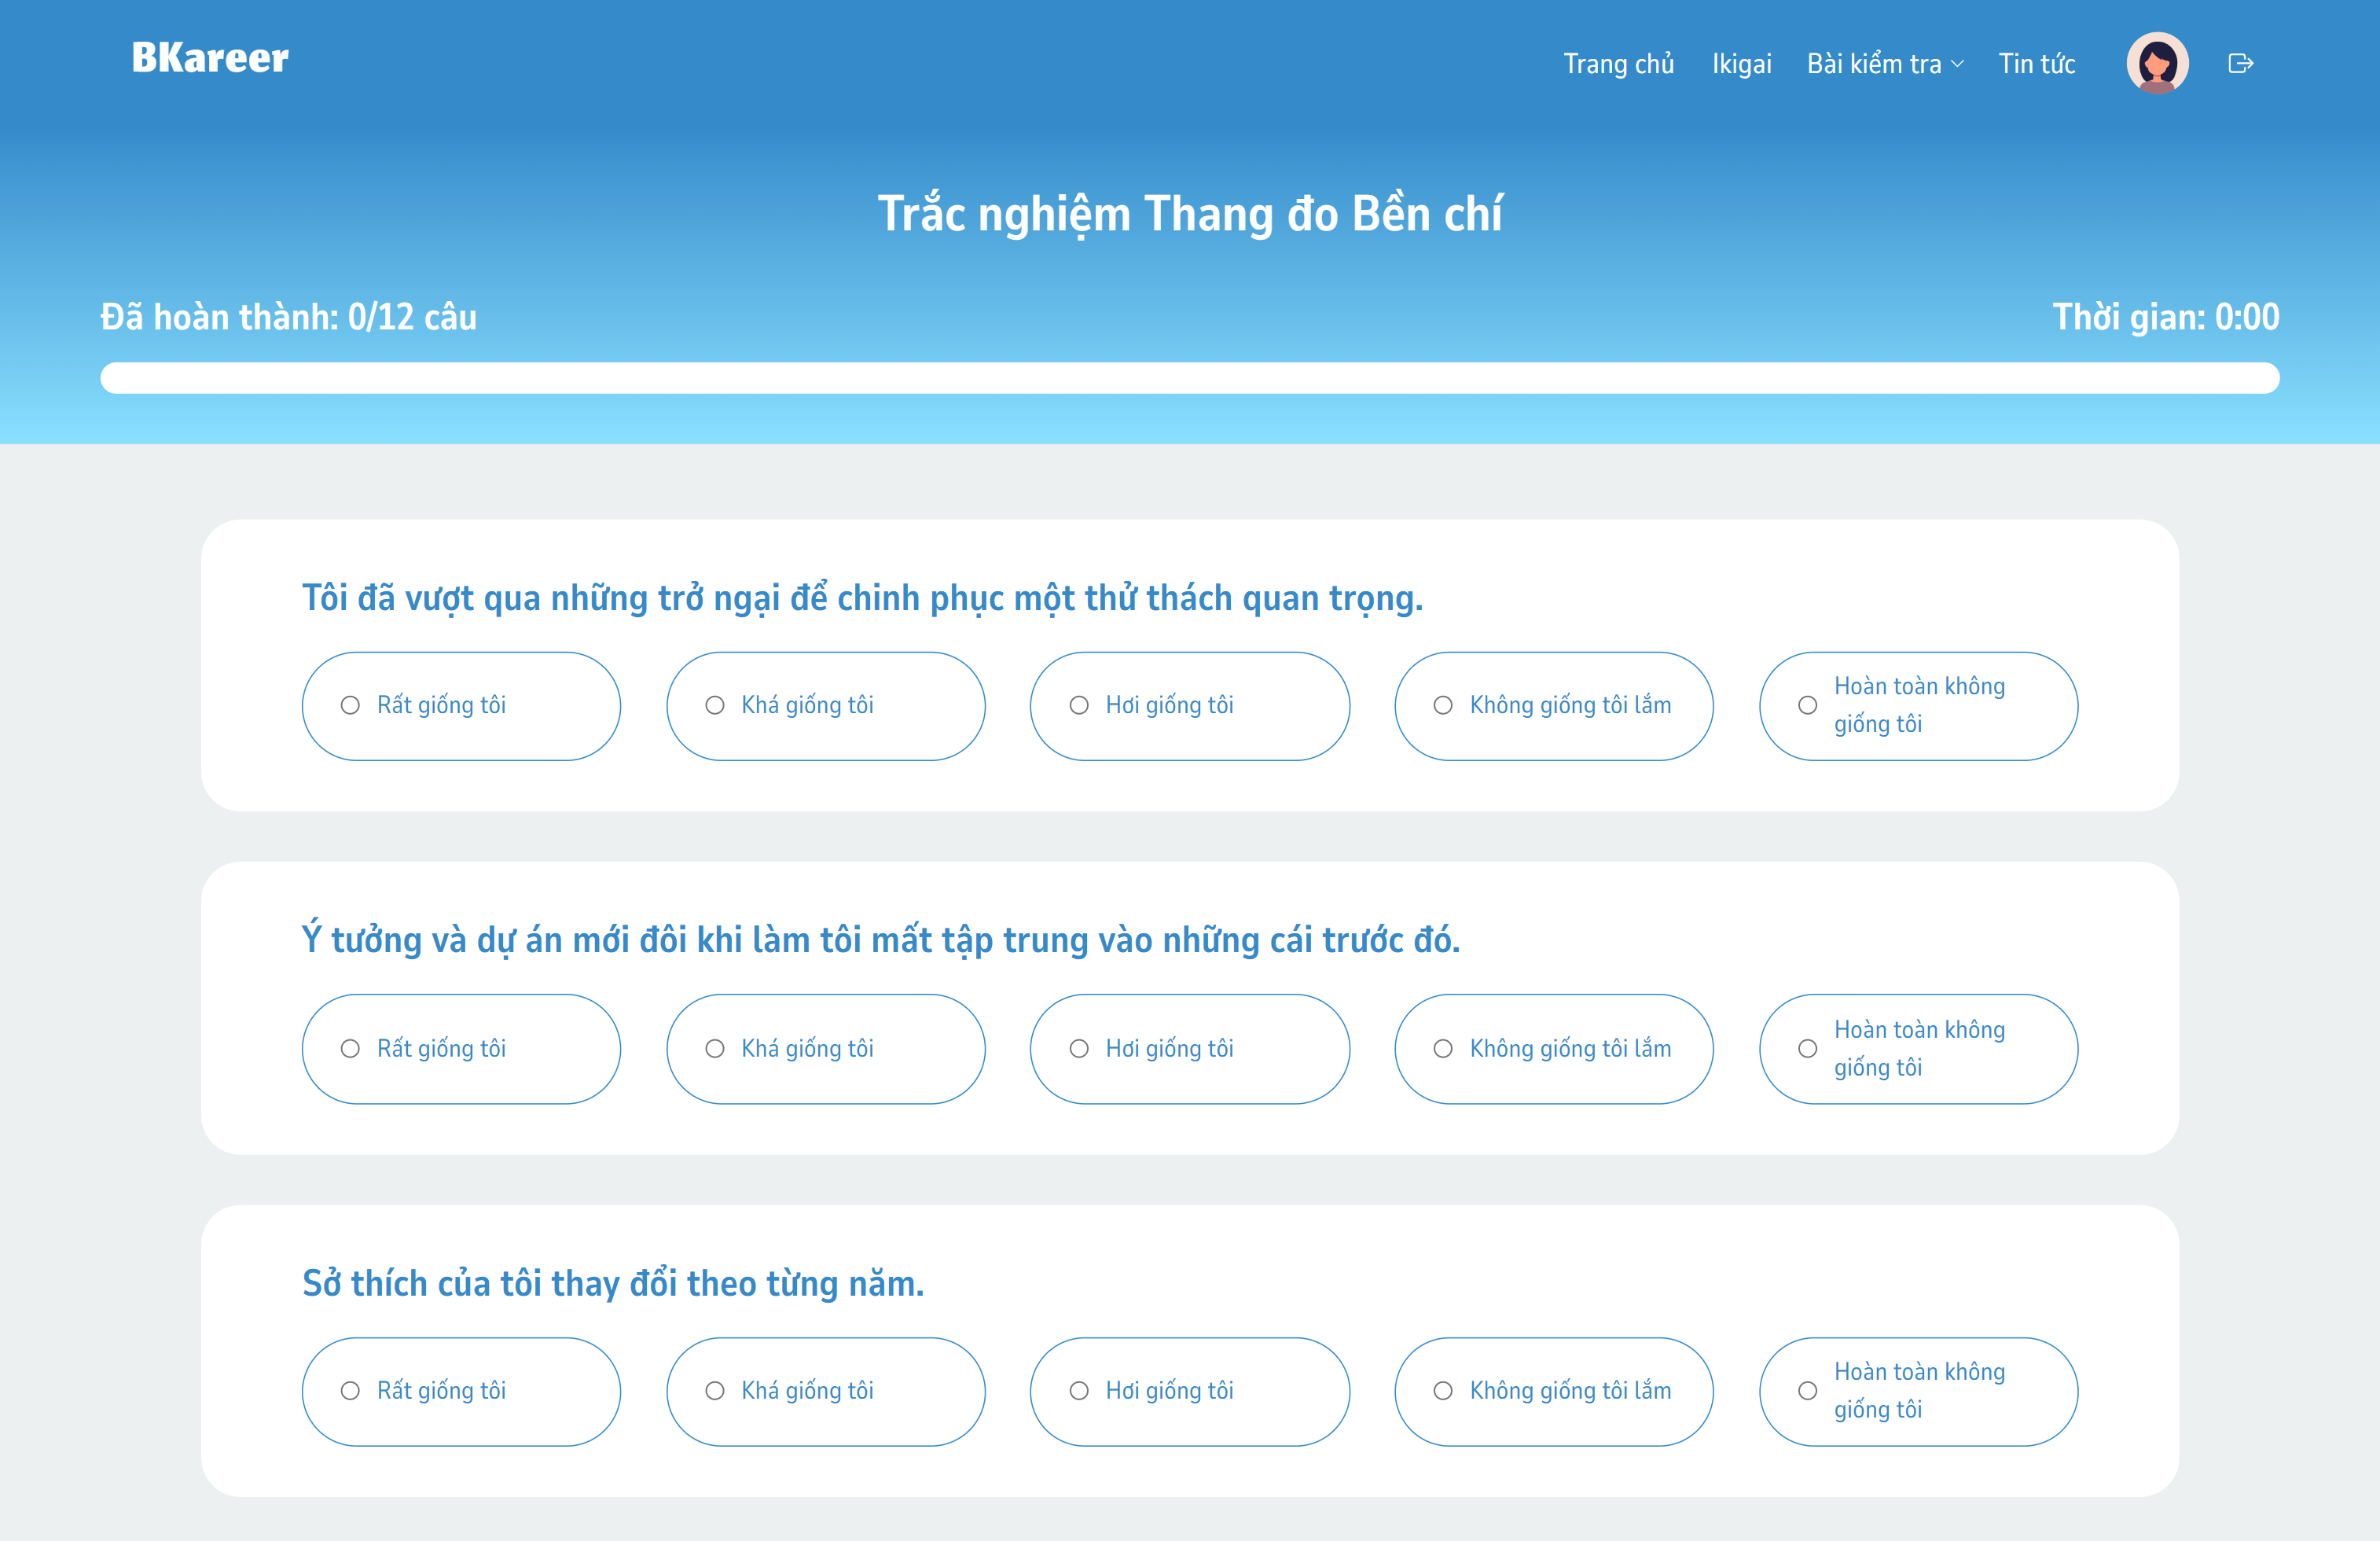
\includegraphics[width=0.8\textwidth]
    {images/chap5/gritTest.png}
    \vspace{0.5cm}
    \caption{Trang thực hiện trắc nghiệm thang đo bền chí}
\end{figure}

Các thành phần chính của trang thực hiện trắc nghiệm thang đo bền chí:
\begin{itemize}
    \item Thanh tiến trình: Bao gồm tiến độ hoàn thành bài kiểm tra và đồng hồ đếm thời gian thực hiện bài kiểm tra.
    \item Các khối câu hỏi: Mỗi khối bao gồm 1 câu hỏi và 5 đáp án theo mức độ từ hoàn toàn không giống tôi đến rất giống tôi, cho phép người dùng chọn 1 trong 5 đáp án đúng nhất khi nói về bản thân, và có thể thay đổi sau khi lựa chọn.
    \item Nút:
        \begin{itemize}
            \item Nút ``Xem kết quả": Hiển thị giao diện thông báo kết quả cho người dùng.
        \end{itemize}
\end{itemize}


%%%%%%%%%%%%%%%%%%%%%%%%%%%% Admin Dashboard %%%%%%%%%%%%%%%%%%%%%%%%%%%%
\section{Admin Dashboard}
\subsection{Trang đăng nhập}

\begin{figure}[H]
    \centering
    
\includegraphics[width=0.8\linewidth]{images/dashboardLogin.png}
    \vspace{0.6cm}
    \caption{Trang đăng nhập cho Admin Dashboard}
\end{figure}

Sau khi đăng nhập vào tài khoản dành cho Admin, hệ thống chuyển hướng qua trang tổng quan dashboard.

\subsection{Tổng quan dashboard}

\begin{figure}[H]
    \centering
    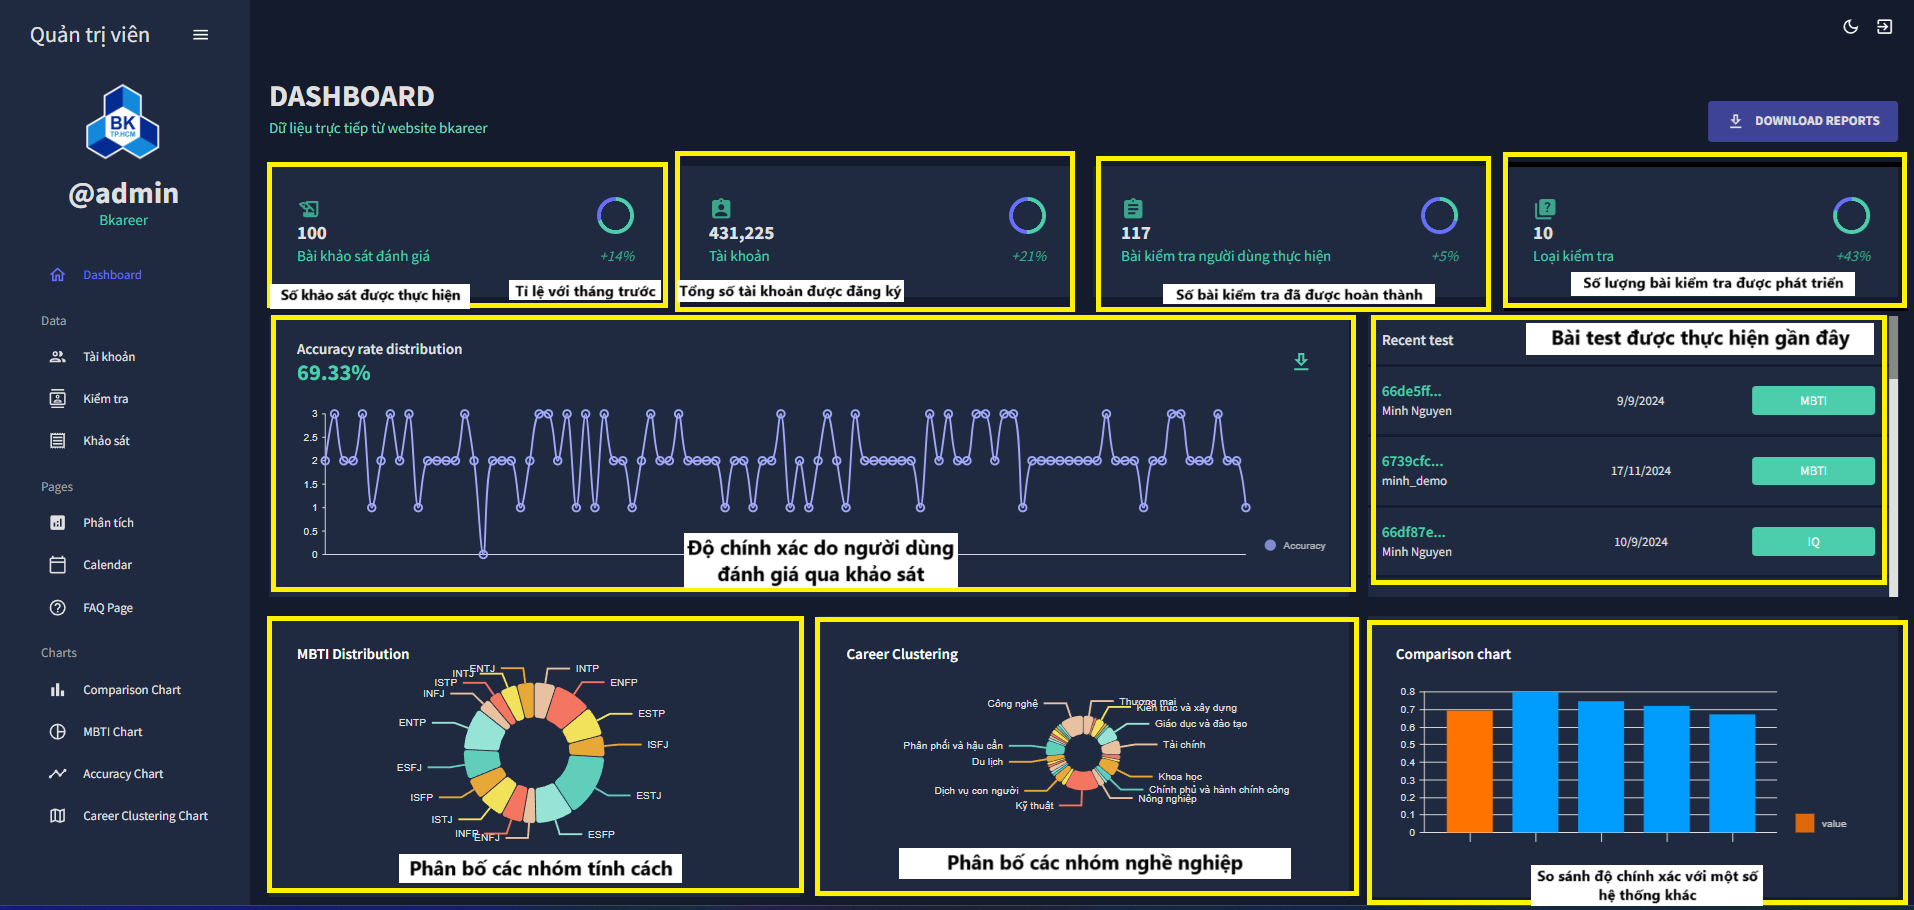
\includegraphics[width=0.9\linewidth]{images/dashboard.png}
    \vspace{0.6cm}
    \caption{Trang tổng quan dashboard}
\end{figure}

Trang dashboard của hệ thống bao gồm các thành phần chính như sau:
\begin{itemize}
    \item Số lượng bài khảo sát đã được thực hiện, bao gồm tỷ lệ tăng giảm so với tháng trước.
    \item Tổng số tài khoản người dùng đã đăng ký và tỷ lệ tăng trưởng.
    \item Số bài kiểm tra đã được hoàn thành bởi người dùng.
    \item Loại bài kiểm tra đã được phát triển.
    \item Độ chính xác do người dùng đánh giá qua khảo sát (biểu đồ phân phối độ chính xác).
    \item Phân bố các nhóm tính cách dựa trên MBTI.
    \item Phân bố các nhóm nghề nghiệp từ kết quả Career Clustering.
    \item Biểu đồ so sánh độ chính xác với một số hệ thống khác.
    \item Danh sách các bài test được thực hiện gần đây.
\end{itemize}

Ngoài ra, thanh điều hướng bên trái cung cấp liên kết đến các trang chức năng khác, bao gồm:
\begin{itemize}
    \item \nameref{sec:account_management}: Quản lý tài khoản người dùng.
    \item \nameref{sec:test_management}: Quản lý kết quả kiểm tra
    \item \nameref{sec:survey_management}: Quản lý khảo sát người dùng
    % \item \nameref{sec:analysis}: Phân tích dữ liệu.
    % \item \nameref{sec:calendar}: Lịch làm việc.
    % \item \nameref{sec:faq}: Trang câu hỏi thường gặp (FAQ).
    \item \nameref{sec:charts}: Các biểu đồ so sánh và phân tích.
\end{itemize}

Các phần tiếp theo sẽ mô tả chi tiết từng trang tương ứng với các mục trên thanh sidebar.

\subsection{Quản lý tài khoản người dùng}
\label{sec:account_management}
\begin{figure}[H]
    \centering
    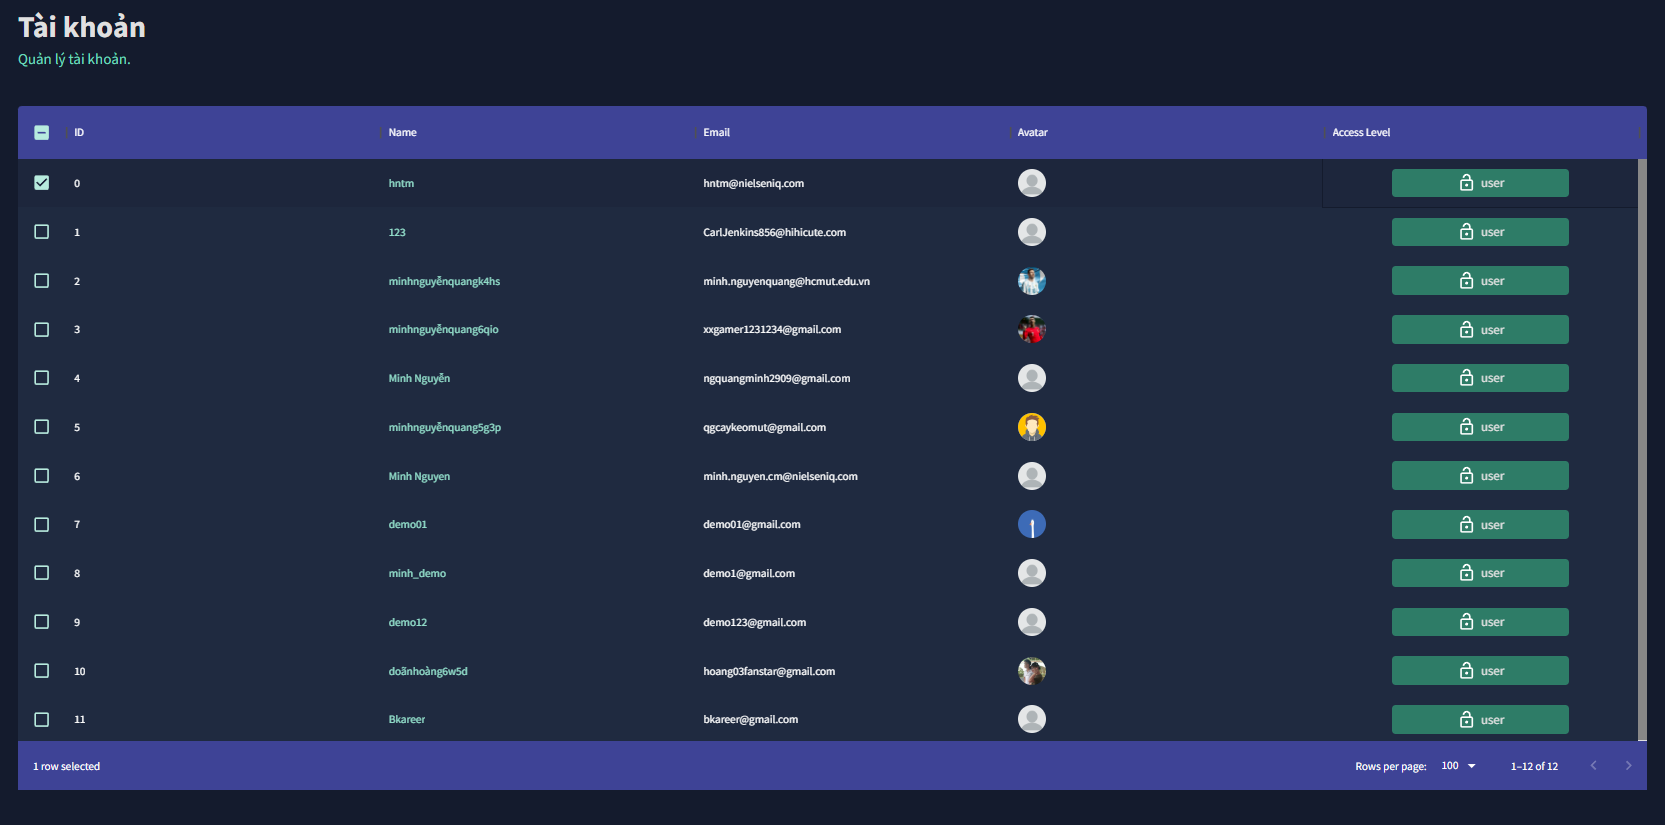
\includegraphics[width=0.75\linewidth]{images/accAdmin.png}
    \vspace{0.6cm}
    \caption{Giao diện quản lý tài khoản người dùng}
\end{figure}

Trang này cho phép quản trị viên thực hiện các thao tác như:
\begin{itemize}
    \item Tìm kiếm, thêm, chỉnh sửa, hoặc xóa tài khoản người dùng.
    \item Xem thông tin chi tiết của từng tài khoản.
    \item Quản lý quyền truy cập và vai trò của người dùng trong hệ thống.
\end{itemize}

\subsection{Quản lý kết quả kiểm tra}
\label{sec:test_management}
\begin{figure}[H]
    \centering
    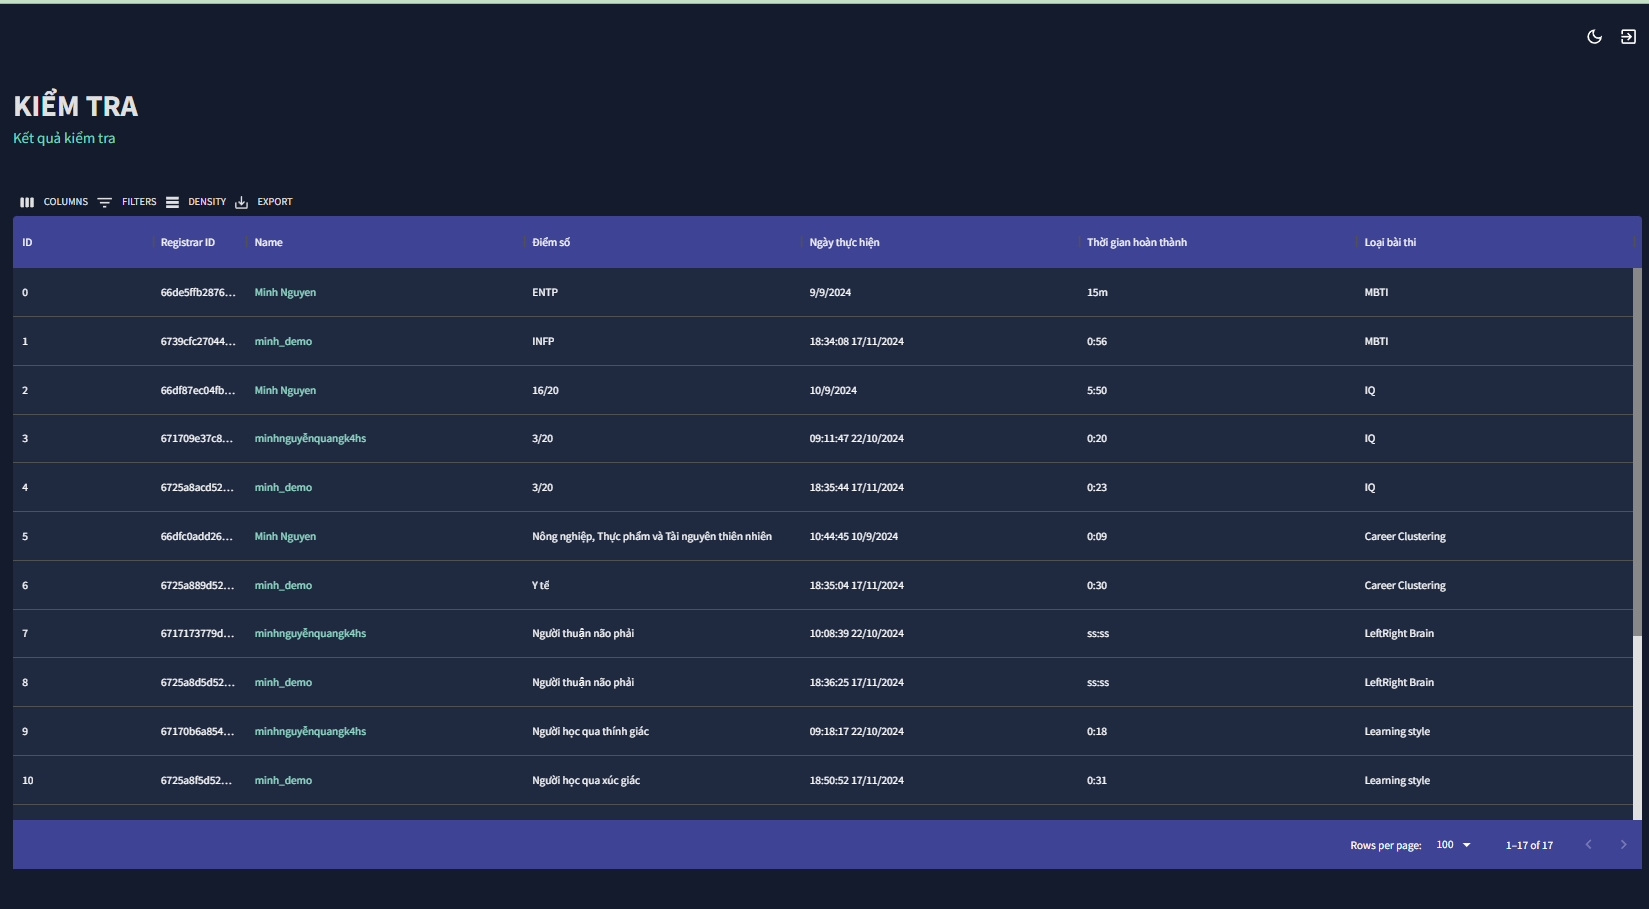
\includegraphics[width=0.75\linewidth]{images/testAdmin.png}
    \vspace{0.6cm}
    \caption{Giao diện quản lý kết quả kiểm tra}
\end{figure}

Trang này tập trung vào việc quản lý các bài kiểm tra và khảo sát, bao gồm:
\begin{itemize}
    \item Lấy dữ liệu kết quả bài kiểm tra để sử dụng cho các chức năng khác 
    \item Xuất dữ liệu ra các loại file khác
\end{itemize}

\subsection{Quản lý khảo sát người dùng}
\label{sec:survey_management}
\begin{figure}[H]
    \centering
    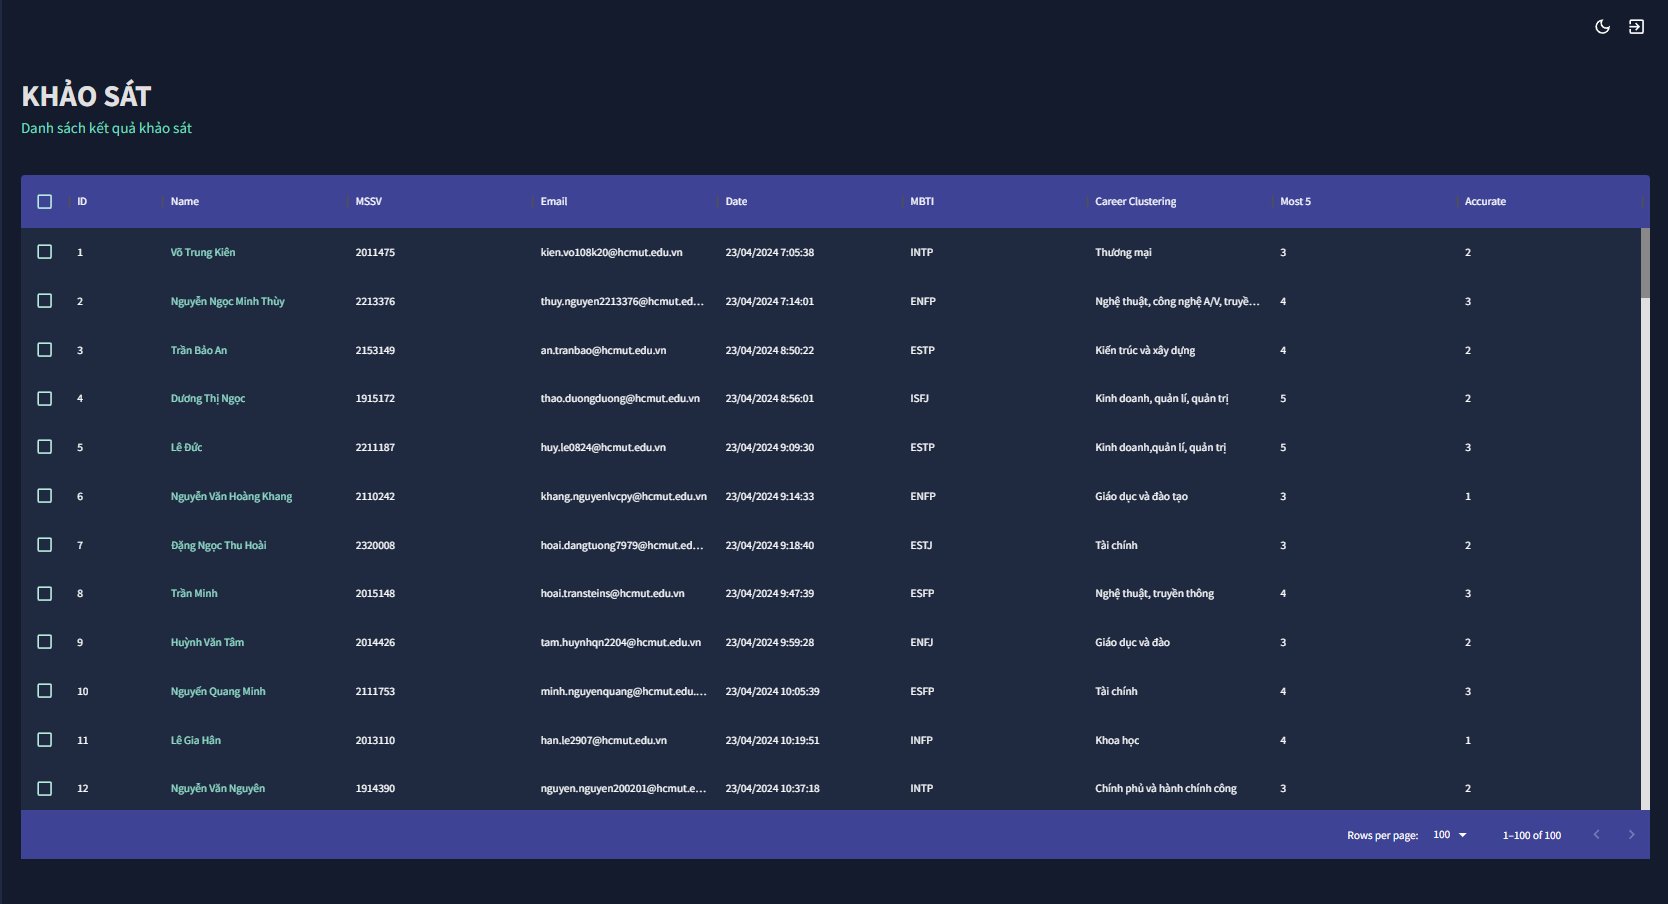
\includegraphics[width=0.75\linewidth]{images/surAdmin.png}
    \vspace{0.6cm}
    \caption{Giao diện quản lý khảo sát người dùng}
\end{figure}

Trang này cho phép quản trị viên thực hiện các chức năng quản lý liên quan đến khảo sát, bao gồm:
\begin{itemize}
    \item Theo dõi số lượng người tham gia và tỷ lệ hoàn thành cho từng khảo sát.
    \item Sử dụng kết quả khảo sát để tính toán độ chính xác của hệ thống dựa trên thực nghiệm người dùng
\end{itemize}

Trang này đóng vai trò quan trọng trong việc thu thập thông tin từ người dùng và phân tích các phản hồi, hỗ trợ quá trình cải tiến hệ thống trang web.

\subsection{Các biểu đồ so sánh và phân tích}
\label{sec:charts}
\subsubsection{Độ chính xác của hệ thống}

\begin{figure}[H]
    \centering
    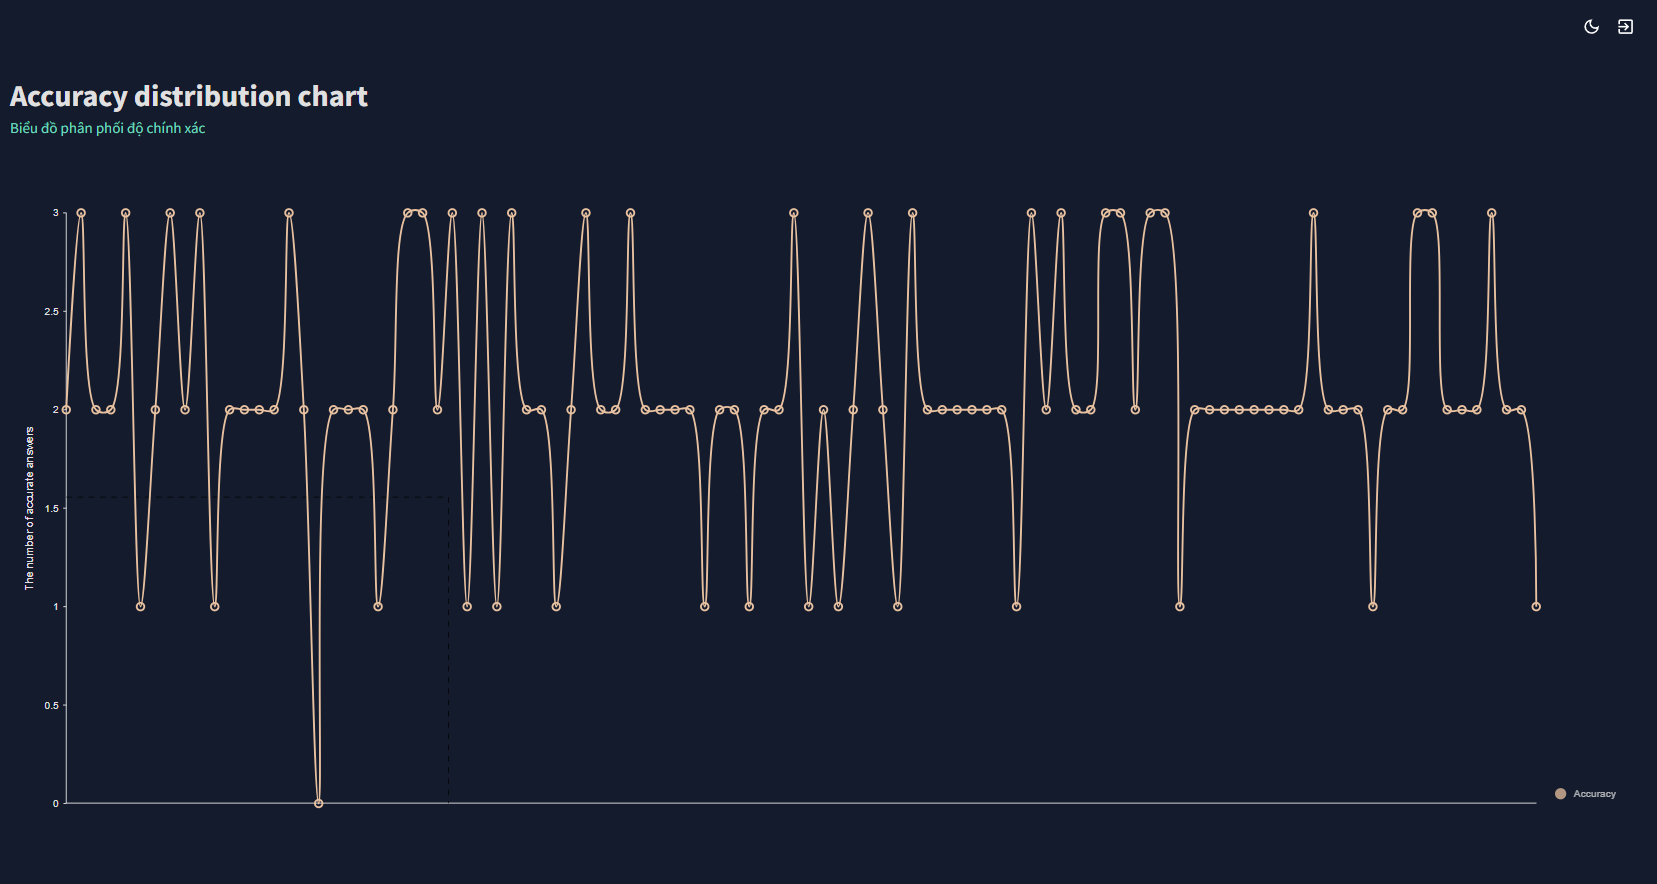
\includegraphics[width=0.75\linewidth]{images/accu.png}
    \vspace{0.6cm}
    \caption{Độ chính xác của hệ thống do người dùng đánh giá}
\end{figure}

\begin{figure}[H]
    \centering
    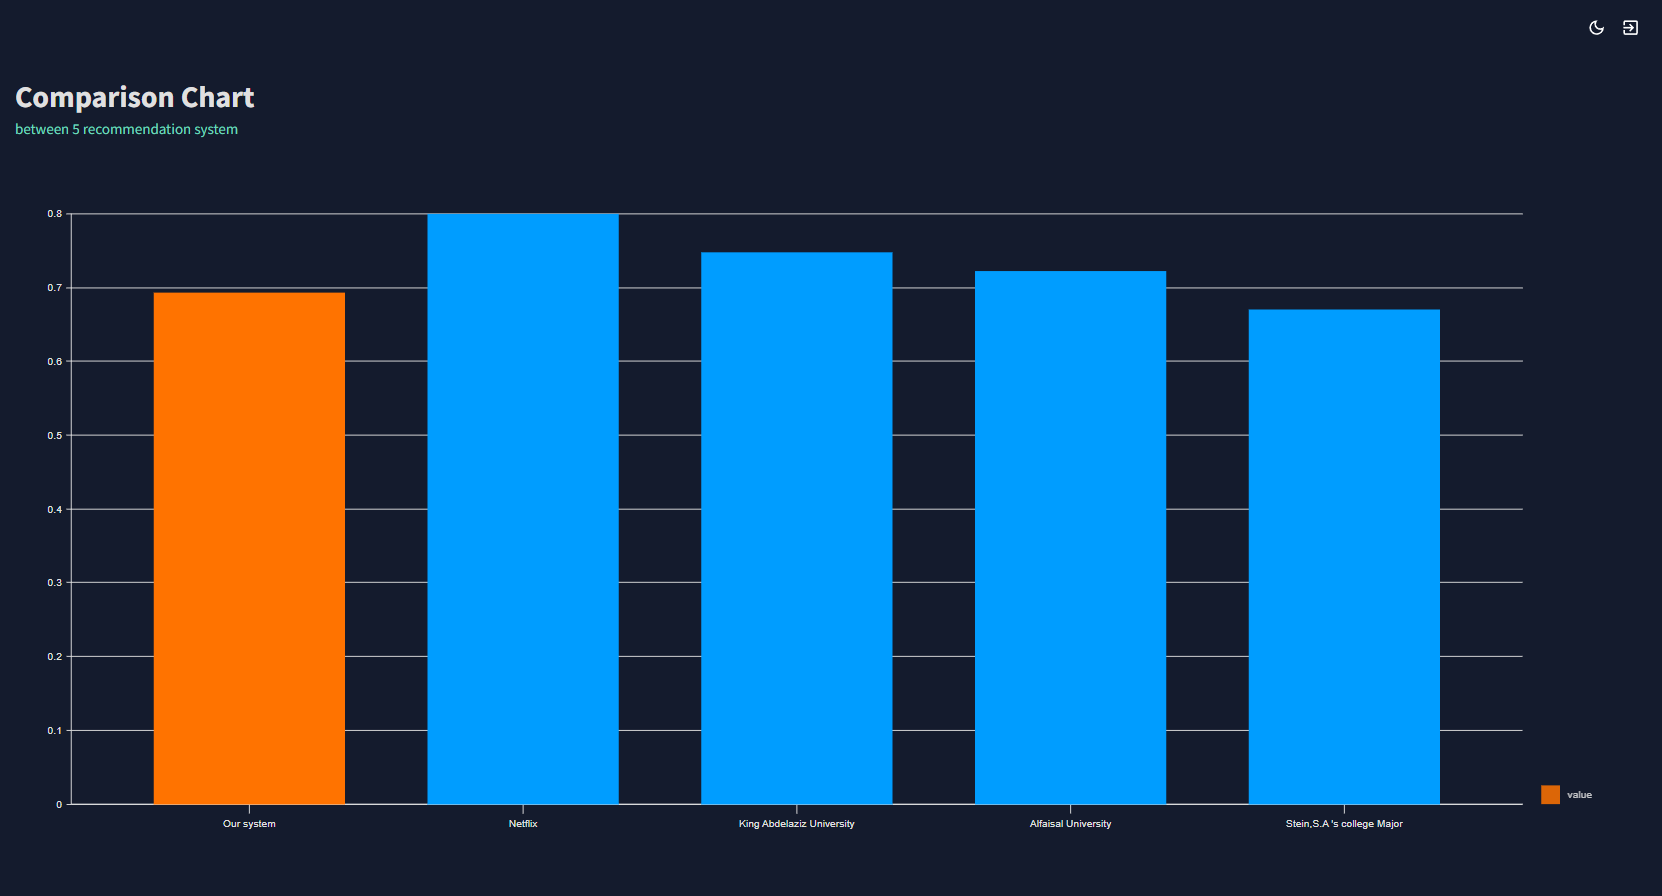
\includegraphics[width=0.75\linewidth]{images/compare.png}
    \vspace{0.6cm}
    \caption{Biểu đồ so sánh độ chính xác với các hệ thống tương tự}
\end{figure}

\subsubsection{Biểu đồ MBTI}
\begin{figure}[H]
    \centering
    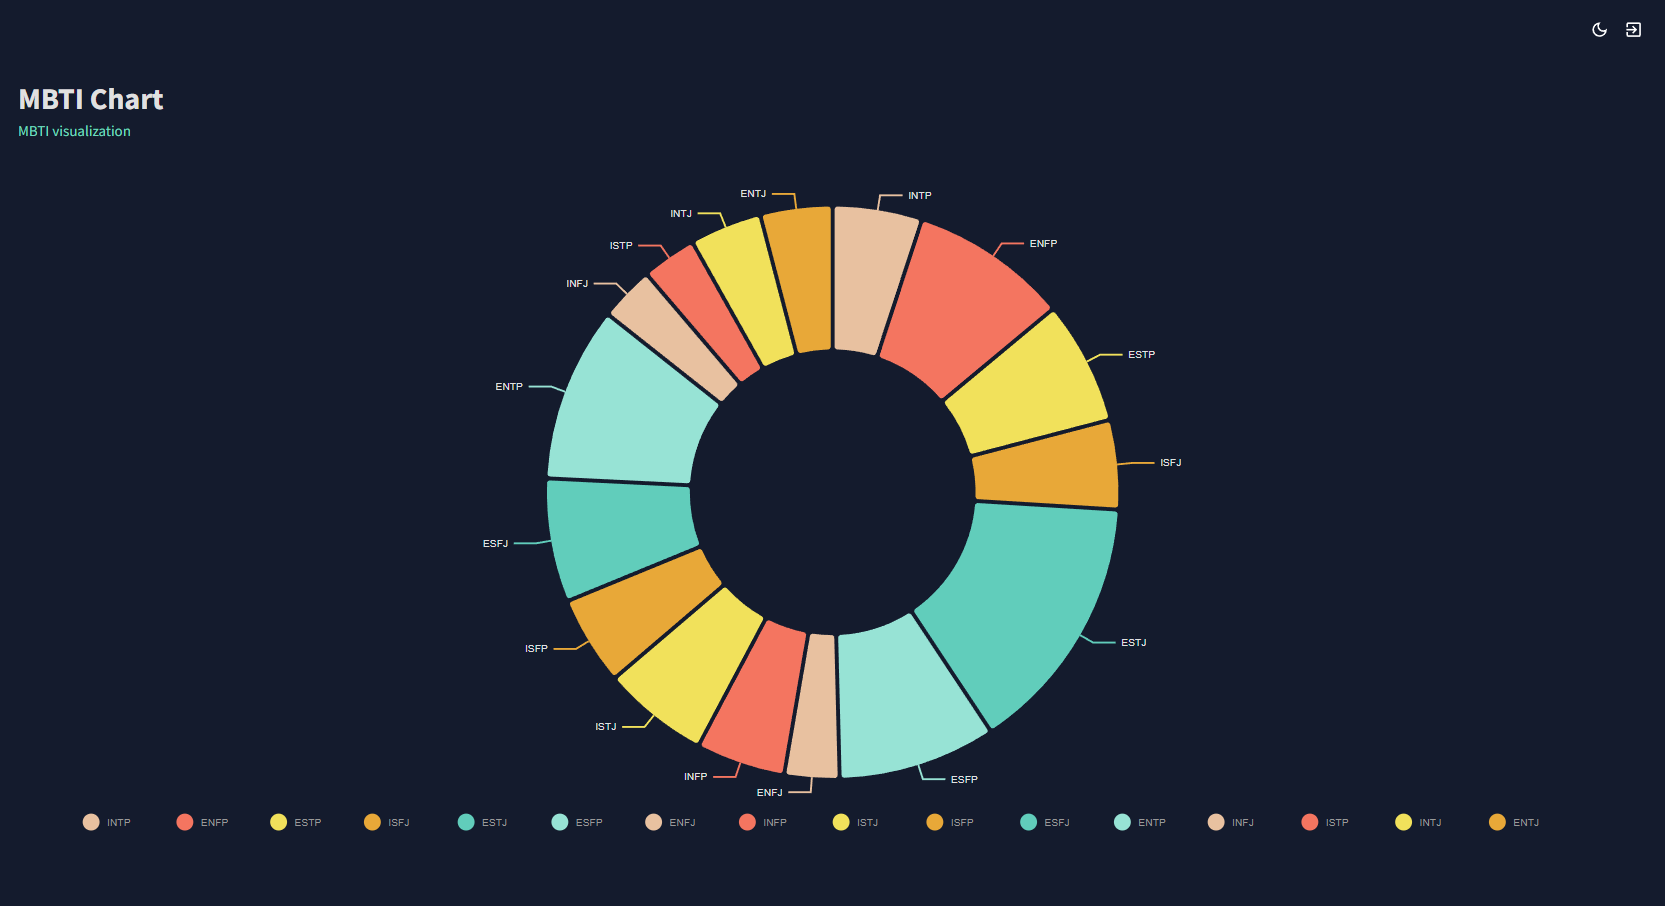
\includegraphics[width=0.75\linewidth]{mbtiChart.png}
    \vspace{0.6cm}
    \caption{Biểu đồ phân bố các nhóm tính cách MBTI dựa trên kết quả kiểm tra của người dùng}
\end{figure}

\subsubsection{Biểu đồ Career Clustering}
\begin{figure}[H]
    \centering
    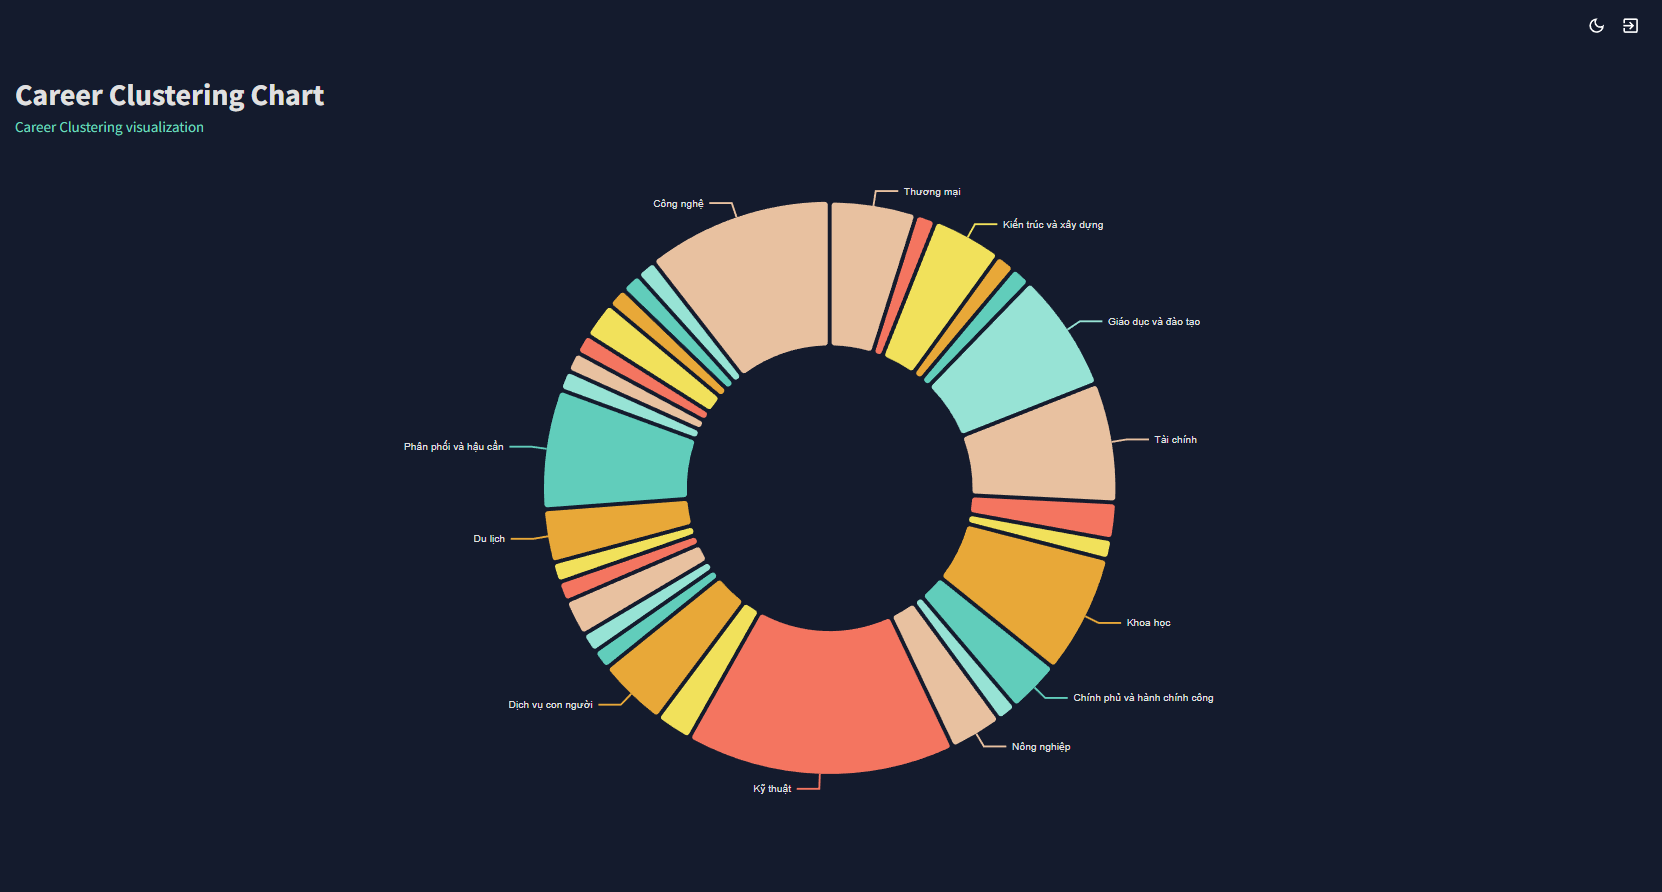
\includegraphics[width=0.75\linewidth]{images/CCChart.png}
    \vspace{0.6cm}
    \caption{Biểu đồ phân bố các nhóm nghề nghiệp dựa trên kết quả kiểm tra của người dùng}
\end{figure}

\subsection{Phân tích và trực quan hóa dữ liệu}
\label{sec:data_analysis}
\begin{figure}[H]
    \centering
    \includegraphics[width=0.75\linewidth]{images/admin.jpg}
    \vspace{0.6cm}
    \caption{Giao diện truy vấn trực tiếp dữ liệu}
\end{figure}

Trang này tập trung vào việc truy vấn và quản lý, bao gồm:
\begin{itemize}
    \item Thêm dữ liệu   mới vào để phân tích hoặc lựa chọn dữ liệu có sẵn
    \item Truy vấn dữ liệu trong khung query bằng ngôn ngữ tự nhiên.
\end{itemize}

Ngoài ra còn cung cấp bộ công cụ để người dùng tự trực quan hóa dữ liệu của mình.
\begin{figure}[H]
    \centering
    \includegraphics[width=0.75\linewidth]{images/admin2.jpg}
    \vspace{0.6cm}
    \caption{Giao diện trực quan hóa dữ liệu}
\end{figure}

\begin{itemize}
    \item Bộ công cụ để xây dựng truy vấn dữ liệu trực quan.
\end{itemize}
